%%%%%%%%%%%%%%%%%%%%%%%%%%%%%%%%%%%%%%%%%
% Masters/Doctoral Thesis 
% LaTeX Template
% Version 2.4 (22/11/16)
%
% This template has been downloaded from:
% http://www.LaTeXTemplates.com
%
% Version 2.x major modifications by:
% Vel (vel@latextemplates.com)
%
% This template is based on a template by:
% Steve Gunn (http://users.ecs.soton.ac.uk/srg/softwaretools/document/templates/)
% Sunil Patel (http://www.sunilpatel.co.uk/thesis-template/)
%
% Template license:
% CC BY-NC-SA 3.0 (http://creativecommons.org/licenses/by-nc-sa/3.0/)
%
%%%%%%%%%%%%%%%%%%%%%%%%%%%%%%%%%%%%%%%%%

%----------------------------------------------------------------------------------------
%	PACKAGES AND OTHER DOCUMENT CONFIGURATIONS
%----------------------------------------------------------------------------------------

\documentclass[
12pt, % The default document font size, options: 10pt, 11pt, 12pt
%oneside, % Two side (alternating margins) for binding by default, uncomment to switch to one side
spanish, % ngerman for German
singlespacing, % Single line spacing, alternatives: onehalfspacing or doublespacing
%draft, % Uncomment to enable draft mode (no pictures, no links, overfull hboxes indicated)
%nolistspacing, % If the document is onehalfspacing or doublespacing, uncomment this to set spacing in lists to single
%liststotoc, % Uncomment to add the list of figures/tables/etc to the table of contents
%toctotoc, % Uncomment to add the main table of contents to the table of contents
%parskip, % Uncomment to add space between paragraphs
%nohyperref, % Uncomment to not load the hyperref package
headsepline, % Uncomment to get a line under the header
%chapterinoneline, % Uncomment to place the chapter title next to the number on one line
%consistentlayout, % Uncomment to change the layout of the declaration, abstract and acknowledgements pages to match the default layout
]{MastersDoctoralThesis} % The class file specifying the document structure

\usepackage[utf8]{inputenc} % Required for inputting international characters
\usepackage[T1]{fontenc} % Output font encoding for international characters
\usepackage{graphics}
\usepackage{utopia} % Use the Palatino font by default
\usepackage[spanish]{babel}
\usepackage[latin1]{inputenc}
%\usepackage{arial}
\usepackage[backend=bibtex,style=authoryear,natbib=true]{biblatex} % Use the bibtex backend with the authoryear citation style (which resembles APA)
%\usepackage[natbibapa]{apacite}
%\bibliographystyle{apacite}

\addbibresource{Bib_Adrifelcha.bib} % The filename of the bibliography

%\usepackage[autostyle=true]{csquotes} % Required to generate language-dependent quotes in the bibliography

%----------------------------------------------------------------------------------------
%	MARGIN SETTINGS
%----------------------------------------------------------------------------------------

\geometry{
	paper=a4paper, % Change to letterpaper for US letter
	inner=2.5cm, % Inner margin
	outer=3.8cm, % Outer margin
	bindingoffset=.5cm, % Binding offset
	top=1.5cm, % Top margin
	bottom=1.5cm, % Bottom margin
	%showframe, % Uncomment to show how the type block is set on the page
}

%----------------------------------------------------------------------------------------
%	THESIS INFORMATION
%----------------------------------------------------------------------------------------

\thesistitle{Estudios con Detección de Señales} % Your thesis title, this is used in the title and abstract, print it elsewhere with \ttitle
\supervisor{Dr. Arturo Bouzas Riaño}%\textsc{Bouzas}} % Your supervisor's name, this is used in the title page, print it elsewhere with \supname
\examiner{Dr. Germán Palafox Palafox}%\textsc{Palafox}} % Your examiner's name, this is not currently used anywhere in the template, print it elsewhere with \examname
\degree{Licenciatura en Psicología} % Your degree name, this is used in the title page and abstract, print it elsewhere with \degreename
\author{Adriana Felisa Chávez De la Peña}%\textsc{Chávez De la Peña}} % Your name, this is used in the title page and abstract, print it elsewhere with \authorname
\addresses{} % Your address, this is not currently used anywhere in the template, print it elsewhere with \addressname

\subject{Psicología} % Your subject area, this is not currently used anywhere in the template, print it elsewhere with \subjectname
\keywords{Teoría de Detección de Señales, Memoria de Reconocimiento, Efecto Espejo, Ilusiones Ópticas, Modelamiento Bayesiano} % Keywords for your thesis, this is not currently used anywhere in the template, print it elsewhere with \keywordnames
\university{\href{http://www.university.com}{Universidad Nacional Autónoma de México}} % Your university's name and URL, this is used in the title page and abstract, print it elsewhere with \univname
\department{\href{http://department.university.com}{Laboratorio 25 de Comportamiento Adaptable}} % Your department's name and URL, this is used in the title page and abstract, print it elsewhere with \deptname
\group{\href{http://researchgroup.university.com}{Laboratorio de Comportamiento Adaptable}} % Your research group's name and URL, this is used in the title page, print it elsewhere with \groupname
\faculty{\href{http://faculty.university.com}{Facultad de Psicología}} % Your faculty's name and URL, this is used in the title page and abstract, print it elsewhere with \facname

\sinodalA{Dr. Óscar Zamora Arévalo}
\sinodalB{Mtro. Miguel Herrera Ortíz}
\sinodalC{Lic. José Luis Baroja Manzano}

\city{Ciudad de México}
\degreemonth{Noviembre}
\degreeyear{2017}

\proyectopapime{PAPIME PE310016}
\proyectopapiit{PAPIIT IN307214}

\AtBeginDocument{
\hypersetup{pdftitle=\ttitle} % Set the PDF's title to your title
\hypersetup{pdfauthor=\authorname} % Set the PDF's author to your name
\hypersetup{pdfkeywords=\keywordnames} % Set the PDF's keywords to your keywords
}

\begin{document}

\frontmatter % Use roman page numbering style (i, ii, iii, iv...) for the pre-content pages

\pagestyle{plain} % Default to the plain heading style until the thesis style is called for the body content

%----------------------------------------------------------------------------------------
%	TITLE PAGE
%----------------------------------------------------------------------------------------

\begin{titlepage}

\begin{minipage}[c][9in][s]{1in}
\centering
\hspace*{-0.2in} 
\includegraphics[width=1.1in]{Escudo-UNAM}\\[10pt]
\hskip 2pt\vrule width 2pt height 6.7in
\hskip 1mm\vrule width 1pt height 6.7in\\[10pt]
\hspace*{-0.2in} 
\includegraphics[width=1.2in]{PSI}
\end{minipage}\hskip 10pt
% Right layout - Titles
\begin{minipage}[c][\textheight][s]{5.125in}
\centering
% University, institute, department and title
{\Large\scshape\univname}
\vspace{3mm}\hrule height2pt
\vspace{1mm}\hrule height1pt
\vspace{3mm}
%\@ifundefined{\facname}{\relax}{{\large\scshape\facname}\\[3pt]}
{\scshape\facname}\par
% Title
\vfill\vfill
{\def\baselinestretch{1}\LARGE\scshape\ttitle\par}
\vfill\vfill
% Degree, author, supervisor and date
\makebox[8cm][s]{\Huge T E S I S}\\[8pt]
QUE PARA OBTENER EL GRADO DE:\\[8pt]
{\scshape\degreename}\\[16pt]
{\huge P  R  E  S  E  N  T  A:}\\[8pt]
{\large {\scshape\authorname}}\par
\vfill
{\small DIRECTOR DE TESIS:\\{\scshape\supname}}\par
\vfill
{\small REVISOR:\\{\scshape\examname}}\par
\vfill
{\small SINODALES:\\{\scshape\SinodalA}}\\{\scshape\SinodalB}}\\{\scshape\SinodalC}}\par
\vfill
{\small Con el apoyo de:\\Proyecto {\scshape\PAPIIT} y \\Proyecto {\scshape\PAPIME}}\par
\vfill
%{\today}
{\hspace*{0.2in}\scshape\city\hfill\today}
\end{minipage}
\end{titlepage}
\begin{titlepage}
\centering\large
{\def\baselinestretch{1.2}\Large\bfseries\ttitle\par}\\
\vspace{15mm}
por\par
\vspace{15mm}
{\Large\authorname}
\vspace{40mm}
\par
Tesis presentada para obtener la\par
\vspace{15mm}
\degreename\par
\vspace{15mm}
en la\par 
\vspace{15mm}
\facname
\par
\vspace{15mm}
{\Large\scshape\univname}
\vspace{30mm}
\par
\city, \today
\end{titlepage}}



%----------------------------------------------------------------------------------------
%	DECLARATION PAGE
%----------------------------------------------------------------------------------------

\begin{declaration}
\addchaptertocentry{\authorshipname} % Add the declaration to the table of contents
\noindent Yo, \authorname, declaro que la tesis aquí presentada bajo el título \enquote{\ttitle}, es de mi entera autoría, aclarando que:\\

\begin{itemize} 
\item La presente tesis fue desarrollada en el Laboratorio 25 de la Facultad de Psicología de la Universidad Nacional Autónoma de México, bajo la tutela del Dr. Arturo Bouzas Riaño. 
\item Ningún dato aquí presentado ha sido utilizado con anterioridad para recibir un grado académico ni en ésta ni en ninguna otra Universidad. 
\item Las ideas cuya autoría no me corresponde que son retomadas en el texto, están clara y adecuadamente señaladas. 
\item Así mismo, he señalado y dado crédito a toda fuente y material de apoyo consultados (lenguajes de programación, códigos base y manuales).
\item Todas las figuras que se presentan a lo largo de la presente tesis fueron elaboradas por la autora de la misma, por medio de los IDE's RStudio (para R) y Spyder (para Python), excepto cuando se señala lo contrario.
%\item Cualquier porción del trabajo aquí expuesto que se haya realizado en colaboración directa o indirecta con un tercero, es señalada y presentada con claridad.
\item El presente proyecto de investigación fue realizado con el apoyo de PAPIIT IN307214 y PAPIME PE310016.\\
\end{itemize}
 
\noindent Firma:\\
\rule[0.5em]{25em}{0.5pt} % This prints a line for the signature
 
\noindent Fecha:\\
\rule[0.5em]{25em}{0.5pt} % This prints a line to write the date
\end{declaration}

\cleardoublepage

%----------------------------------------------------------------------------------------
%	QUOTATION PAGE
%----------------------------------------------------------------------------------------

\vspace*{0.2\textheight}

\noindent\enquote{\itshape Research is what I'm doing when I don't know what I'm doing.}\bigbreak

%My experiences with science led me to God. They challenge science to prove the existence of God. But must we really light a candle to see the sun?
%1972

%Read more at: https://www.brainyquote.com/quotes/authors/s/steven_pinker_2.html
\hfill Wernher von Braun, 1957.\\

\vspace*{0.3\textheight}

\hfill(Apparently, I've been doing research my whole life\ldots)

%----------------------------------------------------------------------------------------
%	ABSTRACT PAGE
%----------------------------------------------------------------------------------------

\begin{abstract}
\addchaptertocentry{\abstractname} % Add the abstract to the table of contents

En estudios de Memoria de Reconocimiento donde se ha aplicado la Teoría de Detección de Señales para comparar el desempeño de los participantes entre clases de estímulos que se distinguen por la presición con que sus elementos se reconocen al ser presentados más de una vez -habiendo una clase que se reconoce con mayor facilidad (\textit{A}) que en la otra (\textit{B})-, se ha encontrado evidencia consistente de que dicha discrepancia se refleja simultáneamente en el número de Hits y Falsas Alarmas cometidas en cada una -$F.Alarmas(A) < F.Alarmas (B) < Hits(B) < Hits(A)$ - un patrón que sería identificado en la literatura como Efecto Espejo. Sin embargo, la extensión de este patrón a otras áreas no ha sido explorada todavía y su estudio e interpretación se ha restringido al dominio específico de las tareas de reconocimiento. En el presente trabajo se muestra evidencia del Efecto Espejo en una tarea de detección perceptual que incluye protocolos de respuesta binaria y de escala de confianza, donde los niveles de discriminabilidad a comparar fueron construidos con base en lo que se sabe sobre la Ilusión de Ebbinghaus. Los resultados obtenidos fueron evaluados tanto a partir de la replicación del análisis clásico (pruebas t y ANOVAS), como con la construcción de Modelos Bayesianos.

\end{abstract}

%\ldots
%----------------------------------------------------------------------------------------
%	ACKNOWLEDGEMENTS
%----------------------------------------------------------------------------------------

\begin{acknowledgements}
\addchaptertocentry{\acknowledgementname} % Add the acknowledgements to the table of contents

1. A mi familia\\

%Las primeras personas en quienes pienso al leer la palabra \textit{Agradecimiento} son mis padres, Sandra Amada De la Peña Cortina y David Chávez Granados. ¡A ustedes les debo cuanto soy y tengo! Mamá, gracias por enseñarme a no conformarme nunca y a dar siempre un poquito más, porque sé que -aunque no siempre te lo diga- es gracias a ti que soy quien soy. Papá, gracias por siempre confiar en mí y por el eterno apoyo que me has dado, ¡gracias por ser mi Superman!. Y sobretodo, quiero agradecer a los dos por la paciencia que me tuvieron durante este larguísimo proceso de titulación.\\

%Gracias a mi hermana Angélica -¡'la Enana'!- por ser la mejor compañera de aventuras, cómplice y confidente que pude haber deseado desde su llegada al mundo. La vida sería una carga mucho más pesada sino tuviera a la enana -pegada a su computadora- esperando en nuestro cuarto, dispuesta a escuchar las patoaventuras y dilemas existenciales de su hermana mayor.\\

%Gracias Juan Pablo Aguayo Chávez -¡JUANCHO!- por ser mi hermano mayor. Me llena de un profundo orgullo verte crecer en lo personal y profesionalmente. Tu hambre de éxito y aventura te llevará lejos, ¡y me hará muy feliz ser testigo de ello!\\

%Gracias a la familia Mejía-Chávez por todo su apoyo e interés. ¡Nunca olvidaré el gran cariño con que me recibieron aquella primera noche en el Shaky's Pizza! En el sentido estricto de las cosas yo era sólo una desconocida que ustedes nunca habían visto antes, y sin embargo, siempre me sentí parte de ustedes.\\

%Gracias a la familia Jiménez-Lloyd por recibirme en su hogar como si fuera una más de su familia. Richard y Claudia Jiménez son los nombres de un par de huellas que llevo en mi corazón, que me recuerdan que en el mundo habemos más personas buenas que egoístas, a quienes siempre recordaré con mucho amor y ternura.\\

%Gracias a la familia que me ha acompañado siempre. Gracias a mis abuelitos Lupe y Juan que siempre han estado al pendiente de a su nieta más distante; a mis padrinos, Grisel y Tomás, por cada muestra de amor y apoyo que me han obsequiado; a mis 'hermanos', JuanMa y Moni, que pese a la distancia y la brecha generacional me han hecho sentir su apoyo y cariño incondicional; a mi primo-hermano (literalmente) Juancho, con quien crecí y quien año con año cuando me hace admirarlo más cuando lo veo realizar sus sueños y proyectos; y a Peter por ser siempre un ejemplo a seguir, el hermano mayor que siempre quise tener.\\ 

2. A Jaime\\

%Muchísimas gracias a Jaime Osvaldo Islas Farias -mi amor, mi vida, ¡mi compañero de equipo!- por todo, absolutamente todo lo que hemos compartido. Las palabras que vienen a mi mente para expresar cuán en deuda estoy con la vida por permitirnos encontrarnos no hacen justicia a la emoción que siento, aún después de cuatro años juntos, cada vez que te veo. Jaime, conquistar tu corazón ha sido mi mayor logro.\\

3. Al Lab25\\

%Primero, gracias a los 'big guns' del Lab25: Manuel Villareal, José Luis Baroja y Melisa Chávez. Realmente no creo que tengan una idea de cuánto los he admirado desde mi llegada al lab y 

%Gracias a Elena Villalobos, por ser un recordatorio constante de la importancia que la constancia y la pasión por lo que se hace.\\

%En general, gracias a todos los miembros del Lab25 por su retroalimentación en seminarios y presentaciones: Victoria Torres, Alfonso Medina, Yuznhio Sierra, Paulina Eckerle, Karina Ruíz, Álvaro Zacarías, Ángel Garduño, Itzel Laurel, Carlos Velázquez, Mauricio Hernández, Stéphane Lejars y Diana Álvarez.\\

%Pero con especial énfasis y cariño, quiero agradecer a mis amigos José Manuel Niño y Uriel O. González Bravo. Amiguitos, sabemos que sin ustedes habría terminado la tesis mucho más rápido... pero también, que sin ustedes mi vida habría seguido cayendo en picada. Sé que ustedes saben que contar contar con su compañía, su atención y apoyo, y sobretodo su ácido sentido del humor realmente marcó un 'Antes' y un 'Después' para mí. De corazón, gracias por regresarme las ganas de levantarme por la mañana. Porque entre broma y broma, la verdad es que nadie sabe lo que este proceso ha sido para mí como ustedes dos. ¡Los quiero muchísimo, amiguitos!\\

%Niño, muchísimas gracias por el tiempo que me obsequiaste siendo el primer revisor "no-oficial" de este trabajo. Dices que no reconoces el título 'amigo', y sin embargo, quiero que sepas que sin considerarme tu amiga, haz hecho por mí mucho más que la mayoría de la gente a la que yo sí he asignado esa etiqueta. No tengo forma de agradecer el oído que siempre me has brindado. Eres alguien a quien tengo en alta estima; si la vida fuera un libro, tu serías mi personaje favorito.\\

%Uri, te quiero muchísimo. Sabes que siempre vas a contar con mi apoyo incodicional y que, siempre que necesites algo, podrás encontrarme.\\

4. A mis amigos\\

%Gracias a Alberto Carrera Mondragón -¡Lito!- por mantenerme cuerda, sana y salva durante mi paso por la carrera. \\

%A Alejandro Vázquez Calderón -¡Conejo!- por todo lo que haz hecho por mí, y por todas las tardes de café en que aguantaste mi parlanchinería y me permitiste desahogar mis conflictos existenciales. Gracias por demostrarme que cuando se quiere a alguien, se hace todo por estar ahí, no importa cómo.\\

%A Sol Fernández Rodríguez -Solesiwi-, por regresarle el sentido a la expresión \textit{'mejor amiga'}. Gracias por toda tu paciencia y empatía; gracias por esa don casi mágico que tienes para aterrizar mis pies en la tierra y traducir mis tormentos en soluciones concretas; gracias por siempr tener tiempo para escucharme, y sobretodo, gracias por ser el excelente ser humano que eres, e iluminar a quienes te rodeamos con tu ejemplo.\\

%Gracias a todos quienes de una u otra forma me acompañaron a lo largo de la carrera y a quienes les tocó verme vagar sin sentido durante la realización de la presente tesis. Gracias a Javier Alfaro Vega -Javs- por siempre, siempre, hacerse un tiempo para verme cuando más necesité a alguien que me escuchara; a Andrea Chávez -Andy- por ser el epítome de la honestidad y la bondad; a Brandon Carmona por ser mi amigo en esta y todas las vidas que he vivido; a Avinash Mercado por siempre tener algo nuevo, interesante (y random) que enseñarme; a Maximiliano Hinojosa -Max- por ser el ser más enigmático de la galaxia y aún así, ser amigo de una persona tan ordinaria como yo; a Martin Hernández por toda su paciencia a lo largo de estos años; y a Edgar Vázquez, un ser humano realmente increíbl, cuyos constantes logros me motivan a esforzarme siempre un poquitito más.\\

5. A los honorables académicos e investigadores que me apoyaron como sinodales.\\

%Gracias al Doctor Germán Palafox Palafox por permitirme contar con su apoyo como Revisor del presente proyecto de tesis.\\

%Gracias al Dr. Óscar Zamora Arévalo por fungir como mi primer sinodal y acompañarme en este proceso de titulación con que concluyo mi formación académica en la Licenciatura. 

%Gracias al Mtro. Miguel Herrera Ortiz por todo el apoyo que me ha brindado desde que fuere su alumna en la licenciatura. La perspectiva tan amplia y la narrativa tan mágica con que usted suele presentar -y dar sentido, como si fuera parte de un mismo conjunto- el estudio de la Cognición y la Toma de Decisiones, fue la principal razón por la que decidí orientar el resto de mi formación hacia la Psicología Experimental.

%Gracias al Lic. José Luis Baroja Manzano por acceder a ser uno de mis sinodales en este tortuoso camino llamado 'titulación'. José Luis, no sé si ya te lo he dicho, pero eres alguien a quien admiro profundamente. Desde que entré al Lab25 por allá del 2015, has sido una figura muy importante para mí,

6. Last but not least... al Doc.\\

%Y sobre todo, "last but not least", agradezco infinitamente al Dr. Arturo Bouzas por brindarme la oportunidad de trabajar bajo su guía, por permitirme el honor de llamarme su estudiante y por todas las oportunidades de crecimiento que puso a mi alcance. Sé que el tema que decidí trabajar no es precisamente 'su mero mole' y sin embargo, siempre me dio libertad de trabajar en lo que a mí me gustaba. Por éso y por la confianza que depositó en mí al permitirme colaborar en los diversos proyectos del laboratorio, es que siempre será para mí EL 'Doc'.\\

%\ldots
\end{acknowledgements}

%----------------------------------------------------------------------------------------
%	LIST OF CONTENTS/FIGURES/TABLES PAGES
%----------------------------------------------------------------------------------------

\tableofcontents % Prints the main table of contents

\listoffigures % Prints the list of figures

\listoftables % Prints the list of tables

%----------------------------------------------------------------------------------------
%	ABBREVIATIONS
%----------------------------------------------------------------------------------------

\begin{abbreviations}{ll} % Include a list of abbreviations (a table of two columns)

\textbf{AUC} & \textbf{A}rea-\textbf{U}nder (the) \textbf{C}urve\\
\textbf{CDF} & \textbf{C}umulative \textbf{D}ensity \textbf{F}unction\\
\textbf{CSV} & \textbf{C}omma \textbf{S}eparated \textbf{V}alues\\
\textbf{JASP} & \textbf{J}effrey's \textbf{A}mazing \textbf{S}tatistics \textbf{P}rogran\\
\textbf{SDT} & \textbf{S}ignal \textbf{D}etection \textbf{T}heory\\
\textbf{ROC} & \textbf{R}eceiver-\textbf{O}perating \textbf{C}haracteristic curve\\
\textbf{RT} & \textbf{R}esponse \textbf{T}ime\\
\textbf{MOC} & \textbf{M}emory-\textbf{O}perating \textbf{C}haracteristic curve\\

\end{abbreviations}


%----------------------------------------------------------------------------------------
%	DEDICATION
%----------------------------------------------------------------------------------------

\dedicatory{En Memoria de\\\\
María Eugenia Leticia De la Peña Cortina\\
(1956-2011)\\\\
 y\\\\
 Tomás Munguía Ramírez\\
 (1958-2017)} 


%\vspace*{0.2\textheight}

%\noindent\enquote{\itshape Arriésgate, equivócate, cáete... pero vive.}\bigbreak

%\hfill Mi tía Letty, \\Mayo del 2009.


%----------------------------------------------------------------------------------------
%	THESIS CONTENT - CHAPTERS
%----------------------------------------------------------------------------------------

\mainmatter % Begin numeric (1,2,3...) page numbering

\pagestyle{thesis} % Return the page headers back to the "thesis" style

% Include the chapters of the thesis as separate files from the Chapters folder
% Uncomment the lines as you write the chapters

% Chapter 1

\chapter{Introducción} % Main chapter title

\label{Chapter1} % For referencing the chapter elsewhere, use \ref{Chapter1} 

%----------------------------------------------------------------------------------------

% Define some commands to keep the formatting separated from the content 
\newcommand{\keyword}[1]{\textbf{#1}}
\newcommand{\tabhead}[1]{\textbf{#1}}
\newcommand{\code}[1]{\texttt{#1}}
\newcommand{\file}[1]{\texttt{\bfseries#1}}
\newcommand{\option}[1]{\texttt{\itshape#1}}

%----------------------------------------------------------------------------------------

El mundo está cargado de ruido e incertidumbre. Los organismos están constantemente expuestos a distintas fuentes de estimulación en su entorno que pueden proporcionar, o no, información relevante sobre el estado de las cosas y las reglas vigentes. Por ello, uno de los primeros grandes problemas de adaptabilidad a los que se enfrentan los organismos consiste en ordenar el caos resultante, definiendo relaciones de contingencia que les permitan hacer predicciones sobre la disponibilidad de ciertos sucesos biológicamente importantes y ajustar su comportamiento a las restricciones operantes. Una vez establecida la relación entre la presencia u ocurrencia de ciertos estímulos y el acceso a ciertas consecuencias, la detección de éstos se vuelve una tarea importante para que los organismos puedan guiar su comportamiento, (por ejemplo: \textit{'Sé que soy alérgico a las nueces, ¿En este panqué hay nueces? Si hay nueces en el panqué, no lo como; si no hay nueces en el panqué, sí lo como.'}).\\


%La detección de ciertos eventos no es una tarea sencilla. La información a evaluar suele ser ambigua.
Detectar algo no parecería ser un problema importante si asumiéramos que todo evento aparece con perfecta claridad, o bien, que el organismo interesado en su detección cuenta con sensores altamente precisos que le garantizan el éxito. Sin embargo, la evidencia a partir de la cual juzgamos si algo está ocurriendo o no, por lo general es confusa y puede llevarnos a emitir juicios erróneos. Como un ejemplo cotidiano, imaginemos el caso de un adolescente que quiere conseguir permiso para ir a una fiesta y necesita encontrar el momento ideal para pedírselo a su mamá (\textit{cuando ella esté de buen humor}). Los indicadores con que cuenta son imprecisos (los gestos, el tono de voz, las actividades que su madre realice durante el día, etc.), por lo que puede errar en el diagnóstico del estado emocional de su madre y no obtener el permiso deseado, ya sea por una mala lectura de los datos disponibles (que las ansias del adolescente por salir de fiesta le hagan apresurar el momento) o bien porque los datos en sí mismos son poco claros (la mamá podría ser una persona particularmente inexpresiva o, por el contrario, altamente variable).\\ 

%La detección es distinta de la discriminación y la categorización. Todos problemas importantes en un entorno cargado de estimulación. (El problema del embudo)
%A diferencia de problemas tales como la discriminación o la categorización, donde la tarea de los organismos es evaluar la evidencia que se les presenta para asignarle una etiqueta (tales como \textit{'¿Es A o es B?'} ó \textit{'De acuerdo a sus propiedades en tales dimensiones, se trata de un caso de...'}), cuando hablamos de un problema de detección nos referimos a situaciones que pueden plantearse en términos de \textit{preguntas Sí/No}, (por ejemplo, \textit{'¿La comida está buena? Sí/No'}, \textit{'¿Ese que viene es mi camión? Sí/No'}, \textit{'¿Este perro es hostil? Sí/No'}) y cuya respuesta permite guiar el comportamiento de los organismos en función de las consecuencias anunciadas (\textit{'Sí, la comida está buena, me la comeré porque es seguro'}, \textit{'No, ese no es mi camión, no me subiré porque acabaré en Ecatepec'}, \textit{'No, no es un perro hostil, puedo acariciarlo'}, etc.).\\ 

La Teoría de Detección de Señales (SDT en ingles) presenta un modelo estadístico que describe las tareas de detección como un problema de decisión al que tienen que enfrentarse los organismos, sistemas inmersos en entornos con incertidumbre -es decir, entornos dinámicos que presentan variabilidad en la disponibilidad y presentación de ciertos eventos-, para guiar su comportamiento de la manera más óptima posible dada la estructura del mismo (Peterson, Birdsall y Fox, \citeyear{Peterson1954}; Tanner y Swets, \citeyear{Tanner1954}; Kileen, \citeyear{Killeen2014}). La SDT funciona tanto como un modelo estadístico para describir esta clase de problemas, como una herramienta para interpretar la ejecución de sistemas evaluados experimentalmente y hacer inferencias sobre la precisión con que los eventos a detectar (las señales) se distinguen del ruido que les rodea y la posible preferencia del sistema a responder en favor o en contra de su detección (Stainslaw y Todorov, \citeyear{Stainslaw1999}). Se trata de uno de los modelos más sólidos y ampliamente estudiados en Psicología Experimental, cuyos supuestos son lo suficientemente generales para permitir su aplicación al estudio de distintos fenómenos. \\

La SDT le concede a la noción de variabilidad un papel fundamental en su definición de la detección de señales como un problema de adaptabilidad. La idea básica es que las señales cuya detección resulta relevante para los organismos suelen presentarse y percibirse con cierta variabilidad y que, además de ello, coexisten en el mundo con otros estímulos (el ruido) que, dada su propia variabilidad, pueden llegar a ser confundidos con éstas (Tanner y Swets, \citeyear{Tanner1954}; Swets, \citeyear{Swets1973}). Por ejemplo, imaginemos que queremos detectar si la persona que nos acaba de contestar el teléfono es un adulto. Existe un rango de tonos de voz que asociamos con las personas adultas y que, a grandes rasgos, es más grave de lo que esperaríamos escuchar en un niño. Sin embargo, sabemos que hay adultos que pueden tener voces particularmente agudas y que pueden confundirse con la de un menor de edad: si quien nos contestó el teléfono tiene una voz aguda, no podremos estar seguros de si se trata de un adulto -o no- y tendremos que actuar conforme lo que nos parezca más probable.\\

La SDT opera como un modelo de decisión, en tanto que no asume que los organismos detectan los elementos relevantes en su entorno como respuesta directa a la estimulación que reciben momento a momento (como ocurre en las Teorías de Umbral que le preceden), sino que esta evidencia es ponderada por el sistema detector con la información que posee sobre el escenario en que se encuentra (Killeen, \citeyear{Killeen2014}). Bajo esta visión, los organismos \textit{eligen} el juicio de detección que les permite guiar su comportamiento de la manera más óptima posible tomando en cuenta: 1) las ganancias y pérdidas que están en juego -y que hacen más o menos importante el cometer cierto tipo de acierto o evitar cierto tipo de error- y 2) la probabilidad con que dichos eventos se presentan en su entorno. De esta forma, la noción de los umbrales ampliamente desarrollada en la Psicofísica clásica es reemplazada por los criterios de elección, (Wickens \citeyear{Wickens1}).\\ 

Al aplicar la SDT en tareas de memoria de reconocimiento -donde los participantes tienen que identificar los elementos ya antes vistos (las señales) dentro de un conjunto de ítems que contiene tanto elementos de una fase previa como elementos nuevos (el ruido)- para comparar la ejecución de los participantes entre dos clases de estímulos A y B, (siendo que A es más fácil de reconocer que B), se ha encontrado consistentemente un patrón de respuestas que demuestra que los participantes no sólamente son mejores reconociendo las señales de la condición A ($Hits(A)>Hits(B)$), sino que también son mejores identificando los estímulos con ruido de esta misma condición ($F.alarm(A)<F.alarm(B)$). En este tipo de estudios, los estímulos de las clases A y B son presentados de manera aleatoria, sin que se les informe a los participantes de la diferencia entre estos y por tanto, se asume que sus respuestas son emitidas en función a un único criterio de elección. De acuerdo con las tasas de Hits y Falsas Alarmas registradas por cada clase, parece ser que las distribuciones de Ruido y Señal de las clases A y B, se despliegan a lo largo de un mismo eje de evidencia \textit{reflejándose} entre sí -siendo que las distribuciones de la clase A aparecen a los extremos del eje, con muy poco sobrelape entre sí, y las distribuciones de la clase B, situadas en el centro, presentan la mayor incertidumbre- razón por la que dicho patrón de respuestas ha sido referido como Efecto Espejo (Glanzer y Bowles, \citeyear{Glanzer1976}; Glanzer, Adams, Iverson y Kim, \citeyear{Glanzer1993}).\\

%3.5*42.5
El Efecto Espejo sólo ha sido estudiado dentro del dominio de la memoria de reconocimiento, donde se ha reportado a lo largo de una amplia variedad de procedimientos y variables (Glanzer y Adams, \citeyear{Glanzer1990}). Como resultado, gran parte de los intentos por dar cuenta de este fenómeno se han desarrollado en torno a la estructura de las tareas de reconocimiento, por lo general, asumiendo que existen diferencias importantes en la forma en que cada clase de estímulo es atendida, procesada y/o evaluada durante la fase de estudio (Glanzer, Adams, Iverson y Kim, \citeyear{Glanzer1993}; Glanzer, Kim y Adams, \citeyear{Glanzer1998}; Glanzer, Hilford y Maloney, \citeyear{Glanzer2009}). Es decir, que bajo esta perspectiva el Efecto Espejo ha sido tratado como reflejo de los procesos cognitivos compreometidos en las tareas memoria de reconocimiento.\\

El interés principal del presente trabajo de tesis fue explorar la generalizabilidad del Efecto Espejo, buscando evidencia del mismo en una tarea de detección ajena a la memoria de reconocimiento. Para ello, se presentan dos variaciones de una tarea de detección perceptual (visual) que emula la estructura de los estudios donde ha sido reportado, construyendo dos niveles de dificultad con base en la literatura en ilusiones ópticas. La tarea elaborada fue presentada a los participantes a partir de dos protocolos: una tarea Sí/No y la asignación de puntajes en una Escala de Confianza. Los resultados e implicaciones de los mismos se discuten en detalle.\\
% Chapter 1
\chapter{Marco Teórico} % Main chapter title

\label{Cap_SDT} % For referencing the chapter elsewhere, use \ref{Chapter1} 

%----------------------------------------------------------------------------------------

% Define some commands to keep the formatting separated from the content 
\newcommand{\keyword}[1]{\textbf{#1}}
\newcommand{\tabhead}[1]{\textbf{#1}}
\newcommand{\code}[1]{\texttt{#1}}
\newcommand{\file}[1]{\texttt{\bfseries#1}}
\newcommand{\option}[1]{\texttt{\itshape#1}}

%----------------------------------------------------------------------------------------

\section{Teoría de Detección de Señales}

%Detectar ciertos estados en el mundo es importante para guiar nuestro comportamiento
Uno de los problemas más frecuentes a los que se enfrentan los organismos como sistemas inmersos en entornos variables que buscan optimizar su comportamiento, es la detección de estados o eventos específicos (\textbf{señales}) que de acuerdo a su experiencia y tras la definición de ciertas relaciones de contingencia, les proporcionen información relevante sobre el estado del mundo, las restricciones vigentes y la disponibilidad de eventos biológicamente importantes (McNicol, \citeyear{McNicol1}).\\

%Origen y expansión de la Teoría de Detección de Señales en la psicología y otras áreas
La Teoría de Detección de Señales (SDT, por sus siglas en inglés) aparece por primera vez en 1954 -como tantos otros avances científicos y tecnológicos motivados por las necesidades planteadas por la Segunda Guerra Mundial- en el contexto del estudio y desarrollo de radares para detectar señales eléctricas específicas (Peterson, Birdsall y Fox, \citeyear{Peterson1954}). Muy poco tiempo después, los psicólogos John A. Swets y Wilson P. Tanner contribuyeron a la expansión de la teoría a un contexto psicológico, como un modelo para estudiar la percepción de los organismos (Tanner y Swets, \citeyear{Tanner1954}; Swets, Tanner y Birdsall, \citeyear{Swets1961}). Desde entonces, la SDT constituye uno de los modelos más estudiados, desarrollados y ampliamente aplicados en Psicología (Stainslaw y Todorov, \citeyear{Stainslaw1999}), extendiéndose desde su foco inicial en el estudio de la percepción (Rosenholtz, \citeyear{Rosenholtz2001}; Pessoa, Japee y Ungerleider, \citeyear{Pessoa2005}; Wallis y Horswill, \citeyear{Wallis2007}) hacia el estudio de cualquier fenómeno o escenario donde los organismos se enfrenten al problema de emitir -y guiar su comportamiento en función a- juicios de detección; por ejemplo, en materia de la emisión de diagnósticos clínicos (Grossberg y Grant, \citeyear{Grossberg1978}; Swets, Dawes y Monahan, \citeyear{Swets2000}; Boutis, Pecaric, Seeto y Pusic, \citeyear{Boutis2010}), en el estudio de ciertas condiciones clínicas (Westermann y Lincoln, \citeyear{Westermann2010}; Bonnel y cols., \citeyear{Bonnel2003}; Brown, Kosslyn, Breiter, Baer y Jenike, \citeyear{Brown1994}; Naliboff y Cohen, \citeyear{Naliboff1981}), en el estudio de la identificación visual de testigos (Gronlund, Wixted y Mickes, \citeyear{Gronlund2014}; Wixted y Mickes, \citeyear{Wixted2014}; Wixted, Miches, Dunn, Clark y Wells, \citeyear{Wixted2016}) y un muy amplio \textit{etcétera} (Gordon y Clark, \citeyear{Gordon1974}; Nuechterlein, \citeyear{Nuechterlein1983}; Harvey Jr., Hammond, Lusk y Mross, \citeyear{Harvey1992}; Verghese, \citeyear{Verghese2001}).\\ 

%La Teoría de Detección de señales como un modelo descriptivo para el problema de la detección que admite la importancia de la incertidumbre, como parte del entorno y como motor en el uso de sesgos de respuesta.
La SDT constituye un modelo estadístico que describe el problema al que se enfrentan los organismos inmersos en situaciones de detección en ambientes con incertidumbre, donde las \textit{señales} -los estímulos cuya ocurrencia interesa detectar- coexisten con \textit{ruido} -estímulos que no son la señal pero que pueden confundirse con esta-. Se trata de un modelo de decisión que entiende la detección como una tarea de elección, donde los organismos no responden simplemente con base en lo que perciben, sino que emiten el juicio de detección que les permita guiar su comportamiento de la manera mas óptima posible dada la información que poseen sobre su entorno y la evidencia presente (Swets y cols., \citeyear{Swets2000}; Killeen, \citeyear{Killeen2014}).\\

La generalizabilidad del modelo de la SDT al estudio de distintos fenómenos y tareas de detección es posible gracias a lo abstracto de sus elementos: la señal que interesa detectar puede ser desde un estímulo concreto -una luz o un tono- hasta la pertenencia a una categoría -una enfermedad o amenaza- y el ruido es simplemente todo elemento presente en el entorno de la tarea que no sea la señal (Stainslaw y Todorov, \citeyear{Stainslaw1999}; McNicol, \citeyear{McNicol1}).\\ 

\subsection{Supuestos generales del modelo}

%La TDS distingue dos grandes factores en la emisión de un juicio o respuesta: La discriminabilidad y el sesgo.
La SDT funciona como una herramienta -o marco de análisis- para traducir el desempeño observado en tareas de detección en inferencias sobre la precisión con que la señal se distingue del ruido (la \textbf{discriminabilidad}) y la posible preferencia -o tendencia- del sistema detector a responder en favor o en contra de su detección, de acuerdo a la estructura de la tarea y las consecuencias comprometidas (el \textbf{sesgo}), (McNicol, \citeyear{McNicol1}). Esta distinción entre la discriminabilidad de los estímulos comprometidos y el sesgo del sistema, es una de las principales propiedades de la SDT (Swets y cols., \citeyear{Swets1961}) cuya importancia e implicaciones se discuten a continuación:\\

\textbf{1.- El papel de la Discriminabilidad: Siempre hay incertidumbre}\\

%Hay variabilidad en todos los estímulos implicados en las tareas de detección (en la señal y en los estímulos no-señal)
Se habla de la detección de señales como un problema de adaptabilidad porque se asume que la variabilidad en la presentación y percepción de los estímulos en el ambiente merma la capacidad de los organismos de emitir juicios de detección que reflejen el estado del mundo con certeza (Tanner y Swets, \citeyear{Tanner1954}). Y dado que los \textit{estímulos-Señal} coexisten en el mundo con \textit{estímulos-Ruido}, saber qué tan salientes son las señales respecto del ruido es uno de los factores más importantes para determinar qué tan difícil es su detección para los organismos. En términos de la SDT, se habla de dicha dificultad como \textit{la discriminabilidad} de los estímulos comprometidos en la tarea y suele explicarse en términos de:\\

%De acuerdo con la SDT, la discriminabilidad constituye el primer gran componente en la emisión de juicios de detección óptimos que reflejen el verdadero estado del mundo y permitan al organismo actuar conforme a las consecuencias vigentes. La discriminabilidad suele explicarse en términos de:\\ %  1) la variabilidad intrínseca en la presentación de las señales y 2) el ruido con que ésta coexiste.\\

\underline{a) La Variabilidad en la Señal}\\

%Existe variabilidad en la forma en que percibimos los estímulos que nos rodean. Los sistemas sensoriales y perceptuales se comportan como instrumentos de medición (error de medida)
La noción de variabilidad ha sido uno de los principales motores para el desarrollo de modelos estadísticos en Psicología. Desde que Fechner (\citeyear{Fechner}) extendió las ideas planteadas por Gauss (\citeyear{Gauss}) sobre la incertidumbre contenida en toda medición -la idea de que toda medición realizada contiene el valor \textit{verdadero} de aquello que se quiere medir más un \textit{error} aleatorio que la carga de incertidumbre- al estudio de la percepción, conceptualizando nuestros sistemas sensoriales y perceptuales como instrumentos de medición que en cada observación perciben las cualidades verdaderas de los estímulos más un error, se sentaron las bases para el desarrollo de una amplia gama de modelos matemáticos y estadísticos en Psicofísica orientados a estudiar la relación entre las cualidades físicas -\textit{reales}- de los estímulos y la magnitud o intensidad con que se perciben psicológicamente (Thurstone, \citeyear{Thurstone1927}; Swets, \citeyear{Swets1973}; Link, \citeyear{Link1994}).\\

%Variabilidad en la percepción de un mismo estímulo.
En el marco de la SDT, la variabilidad se considera una propiedad intrínseca de las señales a detectar bajo el supuesto de que ningún estímulo se percibe o se presenta de manera idéntica en cada exposición (Tanner y Swets, \citeyear{Tanner1954}). Por ejemplo, imaginemos los siguientes casos: \\

\begin{itemize}
\item Una persona es expuesta a un mismo tono con intensidad $X$ en cien ocasiones distintas y tras cada presentación, asigna un valor a la intensidad percibida. El valor reportado en cada ensayo será una mezcla entre el valor real del tono y un error aleatorio. Como se muestra en la Figura~\ref{fig:Senal_percepcion}, es muy probable que el valor percibido y reportado coincida con -o se acerque bastante a- su valor real (la media de la distribución, $\mu$, señalada con una línea vertical roja), pero también habrá ensayos en el valor percibido caiga por encima o por debajo de su valor real con cierta dispersión (las colas de la distribución). Existe variabilidad en la forma en que se perciben los estímulos.\\

\begin{figure}[h]
\centering
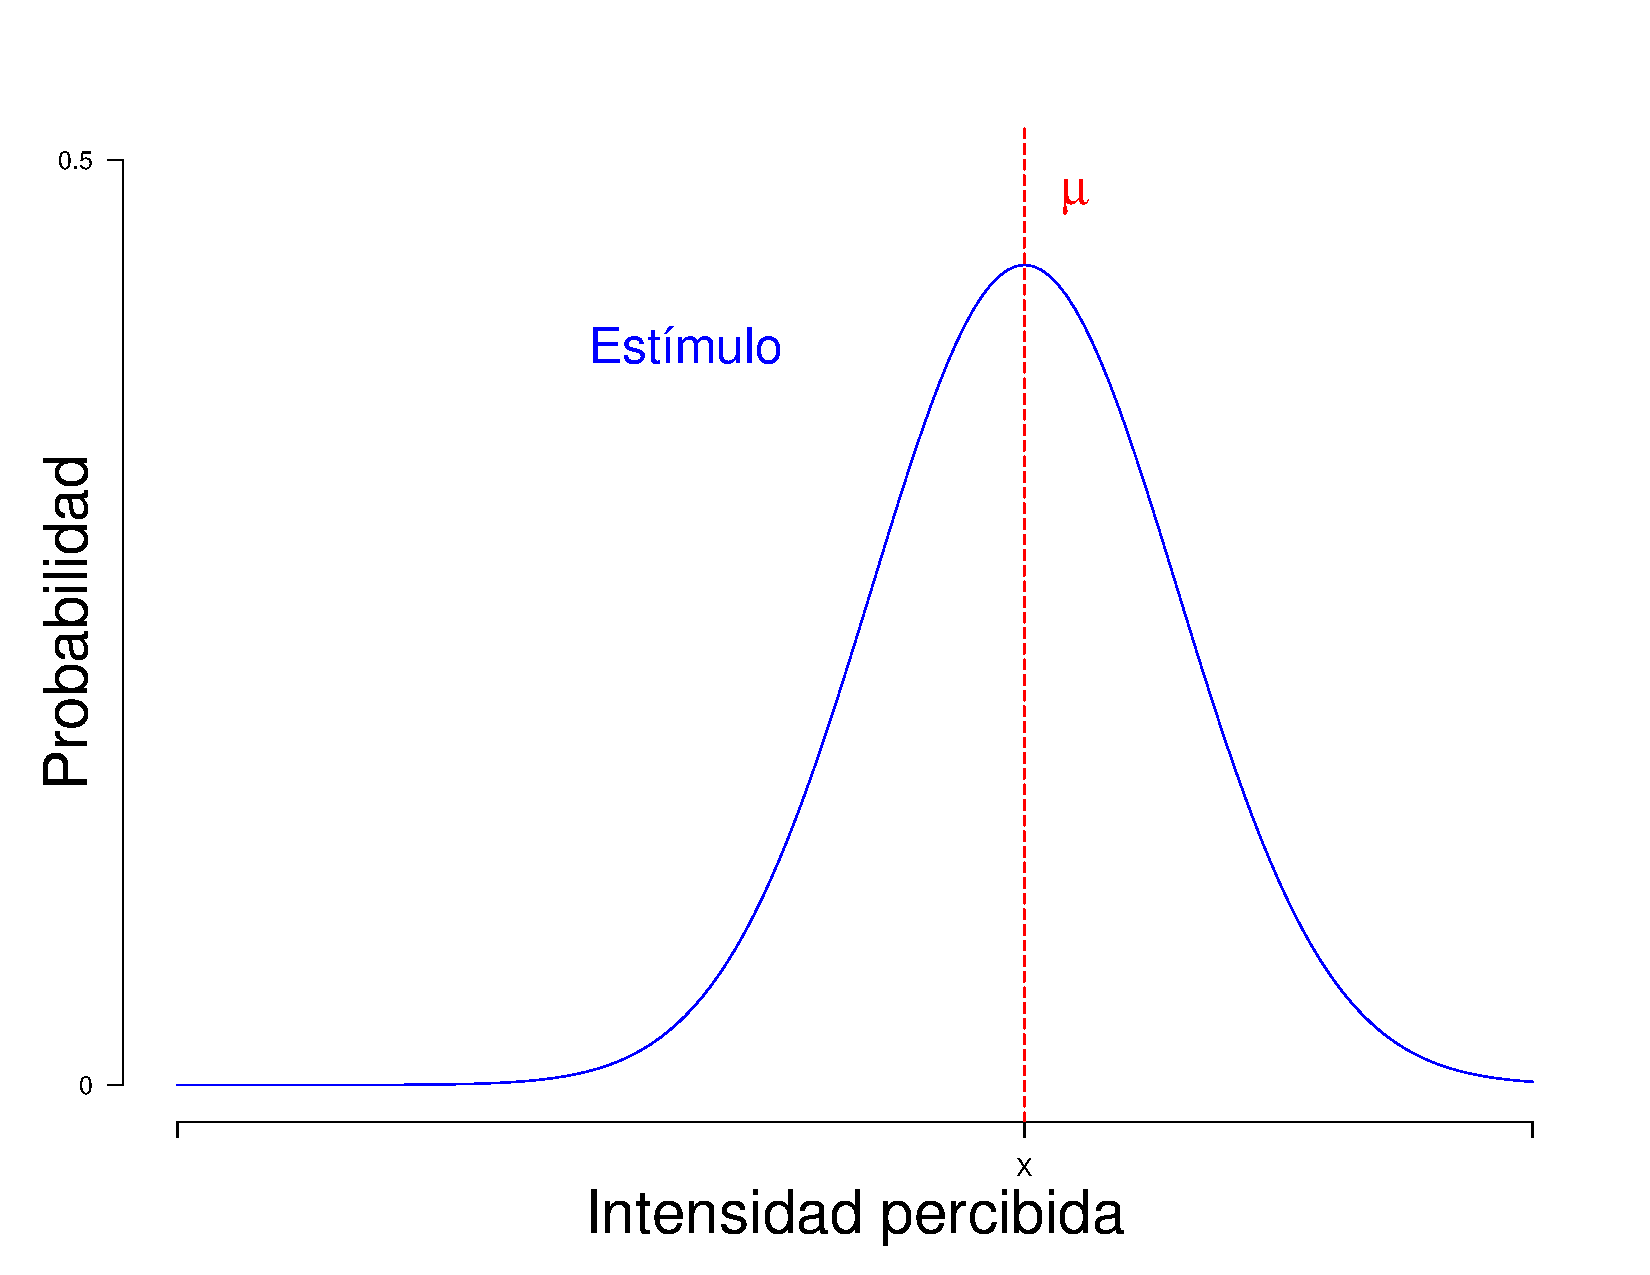
\includegraphics[width=0.75\textwidth]{Figures/Signal_Perception} 
%\decoRule
\caption[Variabilidad en la percepción de los estímulos]{La variabilidad en la percepción de los estímulos es ilustrada con una distribución de probabilidad normal: al presentar un estímulo con intensidad $x$ en repetidas ocasiones, es muy probable que el valor percibido se acerque a su valor real (la media, $\mu$), sin embargo, también puede percibirse con mayor o menor intensidad.}
\label{fig:Senal_percepcion}
\end{figure}

\item Un psicólogo aplica una prueba clínica \textit{A} para evaluar si su paciente tiene depresión. Por lo general, las pruebas clínicas arrojan un puntaje \textit{p} que, de acuerdo a su correspondencia con el rango de puntajes típicamente obtenidos por personas que tienen cierta condición, sugieren el diagnóstico a emitir. La Figura~\ref{fig:Senal_presentacion}, ~\ref{fig:Senal_presentacion2} presenta la idea central de este ejemplo: no todas las personas con depresión obtienen exactamente el mismo puntaje, sino que dentro de la serie de posibles puntajes a obtener en la prueba (todos los valores en el eje de las x), las personas con depresión suelen obtener resultados dentro de un rango específico con cierta probabilidad (la distribución azul), de tal suerte que hay puntajes que se asocian con dicha condición con mayor probabilidad (siendo la media de la distribución, $\mu$, señalada en rojo la más probable), que otros. También existe variabilidad en la presentación de ciertos estímulos en el entorno.\\
\end{itemize}

\begin{figure}[h]
\centering
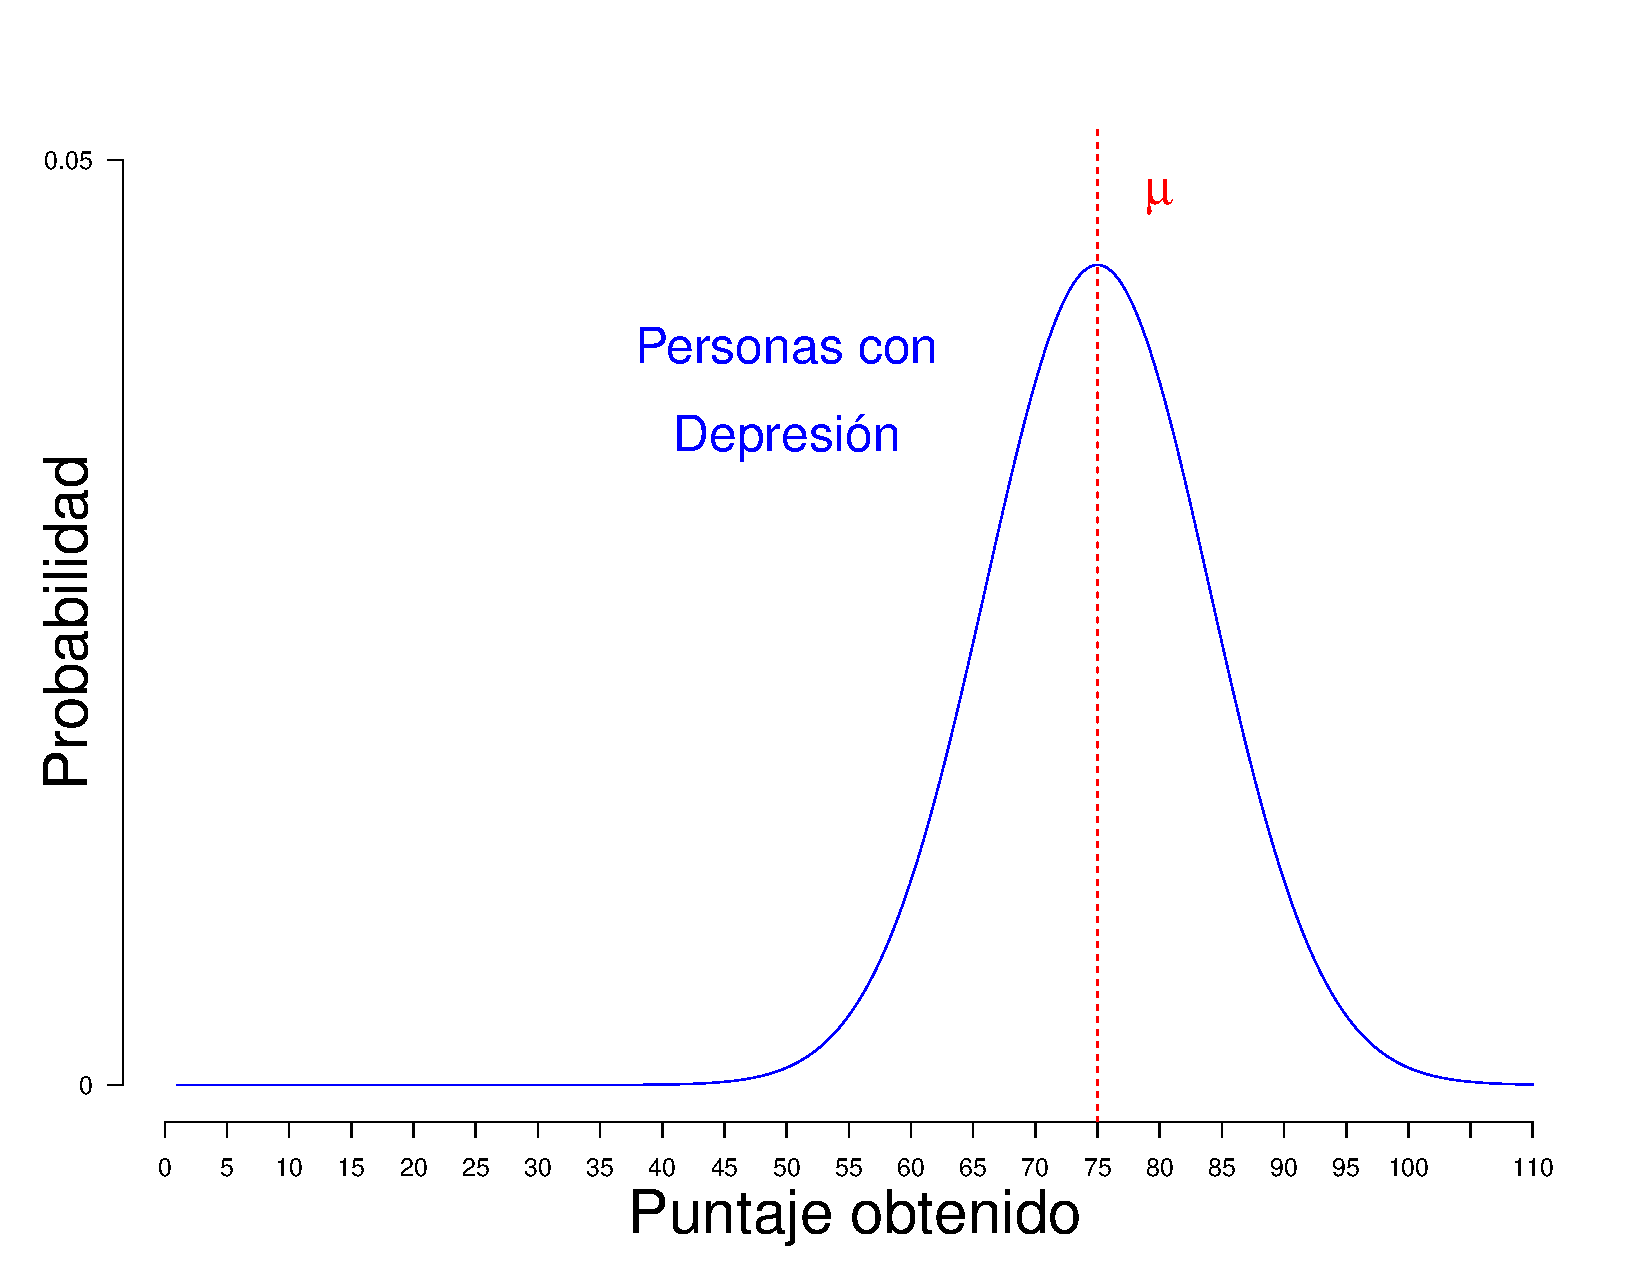
\includegraphics[width=0.75\textwidth]{Figures/Signal_Presentation} 
%\decoRule
\caption[Variabilidad en la presentación de los estímulos]{La variabilidad en la presentación de los estímulos es representada con una distribución de probabilidad normal: En una prueba clínica de Depresión, las personas que presentan dicha condición (la Señal) pueden obtener puntajes dentro de un rango de valores con mayor o menor probabilidad al rededor de una media ($\mu$, señalada en rojo). Los valores presentados son arbitrarios.}
\label{fig:Senal_presentacion}
\end{figure}

En general, las Figuras~\ref{fig:Senal_percepcion} y \ref{fig:Senal_presentacion} ilustran un elemento fundamental en la forma en que la SDT concibe la detección de señales como un problema de adaptabilidad: la variabilidad es intrínseca a la percepción de los estímulos, ya sea porque nuestros sistemas sensoriales no los capturan igual en cada presentación, o porque los estímulos no se nos presentan exactamente de la misma forma en cada ocasión. Es otras palabras, los estímulos en cuya detección están interesados los organismos (las señales) son intrínsecamente variables (Tanner y Swets, \citeyear{Tanner1954}).\\

\pagebreak

    \underline{b) La variabilidad en el Entorno: Ruido}\\

%La señal coexiste con el ruido y puede llegar a confundirse con el mismo.
Además del hecho de que existe variabilidad implícita en las señales a detectar, es necesario tomar en cuenta que estas coexisten en el mundo con otros estímulos o estados que -dada su propia variabilidad- pueden llegar a producir evidencia similar y confundir el diagnóstico de detección emitido por los organismos implicados en la tarea (Tanner y Swets, \citeyear{Tanner1954}). Esta misma idea fue propuesta por primera vez por Thurstone (\citeyear{Thurstone1927}), quien desarrolló un modelo estadístico para dar cuenta del problema que supone la discriminación entre dos estímulos, tomando en cuenta la variabilidad en la percepción y presentación de estos, una idea que posteriormente sería ampliamente desarrollada en Psicofísica (Swets, \citeyear{Swets1973}).\\

\begin{figure}[h]
\centering
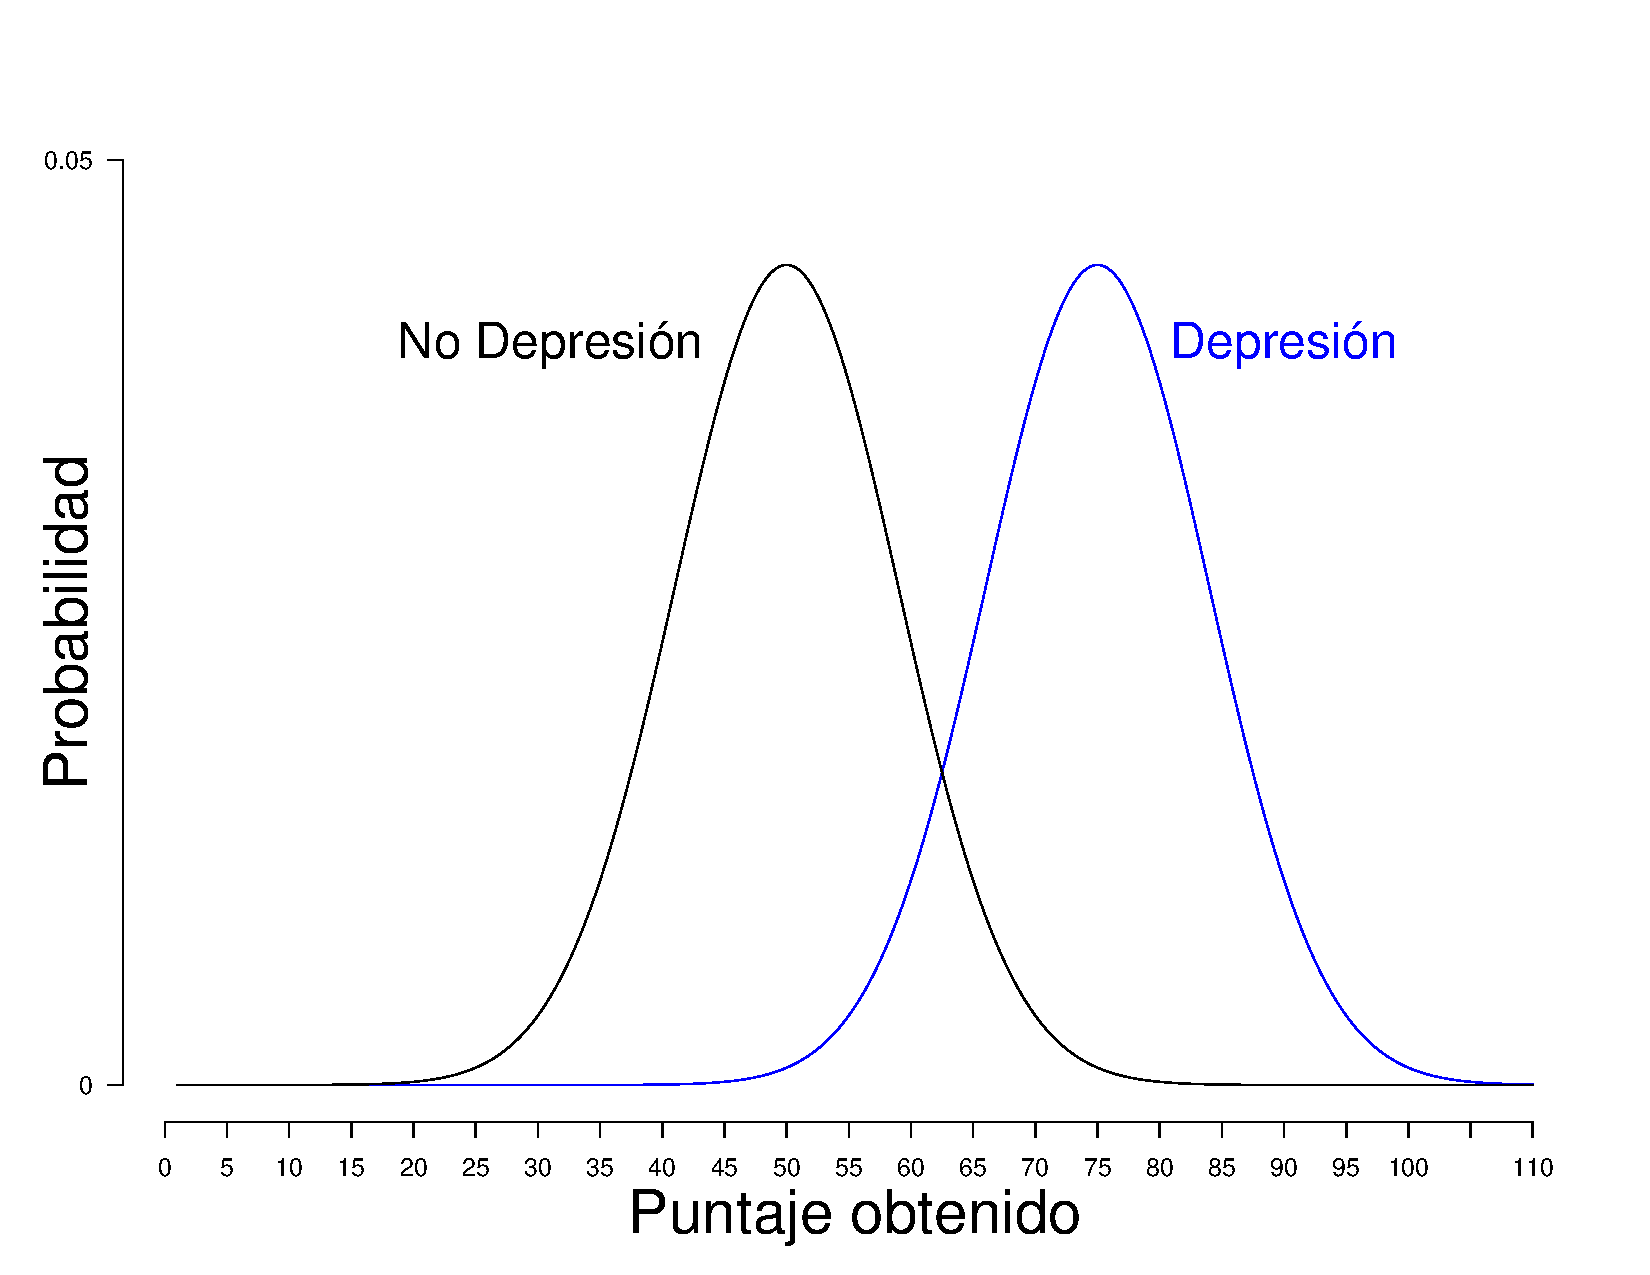
\includegraphics[width=0.75\textwidth]{Figures/Noise} 
%\decoRule
\caption[Variabilidad en la señal y en el ruido]{Extensión del ejemplo sobre la variabilidad en los puntajes obtenidos en una prueba clínica por pacientes con depresión, donde además de la distribución asociada a la señal (en azul), se añade una distribución que representa los puntajes registrados por personas que no tienen depresión (el ruido; en negro). El sobrelape entre ambas distribuciones ilustra la incertidumbre contenida en la tarea.}
\label{fig:Noise}
\end{figure}

Retomando el ejemplo ilustrado en la Figura~\ref{fig:Senal_presentacion} sobre la variabilidad en los puntajes obtenidos en una prueba clínica por personas con depresión, en la Figura~\ref{fig:Noise} se agrega un segundo punto clave en la concepción de la detección de señales como un problema de decisión: también existe variabilidad en los puntajes obtenidos por las personas que responden la prueba sin tener dicha condición, con su propia distribución de probabilidad (en color negro). Nótese que ahora existe un sub-rango de valores donde las dos distribuciones se sobrelapan y recordemos que el objetivo de aplicar estas pruebas es detectar -\textit{diagnosticar}- la depresión -la señal- con base en el resultado obtenido por el paciente evaluado, ¿Cuál sería el diagnóstico pertinente para una persona que obtuvo un puntaje dentro del área de sobrelape? De acuerdo con la SDT, la forma ideal de resolver este conflicto -asumiendo que se conocen las distribuciones que subyacen al desempeño de las personas con y sin depresión- es optar por el juicio de elección \texit{más probable} a la luz de los datos (es decir, el que tenga una mayor densidad de probabilidad a la altura del puntaje registrado). El problema es claro: en tanto que la señal y el ruido pueden llegar a producir la misma evidencia, los sistemas detectores no pueden tener certeza absoluta sobre el juicio de detección a emitir y en su lugar, deben elegir aquel que les permita optimizar su comportamiento.\\ 

En el marco de la SDT, la discriminabilidad en las tareas de detección se define mediante la proporción de evidencia que comparten la señal y el ruido (es decir, \textit{'¿qué tan probable es que la señal y el ruido se confundan?'}), y en términos de la representación gráfica propuesta por la SDT, implica una evaluación de qué tan grande es el área de sobrelape entre las distribuciones, volviéndose esta el reflejo directo de la incertidumbre contenida en la tarea (\textit{'¿Qué tan discriminable -diferente- es la señal respecto del ruido?'}).\\

\begin{figure}[h]
\centering
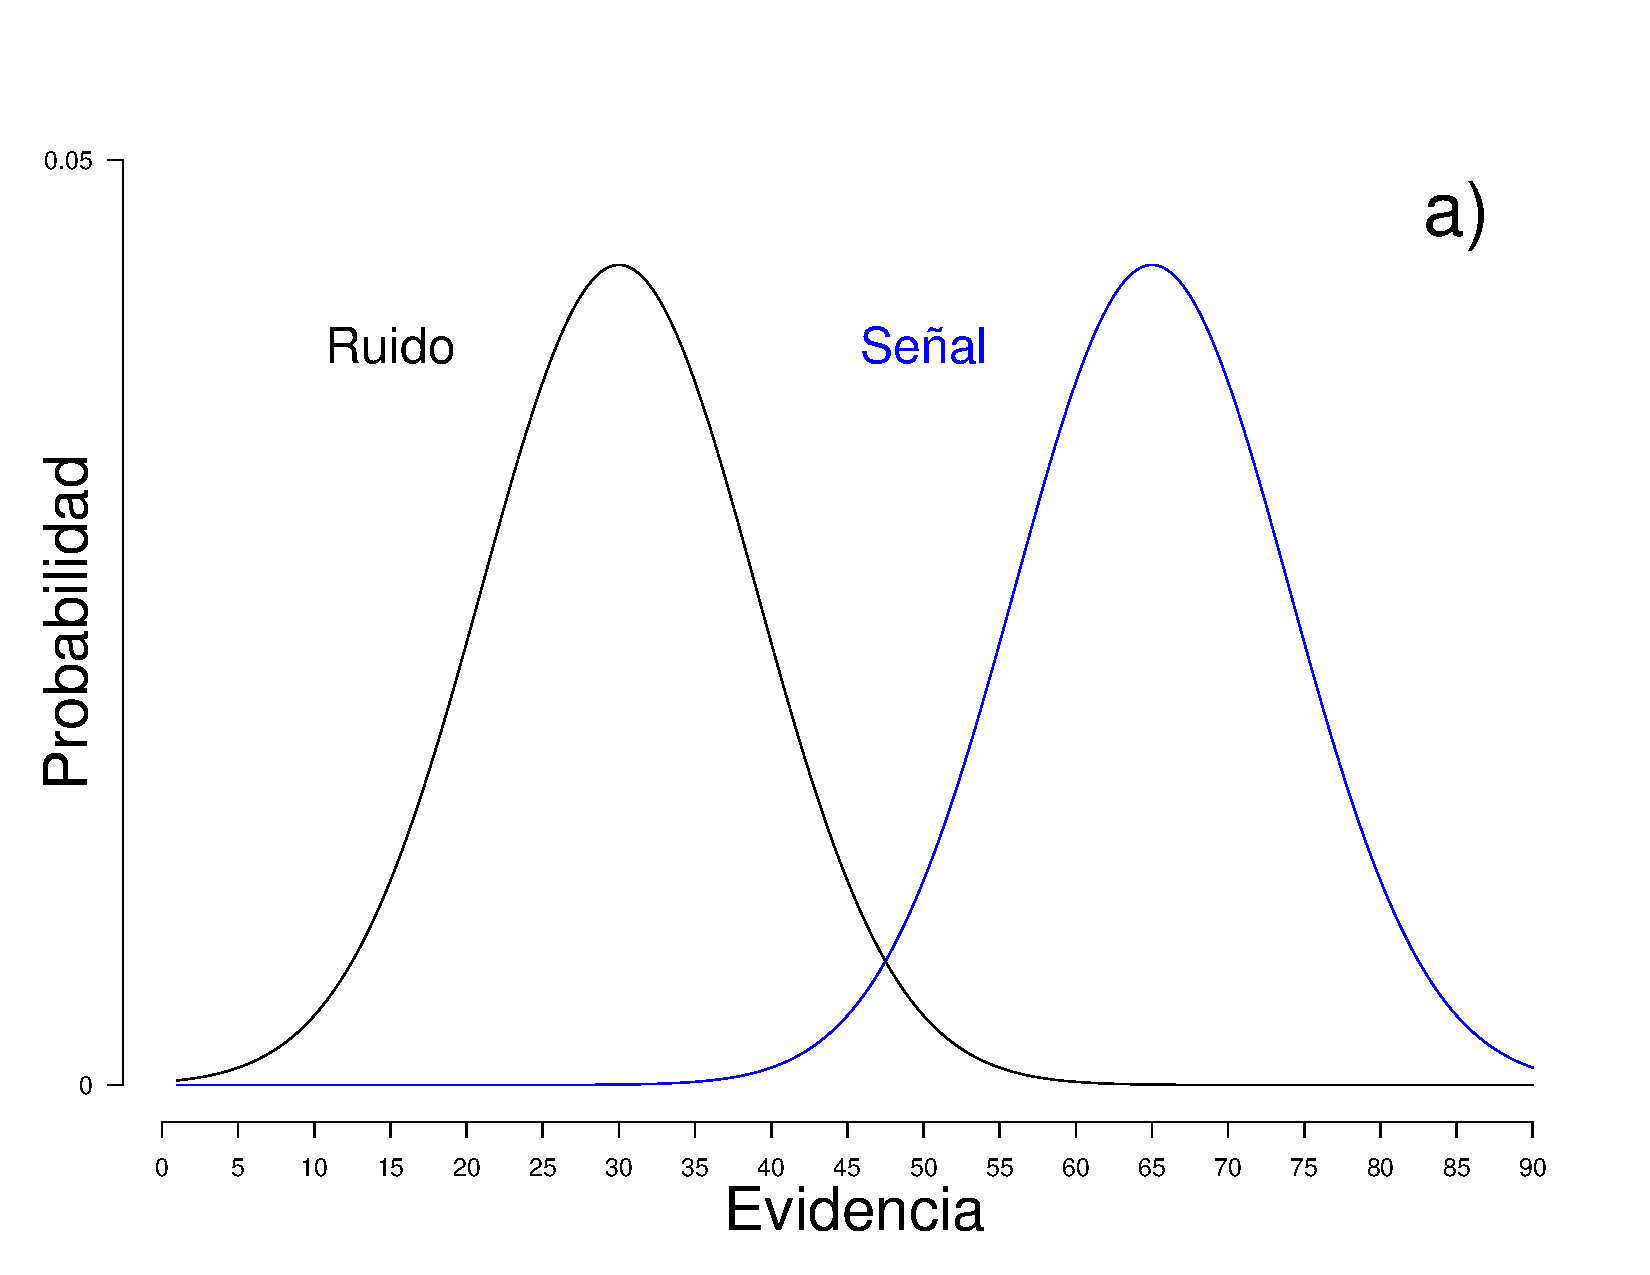
\includegraphics[width=0.65\textwidth]{Figures/Overlap_Small}\\ 
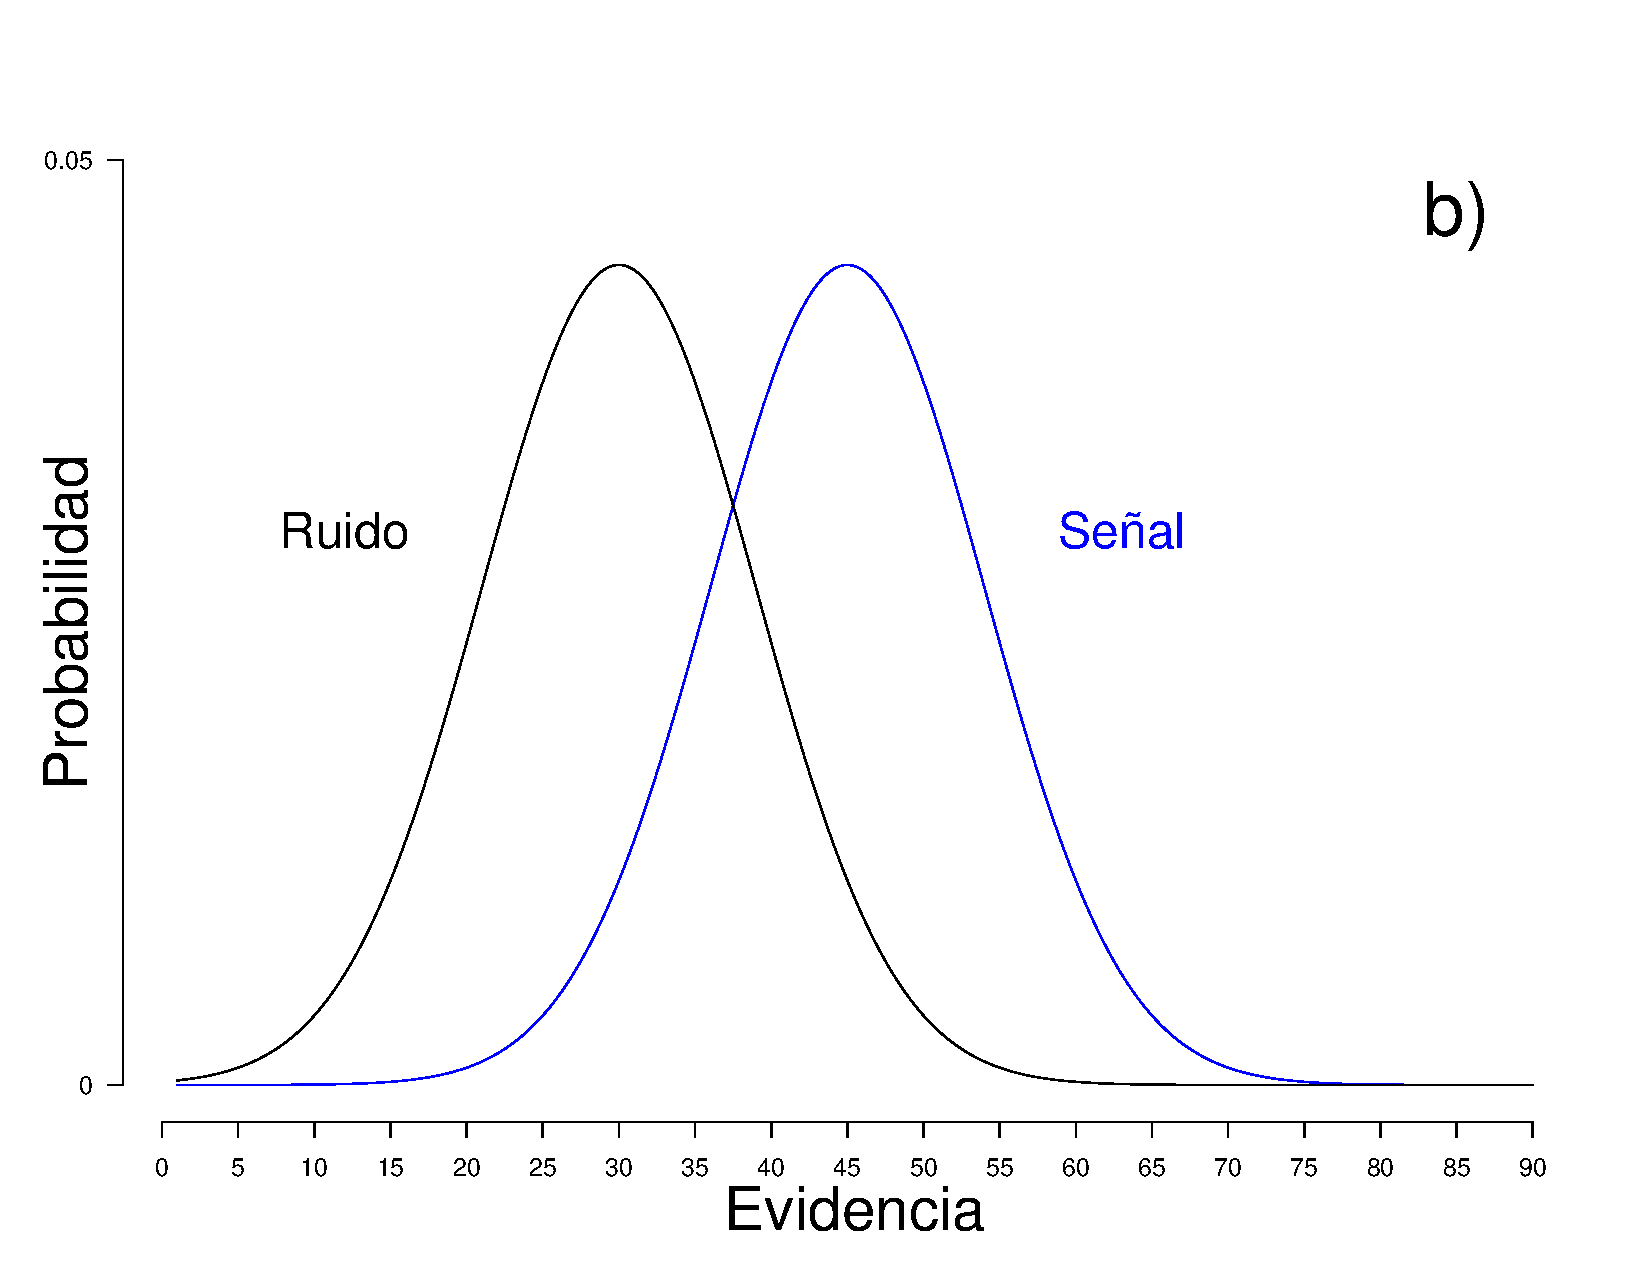
\includegraphics[width=0.65\textwidth]{Figures/Overlap_Big} 
%\decoRule
\caption[La detección como una tarea con incertidumbre: el sobrelape entre las distribuciones]{La distancia entre las distribuciones de ruido y señal determina el sobrelape entre las mismas y por tanto, la incertidumbre contenida en la tarea. En el panel a) las distribuciones aparecen muy separadas y se asume poca incertidumbre.  En el panel b) se presenta un escenaro con mayor incertidumbre, siendo que el sobrelape entre las distribuciones es mayor.}
\label{fig:Overlap}
\end{figure}

La Figura~\ref{fig:Overlap} presenta dos figuras representativas que ilustran la relación entre la distancia entre las distribuciones de Ruido y Señal -y el área de sobrelape entre estas- y su interpretación en términos de la discriminabilidad de los estímulos contenidos en la tarea. En el panel superior (a), las distribuciones están muy separadas y el sobrelape entre estas es pequeño, sugiriendo un entorno con poca incertidumbre donde es muy poco probable encontrar evidencia que pueda confundir al organismo -\textit{discriminabilidad alta}-. Por otro lado, si las distribuciones están más juntas, como ocurre en el panel inferior (b), el sobrelape será más grande y habrá un mayor rango de evidencia que se vincule simultáneamente con ambos estados del mundo, dificultando la emisión del juicio de detección adecuado -\textit{discriminabilidad baja}-.\\

La Discriminabilidad en una tarea de detección es producto de la variabilidad con que los posibles estados del mundo se presentan y perciben por los sistemas detectores. Es decir, depende tanto de las propiedades intrínsecas de los estímulos a evaluar -\textit{¿Qué tanto parecido tienen los estímulos con la señal y los estímulos sin esta?}- como de la precisión con que los sistemas detectores son capaces de discernir entre dichas instancias -\textit{¿Qué tan bueno es el organismo para distinguir una señal del ruido?}- (Nevin, \citeyear{Nevin1969}). Por ejemplo, no es lo mismo tratar de detectar una manzana entre un montón de naranjas que entre un montón de melocotones, (en general, esperaríamos que la tarea fuera más sencilla en el primer escenario al tener una mayor discriminabilidad); de la misma forma, la tarea de detectar si un instrumento musical está desafinado no es igual de difícil para un músico que para una persona sin educación musical.\\

  \textbf{2.- El papel del Sesgo: La detección es decisión}\\

La variabilidad en la presentación y percepción de los eventos en el mundo constituye el elemento clave para entender la detección de señales como una problema cargado de incertidumbre, donde no se puede confiar completamente en la evidencia presente para emitir un juicio de detección.\\

De acuerdo con la SDT, los organismos compensan la incertidumbre contenida en las tareas de detección con la información que poseen sobre el entorno que, en términos generales, puede ser de dos tipos: 1) información probabilística e 2) información sobre las consecuencias comprometidas (Nevin, \citeyear{Nevin1969}).\\

Como ejemplo, tomemos el caso de un médico que trata de decidir si los resultados obtenidos en cierta prueba clínica son evidencia suficiente para diagnosticar una enfermedad \textit{X} a un paciente \textit{Y}. La evidencia con la que el médico cuenta es imprecisa: toda prueba clínica tiene un margen de error y su lectura debe complementarse con información extraída de la historia clínica del paciente; el médico debe juzgar la evidencia en función de toda la información de la que dispone: \textit{¿Qué tan confiable es la prueba?} o \textit{¿Cuál es su tasa de aciertos y errores?}; \textit{¿Qué tan común es la enfermedad cuya presencia se intenta determinar?} y \textit{¿Qué tan probable es que el paciente Y tenga la enfermedad X?}; de acuerdo con su historia clínica, \textit{¿Qué tanto correlacionan sus características con los factores de riesgo asociados a la enfermedad?} y \textit{¿Qué tanto afecta eso la probabilidad de que Y tenga la enfermedad X?}. Y aún ponderando toda esta información, el problema no termina aquí. La información probabilística permite hacer inferencias sobre cuál es la conclusión más \textit{probable}, pero sigue sin haber certeza sobre el diagnóstico. Para optimizar su comportamiento y tomar la mejor decisión posible, el médico también debe tomar en consideración la información que posee sobre las consecuencias asociadas a cada escenario posible: a) Si el paciente tiene la enfermedad y el médico la detecta acertadamente, podrá tratarse a tiempo; b) Si tiene la enfermedad y el médico falla en detectarla, podría poner en riesgo su vida; c) Si no tiene la enfermedad y el médico le dice que sí, se gastarán recursos innecesarios en solucionar un problema que no existe, corriendo el riesgo de que el tratamiento le haga daño y d) Si no tiene la enfermedad y el médico decide no darle el diagnóstico, todo permanecerá igual. La tarea del médico es mucho más compleja de lo que parecía en un principio, puesto que no se limita a la lectura de la prueba clínica, sino que tiene que ponderar lo que sugieren los resultados de la misma con toda la información que posee sobre la probabilidad de las interpretaciones posibles y las consecuencias comprometidas.\\

\begin{figure}[h]
\centering
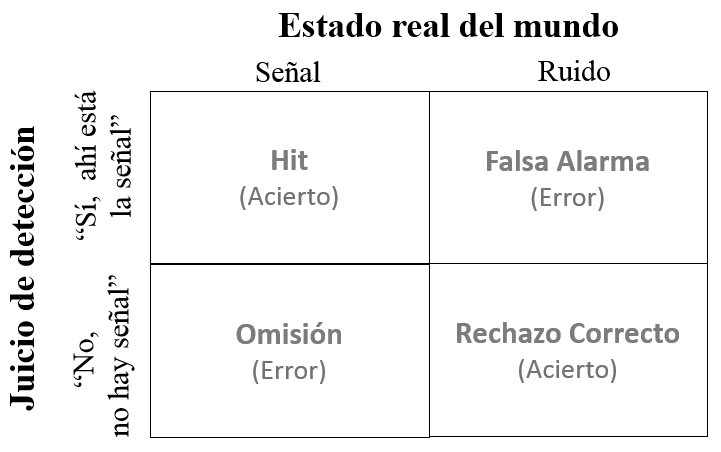
\includegraphics[width=0.75\textwidth]{Figures/Matriz_Outputs} 
%\decoRule
\caption[Matriz de contingencia: Resultados a obtener en una tarea de detección]{Los cuatro posibles resultados a obtener en una tarea de detección de señales, de acuerdo con la correspondencia entre el juicio emitido y el estado del mundo.}
\label{fig:Mat_Output}
\end{figure}

De acuerdo con la correspondencia entre el \textit{estado real del mundo} -la presencia o ausencia de la señal- y el juicio emitido por el sistema detector, la SDT distingue entre dos tipos de aciertos y errores, ilustrados en la Figura~\ref{fig:Mat_Output} con una Matriz de contingencia. Cuando la señal está presente el organismo puede detectarla adecuadamente (un \textbf{Hit}) o dejarla pasar (una \textbf{Omisión}); y si por el contrario, la señal no está presente, el organismo puede acertar al diagnosticar su ausencia (un \textbf{Rechazo correcto}) o confundir el ruido con la señal, (una \textbf{Falsa Alarma}).\\

La SDT asume que el organismo fija un criterio de elección para determinar a partir de cuánta evidencia va a juzgar la presencia de la señal, con base en la informació que posee sobre la probabilidad de que ésta ocurra y las consecuencias comprometidas en su detección (Tanner y Swets, \citeyear{Tanner1954}; Swets y cols., \citeyear{Swets1961}; Nevin, \citeyear{Nevin1969}). En términos de la representación gráfica del modelo, el criterio se concibe como una línea vertical que atraviesa las distribuciones de ruido y señal (como se ilustra en color rojo en la Figura~\ref{fig:Graf_Outputs}), para definir a partir de cuánta evidencia se emitirá un juicio de detección afirmativo.\\

La Figura~\ref{fig:Graf_Outputs} presenta la representación final de los problemas de detección bajo el marco de la SDT: se tienen dos distribuciones de probabilidad que representan la variabilidad con que la señal y el ruido ocurren en el ambiente y una línea roja que señala el criterio que el sistema detector va a utilizar para emitir sus juicios de detección. Como se ilustra con distintos colores en la figura, la localización del criterio determina la probabilidad con que el organismo podría incurrir en cada uno de los resultados expuestos previamente en la figura~\ref{fig:Mat_Output}.\\

\begin{figure}[bh]
\centering
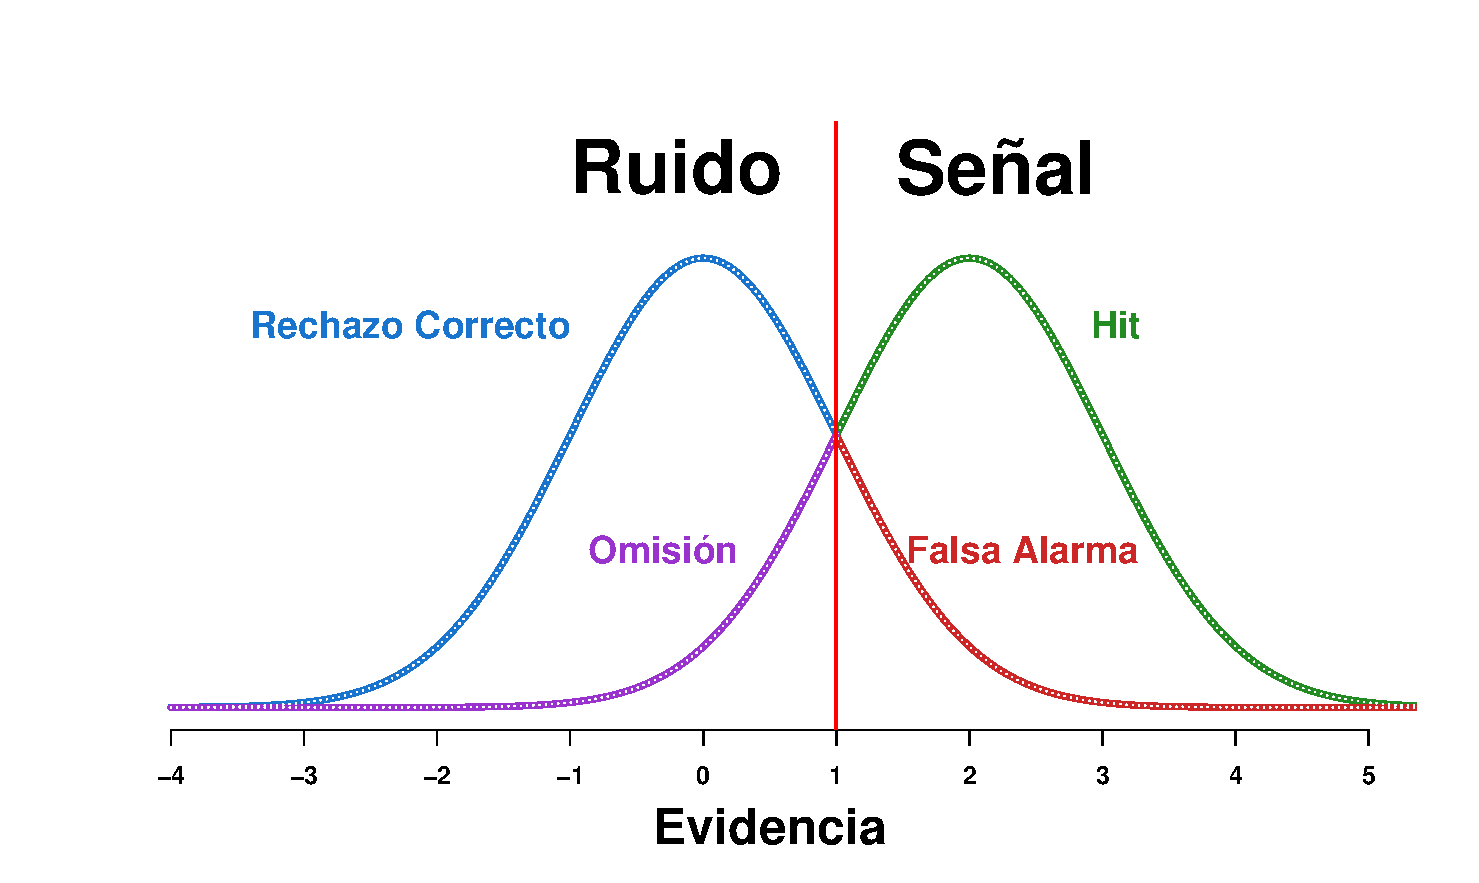
\includegraphics[width=0.8\textwidth]{Figures/SDT_OutcomesR} 
%\decoRule
\caption[Representación gráfica de las tareas de detección y los posibles resultados a obtener]{Representación gráfica del problema de detección de señales de acuerdo con la SDT: existen dos distribuciones de probabilidad que describen la variabilidad con que la señal y el ruido se presentan en el entorno, con un área de traslape que refleja la incertidumbre en la tarea. El criterio de elección fijado por el organismo (línea roja) determina a partir de cuánta evidencia se juzgará la presencia de la señal y define la probabilidad de cometer un acierto o error (en colores).}
\label{fig:Graf_Outputs}
\end{figure}

De acuerdo a la estructura de la tarea y al conocimiento que los organismo tengan sobre ella, es posible que se desarrolle un \textit{sesgo} de elección que lleve a favorecer -\textit{hacer más propensa}- la emisión de un juicio de detección particular (Nevin, \citeyear{Nevin1969}). De esta forma, la localización del criterio sobre el eje de evidencia es un reflejo directo de este sesgo, que puede variar en función de dos grandes factores:\\

      \underline{a) Los errores cuestan y los aciertos pagan: Matrices de pago}\\

La variabilidad asociada a los estímulos en el ambiente da pie a que los sistemas involucrados en tareas de detección de señales cometan errores. Tomando en cuenta que las señales son estímulos relevantes para el sistema, en tanto que permiten dirigir su comportamiento en función de las relaciones de contingencia anunciadas con su detección, acertar o errar en el juicio emitido tiene consecuencias importantes. Los aciertos pagan y los errores cuestan, y más aún, cada uno lo hace con distinta magnitud.\\

Imaginemos el caso de un conejo que tiene que decidir, tan rápido como pueda, si el sonido que acaba de escuchar en la maleza corresponde o no, con el de un depredador. La penalización por cometer una Falsa Alarma -un gasto innecesario de energía al correr por nada- es sustancialmente diferente al precio que tendría que pagar por una Omisión -¡la muerte!-. Dadas las consecuencias en juego, es muy probable que el conejo emita un juicio de detección afirmativo (\textit{'¡Sí, es un depredador!'}) y corra por su vida, aún con muy poca evidencia.\\

\begin{figure}[h]
\centering
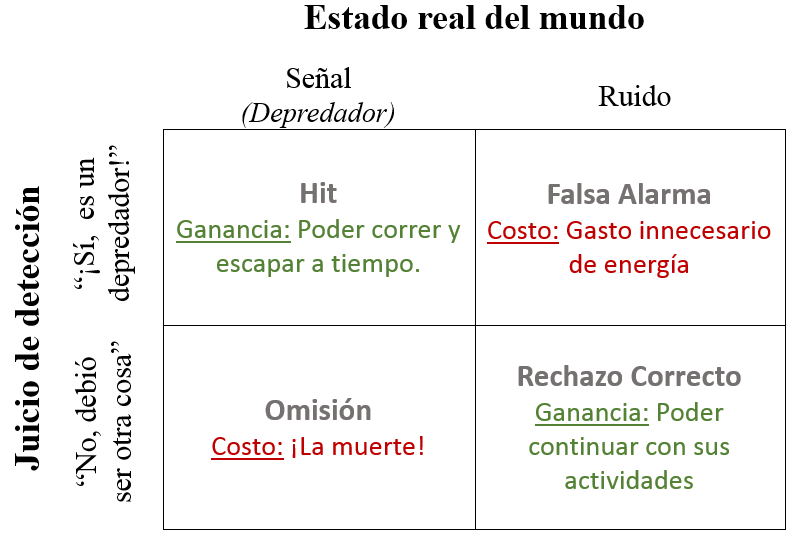
\includegraphics[width=0.80\textwidth]{Figures/Matriz_Pagos} 
%\decoRule
\caption[Matriz de Pagos: Consecuencias comprometidas en una tarea de detección hipotética (ejemplo)]{Matriz de pagos con los costos y ganancias comprometidos en la tarea de detectar un depredador.}
\label{fig:Mat_Pagos}
\end{figure}

La figura~\ref{fig:Mat_Pagos} presenta lo que en los modelos clásicos de decisión se conoce como \textit{Matriz de Pagos} y que se utiliza para señalar, de acuerdo a una matriz de contingencia, los costos y ganancias asociados con las tareas de detección. De acuerdo con la SDT, ya que no se puede tener certeza absoluta sobre el juicios de detección a emitir, la evidencia es juzgada en función a un criterio de elección que toma en cuenta las consecuencias comprometidas en su entorno, para guiar de manera óptima el comportamiento del organismo (Killeen, \citeyear{Killeen2014}).\\

      \underline{b) Estimados de Probabilidad}\\

Los organismos inmersos en tareas de detección tienen expectativas sobre la probabilidad de observar una señal en su entorno. Ya sea como resultado de su experiencia directa con el mundo, o porque es información que les ha sido proporcionada de manera externa (Nevin, \citeyear{Nevin1969}), los agentes detectores tienen alguna idea o conocimiento sobre la estructura probabilística de la tarea a resolver, en dos sentidos: 

\begin{itemize}
\item \textsl{Un estimado prior.} Con independencia de cuál sea la evidencia evaluada de manera inmediata, \textit{¿Qué tan probable es encontrar la señal en esta situación particular?}\\

Si los organismos se encuentran en un entorno donde saben que es prácticamente imposible encontrar la señal, es muy probable que decidan descartar la evidencia que se les presente aún cuando correlacione con lo que se esperaría de una señal. Recordemos el ejemplo planteado anteriormente sobre el querer determinar la edad de una persona con la que hablamos por teléfono: si la llamada fue hecha a un despacho de abogados -o cualquier otro escenario donde se piense que es muy poco probable encontrar a un niño-, y la persona al otro lado del teléfono tiene una voz muy aguda, es muy poco probable que se decida pensar \textit{'Oh, estoy hablando con un niño'}.\\

\item \textsl{La verosimilitud.} Dado lo que se sabe sobre cómo se presentan los estímulos en el entorno, \textit{¿qué tan verosímil es la evidencia?} o bien, \textit{¿qué tan probable es que la señal se presente con la evidencia presente?}\\

Una vez que los organismos han adquirido información suficiente sobre su entorno -o una tarea particular- y conocen la variabilidad con que la señal y el ruido aparecen, los juicios de detección pueden ser emitidos a partir del cómputo de una razón de verosimilitud que permita al organismo estimar cuál es el estado del mundo con que la evidencia incierta se relaciona con mayor probabilidad. Es decir que, en términos de la representación gráfica del modelo, se asume que cuando los organismos se enfrentan a evidencia que cae en el área de sobrelape entre las distribuciones, optarían por elegir el juicio de detección que corresponda con la distribución que tenga una mayor densidad de probabilidad (es decir, la distribución que sea más alta en ese punto particular del eje de decisión) (Nevin, \citeyear{Nevin1969}).\\
\end{itemize}

De contar con un estimado prior y un buen conocimiento sobre las funciones de verosimilitud, es posible suponer que los organismos opten por el juicio de detección que resulte más probable, con base en el cómputo de una inferencia bayesiana (Ma, \citeyear{WeijiMa}; Ma, Kording y Goldreich \citeyear{WeijiMa2012}; Pouget, BEck, Ma y Latham, \citeyear{Pouget2013}).\\

\subsection{Parámetros del modelo}\\

La SDT, además de proporcionar un modelo estadístico para comprender las implicaciones adaptativas de los problemas de detección, funge como una herramienta que -dados los supuestos que hace sobre este tipo de tareas- permite hacer estimaciones sobre la discriminabilidad y el sesgo de sistemas inmersos en tareas de detección experimentales (Stainslaw y Todorov, \citeyear{Stainslaw1999}; McNicol, \citeyear{McNicol1}).\\

Las tareas de detección diseñadas en el laboratorio suelen estar compuestas por un amplio número de ensayos, a lo largo de los cuales se presenta aleatoriamente la señal o el ruido y se les solicita a los participantes que emitan un juicio de detección. Dependiendo el objetivo del estudio realizado, se pueden implementar manipulaciones adicionales (Nevin, \citeyear{Nevin1969}), o utilizar distintos protocolos en la presentación de la tarea de detección, (descritos en detalle en la \textbf{Sección 2.1.3}; McNicol, \citeyear{McNicol2}).\\

Al someter un sistema a una misma tarea de detección en repetidas ocasiones (como ocurre en las tareas experimentales), se espera encontrar variabilidad en los resultados obtenidos: el sistema no acertará o errará siempre, la evidencia evaluada no rebasará el criterio de elección en todos los ensayos a causa de la variabilidad en los estímulos (Wickens, \citeyear{Wickens1}. A partir del número de aciertos y errores cometidos en los ensayos con Ruido y Señal, se computan las tasas con que se obtuvieron cada uno de los resultados posibles. Dentro del total de veces que se presentó la señal, se identifica cuántas veces se cometió un Hit o una Omisión, y dentro del total de veces que se presetó sólo el Ruido, la proporción de ensayos en que el participante hizo un Rechazo correcto o una Falsa alarma.\\

De acuerdo con la SDT clásica, las tasas de ejecución computadas en una tarea de detección son reflejo del área de las distribuciones de Ruido y Señal que caen a cada lado del criterio y pueden, por lo tanto, utilizarse para hacer inferencias sobre la localización del mismo, la distancia entre las distribuciones y la preferencia que podría tener el sistema por emitir una respuesta sobre otra (Wickens, \citeyear{Wickens1}; McNicol, \citeyear{McNicol1}; Gesheider, \citeyear{Gescheider}). A continuación, revisaremos en detalle cuáles son los parámetros incluidos en el modelo de detección de señales, cómo se calculan y qué información arrojan sobre la ejecución de los participantes.\\

  \textbf{Supuestos formales}\\

La estimación paramétrica del modelo de detección de señales se desarrolla en torno a una serie de supuestos formales -especificaciones técnicas- que facilitan la interpretación de los datos obtenidos a la luz de la representación gráfica propuesta por la SDT (Wickens, \citeyear{Wickens1}; Gescheider, \citeyear{Gescheider}; Stainslaw y Todorov, \citeyear{Stainslaw1999}).\\ 

\begin{enumerate}

\item  Dado que las cuatro tasas de ejecución se computan en función a dos conjuntos -total de estímulos con Señal y Ruido-, sólo se necesita de un par de ellas para tener información completa sobre el desempeño de los participantes. Por ejemplo, por consenso general suelen reportarse sólo las tasas de Hits y Falsas Alarmas -los aciertos y errores obtenidos cuando el participante respondió \textit{'Sí, detecto la señal'}-, pues las tasas de Omisiones y Rechazos correctos no son más que su complemento (Wickens, \citeyear{Wickens1}.\\

\item En su forma clásica, la SDT asume que las distribuciones de Ruido y Señal son distribuciones normales equivariantes (Stainslaw y Todorov, \citeyear{Stainslaw1999}).\\
  \begin{itemize}
  \item Se utilizan distribuciones normales como el \textit{default} para describir la variabilidad contenida en cualquier conjunto de estímulos Señal y Ruido, pero existe literatura que explora la conveniencia de representar la incertidumbre con otro tipo de distribuciones (Wickens, \citeyear{Wickens1}; Ma, \citeyear{WeijiMa2009}).\\
  \item En la mayoría de sus aplicaciones, se asume que las distribuciones de ruido y señal comparten una varianza de 1 (Tanner y Swets, \citeyear{Tanner1954}). No obstante, al aplicar la SDT al estudio de la memoria de reconocimiento, se ha encontrado evidencia consistente de que la distribución de señal tiene una varianza mayor que la del ruido (Wixted, \citeyear{Wixted2007}).\\
  \end{itemize}

\item Se asigna de manera arbitraria una media en 0 a la distribución de Ruido para facilitar el cómputo del resto de los parámetros, utilizando ésta como punto de referencia (Wickens, \citeyear{Wickens1}; \citeyear{Gescheider}).\\

\item Una de las implicaciones directas de la forma en que está constituida la SDT es que, sea cual sea la evidencia con base en la cual se estén formando los juicios de detección -los valores en el eje $X$ sobre el que se despliegan las distribuciones-, se espera que la señal tenga \textit{más} de ello que el ruido, en tanto que este último implica su ausencia (Stainslaw y Todorov, \citeyear{Stainslaw1999}).\\
  \begin{itemize}

  \item La tasa de Falsas Alarmas no puede ser más grande que la tasa de Hits. Esto implicaría que hay una mayor área de la distribución de ruido por encima del criterio que de la distribución de señal. Esto, a su vez, sugeriría que el ruido cae por encima de la señal y se estaría violando el supuesto fundamental de que la Señal -la presencia de lo que queremos detectar- contiene más información que el Ruido -su ausencia-.\\
  \end{itemize}
\end{enumerate}

Los parámetros contemplados por el modelo evalúan el desempeño de los participantes en términos de los dos grandes factores que se asocian con la emisión de juicios de detección: la discriminabilidad y el sesgo. La aplicación exitosa de la SDT al estudio de una amplia gama de tareas de detección -que pueden variar desde el tipo de estímulos utilizados hasta el dominio o fenómeno a estudiar- es posible gracias a la abstracción de sus elementos. Los valores y el tipo de evidencia específicos sobre los cuales se despliegan las distribuciones de Ruido y Señal no importan tanto -de hecho, no suelen tomarse en cuenta en lo absoluto- como saber qué tanto sobrelape hay entre las distribuciones y cuál es el juicio de detección que se prefiere emitir.\\

\begin{itemize}
\item \underline{Criterio ($k$)}\\

La localización del criterio sobre el eje de decisión se puede computar de manera directa a partir de la tasa registrada de rechazos correctos, tomando como referencia la media asignada a la distribución de ruido ($0$). \\

El parámetro $k$ representa la localización del criterio sobre el eje de evidencia en unidades de \textit{desviación estándar} (Tanner y Swets, \citeyear{Tanner1954}). Su cómputo requiere interpretar la tasa de Falsas Alarmas como reflejo de la probabilidad acumulada -el área bajo la curva- por encima del criterio en la distribución de Ruido, siendo la tasa de Rechazos Correctos su complemento. Dado que la distribucion de ruido tiene media en 0 y desviación estándar de 1, la tasa de Rechazos Correctos (ó $1 - Tasa$ $de$ $Falsas$ $Alarmas$) puede ser transformada en \textit{Puntajes Z} para conocer la localización del criterio de elección sobre la distribución de ruido. Esto se realiza a partir del uso de la funcón matemática $\phi^{-1}$ (\textit{'phi inversa'}), que permite estimar conocer cuál es el puntaje Z que corresponde con el punto donde se ha acumulado cierta densidad de probabilidad en una distribución normal estándar, (Stainslaw y Todorov, \citeyear{Stainslaw1999}).\\

\begin{figure}[h]
\centering
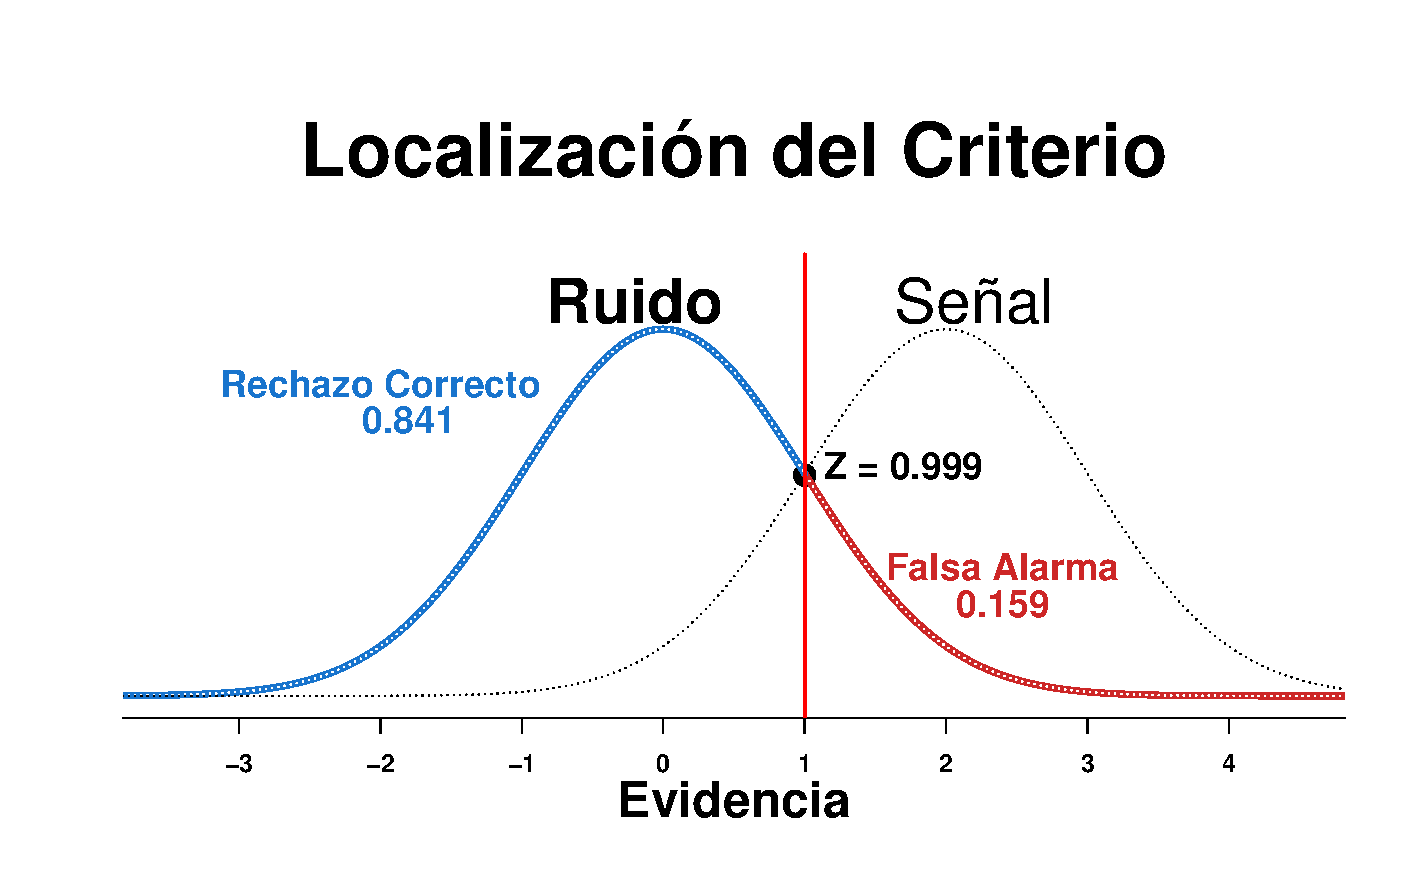
\includegraphics[width=0.75\textwidth]{Figures/Graficador_CriterioR} 
%\decoRule
\caption[Estimación paramétrica: La localización del criterio]{Estimación de la localización del criterio sobre el eje de decisión con base en las tasas de Falsas Alarmas y Rechazos Correctos.}
\label{fig:Graf_Criterio}
\end{figure}

La Figura~\ref{fig:Graf_Criterio} ilustra la estimación de $k$ a partir de las tasas de Falsas Alarmas y Rechazos Correctos. Al transformar esta última en Puntajes Z, se puede establecer la ubicación del criterio respecto del 0 de referencia planteado por la media de la distribución de ruido (Stainslaw y Todorov, \citeyear{Stainslaw1999}). Es decir:\\

\begin{center}
$k = PuntajeZ(Tasa$ $de$ $Rechazos$ $Correctos)$\\
\end{center}

\item \underline{Discriminabilidad ($d'$)}\\

La discriminabilidad de los estímulos comprometidos en una tarea de detección se cuantifica con un parámetro $d'$ que representa la distancia entre las medias de las distribuciones de ruido y señal, (Tanner y Swets, \citeyear{Tanner1954}). Dado que la distribución de ruido tiene media en 0, $d'$ también suele utilizarse para referir la ubicación de la media de la distribución de señal sobre el eje de evidencia, (McNicol, \citeyear{McNicol1}).\\ 

Una vez definida la localización del criterio relativa a la media de la distribución de ruido, es sencillo concebir el cómputo de $d'$ como una extensión de dicho procedimiento. Las tasas de Hits y Omisiones son utilizadas para establecer la localización de la media de la distribución de Señal sobre el eje de evidencia, a partir del criterio.\\ 

\begin{figure}[p]
\centering
%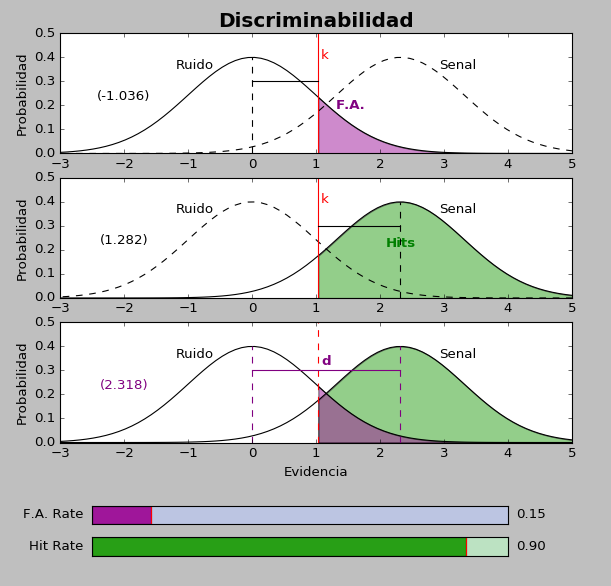
\includegraphics[width=0.80\textwidth]{Figures/Graficador_Discriminabilidad} 
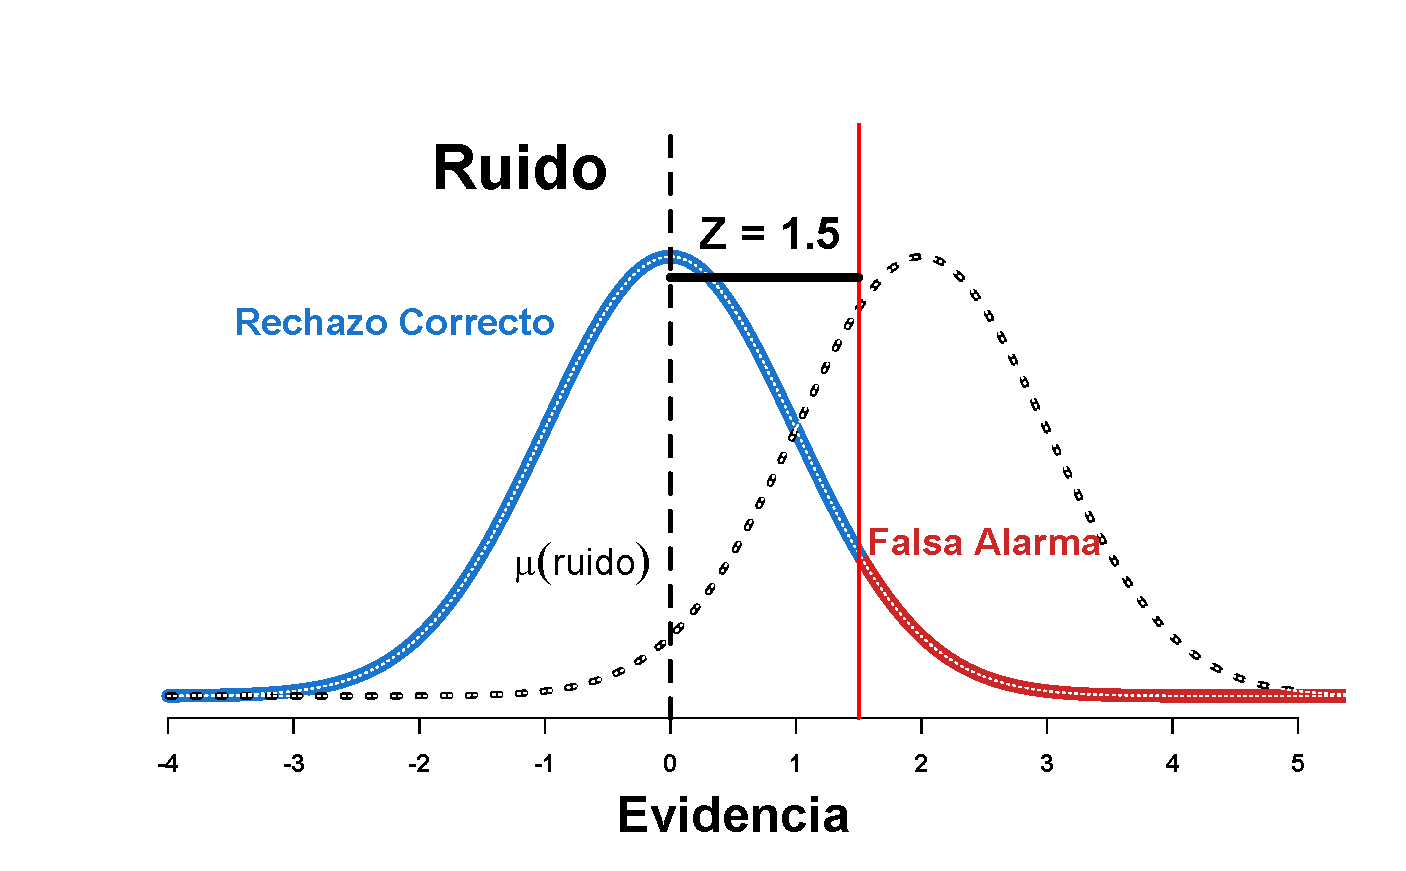
\includegraphics[width=0.70\textwidth]{Figures/dR_1}\\ 
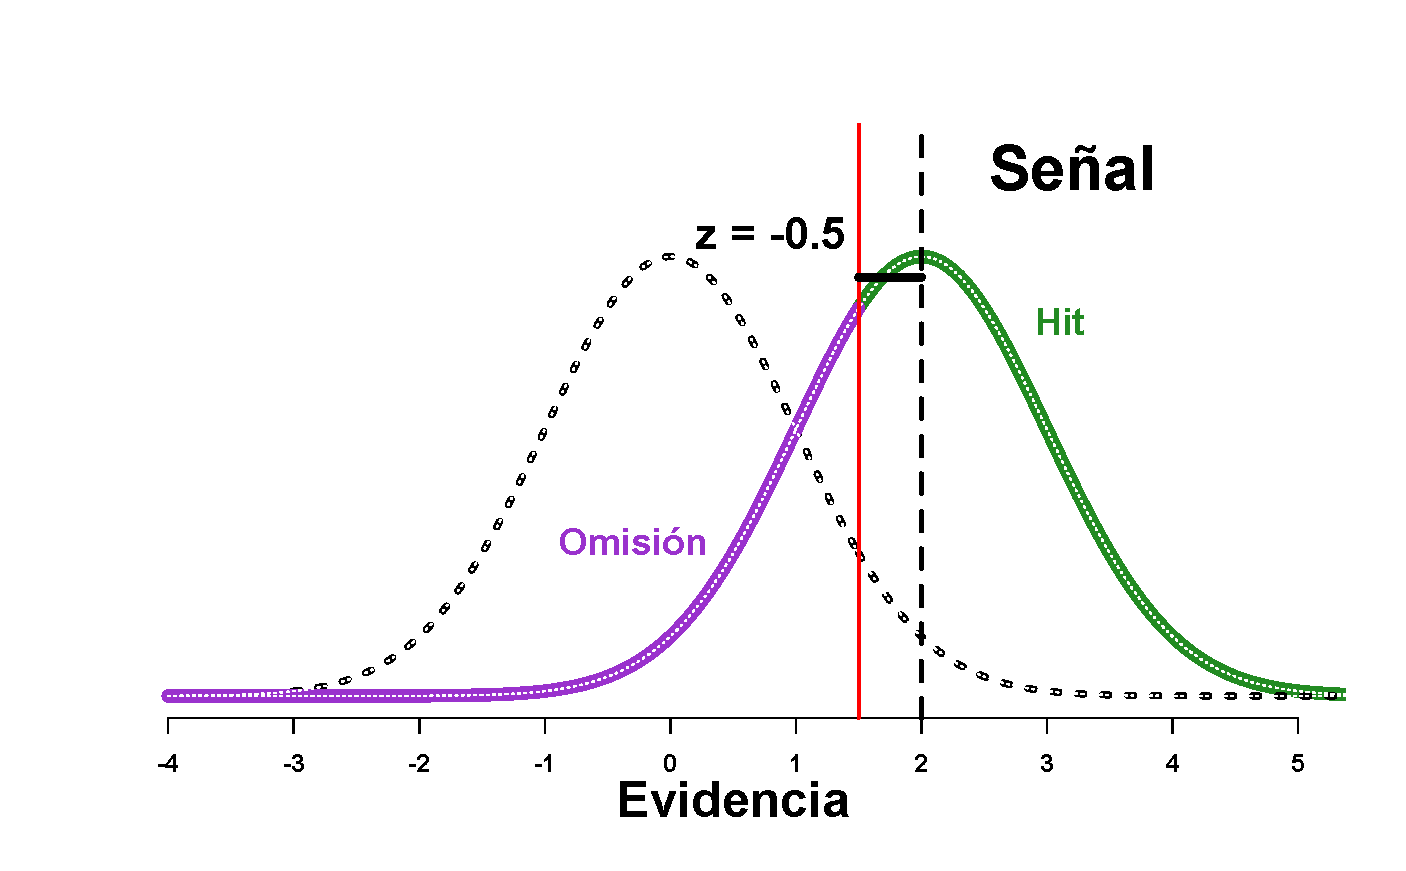
\includegraphics[width=0.70\textwidth]{Figures/dR_2}\\
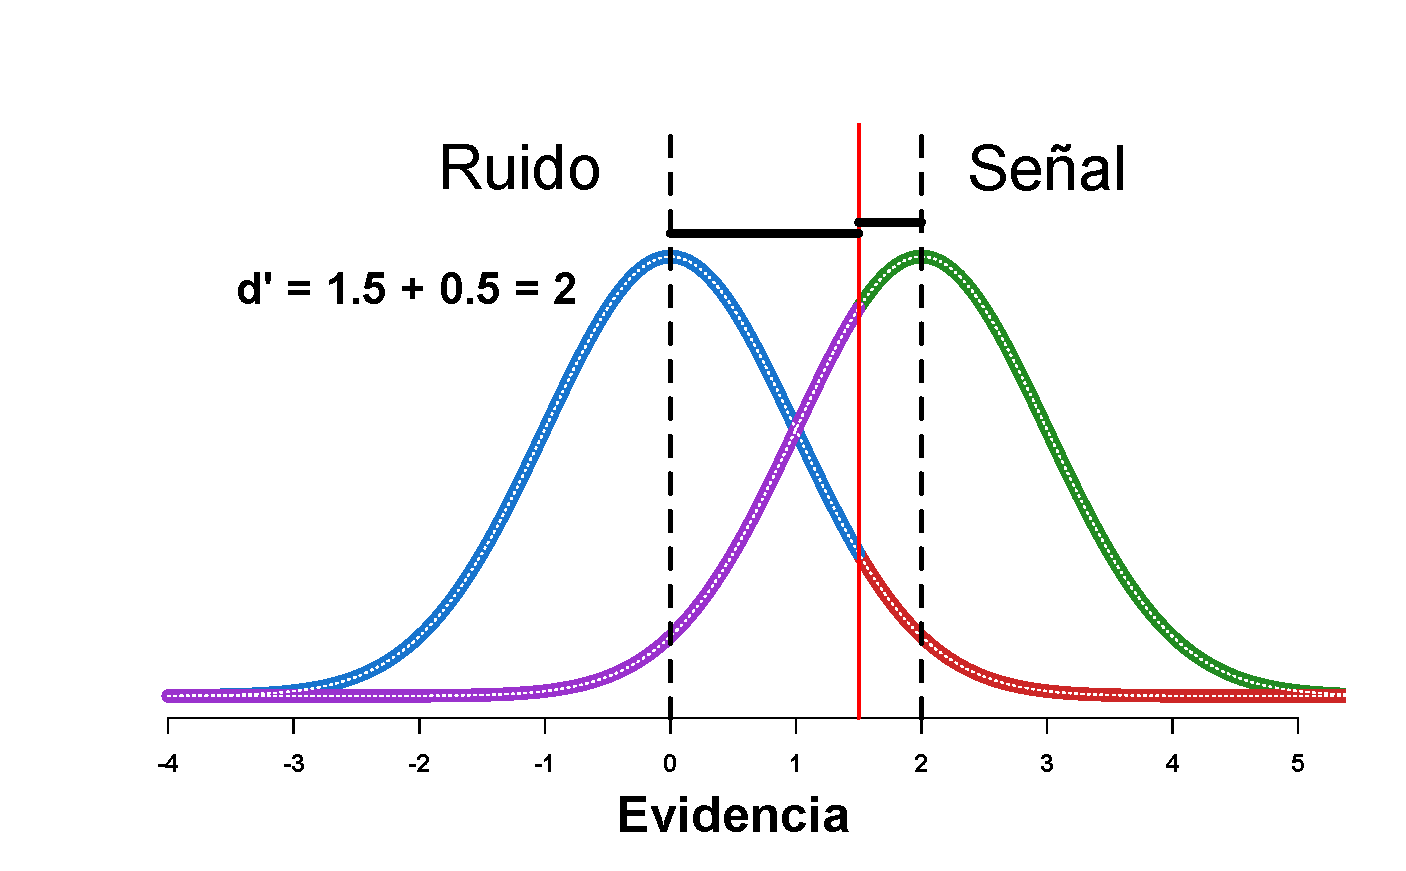
\includegraphics[width=0.70\textwidth]{Figures/dR_3}\\ 
%\decoRule
\caption[Estimación paramétrica: la discriminabilidad ($d'$)]{Ilustración del cómputo de $d'$. Las tasas de Falsas Alarmas y Rechazos correctos señalan la distancia entre el criterio y la media de la distribución de ruido (panel superior). Las tasas de Hits y Omisiones indican la distancia entre el criterio y la media de la distribución de Señal (panel intermedio). $d'$ se computa como la suma de las distancias entre el criterio y ambas medias.}
\label{fig:Graf_Discrim}
\end{figure}

La Figura~\ref{fig:Graf_Discrim} ilustra la secuencia lógica de pasos que guían el cómputo de $d'$:\\

\begin{enumerate}
\item En el panel superior, la tasa de Rechazos Correctos (señalada en color rojo) es convertida a Puntajes Z para conocer la distancia entre la media de la distribución de ruido y el criterio.\\

\item En el panel intermedio, se computa el puntaje Z que corresponde a la tasa de Omisiones ($1- Tasa$ $de$ $Hits$; señalada en color púrpura). En este caso, como el criterio cruza la distribución de señal por debajo de su media, se obtiene un puntaje Z negativo.\\

\item Finalmente, en el panel se ilustra el cómputo de $d'$: la distancia entre el criterio y cada una de las medias de las distribuciones de ruido y señal se suma. Es decir:\\

\begin{center}
$d' = PuntajeZ(1 - Tasa$ $de$ $Falsas$ $Alarmas) - PuntajeZ(1 - Tasa$ $de$ $Hits)$\\
donde el segundo término ($PuntajeZ(1 - Tasa$ $de$ $Hits)$), al tener un valor negativo, transforma la resta en una suma.\\
\end{center}

\end{enumerate}

El parámetro $d’$ sólo puede tener valores positivos ya que la distribución de señal siempre se situará por encima de la distribución de ruido, (Stainslaw y Todorov, \citeyear{Stainslaw1999}). La magnitud de la $d'$ computada es un reflejo de la discriminabilidad entre los estímulos que componen la tarea -la distancia entre las distribuciones que describen su variabilidad-. Si $d' = 0$, querría decir que las distribuciones de Ruido y Señal están completamente sobrelapadas y es imposible distinguir entre ellas (\textit{'No son discriminables en lo absoluto'}). \\

\item \underline{Sesgo ($\beta$ y $C$)}\\

La SDT cuenta con dos parámetros que permiten evaluar la magnitud y la dirección del sesgo con que se está respondiendo a la tarea (Stainslaw y Todorov, \citeyear{Stainslaw1999}; Macmillan y Creelman, \citeyear{Macmillan1996}).\\

\begin{itemize}
\item \underline{$\beta$}\\

El parámetro más comúnmente reportado en la literatura es Beta ($\beta$), que describe la razón entre la densidad de probabilidad de las distribuciones de señal y ruido a la altura del criterio: \\

\begin{center}
$\beta = \frac{p(Signal)}{p(Noise)}$ \\
\end{center}

En otras palabras, $\beta$ responde a la pregunta \textit{'¿Cuántas veces es más probable que la evidencia que corresponde con la localización del criterio sea una señal y no ruido?'}.

\item \underline{$C$}\\

Un segundo parámetro para computar el sesgo es $C$, que representa la distancia entre la localización del criterio utilizado por el sistema evaluado y el punto de intersección entre las distribuciones ($\frac{d'}{2}$):\\

\begin{center}
$C =  K - \frac{d'}{2}$ \\
\end{center}

Se utiliza $\frac{d'}{2}$ como punto de referencia para evaluar el sesgo del sistema porque se asume que esta debería ser la localización del criterio a utilizar por un sistema sin sesgo, pues el área de las distribuciones que cae por encima y por debajo de este punto es la misma. En otras palabras, un criterio en $\frac{d'}{2}$ llevaría a que existiera la misma probabilidad de cometer cualquier tipo de acierto y error.\\

El parámetro $C$ responde a la pregunta \textit{'¿Cuánto se aleja el criterio utilizado por el sistema de lo que se esperaría de un sistema sin sesgo?'}.\\

\end{itemize}

El sesgo puede ser evaluado en términos de dos factores: 1) ¿Qué tan sesgado está el sistema? y 2) ¿Cuál es el juicio de detección que se está favoreciendo?\\

El parámetro $\beta$ indica cuántas veces es más probable que la evidencia observada a la altura del criterio corresponda con la señal. Valores de $\beta$ por encima de 1, sugieren que el criterio choca con la distribución de señal en un punto más alto que la distribución de ruido; es decir, el sistema detector no emite juicios afirmativos hasta que existe una probabilidad alta de que la evidencia evaluada sea una señal, emitiendo con mayor probabilidad juicios negativos. Por otro lado, valores de $\beta$ entre 0 y 1 sugieren que es más probable que la evidencia encontrada a la altura del criterio provengan de la distribución de ruido, indicando que el sistema detector emite juicios afirmativos aún cuando es más probable que la evidencia observada no sea una señal. Finalmente, si el criterio del sistema cae sobre el punto de sesgo neutro ya descrito ($\frac{d'}{2}$), $\beta$ tendrá un valor de 1, pues el criterio tocaría ambas distribuciones a la misma altura.\\

Por su parte, el valor absoluto del parámetro $C$ proporciona información sobre la magnitud del sesgo con que el agente detector está favoreciendo la emisión de un juicio sobre el otro. La dirección del sesgo se puede determinar, dependiendo de si $C$ tiene un valor positivo o negativo. Si $C$ es negativo, quiere decir que $k < \frac{d'}{2}$; es decir, que el criterio se sitúa a la izquierda del punto neutro y promueve una mayor cantidad de respuestas afirmativas. Si $C$ es positivo, quiere decir que $k > \frac{d'}{2}$ y, por el contrario, se prefiere emitir juicios negativos.\\

\begin{figure}[h]
\centering
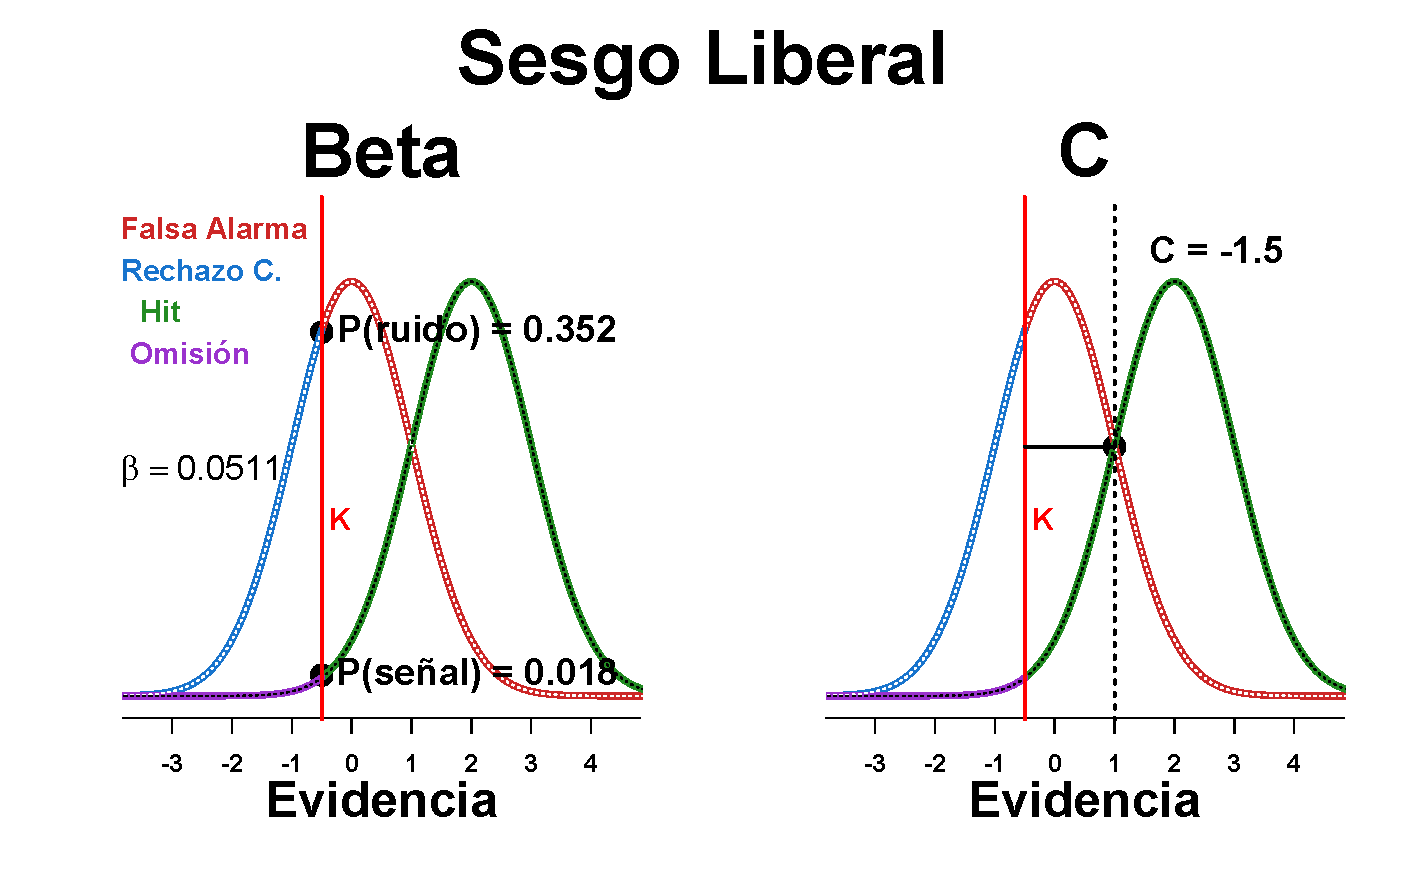
\includegraphics[width=0.8\textwidth]{Figures/Graficador_Sesgo_LiberalR}\\
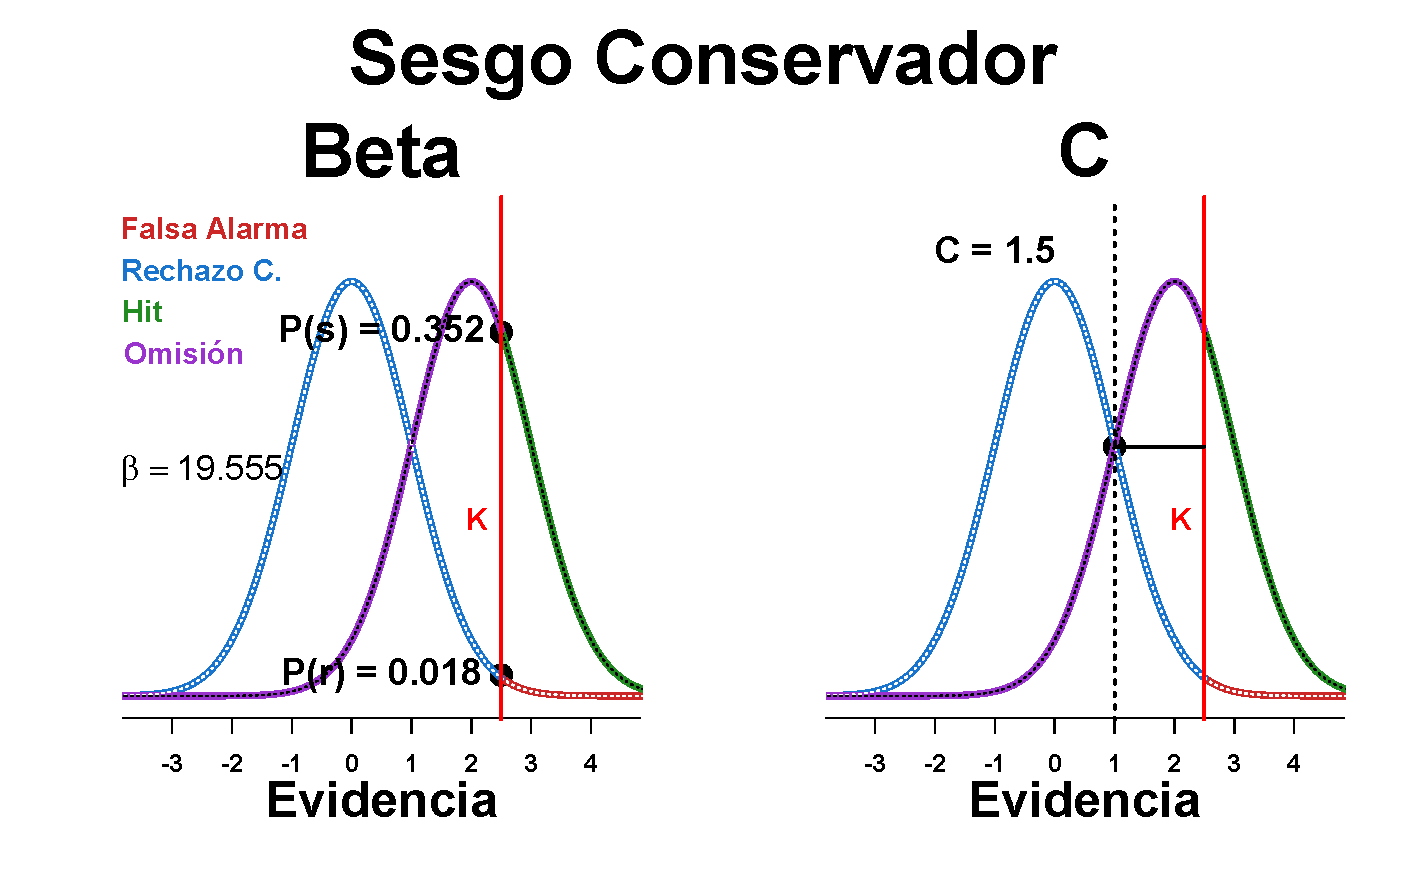
\includegraphics[width=0.8\textwidth]{Figures/Graficador_Sesgo_ConservadorR}\\
%\decoRule
\caption[Estimación paramétrica: Sesgos $\beta$ y $c$]{Se ilustra el cómputo de los parámetros de sesgo $\beta$ (figuras izquierdas) y $C$ (derechas), en casos donde el sesgo del sistema es liberal (el criterio se ubica en niveles bajos de evidencia; en el panel superior) o conservador (el criterio se sitúa sobre niveles altos de evidencia; panel inferior).}
\label{fig:Graf_Sesgo}
\end{figure}
\end{itemize} 

En la Figura~\ref{fig:Graf_Sesgo} se ilustra cada uno de los parámetros de sesgo descritos ($\beta$ en los paneles izquierdos y $C$ en los derechos), presentando en cada caso un ejemplo con sesgo liberal (en el panel superior) y con sesgo conservador (panel inferior). La diferencia entre ambos tipos de sesgos se desarrolla a continuación:\\

\begin{itemize}
\item \textsl{Sesgo liberal}. Implica una tendencia hacia la emisión de respuestas afirmativas aún con niveles bajos de evidencia, pues el criterio se encuentra orientado a la izquierda del eje de evidencia, (ver el panel superior de la Figura~\ref{fig:Graf_Sesgo}). Es decir: \\
\begin{center}
$C < 0$\\
ó\\
$0 < \beta < 1$\\
\end{center}

\item \textsl{Sesgo conservador}. Se presenta una tendencia hacia la emisión de respuestas negativas, pues el criterio se encuentra desplazado a la derecha del eje de evidencia, requiriendo una mayor cantidad de evidencia para la emisión de juicios afirmativos, (ver el panel inferior de la Figura~\ref{fig:Graf_Sesgo}). Es decir: \\
\begin{center}
$C > 0$\\
ó\\
$\beta > 1$\\
\end{center}

\item \textsl{Sesgo neutro}. No se favorece ninguna de las dos respuestas y la probabilidad de cometer cualquier acierto o cualquier error es la misma; el criterio se encuentra en $\frac{d'}{2}$. Es decir: \\
\begin{center}
$C = 0$\\
ó\\
$\beta = 1$\\
\end{center}
\end{itemize}

Para una exposición más detallada e interactiva de los parámetros descritos hasta ahora, se pueden consultar los graficadores y Apps en línea desarrollados por la autora de la presente tesis y otros colaboradores del Lab 25, como parte de un proyecto PAPIME (\citeyear{PAPIME}). Estos materiales se encuentran disponibles en \href{http://www.bouzaslab25.com/LabVirtual25/}{bouzaslab25.com/LabVirtual25}, un sitio web diseñado por la autora de esta tesis para los estudiantes de los cursos impartidos por el Dr. Arturo Bouzas.\\
%----------------------------------------------------------------

\subsection{Curvas ROC}

Además de permitir la descripción e interpretación del desempeño observado en tareas de detección a partir de la estimación de los parámetros descritos, los datos obtenidos en sesiones experimentales pueden ser utilizados para una evaluación más completa de la precisión con que el sistema podría responder a la misma tarea usando distintos criterio de elección. Las curvas ROC (identificadas así por su nombre en inglés: Receiver-Operating Characteristic Curve) describen la relación entre las tasas de Hits y Falsas Alarmas a obtener en tareas de detección con un valor partiular de $d'$, por cada localización posible del criterio sobre el eje de evidencia (McNicol \citeyear{McNicol2}; Egan, Schulman y Greenberg, \citeyear{Egan1959}; Swets, \citeyear{Swets1973}).\\

\begin{figure}[h]
\centering
%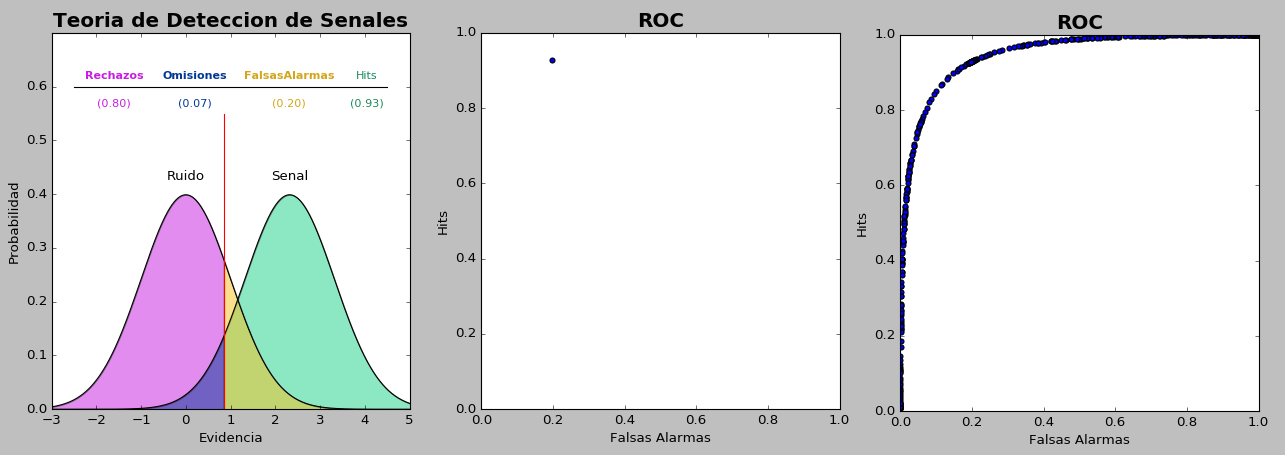
\includegraphics[width=0.90\textwidth]{Figures/Graficador_ROC12}\\
%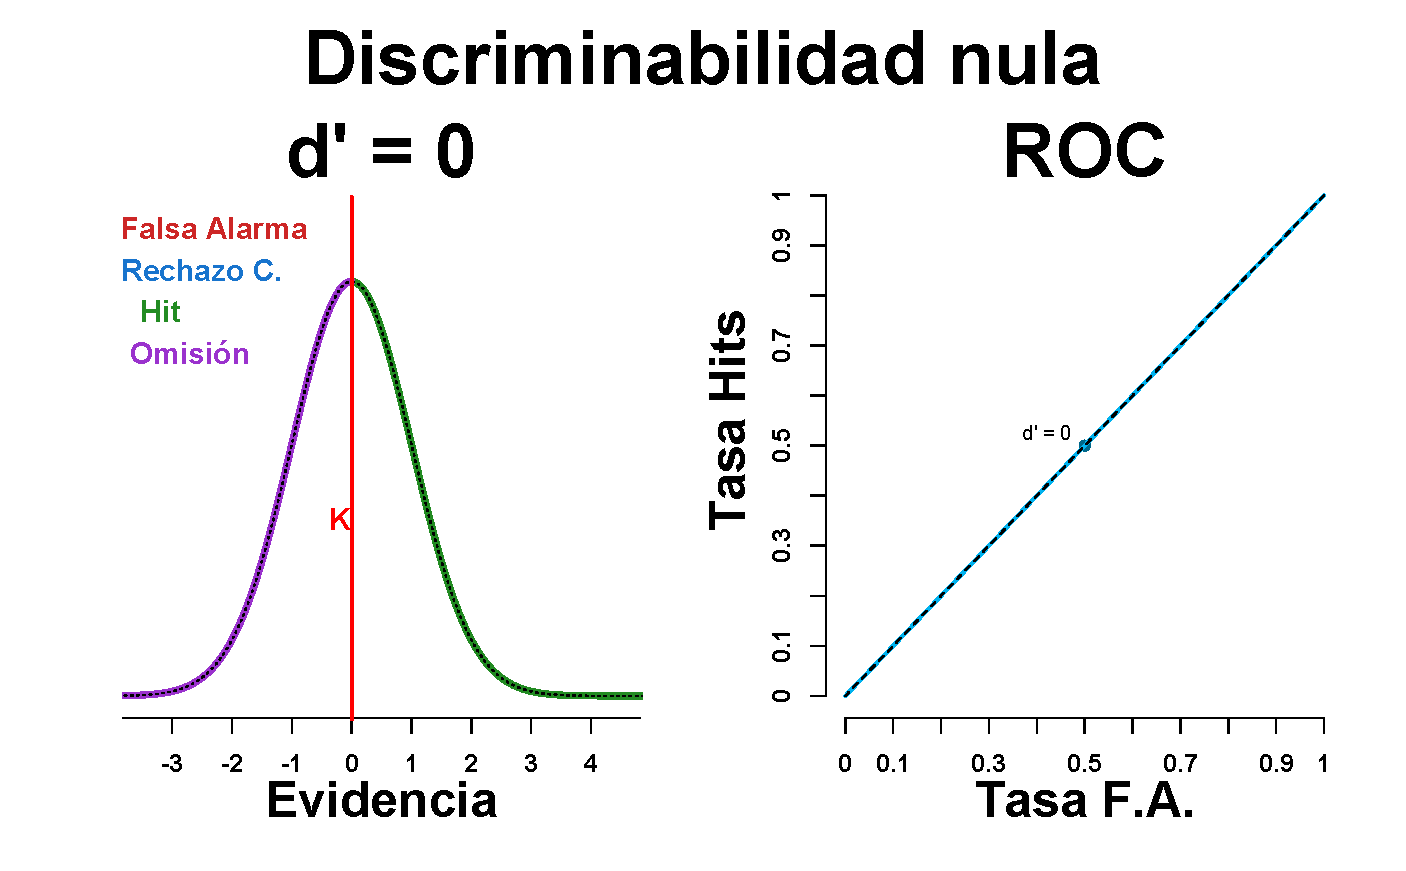
\includegraphics[width=0.9\textwidth]{Figures/ROC_1}\\
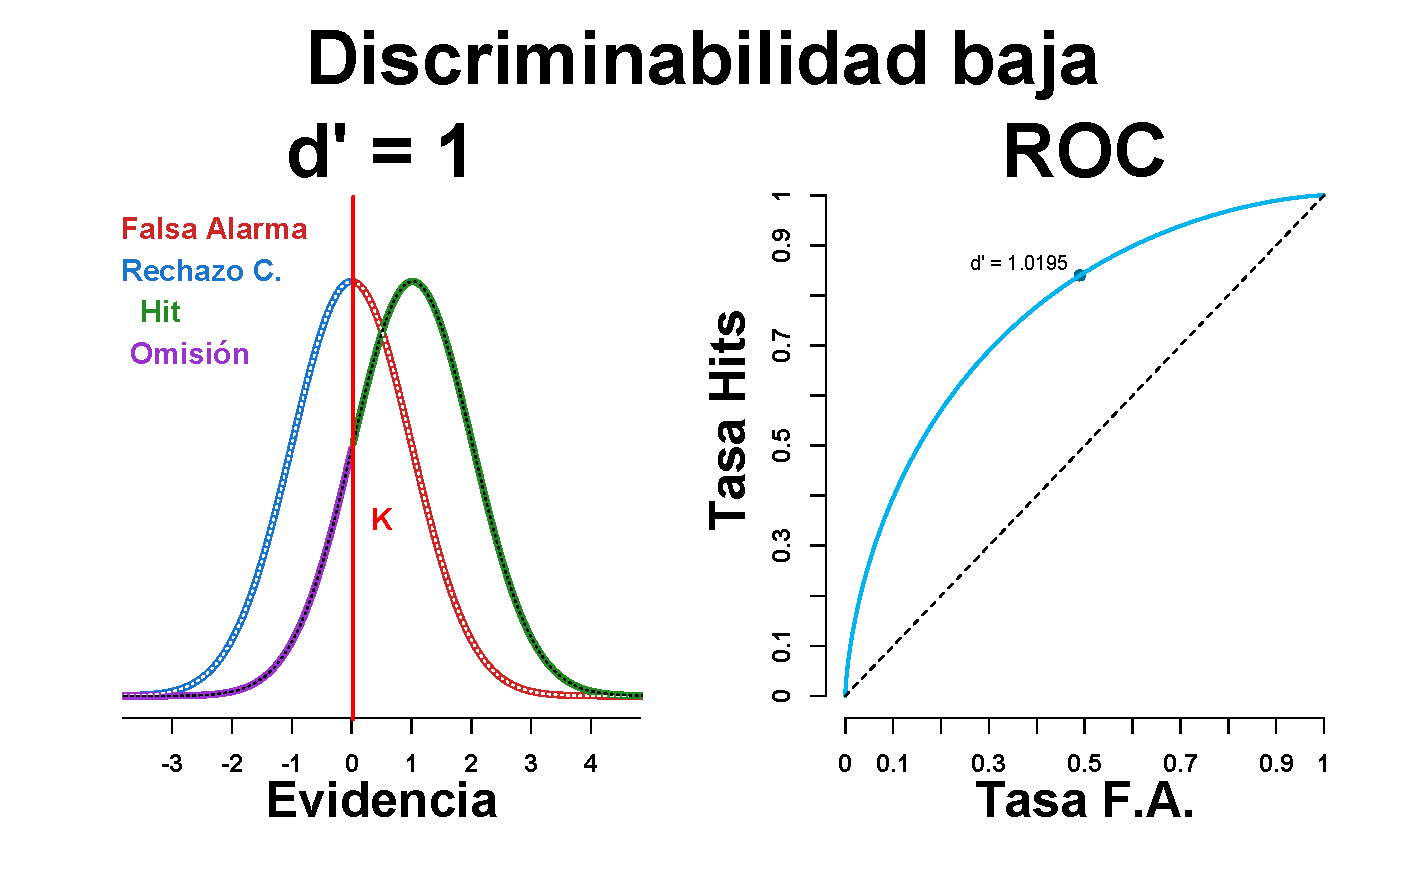
\includegraphics[width=0.75\textwidth]{Figures/ROC_2} \\
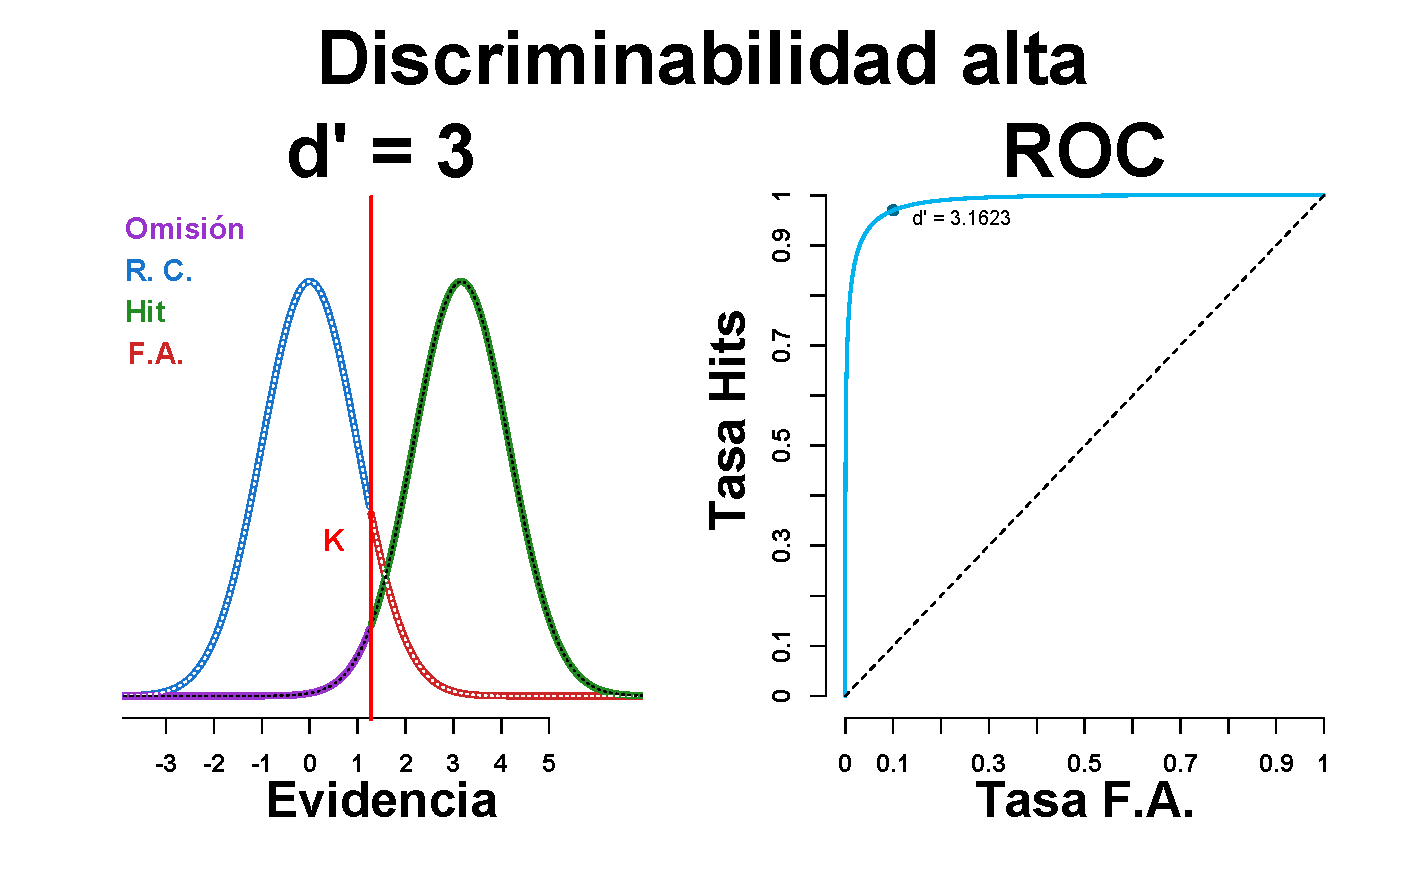
\includegraphics[width=0.75\textwidth]{Figures/ROC_3}\\
%\decoRule
\caption[Trazo de curvas ROC]{Ilustración del trazo de curvas ROC en dos escenarios con distinto nivel de $d'$. Los puntos marcados en las curvas ROC (figuras derecas) corresponden con la relación Tasa de Hits y Falsas Alarmas observadas dada la localización del criterio (figuras izquierdas). Las líneas contínuas azules en las curvas ROC representan los posibles pares a observar entre las tasas de Hits y Falsas Alarmas, dada la $d'$ computada, por cada valor que pueda ocupar el criterio.}
\label{fig:Graf_ROC}
\end{figure}

La Figura~\ref{fig:Graf_ROC} ilustra la construcción de curvas ROC a partir de las tasas de ejecución reportadas en tareas de detección. En las figuras izquierdas, se presenta un par de representaciones gráficas arbitrarias de tareas con distinto nivel de $d'$. Las figuras del lado derecho, señalan la intersección entre las tasas observadas de de Falsas Alarmas (eje x) y Hits (eje y) con un punto y, de acuerdo con el valor de $d'$ estimado, la curva que describe los posibles pares de Hits y Falsas Alarmas a observar con el uso de distintos criterios de elección. La idea central, es que por cada $d'$ se puede trazar una curva ROC que describa los resultados esperados para todos los valores posibles de $k$ (Tanner y Swets, \citeyear{Tanner1954}; Swets y cols.,  \citeyear{Swets1961}; Swets, \citeyear{Swets1973}; Stainslaw y Todorov, \citeyear{Stainslaw1999}).\\

%Bajo el supuesto de que lo único sobre lo que el sistema detector tiene injerencia es sobre el criterio de elección a usar para emitir sus juicios de detección, y que la discriminabilidad -al ser una cualidad inherente a los estímulos comprometidos en la tarea (ya sea por la variabilidad en su presentación o percepción)- es constante y ajena a este, \\

El área bajo la curva ROC (AUC, por sus siglas en ingles: Area Under the Curve) representa una forma precisa y completa de evaluar la sensibilidad del sistema detector ante la tarea estudiada (Centor y Schwartz, \citeyear{Centor1985}; Stainslaw y Todorov, \citeyear{Stainslaw1999}; McNicol, \citeyear{McNicol5}). Nótese que se habla de \textit{Sensibilidad} y no de \textit{Discriminabilidad} porque, aunque ambos conceptos refieren a qué tan fácil es para el sistema distinguir entre la señal y el ruido y se relacionan directamente con la distancia que existe entre sus distribuciones, la primera apela a la precisión con que el sistema detector puede responder a la tarea -utilizando distintas estrategias o reglas de elección- y la segunda, a una cualidad inherente a los estímulos (Swets, \citeyear{Swets1973}).\\

Como se mencionó anteriormente, en general se sabe que mientras más grande sea $d'$, existe una menor incertidumbre en la tarea de detección evaluada. Sin embargo, es complicado interpretar dicho valor en términos de qué tan \textit{buena} es la discriminabilidad. Es decir, parece poco claro qué tanto tendría que alejarse $d'$ de $0$ para afirmar que la Señal es discriminable del Ruido. Para ello, el cálculo del AUC proporciona información valiosa para la evaluación de la precisión con que el sistema puede responder a la tarea evaluada (Stainslaw y Todorov, \citeyear{Stainslaw1999}).\\ 

Cuando los estímulos con Señal son indistinguibles de los estímulos con Ruido ($d' = 0$), la curva ROC resultante se ve como una función de identidad. Esto implica que al emitir un juicio de detección afirmativo, existe la misma probabilidad de que este resulte en un Hit o una Falsa Alarma, con un AUC de 0.5 (la mitad del área total cae por debajo de la curva). Es decir, que mientras mayor sea el valor de $d'$, la curva ROC resultante se alejará más de la función identidad y su AUC será cada vez más cercano a 1.0. En general, el AUC puede tomar valores entre 0.5 -un sistema que no distingue en lo absoluto entre la Señal y el Ruido- y 1.0 -distinción perfecta entre los mismos- (Swets, \citeyear{Swets1973}; Stainslaw y Todorov, \citeyear{Stainslaw1999}; McNicol, \citeyear{McNicol5}).\\

Las curvas ROC pueden ser trazadas -en teoría- a partir de un solo conjunto de tasas de ejecución (Pollsvk y Norman, \citeyear{Pollack1964a}; Pollack, Norman y Galanter, \citeyear{Pollack1964b}; McNicol, \citeyear{McNicol2}) mediante algoritmos que asumen que el desempeño observado por parte del participante no puede \textit{mejorar} o \textit{empeorar} (dado que la discriminabilidad no depende de su conducta), y que se limitan a computar las tasa de ejecución que se esperaría observar en cada ubicación posible del criterio. Sin embargo, también pueden trazarse varios puntos para guiar el trazo de la curva ROC a partir de datos obtenidos en tareas donde experimentalmente se induzca el uso de distintos criterios de elección, obteniendo varios pares de tasas de Hits y Falsas Alarmas (Egan y cols., \citeyear{Egan1959}; Swets y cols., \citeyear{Swets1961}; Swets, \citeyear{Swets1986}). Los procedimientos mediante los cuales esto se lleva a cabo se discuten en la sección siguiente.\\

Al contar con datos obtenidos experimentalmente sobre el uso de distintos criterios de elección para responder a una misma tarea de detección, se puede trazar un tipo especial de curva ROC que permite explorar las características de las distribuciones de ruido y señal subyacentes. Para ello, en vez de graficar la relación entre las tasas observadas de Falsas Alarmas y Hits, éstas se transforman en puntajes Z para obtener lo que se conoce como una curva \textbf{z-ROC} que permite evaluar tres grandes factores (Ratcliff y cols., \citeyear{Ratcliff1992}):\\♠

\begin{itemize}
\item Si la curva z-ROC trazada es una línea recta, se acepta el supuesto de que las distribuciones de Ruido y Señal son normales.\\
\item La pendiente de la curva z-ROC permite conocer la razón entre las desviaciones estándar de las distribuciones de Ruido y Señal, evaluando así el supuesto de las varianzas iguales.\\
\item El intercepto de la curva z-ROC proporciona información sobre la distancia entre las distribuciones (un aproximado de $d'$).\\
\end{itemize}


%----------------------------------------------------------------

\subsection{Tareas de detección}

Para la interpretación y evaluación de tareas de detección, existen tres grandes protocolos empleados para obtener datos susceptibles de ser analizados bajo el marco de la SDT (McNicol, \citeyear{McNicol2}; Stainslaw y Todorov, \citeyear{Stainslaw1999}):\\

\begin{itemize}
\item \underline{Tareas de detección binaria}\\

La forma más sencilla y estándar de presentar una tarea de detección es con un procedimiento que únicamente solicite a los participantes la emisión de juicios binarios de detección (\textit{'Sí, la señal está'} o \textit{'No, no está'}). Dicho protocolo se identifica en la literatura con el nombre de \textbf{tareas de detección binaria} o \textbf{tareas Sí/No} (McNicol, \citeyear{McNicol2}).\\

Las tareas Sí/No realizadas en el laboratorio consisten en la presentación aleatoria de una serie de ensayos (N) compuesta por ensayos que contienen la señal (S) y ensayos con sólo ruido (R). En cada ensayo, la única respuesta que los participantes deben registrar es si la señal estuvo presente o no.\\

Típicamente, la cantidad de ensayos S y R presentados durante la tarea es la misma. Esto es recomendable por dos grandes razones: 1) Garantiza que las cuatro tasas de ejecución observadas sean igual de representativas del desempeño del participante, quien habría tenido el mismo número de oportunidades de cometer cada tipo de acierto y error, y 2) Evita que los participantes desarrollen un sesgo a favor de una respuesta particular dependiendo cuál sea el tipo de ensayo que más se le presente (Nevin, \citeyear{Nevin1969}; Wickens, \citeyear{Wickens1}).\\

Por cada tarea Sí/No conducida, se obtiene un conjunto de tasas de ejecución que permiten trazar uno solo de los puntos que componen la curva ROC que describe la sensibilidad del sistema evaluado. Así que, para obtener más datos con los cuales trazar la curva (más conjuntos de tasas de ejecución), tendría que correrse la misma tarea en repetidas ocasiones, con los mismos estímulos y en los mismos participantes, pero incitando el uso de distintos criterios de elección en cada ocasión. Esto se puede hacer de manera explícita (solicitándole al participante que sea más o menos estricto en la emisión de sus respuestas), o implícita (por ejemplo, presentando la tarea con distintas matrices de pago que lleven al participante a evitar un cierto tipo de error, o a buscar cierto tipo de acierto) (Wickens, \citeyear{Wickens1}; McNicol \citeyear{McNicol2}.\\

Un problema evidente con el trazo de curvas ROC a partir de los datos obtenidos en tareas de detección binarias repetidas es que requiere un número considerable de repeticiones, todas compuestas por el mismo número de ensayos. Exponer a un mismo participante a la misma tarea varias veces trae consigo el riesgo de que su desempeño se vea afectado por la fatiga o el aprendizaje. Si este fuera el caso, los datos obtenidos no sólo serían reflejo de cambios en el criterio usado para responder a la tarea, sino que incluso podría haberse alterado la discriminabilidad de la misma (el aprendizaje puede hacer que los participantes se vuelvan mejores distinguiendo entre la Señal y el Ruido, y la fatiga, tener el efecto opuesto). Esto representa un problema porque entonces, la curva ROC trazada no representaría la sensibilidad del sistema evaluado ante \textit{una misma} tarea, pues se estaría violando el supuesto fundamental de que la discriminabilidad es constante (McNicol, \citeyear{McNicol2}).\\

\item \underline{Tareas con Escala de Confianza}\\

Una segundo protocolo para la presentación de tareas de detección -que puede entenderse como una extensión de las tareas Sí/No- es solicitando a los participantes que valoren y asignen un puntaje a la certeza que tienen sobre la pertenencia de cada estímulo evaluado a las categorías Señal o Ruido, de acuerdo con una \textbf{Escala de Confianza}.\\

En términos del procedimiento, las tareas de detección binarias y con Escala de Confianza son idénticas: se muestra a los participantes una serie de ensayos (N) dentro de la cual se presentan de manera aleatoria ensayos con la señal (S) y ensayos con sólo Ruido (R), solicitándoles que registren una respuesta al término de cada ensayo. La diferencia entre ambos protocolos consiste en el tipo de respuesta solicitada y, en consecuencia, la cantidad de información que se obtiene sobre la sensibilidad del sistema. En las tareas Sí/No los participantes emiten una de dos posibles respuestas mutuamente excluyentes; en tareas con Escala de Confianza, se asigna un puntaje dentro de una Escala con cierta cantidad de opciones de respuesta (Stainslaw y Todorov, \citeyear{Stainslaw1999}).\\

Existen varias formas en que puede presentarse la Escala de Confianza (McNicol, \citeyear{McNicol2}). Por ejemplo, una de ellas podría ser solicitando que se responda de acuerdo a la confianza que se tendría en asignar cada estímulo evaluado a la categoria Señal (donde los valores más altos se asignarían a los estímulos que se encuentren más hacia la derecha en el eje de evidencia y los valores bajos, a los estímulos con Ruido, a la izquierda). Por otro lado, una segunda forma sería distinguiendo entre la certeza que se tiene sobre la pertenencia de cada estímulo evaluado al conjunto de las señales o el ruido, (los valores más altos indicarían confianza en que se trate de una Señal y los valores más bajos, de que se trate de Ruido). Ambas formas de presentar la Escala proporcionan -en teoría- la misma información, tal y como se sugiere en el panel superior de la Figura~\ref{fig:Conf_Rat}. En general, la elección de una u otra depende del experimentador.\\

\begin{figure}[h]
\centering
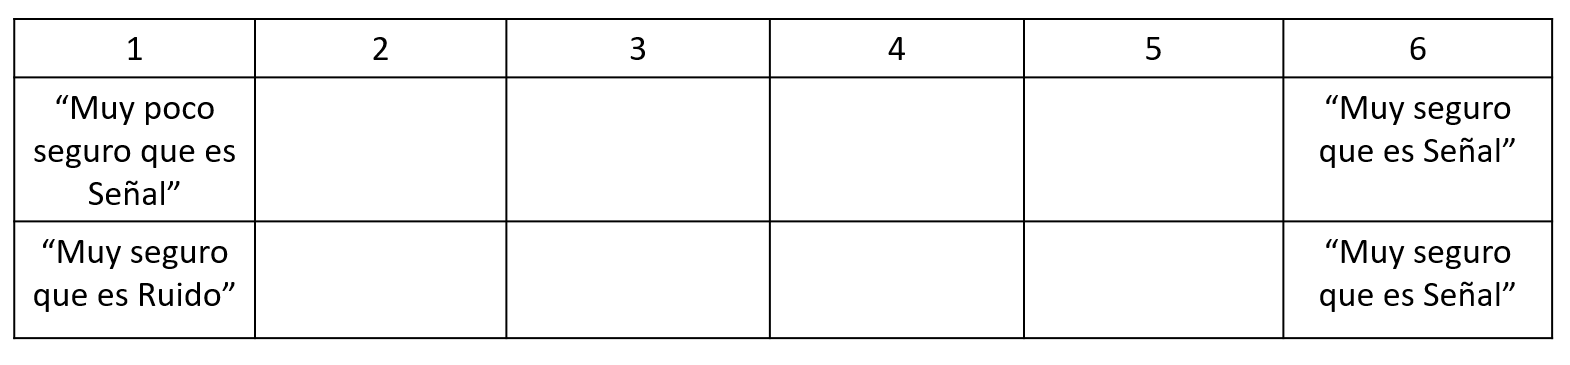
\includegraphics[width=0.9\textwidth]{Figures/Puntajes_Criterios}\\
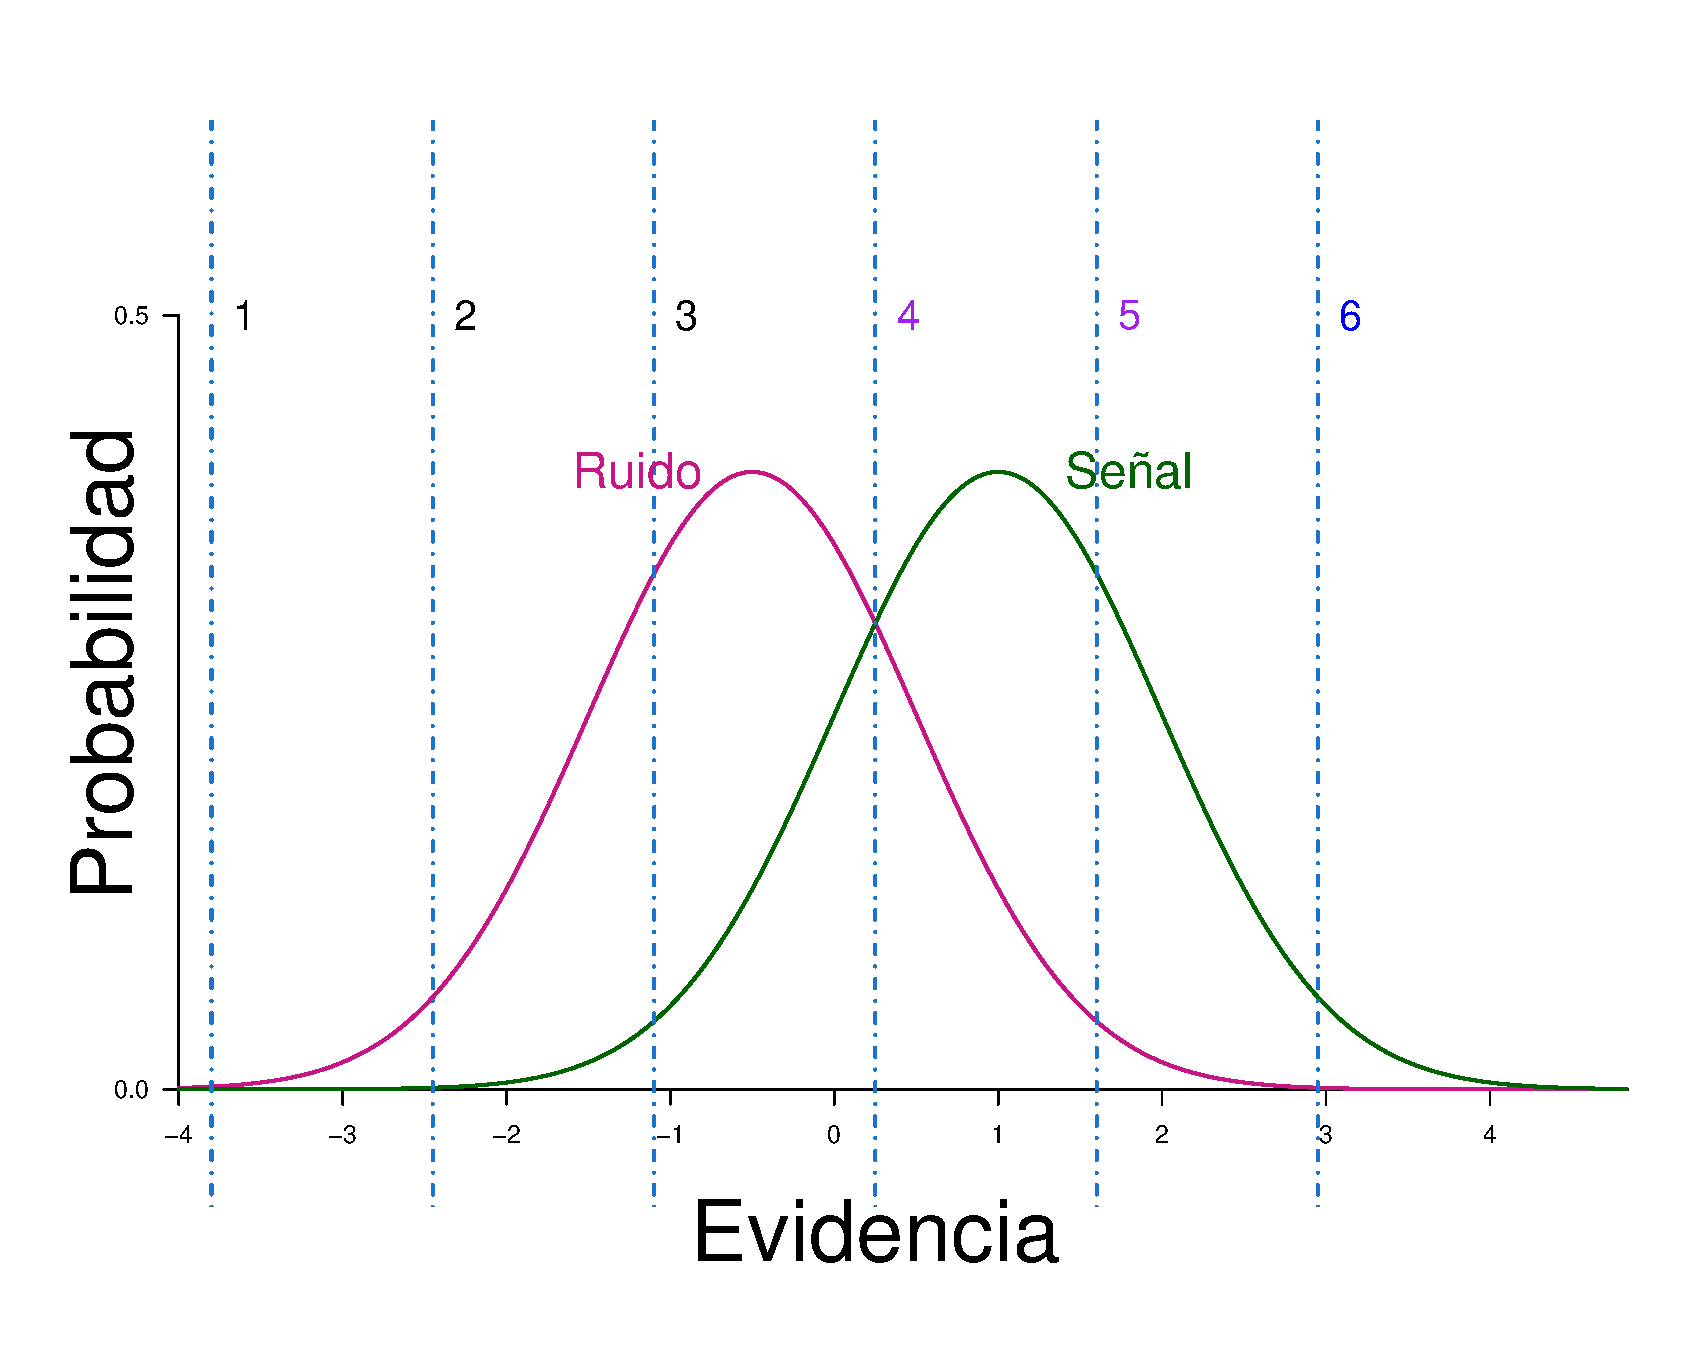
\includegraphics[width=0.70\textwidth]{Figures/ConfidenceRating}\\
%\decoRule
\caption[Tareas de detección con Escala de Confianza y su interpretación]{Representación gráfica de la interpretación de las tareas de detección con Escala de Confianza bajo el marco de la SDT. En la parte superior se presenta una Escala de Confianza de seis elementos con dos posibles sentidos: unidireccional (el puntaje refleja la confianza en una sola respuesta) o bidireccional (el puntaje distingue entre la confianza en cada respuesta). La gráfica inferior ilustra la idea de que para decidir cuándo emitir cada puntaje, el sistema fija múltiples sub-criterios sobre el eje de evidencia.}
\label{fig:Conf_Rat}
\end{figure}

Los puntajes de confianza registrados son interpretados asumiendo que los participantes fijan un criterio por cada opción de respuesta incluida en la Escala de Confianza. De esta forma, el puntaje emitido en cada ensayo está determinado por el último criterio de elección rebasado por la evidencia evaluada (McNicol, \citeyear{McNicol2}). La Figura~\ref{fig:Conf_Rat} ilustra esta idea: en la parte superior se presenta una Escala de Confianza de 6 elementos (se ejemplifican las dos formas -previamente expuestas- en que puede ser presentada), y en la parte inferior, la representación gráfica de su interpretación bajo el modelo de detección de señales.\\

El protocolo de Escala de Confianza permite recabar información sobre el uso de múltiples criterios de elección -tantos como opciones de respuesta se incluyan en la Escala- en una tarea de detección particular con un solo experimento, manteniendo constante la discriminabilidad. Por ello, el uso de Escala de Confianzas con $n$ opciones de respuesta, representa una forma sencilla y directa de obtener datos suficientes para trazar $n - 1$ puntos en una curva ROC y poder evaluar con mayor certidumbre la sensibilidad del sistema (Stainslaw y Todorov, \citeyear{Stainslaw1999}; McNicol, \citeyear{McNicol2, McNicol5}).\\ 

Idealmente, se espera que el participante utilice todas las opciones de respuesta incluídas en la Escala de Confianza. Esto se puede conseguir de manera explícita o implícita, solicitando a los participantes que lo hagan así, o bien, modificando el número de puntajes incluídos en la Escala. En general, se recomienda que la Escala esté compuesta por un número par de opciones de respuestas que oscile entre 4 y 10 (McNicol, \citeyear{McNicol2, McNicol5}). Esto con el fin de evitar que los participantes elijan la opción intermedia cuando se sientan inseguros sobre su respuesta.\\

\pagebreak
\item \underline{Tarea de Elección forzada}\\

Existe un tercer protocolo bajo el cual se presentan las tareas de detección, identificado como \textbf{tareas de Elección forzada entre $m$ alternativas}, donde se presentan simultáneamente $m - 1$ estímulos que contienen sólo ruido y $1$ con señal, y la tarea del participante consiste en identificar la Señal dentro del conjunto de estímulos que se le presentan (Stainslaw y Todorov, \citeyear{Stainslaw1999}). En general, se asume que cada estímulo presentado contiene cierto valor de evidencia -cierta ubicación en el eje sobre el cual se despliegan las distribuciones- que el participante compara para elegir aquel que tenga un valor mayor -de acuerdo con el supuesto que establece que, en general, los valores de la distribución Señal caen por encima del Ruido- (McNicol, \citeyear{McNicol2}).\\

%Dada la relación que representan, el área bajo la curva ROC trazada con un protocolo de preguntas binarias o con Escala de Confianza puede interpretarse como la proporción de veces que el participante cuyo desempeño se describe, podría identificar correctamente la Señal, si esta fuera presentada simultáneamente junto con el Ruido. A su vez, la proporción de respuestas correctas obtenidas a lo largo de una tarea de Elección forzada proporciona una medida de la sensibilidad del sistema, independiente del sesgo del sistema. Dicha medida -al igual que el AUC-, tendría que variar entre el azar ($\frac{1}{m}$) y el desempeño perfecto ($1.0$), \citep{Stainslaw1999}.\\
\end{itemize}


















\section{Teoría de Detección de Señales en Memoria}

La Teoría de Detección de Señales ha sido ampliamente utilizada en distintas áreas de la Psicología Experimental tanto como marco de referencia para la descripción de diversas situaciones de detección, como herramienta para el análisis de datos obtenidos en dichas tareas. Una de estas áreas refiere al estudio de la Memoria, donde los supuestos y conceptos desarrollados en la SDT han sido aplicados para explicar el funcionamiento del aprendizaje humano, la retención, el olvido y el reconocimiento de estímulos (Murdock, \citeyear{Murdock1965}; Bernbach, \citeyear{Bernbach1967}; Lockhart y Murdock, \citeyear{Lockhart1970}; Banks, \citeyear{Banks1970}; White y Wixted, \citeyear{White1999}).\\

%Al estudiar las tareas presentadas en estudios de memoria como instancias de un problema de detección, los resultados obtenidos pueden clasificarse dentro de las mismas categorías presentadas anteriormente en la matriz de la Figura~\ref{fig:Mat_Output}), permitiendo así que las tasas de Hits y Falsas Alarmas registradassean uilizadas para trazar curvas ROC (Egan, \citeyear{Egan1958}; Zandt, \citeyear{VanZ2000}), con frecuencia identificadas como curvas MOC (por sus siglas en inglés \textit{Memory Operant Curve}), (Norman y Wickelgreen, \citeyear{Norman1965}; Kintsch y Carlson, \citeyear{KintschCarlson1967}).\\

La aplicación de la SDT al estudio de la memoria ha impactado en el desarrollo de este útlimo en términos de cuatro grandes ejes (Banks, \citeyear{Banks1970}), que son:\\

\begin{enumerate}
\item La noción de la \textit{Fuerza de Memoria}.\\

Aceptar la SDT como marco para describir el funcionamiento de los distintos mecanismos estudiados en Memoria implica asumir que la \textit{evidencia} con base en la cual se emiten las respuestas ensayo a ensayo son valores ($x$) dentro de un eje contínuo sobre el cual se despliegan las distribuciones de Ruido (los estímulos distractores) y Señal (estímulos definidos de acuerdo al procedimiento empleado). Los modelos de memoria que incorporan la SDT como base para el desarrollo de su marco explicativo, tienden a interpretar dicho valor $x$ como un reflejo de la \textit{fuerza de memoria}, o bien, un índice de qué tan \textit{relacionable} o \textit{familiar} resulta para el sistema cada estímulo evaluado (Ratcliff, Ching-FanSheu y Gronlund, \citeyear{Ratcliff1992}). Así pues, se interpreta el desempeño observado en los participantes como resultado de la interacción entre la \textit{fuerza de memoria} evaluada en cada ensayo y un proceso de decisión que determina si ésta es lo suficientemente grande para juzgar la pertenencia de cada estímulo a la categoría Señal.\\

%En términos de la exploración de este supuesto y sus implicaciones, resaltan los trabajos orientados a evaluar la naturaleza de dicha \textit{fuerza de memoria} (por ejemplo, si puede entenderse a partir de valores contínuos o discretos), y su interacción con los procesos propios de la Memoria (por ejemplo, el estudio, la retención y el olvido), (Bernbach, \citeyear{Bernbach1967}; Wickelgreen y Norman, \citeyear{Wickelgren1966}; Parks, \citeyear{Parks1966}).\\

\item La noción del Criterio de Elección como opuesta a los Umbrales de respuesta.\\

Una de las aportaciones más evidentes de la aplicación de los principios propuestos por la SDT al estudio de la Memoria es que permite entender los Falsos Positivos en términos de una confusión entre la fuerza de memoria producida por un estímulo distractor y la Señal (el área de sobrelape entre las distribuciones), y abandonar el supuesto de que cuando las señales a detectar están ausentes, los participantes responden a la tarea de manera aleatoria. Con ello, se abandona la noción originada en la Teoría del Umbral de que existe tal cosa como un \textit{umbral de memoria} que debe ser rebasado para que el sistema sea capaz de identificar la pertenencia de los estímulos a una u otra categoria (Murdock, \citeyear{Murdock1982}; Gillund y Shiffrin, \citeyear{Gillund1984}; Yonelinas, Dobbins, Szymanski Dhaliwal y King, \citeyear{Yonelinas1996}; Wixted, \citeyear{Wixted2007}). Con ello, tal y como ocurrió tras la incorporación de la SDT al estudio de la Percepción, los procesos de Memoria comienzan a ser concebidos como instancias de un proceso de decisión (Bernbach, \citeyear{Bernbach1967}).\\
 
\item La noción de que existen distribuciones subyacentes (y la definición de sus características).\\

Los datos obtenidos en experimentos de memoria donde se promueva el uso de diversos criterios de elección pueden utilizarse para construir curvas \textbf{MOC} (por sus siglas en inglés, Memory Operating Characteristic curve) que describan la precisión con que los participantes distinguen entre los estímulos con ruido y señal, (Kintsch, \citeyear{Kintsch1967}; Ratcliff y cols., \citeyear{Ratcliff1992}; Ratcliff, McKoon y Tindall, \citeyear{Ratcliff1994}). Así mismo, el trazo de curvas MOC a partir de las transformaciones a puntajes Z de las tasas de Hits y Falsas Alarmas registradas (lo que serían las curvas z-MOC), ha permitido explorar la naturaleza de las distribuciones subyacentes (Ratcliff y cols., \citeyear{Ratcliff1992}), los hallazgos e implicaciones de este tipo de análisis se desarrollan más adelante.\\
\end{enumerate} 

\subsection{Memoria de Reconocimiento}

%Por mucho tiempo, los modelos desarrollados en Memoria estuvieron muy limitados en términos del espectro de tareas y fenómenos de los que permitían dar cuenta. No fue hasta que comenzaron a surgir los \textit{modelos globales de memoria}, que incorporaron los principios básicos de la SDT, que fue posible explicar una gama más amplia de tareas y mecanismos dentro del área. Estos modelos se distinguen principalmente por los supuestos que hacen sobre el tipo de distribuciones que capturan la variabilidad contenida en los estímulos con ruido y señal, y la forma en que se define la fuerza de memoria en la interacción entre los distintos sistemas de memoria y los estímulos (Murdock, \citeyear{Murdock1982}; Gillund y Shiffrin, \citeyear{Gillund1984}; Eich, \citeyear{Eich1985}). Cada uno de estos modelos ha sido desarrollado para dar cuenta de un sub-set específico de tareas y fenómenos (recuerdo, juicios de frecuencia, olvido y retención, entre otros), encontrando un punto de convergencia en el estudio de la Memoria de Reconocimiento (Parks, \citeyear{Parks1966}; Ratcliff y cols., \citeyear{Ratcliff1992}).\\

Los modelos que incorporan la SDT para dar cuenta de la Memoria de Reconocimiento aparecen como una alternativa a los modelos clásicos que adoptaban la idea de \textit{umbrales de respuesta}. Un ejemplo representativo de este tipo de aproximación es la Teoría del Procesamiento Dual que plantea que existen dos procesos, mutuamente excluyentes, que determinan la emisión de juicios de reconocimiento (la recolección y el análisis de familiaridad), siendo que el proceso dominante se impone en función a qué tan familiar sea el estímulo evaluado respecto de cierto umbral (Yonelinas y cols., \citeyear{Yonelinas1996}; Wixted, \citeyear{Wixted2007}).\\

Aplicar la SDT al estudio de la memoria de reconocimiento implica entender las tareas de reconocimiento como una instancia de tareas de detección, donde los participantes tienen que identificar dentro de una lista de elementos, cuáles ya se le habían mostrado en una fase previa de estudio (los \textit{estímulos viejos}: las señales) y cuáles no (los \textit{estímulos nuevos}: el ruido), (Bernbach, \citeyear{Bernbach1967}; Kintsch, \citeyear{Kintsch1967}). Bajo este esquema, la 'fuerza de memoria' refleja el grado en que un estímulo cualquiera es percibido como 'familiar' para el sistema y su comparación con el criterio de elección es lo que determina la respuesta dada por el mismo (\textit{'Sí, es un elemento antes visto'} o \textit{'No'}).\\ 

\begin{figure}[h]
\centering
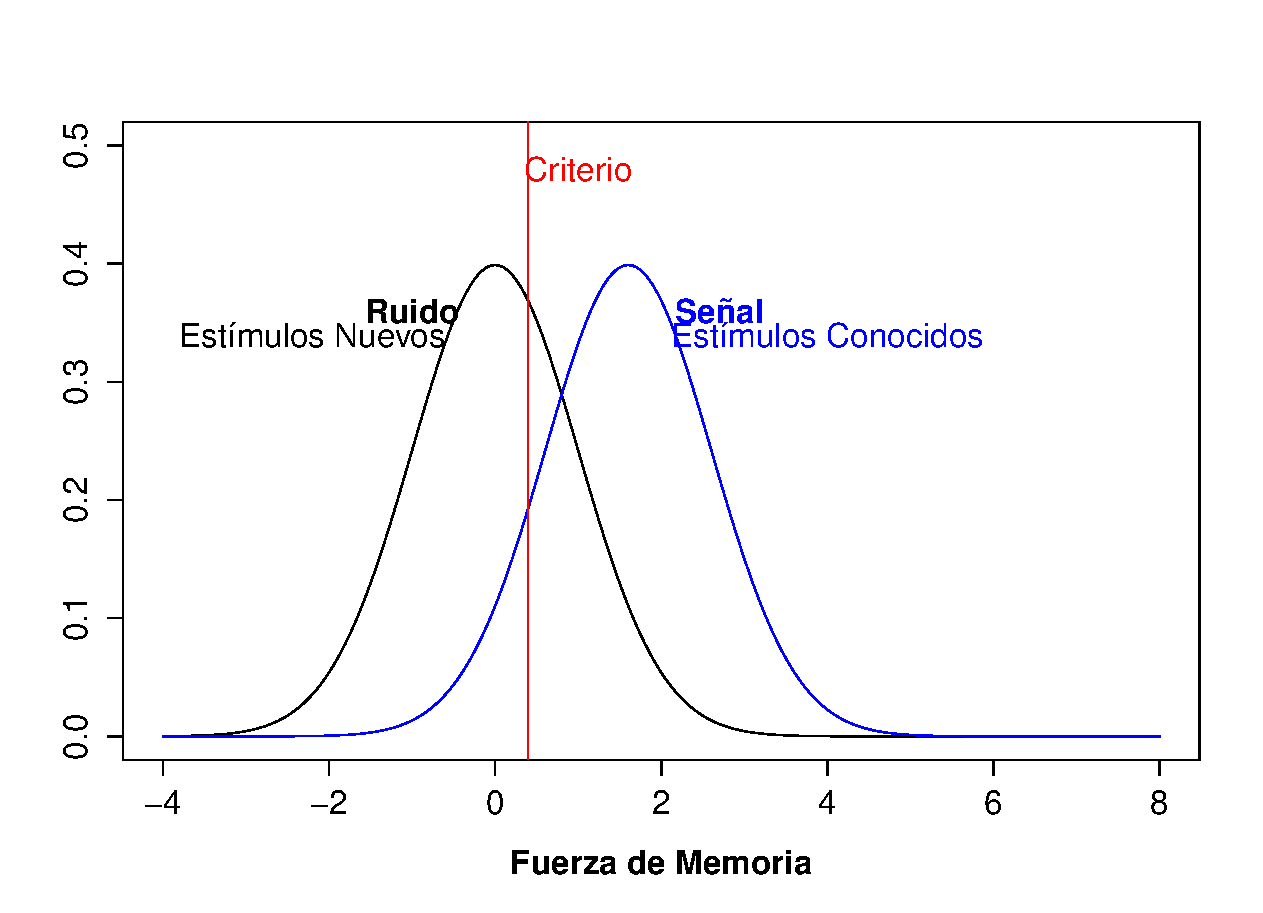
\includegraphics[width=0.8\textwidth]{Figures/RM_SDT_1} 
\caption[SDT aplicada a tareas de memoria de reconocimiento]{Representación gráfica de la aplicación de la SDT al estudio de tareas de memoria de reconocimiento}
\label{fig:RM_SDT_1}
\end{figure}

La Figura~\ref{fig:RM_SDT_1} ilustra la forma en que los supuestos y conceptos básicos de la SDT se aplican al contexto de la memoria de reconocimiento: Los estímulos ya conocidos (referidos como \textit{estímulos viejos}) constituyen la Señal y el Ruido lo componen estímulos nuevos que pueden ser confundidos con los viejos. El \textit{eje de evidencia} a lo largo del cual se despliegan las distribuciones se convierte en un \textit{eje de familiaridad}, que contiene distintos valores de 'fuerza de memoria' (siendo que los estímulos viejos tienen valores más altos de 'familiaridad' que los estímulos nuevos). Por último, se incorpora la idea de que la emisión de juicios de reconocimiento depende de la comparación entre la 'familiaridad' evaluada en cada ensayo y un criterio de elección fijado por el participante.\\

Las tareas de reconocimiento conducidas en el laboratorio suelen componerse de dos fases (Ratcliff y cols., \citeyear{Ratcliff1992}). En la primera (\textit{la fase de estudio}) se presenta a los participantes una serie de elementos para que los estudien de manera intencional (solcitándoles explícitamente que las estudien para su reconocimiento posterior) o incidental (planteándoles alguna tarea distractora que los obligue a interactuar con ellos) (Noldy, Stelmack y Campbell, \citeyear{Noldy1990}). En la segunda fase (la \textit{fase experimental} o \textit{de reconocimiento}) se presentan los mismos elementos incluidos en la primera fase, más una cantidad igual de elementos nunca antes presentados. La tarea de los participantes consiste en identificar cuáles de los elementos que se le presentan en la segunda fase son \textit{estímulos viejos}, previamente incluídos en la fase de estudio.\\

De acuerdo con las curvas z-ROC que se obtienen a partir de los datos obtenidos en estudios con tareas de reconocimiento, se ha concluído que el modelo basado en SDT que mejor describe la ejecución de los participantes es uno donde las distribuciones de Ruido y Señal son normales, siendo menor la varianza en la distribución de Ruido que en la distribución de Señal (Ratcliff y cols., \citeyear{ Ratcliff1992}, {Ratcliff1994}). Tal y como se ilustra en la Figura~\ref{fig:RM_SDT_2}, consistentemente se reporta que la razón entre las desviaciones estándar de la distribución de Ruido y Señal tiene valores cercanos a 0.8 (Wixted, \citeyear{Wixted2007}).\\

\begin{figure}[h]
\centering
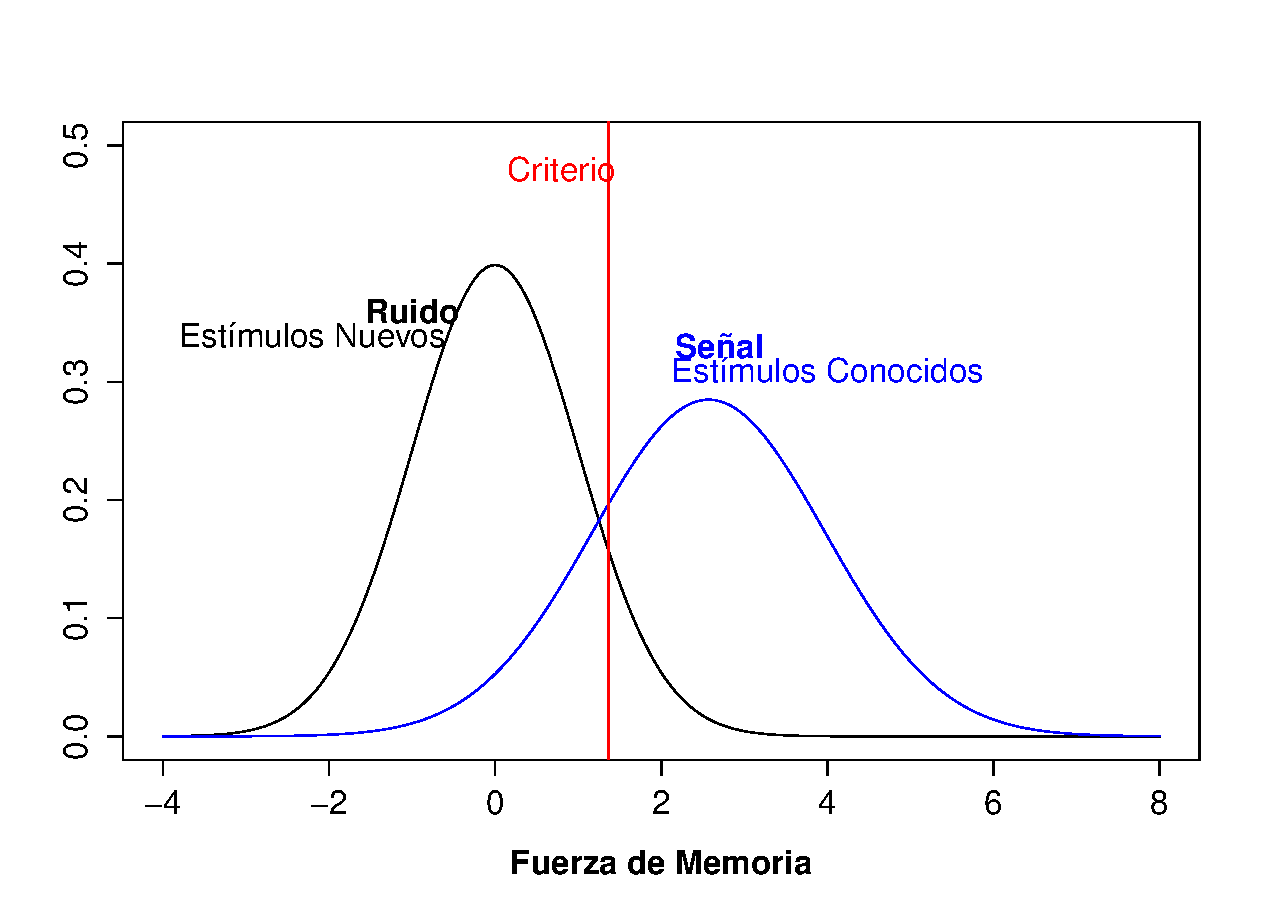
\includegraphics[width=0.80\textwidth]{Figures/RM_SDT_2} 
\caption[SDT en memoria de reconocimiento (varianzas desiguales)]{Representación gráfica del modelo de varianzas desiguales reportado en memoria de reconocimiento, al estudiarse bajo el marco de la SDT.}
\label{fig:RM_SDT_2}
\end{figure}








\section{El Efecto Espejo}

El 'Efecto Espejo' hace referencia a la interpretación de ciertos patrones de respuestas reportados consistentemente en estudios de memoria de reconocimiento donde el desempeño de los participantes es comparado a través de dos clases de estímulos que difieren en la precisión con que se sabe que sus elementos suelen reconocerse, bajo el marco de la SDT. Típicamente, dichas clases son referidas en la literatura como Clase A, con estímulos fácilmente reconocibles, y Clase B, con estímulos que se reconocen con mayor dificultad, (siendo que $d'(A) > d'(B)$), (Glanzer y Adams, \citeyear{Glanzer1990}). En estos estudios, se ha encontrado evidencia sólida de que las diferencias en la discriminabilidad de los estímulos Nuevos y Viejos de las clases A y B se mantienen en dos sentidos: en la identificacíón de los estímulos viejos como \textit{Viejos} (más Hits en A que en B) y en la identificación de los estímulos nuevos como \textit{Nuevos} (menos Falsas Alarmas en A que en B). Es decir, se ha encontrado evidencia que sugiere que las diferencias en $d'$ no sólo impactan en el número de Hits cometidos, sino también en la propoción observada de Falsas Alarmas (Glanzer, Adams, Iverson y Kim, \citeyear{Glanzer1993}).\\

Al interpretar las tasas de Hits y Falsas Alarmas registradas por cada clase bajo el marco de la SDT, se sugiere que existen cuatro distribuciones que subyacen a la tarea: dos distribuciones para los estímulos señal de cada clase y dos distribuciones de ruido. Y de acuerdo con los patrones de respuesta registrados, el orden en que se presentan las distribuciones de estímulos Viejos A y B es el inverso (el \textit{reflejo}) del orden en que se presentan las distribuciones de estímulos Nuevos respectivas (Glanzer y Adams, \citeyear{Glanzer1990}; DeCarlo, \citeyear{DeCarlo2007}). La representación gráfica de este orden (Nuevos(A), Nuevos(B), Viejos(B) y Viejos(A)), se presenta en la Figura~\ref{fig:Ejem_EfectoEspejo} e ilustra la razón por la cual se ha identificado dicho fenómeno con el nombre de Efecto Espejo.\\

\begin{figure}[h]
\centering
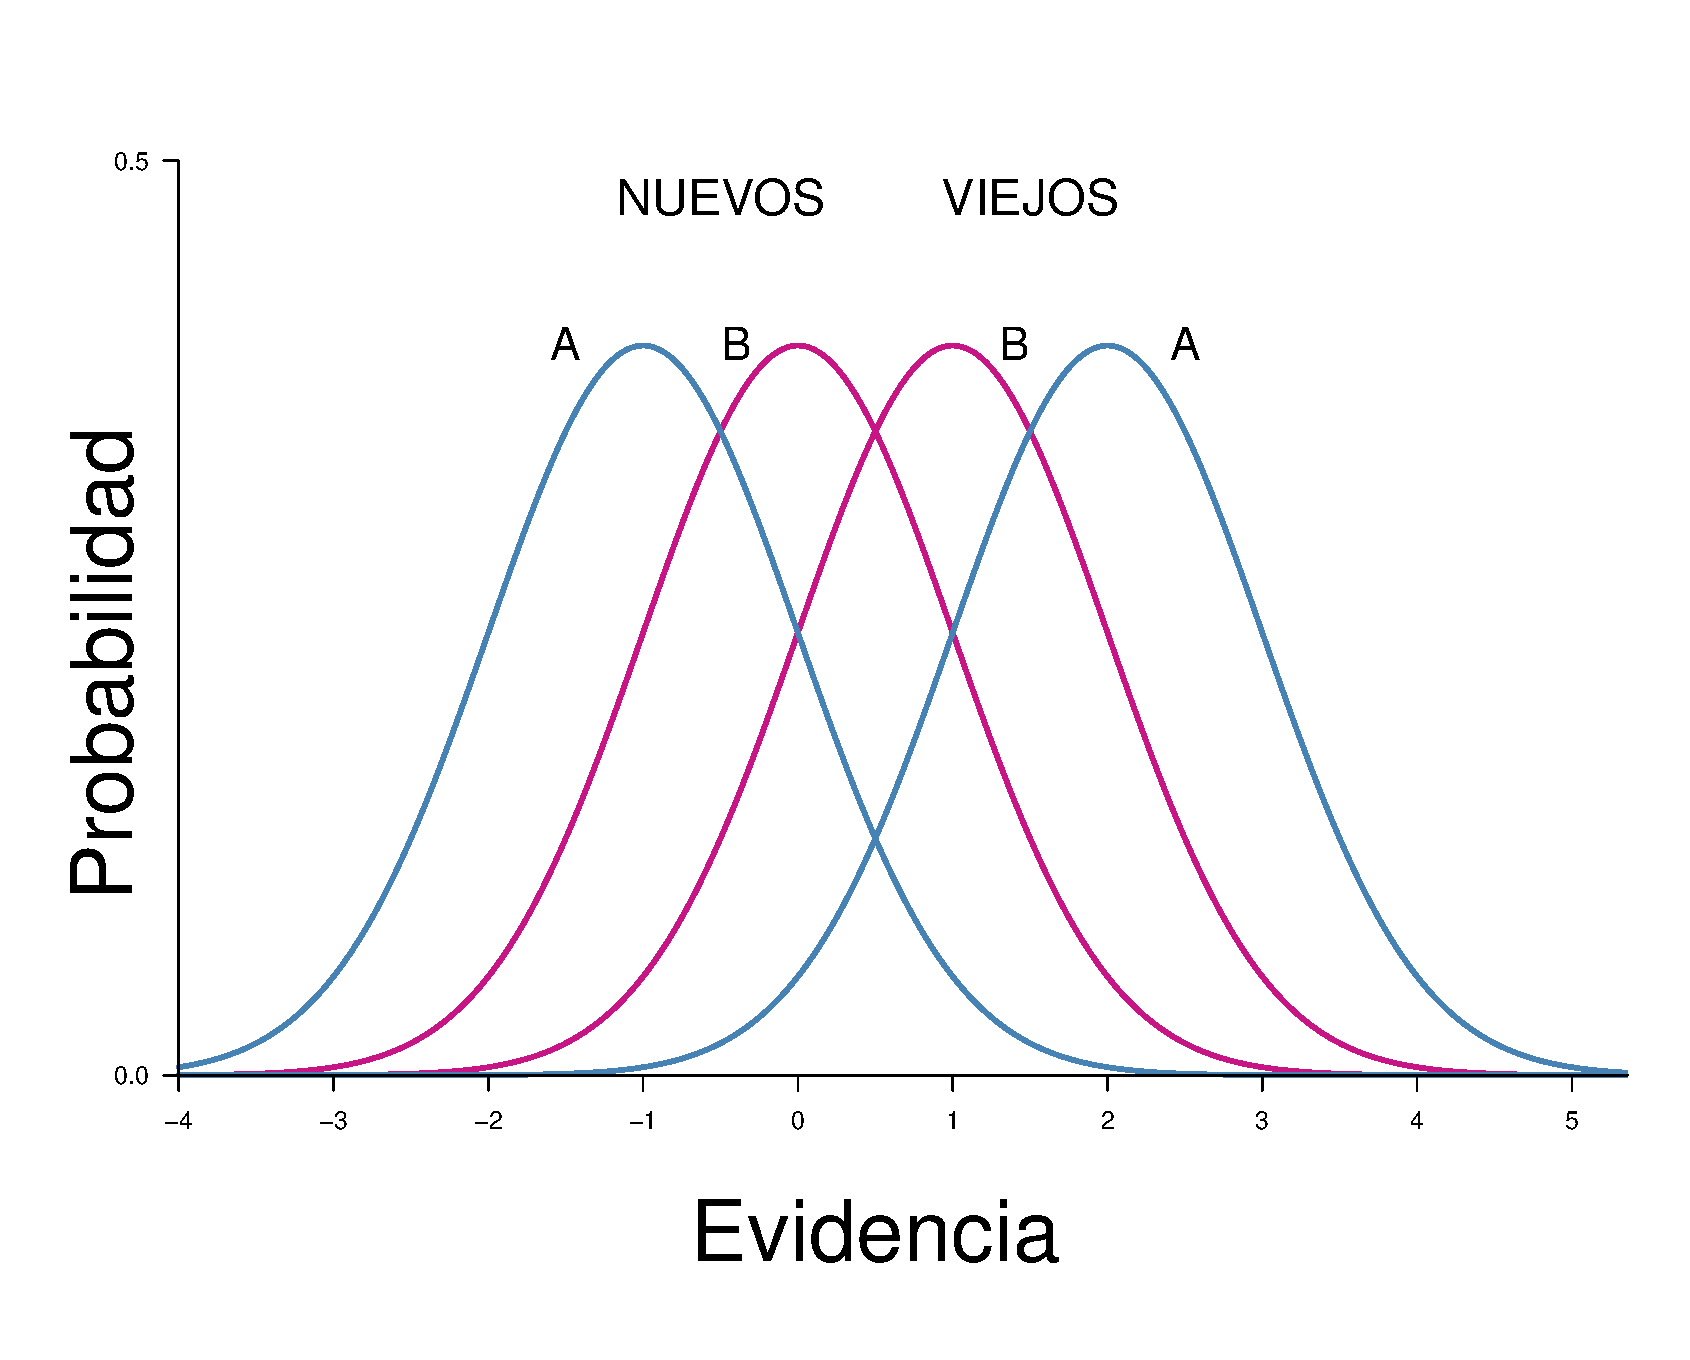
\includegraphics[width=0.7\textwidth]{Figures/EfectoEspejo}
%\decoRule
\caption[Efecto Espejo: Las distribuciones de ruido y señal A y B se reflejan entre sí]{Representación gráfica de la ubicación de las distribuciones de ruido y señal (de las clases A y B) sobre el eje de evidencia, de acuerdo con los patrones de respuesta encontrados en tareas memoria de reconocimiento, identificados como Efecto Espejo.}
\label{fig:Ejem_EfectoEspejo}
\end{figure}

La evidencia a favor del Efecto Espejo en experimentos de memoria de reconocimiento se reporta a lo largo de una amplia variedad de clases de estímulos y protocolos de tareas de detección (Preguntas Sí/No; Escala de Confianza y Elección Forzada de dos alternativas), (Glanzer y Adams, \citeyear{Glanzer1990}), siempre y cuando se cumplan las siguientes condiciones:\\

\begin{itemize}
\item Existen al menos dos clases de estímulos A y B entre las cuales se compara el desempeño de los participantes. A y B difieren en su nivel de discriminabilidad: la clase A se caracteriza porque sus elementos se reconocen con mayor facilidad que los estímulos contenidos en B.\\

\item Los estímulos que componen las clases A y B se presentan de manera simultánea y aleatoria, tanto en la fase de estudio como en la de reconocimiento, sin que los participantes tengan forma de saber que se le está presentando más de un tipo de estímulo o que su desempeño se va a separar y comparar entre ambos. Esto se procura por dos razones: 1) permite asumir que los participantes están respondiendo con base en un sólo criterio de elección y 2) se controla que la forma en que las distribuciones subyacentes se escalan sea la misma (DeCarlo, \citeyear{DeCarlo2007}).\\
\end{itemize}

La separación que se observa en la Figura~\ref{fig:Ejem_EfectoEspejo} entre las distribuciones de estímulos Viejos A y B tiene sentido, bajo el supuesto de que las tareas de reconocimiento funcionan como una instancia de detección de señales, ya que se espera que exista una mayor distancia entre la distribución Señal con la $d'$ más grande (Viejos(A)) y el ruido. Sin embargo, no hay razón para esperar que dicha diferencia se \textit{refleje} en dos distribuciones de estímulos Nuevos para las clases A y B, pues en el contexto de la memoria de reconocimiento no hay cómo explicar que el desempeño de los participantes difiera entre estímulos que sólo contienen ruido, ya que se trata de estímulos que no han sido mostrado previamente. En otras palabras, no parece haber forma de justificar las discrepancias reportadas entre las tasas de Falsas Alarmas registradas por cada clase, puesto que los estímulos A y B deberían ser igualmente \textit{familiares} en su primera exposición (Glanzer y cols., \citeyear{Glanzer1993}).\\

\subsection{Evidencia recolectada}

Como se mencionó previamente, la evidencia del Efecto Espejo en tareas de memoria de reconocimiento se presenta de manera consistente a lo largo de distintos protocolos experimentales (Glanzer y Adams, \citeyear{Glanzer1990}; Glanzer y cols., \citeyear{Glanzer1993}). Los patrones de respuesta identificados en cada caso y su relación con la representación gráfica del Efecto Espejo (ver Figura~\ref{fig:Ejem_EfectoEspejo}), se exponen en detalle a continuación.\\

\begin{itemize}
\item \underline{Efecto Espejo en Tareas Sí/No}\\

En el caso de las tareas Sí/No, donde durante la fase de reconocimiento se presenta aleatoriamente a los participantes estímulos Nuevos y Viejos de las clases A y B para que señalen con una respuesta binaria si les reconocen como parte de la fase de estudio (\textit{'Sí, es un estímulo Viejo'}), o no (\textit{'No, es un estímulo Nuevo'}), se reporta el siguiente patrón de respuestas:\\

\begin{center}
$p[Si(NuevoA)] < p[Si(NuevoB)] < p[Si(ViejoB)] < p[Si(ViejoA)]$\\
\end{center}
\begin{center}
donde $p[Si]$ es la proporción de juicios de reconocimiento afirmativos emitidos (\textit{'Sí, este estímulo se me había presentado antes'}), $A$ y $B$ son las clases de estímulos a comparar y $Nuevo$ y $Viejo$, la pertenencia de los estímulos presentados a las categorías Ruido o Señal (Glanzer, Adams, Kim e Iverson, \citeyear{Glanzer1993}).\\
\end{center}

De acuerdo con la correspondencia entre el tipo de estímulo presentado y los juicios afirmativos emitidos, esta misma relación puede definirse en términos de Hits y Falsas Alarmas:\\

\begin{center}
$FA(A) < FA(B) < H(B) < H(A)$\\
\end{center}
\begin{center}
donde $FA$ y $H$ señalan las tasas de Hits y Falsas Alarmas observadas durante la tarea en cada clase (Glanzer y cols., \citeyear{Glanzer1993}).\\
\end{center}

De acuerdo con la interpretación clásica de este tipo de tareas bajo el marco de la SDT, se asume que los participantes emiten sus juicios de reconocimiento a partir de un criterio de elección que determina si la \textit{familiaridad} evaluada en cada ensayo es suficiente para juzgar su pertenencia a la categoría Señal (\textit{'Sí, ya había visto este estímulo antes'}). Dado que los participantes no saben que su desempeño se comparará entre dos clases de estímulos diferentes -o incluso que existen dichas clases-, las tasas de Hits y Falsas Alarmas registradas se interpretan como resultado del uso de un solo criterio de elección (Glanzer y cols., \citeyear{Glanzer1993}), que cruza las cuatro distribuciones en un mismo punto (ver Figura~\ref{fig:Ejem_Espejo_YesNo}).\\

\begin{figure}[h]
\centering
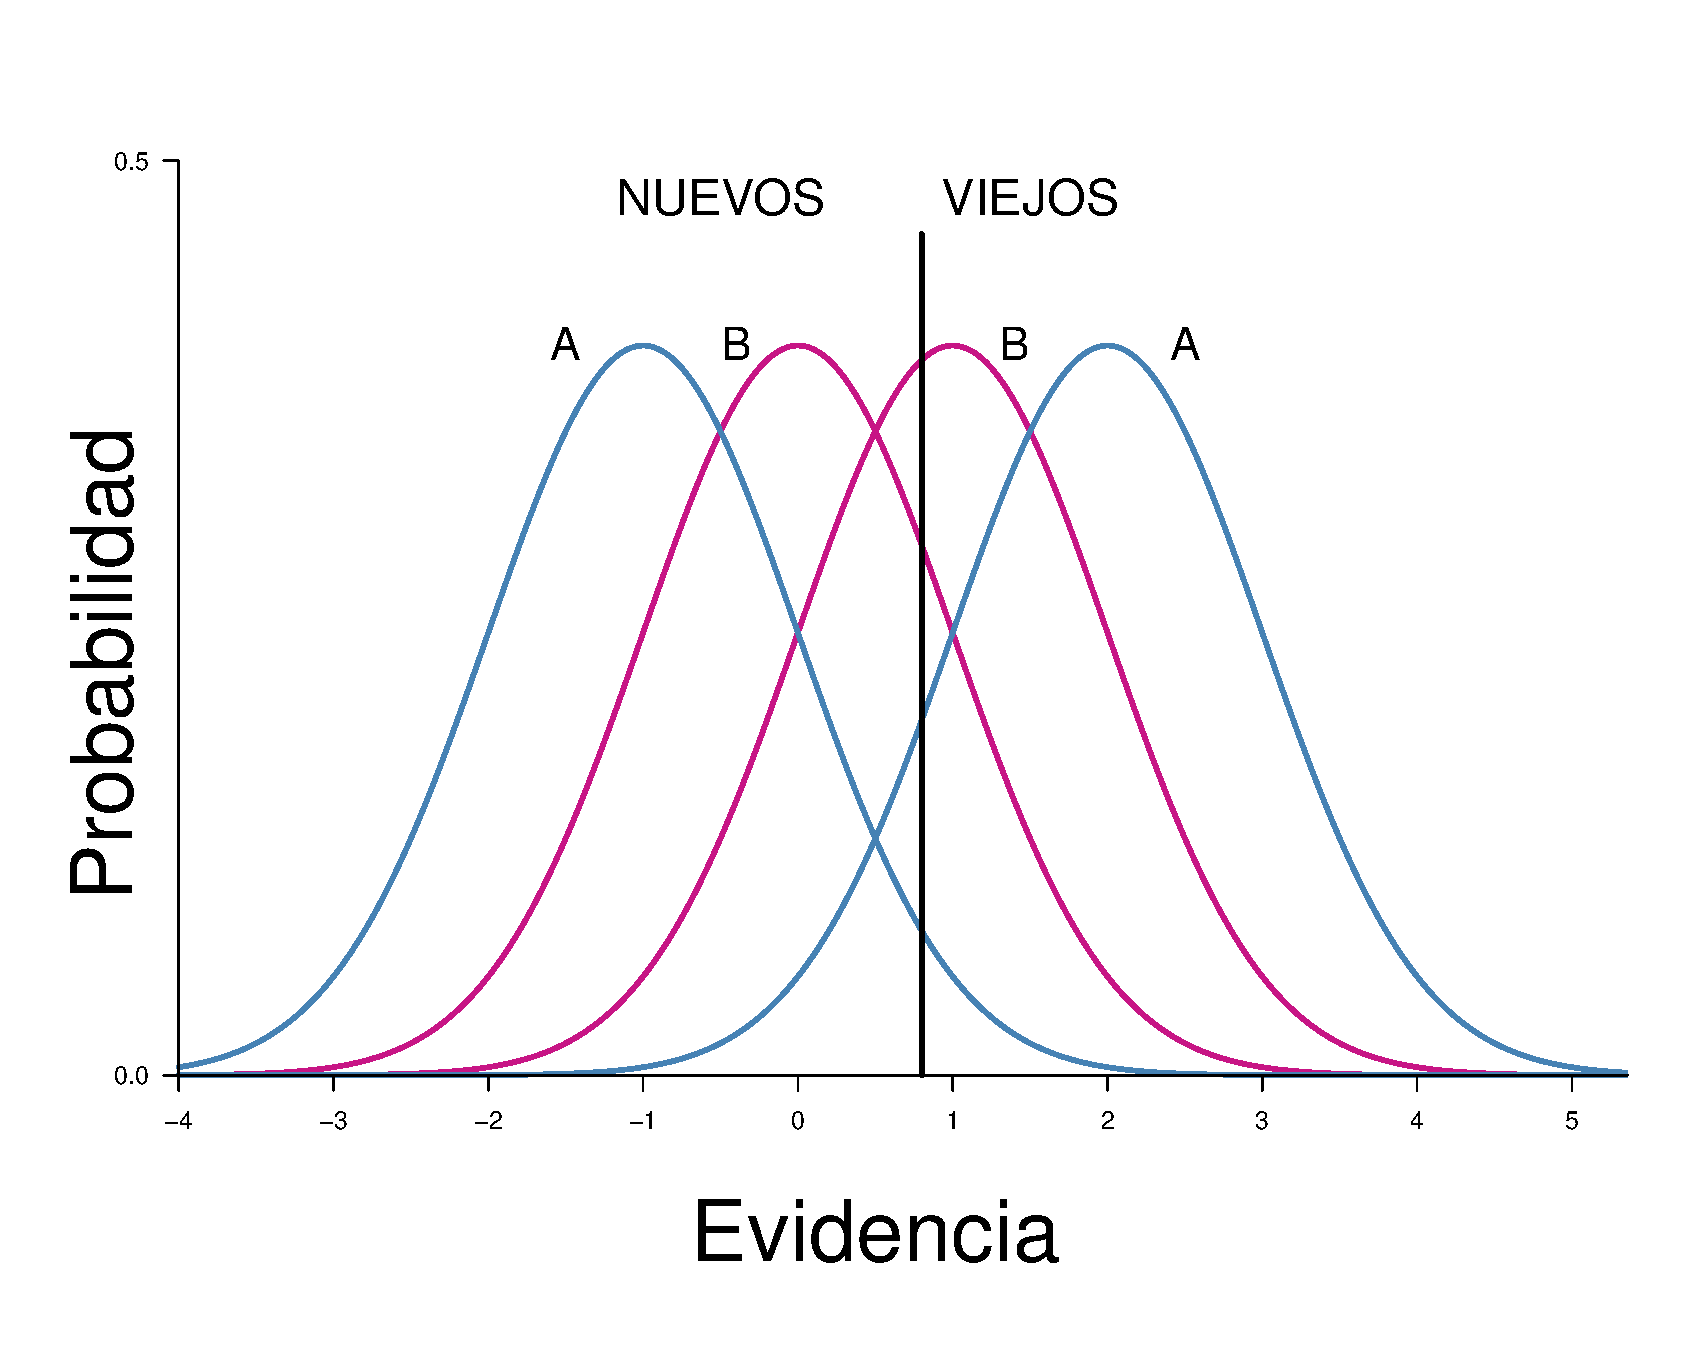
\includegraphics[width=0.7\textwidth]{Figures/EfectoEspejo_YesNo}
%\decoRule
\caption[Efecto Espejo en tareas de detección binarias]{Interpretación del patrón de respuestas reportado en tareas de reconocimiento Sí/No donde se presenta más de una clase de estímulos, ($FA(A) < FA(B) < H(B) < H(A)$), asumiendo que los participantes responden con base en un sólo criterio de elección.}
\label{fig:Ejem_Espejo_YesNo}
\end{figure}

El patrón de respuestas identificado en este tipo de tareas sugiere que las cuatro distribuciones se despliegan sobre el eje de evidencia tal y como se muestra en la Figura~\ref{fig:Ejem_Espejo_YesNo}: tomando la SDT como marco de referencia, las tasas reportadas de Falsas Alarmas y Hits para las clases A y B reflejan el área de las distribuciones de ruido y señal que caen por encima del criterio. La figura presenta un ejemplo ideal, donde las distribuciones Nuevas no sólo reflejan el órden de las distribuciones Viejas, sino que también mantienen la misma distancia entre sí.\\

\item \underline{Efecto Espejo con Escalas de Confianza}\\

En estudios de memoria de reconocimiento donde se comparan los puntajes de confianza emitidos entre dos clases de estímulos A y B, se encuentra la siguiente relación:\\

\begin{center}
$P(NuevoA) < P(NuevoB) < P(ViejoB) < P(ViejoA)$\\
\end{center}
\begin{center}
donde $P$ es el puntaje \textbf{promedio} asignado a los estímulos Nuevos y Viejos de cada clase de estímulo $A$ y $B$, en Escalas de Confianza donde los valores más altos señalan una mayor confianza en los juicios \textit{Viejo} y los valores más bajos, en \textit{Nuevo} (Glanzer y cols., \citeyear{Glanzer1993}).\\
\end{center}

\begin{figure}[h]
\centering
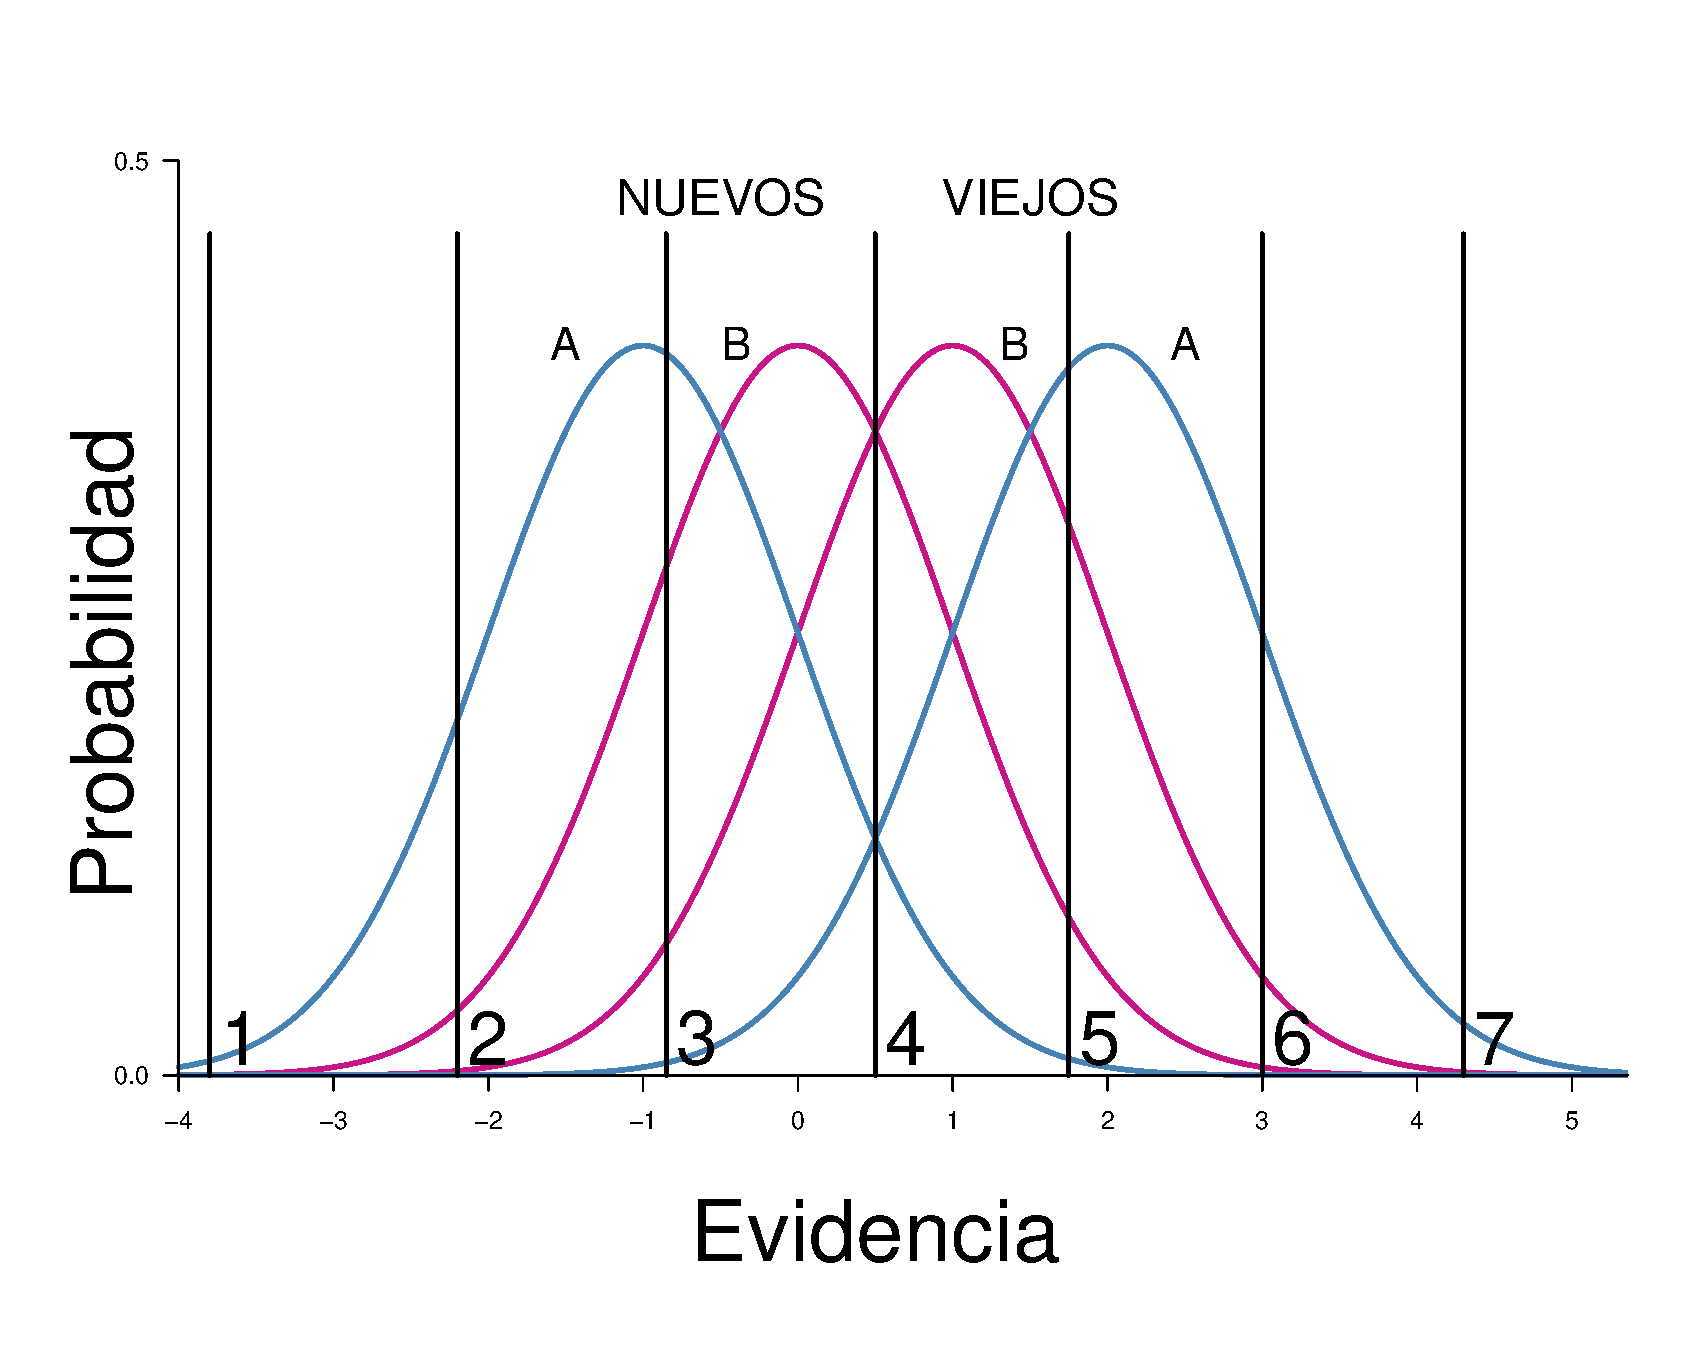
\includegraphics[width=0.7\textwidth]{Figures/EfectoEspejo_Puntajes}
%\decoRule
\caption[Efecto Espejo en tareas de detección con Escala de Confianza]{Interpretación del patrón de respuestas reportado en tareas de reconocimiento con Escala de Confianza, con más de una clase de estímulos ($P(NuevoA) < P(NuevoB) < P(ViejoB) < P(ViejoA)$). Asumiendo que los participantes utilizan los mismos sub-criterios de elección para todos los ensayos, el promedio de los puntajes asignados a cada subconjunto de estímulos resultan consistentes con el Efecto Espejo reportado en tareas binarias.}
\label{fig:Ejem_Efecto_Punt}
\end{figure}

De acuerdo con la SDT clásica (McNicol, \citeyear{McNicol2, McNicol5}), se asume que los participantes sitúan múltiples criterios de elección sobre el eje de evidencia para decidir qué puntaje de confianza emitirán para cada estímulo presentado, dependiendo cuál sea el último en ser rebasado por la \textit{familiaridad} evaluada. La Figura~\ref{fig:Ejem_Efecto_Punt} ilustra cómo esta idea y la representación del Efecto Espejo es compatible con el patrón encontrado en términos de los puntajes promedios asignados a los estímulos pertenecientes a cada una de las cuatro distribuciones. Las distribuciones de la clase A, que ocupan los valores más extremos del eje de evidencia, obtienen puntajes promedio más extremos que las distribuciones de clase B.\\

%\item \underline{Efecto Espejo en Tareas de Elección forzada entre dos alternativas}\\

%Como se mencionó previamente, en las Tareas de Elección forzada de $m$ Alternativas se presenta a los participantes en cada ensayo un número $m$ de estímulos, de los cuales $m-1$ contienen Ruido y sólamente $1$, la Señal.\\

%En el caso particular de los estudios en Memoria de Reconocimiento que proporcionan evidencia sobre la prevalencia y consistencia del Efecto Espejo, se refieren tareas de Elección Forzada de 2 alternativas. En dichos experimentos, se presenta a los participantes varias parejas conformadas por uno de los posibles estímulos con Señal ($ViejoA$ o $ViejoB$) y uno con Ruido ($NuevoA$ o $NuevoB$), siendo su tarea elegir cuál de estos dos estímulos le fue presentado durante la fase de estudio. De tal forma que en este tipo de estudios hay cuatro posibles tipos de parejas a presentar a los participantes en cada ensayo, (las \textit{parejas de comparación estándar}):\\

%\begin{itemize}
%\item Señal A VS Ruido A  (o ViejoA VS NuevoA)\\
%\item Señal A VS Ruido B (o ViejoA VS NuevoB)\\
%\item Señal B VS Ruido A (o ViejoB VS NuevoA)\\
%\item Señal B VS Ruido B (o ViejoB VS NuevoB)\\
%\end{itemize}

%En tareas de elección forzada entre 2 alternativas donde se incluyen las parejas de comparación estándar ya descritas, la evidencia a favor del Efecto Espejo se reporta a partir de las siguientes relaciones:\\

%\begin{center}
%$P(ViejoB, NuevoB) < P(ViejoB,NuevoA)$\\
%y\\
%$P(ViejoA, NuevoB) < P(ViejoA,NuevoA)$\\
%\end{center}
%\begin{center}
%donde $P$ implica la proporción de veces que el primer elemento de cada paréntesis es elegido sobre el segundo, cuando se solicita a los participantes que señalen el estímulo que se les haya presentado en la fase de estudio, \citep{Glanzer1993}.\\
%\end{center}

%Al interpretar los datos obtenidos en este tipo de tareas se asume que los participantes responden en cada ensayo eligiendo el estímulo con el valor más alto, en términos de su ubicación sobre el eje de decisión. Las parejas de comparación estándar formadas en experimentos que presentan evidencia a favor del Efecto Espejo están compuestas por un estímulo extraído de alguna de las distribuciones de estímulos Viejos y un estímulo proveniente de una distribución de estímulos Nuevos. De acuerdo con la representación gráfica de la localización de las cuatro distribuciones (ver Figura~\ref{fig:Ejem_EfectoEspejo}), existe una mayor distancia entre la distribución de estímulos Nuevos A (la distribución en el extremo izquierdo) y cualquiera de las dos distribuciones de estímulos Viejos, que entre estas y la distribución de estímulos Nuevos B (la segunda distribución de izquierda a derecha). Así, el patrón de respuestas reportado en este tipo de estudios hace sentido a la luz del orden en que se despliegan las cuatro distribuciones subyacentes: los participantes aciertan en mayor proporción -pues eligen el estímulo Viejo- en las parejas compuestas por un estímulo Nuevo A, ya que la distribución correspondiente se encuentra más alejada -y es por tanto, más discriminable- de las distribuciones de estímulos Viejos.\\

%Como un control adicional, en este tipo de experimentos se incluyen dos parejas adicionales (denominadas \textit{parejas de comparación nula}), que se componen por estímulos A y B, del mismo mismo tipo:\\

%\begin{itemize}
%\item Señal A VS Señal B (o ViejoA VS ViejoB)\\
%\item Ruido A VS Ruido B (o NuevoA VS NuevoB)\\
%\end{itemize}

%Mientras que en las elecciones observadas entre las parejas de comparación estándar se interpretan en términos de las distancias entre las distribuciones de estímulos Viejos y las distribuciones de estímulos Nuevos, las parejas de comparación nula proporcionan información acerca de la separación entre las distribuciones del mismo tipo de ensayo, pero diferente clase de estímulo. Si las respuestas de los participantes son consistentes con la representación gráfica del Efecto Espejo, se espera encontrar que:\\

%\begin{center}
%$P(ViejoA, ViejoB) > 0.5$\\
%y\\
%$P(NuevoB, NuevoA) > 0.5$\\
%\end{center}
%\begin{center}
%donde nuevamente $P$ representa la proporción de veces que se eligió el primer elemento de cada paréntesis como aquel que fue presentado anteriormente y $0.5$ señala la proporción que se esperaría encontrar si se asumiera que los participantes responden al azar, \citep{Glanzer1993}.\\ 
%\end{center}

%El punto clave detrás de la interpretación de las elecciones observadas en las parejas de comparación nula es que están compuestas por dos estímulos que representan el mismo estado -que al elegir cualquiera de estos el participante estaría cometiendo el mismo tipo de acierto o error- y, que en teoría, deberían ser elegidos por los participantes con la misma probabilidad (con proporciones cercanas al azar, $0.5$). Sin embargo, si la representación gráfica del Efecto Espejo es un reflejo apropiado de la ejecución de los participantes en este tipo de tareas, se espera encontrar una preferencia hacia la elección de los estímulos que provengan de la distribución más orientada hacia la derecha sobre el eje de evidencia. Por ejemplo, en el caso de las parejas de comparación nula compuestas por dos estímulos Nuevos A y B, se espera que los participantes elijan con una proporción superior al azar a los estímulos B, puesto que provienen de una distribución que cubre valores más altos sobre el eje de la evidencia que la distribución Nuevos A, \citep{Glanzer1993}.\\

\end{itemize}

En un inicio, los patrones de respuestas del ahora llamado Efecto Espejo fueron reportados en la literatura en memoria de reconocimiento como Efecto de Frecuencia de las Palabras (Schulman, \citeyear{Schulman1967}), ya que fueron encontrados por primera vez en estudios donde las clases entre las cuales se comparaba el desempeño de los participantes estaban compuestas por palabras \textit{poco comúnes} y palabras \textit{muy comunes}, de acuerdo a la frecuencia con que se usan (Kucera y Francis, \citeyear{Kucera1967}). Dichos estudios, realizados con diferentes protocolos experimentales (Glanzer y Bowles, \citeyear{Glanzer1976}; Bowles y Glanzer, \citeyear{Bowles1983}; Glanzer y Adams, \citeyear{Glanzer1990}), demostraron consistentemente que las palabras poco comúnes eran reconocidas con mayor precisión, tanto como Nuevas como Viejas (clase A), y que las palabras comúnes se confundían con mayor facilidad (clase B). No fue hasta que se demostró que los mismos patrones de respuesta aparecen a lo largo de una gran variedad de estudios donde las clases A y B son definidas en función a distintos factores -manipulando variables tales como la complejidad, la ortografía o la veracidad de los enunciados presentados, o bien, presentando estímulos cuyas características se sabe tienen una influencia en la precisión con que se les reconoce en presentaciones posteriores, como palabras con significado concreto (A) vs abstracto (B), imágenes (B) vs palabras (A), o rostros comúnes (B) vs rostros poco comúnes (A), entre otras (Glanzer y cols., \citeyear{Glanzer1993}; Greene, \citeyear{Greene1996}; Glanzer, Kim y Adams, \citeyear{Glanzer1998})-, que se comenzó a hablar del Efecto Espejo como una regularidad general, propia de la memoria de reconocimiento (Allen y Garton, \citeyear{Allen1968}; Glanzer y cols., \citeyear{Glanzer1993}).\\

\subsection{Relevancia, implicaciones e interpretaciones}\\

A primera vista, el patrón de respuestas identificado como Efecto Espejo podría parecer trivial: si sabemos que la principal diferencia entre las clases de estímulos presentadas en este tipo de estudios es la precisión con que sus elementos son reconocidos al presentarse más de una vez -siendo la clase A más fácil de reconocer que la clase B-, tiene sentido esperar que los participantes tengan un mejor desempeño general (más aciertos y menos errores) en la clase A. Sin embargo, al interpretar las tasas de ejecución observadas bajo el marco de la SDT, no parece claro por qué debería haber más de una distribución de ruido (como sugieren las diferencias encontradas entre las Falsas Alarmas registradas por cada clase), en tanto que en el contexto de la memoria de reconocimiento, se trata de elementos que no han sido presentados y deberían resultar igualmente \textit{familiares} -o a efectos prácticos, \textit{desconocidos}-.\\

Existen dos grandes formas en que el Efecto Espejo ha sido abordado en la literatura en memoria de reconocimiento:\\

\begin{enumerate}
\item Como reflejo de procesos cognitivos que subyacen a la ejecución de los participantes en tareas de reconocimiento (tanto en la fase de estudio, como en la fase de reconocimiento).\\

\item Como evidencia de que los modelos de memoria derivados de la SDT no describen adecuadamente el actuar de los mecanismos involucrados en la Memoria de Reconocimiento.\\
\end{enumerate}

Dentro de los modelos y teorías desarrollados para dar cuenta de lo que el Efecto Espejo podría estar sugiriendo acerca del funcionamiento de la memoria de reconocimiento se distinguen varias aproximaciones.\\

Una primera forma de interpretar el Efecto Espejo -y probablemente la más sencilla de todas- apela a las estrategias de respuesta \textit{deliberadamente} empleadas por los participantes. Este tipo de explicaciones se sustentan en el hecho de que las discrepancias entre las tasas de Falsas Alarmas desaparecen cuando se solicita explícitamente a los participantes que \textit{no adivinen} su respuesta (Greene, \citeyear{Greene1996}). Por ejemplo, la hipótesis de Distribución de las Respuestas supone que los participantes asumen por \textit{default} que la cantidad de estímulos Viejos y Nuevos a presentárseles durante el experimento es la misma y en consecuencia, modulan la cantidad de respuestas afirmativas que emiten. Este tipo de explicaciones implican también que los participantes pueden distinguir entre las dos clases de estímulos presentadas, de forma que, dado que los elementos Viejos de la clase A se identifican con mayor precisión ($Hits(A) > Hits(B)$), \textit{acumulan} una cantidad grande de respuestas afirmativas que compensan restringiendo la emisión de juicios afirmativos en los ensayos donde se les muestra estímulos de la misma clase que no contienen la Señal, reduciendo en consecuencia la tasa de Falsas Alarmas registrada para la clase A ($F.Alarmas(A) > F.Alarmas(B)$) (Greene, \citeyear{Greene1996}).\\

Un problema evidente con esta primera aproximación es que viola uno de los elementos clave detrás de la interpretación del Efecto Espejo como una fenómeno significativo y consistente en memoria de reconocimiento: el supuesto de que los participantes responden a partir de un sólo conjunto de criterios de elección que utilizan indistintamente entre los estímulos de clase A o B. En otras palabras, este tipo de explicaciones sólo permitirían dar cuenta de experimentos donde las clases A y B son fáciles de distinguir entre sí y dejan fuera el resto de los experimentos en que se ha encontrado evidencia del Efecto Espejo, sin que los participantes sepan que están siendo evaluados a traves de más de una clase de estímulos (Glanzer y cols., \citeyear{Glanzer1998}).\\

Una segunda aproximación implica asumir que las clases de estímulos empleadas en estos estudios difieren en el efecto que tienen sobre los procesos superiores involucrados en las tareas de reconocimiento. En otras palabras, este segundo conjunto de explicaciones asume que cada clase de estímulos A y B es procesada de manera distinta por los participantes. Como uno de los ejemplos más representativos de este tipo de explicaciones se encuentra la Teoría de Atención/Verosimilitud (Glanzer y cols., \citeyear{Glanzer1993}). Dicha teoría funciona como un modelo de muestreo de rasgos que se asume que todos los estímulos a presentar están compuestos por un número fijo de rasgos ($N$), de los cuales, algunos se presentan \textit{marcados} desde su primera aparición como \textit{rasgos familiares} ($p(new)$) y otros son marcados como tales una vez que se interactúa con ellos ($p(new) + [\alpha(i)* (1-p(new))]$). Esta teoría asume que la diferencia fundamental entre  las clases de estímulos probadas ($i$) es que elicitan distintos gradientes de atención que van a repercutir en el número de rasgos atendidos (\textit{muestreados}) por los participantes ($n(i)$) dentro de $N$, definiendo una \textit{tasa de marcaje} propia de cada clase ($\alpha(i)$).\\

\pagebreak
En otras palabras, el proceso mediante el cual se explica el Efecto Espejo de acuerdo a la Teoría de Atención/Verosimilitud es el siguiente:\\

\begin{enumerate}
\item Todos los estímulos están compuestos por una cantidad $N$ de rasgos.\\

\item Todos los estímulos comienzan con una cierta proporción de rasgos marcados como \textit{conocidos}.
\begin{center}
$p(A,nuevo) = p(new)$\\
$p(B,nuevo) = p(new)$\\
donde la cantidad de rasgos marcados inicialmente es la misma en las clases A y B.\\
\end{center}

\item A y B difieren en el número de rasgos que los participantes muestrean al interactuar con cada estímulo.
\begin{center}
$n(A) > n(B)$\\
La clase A es más atendida que B.\\
\end{center}

\item De acuerdo con $n(i)$, A y B tienen su propia tasa de muestreo.
\begin{center}
$\alpha(A) = \frac{n(A)}{N}$\\
$\alpha(B) = \frac{n(B)}{N}$\\
donde si $n(A) > n(B)$ entonces, $\alpha(A) > \alpha(B)$\
\end{center}

\item Al interactuar con los estímulos en la fase de estudio, los participantes muestrean cierto número de rasgos y marcan aquellos que no lo estén con anterioridad, ($\alpha(i)*(1-p(new))$).\\

\item En la fase de reconocimiento, los estímulos presentados previamente tienen una mayor proporción de rasgos marcados que los estímulos nuevos:
\begin{center}
$p(A,viejo) = p(new) + [\alpha(A)*(1-p(new))]$\\
$p(B,viejo) = p (new) + [\alpha(B)*(1-p(new))]$\\
\end{center}
\end{enumerate}

De acuerdo con la Teoría de Atención/Verosimilitud, los participantes registran sus respuestas en la fase de reconocimiento con base en la cantidad de rasgos \textit{marcados} muestreado ($x$). La probabilidad de observar cierto valor de $x$ se describe en función a una distribución binomial con probabilidad $p(i,j)$ (donde $i$ es la clase A o B y $j$ es el tipo de estímulo: nuevo o viejos), para el total de observaciones $n(i)$ registradas en función a la clase del estímulo. Es decir:

\begin{center}
$p(x|p(i,j),n(i))$\\
\end{center}

Al observar una cantidad $x$ de rasgos marcados, los participantes emiten el juicio de reconocimiento que corresponda a dicha evidencia con mayor probabilidad, computando una razón de verosimilitudes (Glanzer y cols., \citeyear{Glanzer1993}; Hintzman, \citeyear{Hintzman1994}; Glanzer, Hilford y Maloney, \citeyear{Glanzer2009}; Hilford, Maloney, Glanzer y Kim, \citeyear{Hilford2015}). De acuerdo con esta teoría, el Efecto Espejo se explica por medio de la siguiente relación:

\begin{center}
$p(x|p(A,nuevo),n(A)) < p(x|p(B,nuevo),n(B)) < p(x|p(B,viejo),n(B)) < p(x|p(A,viejo),n(A))$\\
\end{center}

En la Teoría de Atención/Verosimilitud el elemento clave para explicar las diferencias en el desempeño de los participantes entre A y B es la atención elicitada por cada clase, y el número de rasgos muestreados en consecuencia ($n(i)$). Esto resuelve el problema de las discrepancias entre las tasas de Falsas Alarmas de la siguiente forma: aunque A y B contienen el mismo número de rasgos marcados en su primera presentación ($p(A,nuevo) = p(B,nuevo)$), el número de elementos muestreados es mayor en la condición A ($n(A) > n(B)$) y por tanto, hay una mayor probabilidad de extraer más rasgos marcados que en B ($p(x|p(A,nuevo),n(A)) < p(x|p(B,nuevo),n(B))$).\\

Pese al conjunto de experimentos desarrollados para probar la solidez de la Teoría de Atención/Verosimilitud mediante la manipulación de distintas variables experimentales que deberian tener un impacto sobre los parámetros del modelo (por ejemplo, restringiendo el tiempo de estudio y/o de respuesta para modificar $n(i)$ en cada fase) y evaluando la precisión con que el modelo predice y explica los datos encontrados (Glanzer y cols., \citeyear{Glanzer1993}; Kim y Glanzer, \citeyear{Kim1993}; Glanzer, Adams e Iverson, \citeyear{Glanzer1991}), la Teoría de Atención/Verosimilitud ha sido fuertemente criticada en relación a dos grandes factores: 1) la teoría está compuesta por parámetros y supuestos innecesariamente complejos que le restan validez ecológica y 2) la teoría asume que los participantes tienen acceso a información completa sobre la estructura de la tarea y son capaces de utilizarla para realizar cómputos altamente demandantes (Hintzman, \citeyear{Hintzman1994}; Murdock, \citeyear{Murdock1998}; DeCarlo, \citeyear{DeCarlo2007}).\\

Una tercera forma de interpretar el Efecto Espejo es de manera consistente con la aplicación de la SDT al análisis de las tareas de reconocimiento: asumiendo que los participantes registran sus respuestas en función a la evidencia que evalúan en cada ensayo (\textit{la fuerza de memoria} o \textit{familiaridad} contenida en el eje de evidencia), sin necesidad de recurrir a ningún tipo de cómputo adicional (Hintzman, \citeyear{Hintzman1994}). Bajo esta perspectiva, la única diferencia que existe entre las clases A y B -sin importar si pueda justificarse el por qué de ella- es la \textit{fuerza de memoria} que contienen, o bien qué tan familiares resultan para los participantes. Por ejemplo, en los estudios donde se usan distintos niveles de \textit{Palabras frecuentes} para delimitar las clases de estímulos a comparar, las palabras poco comúnes parecen ser más fáciles de recordar y reconocer (A) y las palabras comúnes parecen confundirse con mayor facilidad (B). De acuerdo a este tipo de explicaciones, las palabras comúnes Nuevas (B,Nuevo) tienen un mayor grado de familiaridad que los estímulos Nuevos poco comúnes (A,Nuevo), por lo que la separación de las dos distribuciones de estímulos Nuevos tiene sentido. A su vez, dado que las palabras poco comúnes son más salientes, se asume que se les presta más atención y terminan adquiriendo un mayor nivel de familiaridad cuando se les presenta por segunda vez que las palabras comúnes, lo que termina explicando el orden en que se presentan las distribuciones de estímulos Viejos (Glanzer y cols., \citeyear{Glanzer1993}).\\

En una dirección distinta, se encuentran las interpretaciones del Efecto Espejo que tienden a tomarle como evidencia para desacreditar el uso de la SDT para estudiar del fenómeno de la memoria de reconocimiento. Por ejemplo, un primer conflicto evidente en la interpretación del Efecto Espejo es que no siempre parece claro por qué una de las clases de estímulos a probar debería resultar \textit{más familiar} (A) que la otra (B) desde que se presenta en la fase de estudio. Aún cuando este tipo de explicaciones se sostiene de manera intuitiva para entender los resultados encontrados en estudios donde A y B se componen de palabras poco comúnes y comúnes, cuando se intenta añadir una tercer clase C, compuesta por palabras \textit{raras}, los resultados encontrados no son consistentes con lo que la interpretación del Efecto Espejo sugeriría (Rao y Proctor, \citeyear{Rao1984}; Wixted, \citeyear{Wixted1992}). En general, se esperaría que la nueva clase C añadiera dos distribuciones más sobre el eje de evidencia, que se agregarían hacia los extremos inferior y superior del mismo. Sin embargo, este no parece ser el caso.\\

Por último, se encuentran los trabajos orientados al desarrollo y evaluación de distintos modelos de detección de señales que difieren en la naturaleza que se asume tienen las distribuciones subyacentes a la tarea. Por ejemplo, asumiendo distintos tipos de distribuciones (Glanzer y cols., \citeyear{Glanzer1993}, \citeyear{Glanzer2009}) o bien, fomentando el abordaje del problema desde la perspectiva de los modelos de mezclas en detección de señales (DeCarlo, \citeyear{DeCarlo2002} ,\citeyear{DeCarlo2007}).\\

\section{Planteamiento del problema}

Como se describió en la sección anterior, el Efecto Espejo es un fenómeno empírico reportado en estudios de memoria de reconocimiento desarrollados bajo el marco de la SDT. Su consistencia a lo largo de diversos procedimientos y variables impulsó el desarrollo de distintos tipos de interpretaciones, tanto en términos de lo que podría sugerir sobre cómo opera la memoria de reconocimiento, como de la evaluación del uso del modelo de detección de señales como marco para describir la ejecución de los participantes en este tipo de tareas.\\

En contraste con la amplia variedad de propuestas desarrolladas para dar cuenta del Efecto Espejo como un fenómeno intrínseco a la Memoria de Reconocimiento, es importante señalar que dicho fenómeno no ha sido estudiado ni reportado en ningún otro tipo de tareas de detección.\\

Evaluar la generalizabilidad del Efecto Espejo a otras áreas de aplicación de la SDT se considera importante en tanto que 1) provería un contexto más amplio para interpretar el Efecto Espejo como una regularidad derivada de los supuestos establecidos por la SDT y no como un fenómeno particular de la memoria de reconocimiento y los procesos cognitivos involucrados, y 2) permitiría evaluar la pertinencia de la aplicación del modelo de detección de señales para interpretar los resultados obtenidos en este tipo de tareas en memoria de reconocimiento.\\

El trabajo de tesis aquí presentado no se preocupa en evaluar de forma alguna las propuestas teóricas y formales desarrolladas para dar cuenta del Efecto Espejo como un fenómeno inherente a la memoria de reconocimiento. El objetivo del trabajo de investigación realizado es meramente el de explorar la existencia de los patrones de respuesta identificados como Efecto Espejo en una tarea de detección ajena al marco de la memoria de reconocimiento. Para ello, se propuso trabajar con una tarea de detección perceptual que emula las condiciones básicas de las tareas de reconocimiento donde dicho fenómeno ha sido reportado, construyéndose las clases de estímulos A y B a partir de la revisión de la literatura en ilusiones ópticas para garantizar que estas difirieran en su discriminabilidad ($d'$).\\

 
% Chapter Template

\chapter{Método} % Main chapter title

\label{Cap_Exp} % Change X to a consecutive number; for referencing this chapter elsewhere, use \ref{ChapterX}

%----------------------------------------------------------------------------------------
%	SECTION 1
%----------------------------------------------------------------------------------------
\section{Planteamiento general}

%Se propone buscar evidencia del Efecto Espejo en una tarea fuera de Memoria de reconocimiento.
Al tratarse de un fenómeno exclusivamente reportado, estudiado e interpretado dentro de la literatura en Memoria de Reconocimiento, existe una tendencia a explicar el Efecto Espejo -las diferencias en la ejecución de los participantes entre las clases de estímulos contenidos en el experimento- apelando a posibles discrepancias en el procesamiento superior de los mismos durante la fase de estudio (por ejemplo, la atención, la recolección de rasgos para su futuro reconocimiento, etc.). El interés principal de la investigación aquí reportada fue buscar evidencia de los patrones de respuesta reportados en estudios de Memoria de Reconocimiento en una tarea de detección ajena a dicha área.\\

%Encontrar evidencia del Efecto Espejo en otra área, podría sugerir que el Efecto Espejo es resultado del uso de SDT para comparar dos condiciones de discriminabilidad y no necesariamente de un fenómeno de Memoria per see.
Buscar evidencia del Efecto Espejo fuera del área de Memoria de Reconocimiento permite evaluar la posibilidad de que los patrones de respuesta reportados como parte del mismo sean producto de la aplicación de la SDT como marco para el análisis y comparación de la ejecución de los participantes entre clases de estímulos que difieren en su discriminabilidad y no necesariamente de una discrepancia en su procesamiento durante la fase de estudio.\\

%Se propone una tarea perceptual ya que carece de una fase de preparacion. Se trabaja con ilusiones opticas, dado que la literatura en ellas permite anticiparnos a la d' y proponer dos niveles de dificultad.
Se decidió trabajar con una tarea de detección perceptual por dos razones. La primera razón es que una tarea de este tipo implica un procedimiento más sencillo: los participantes deciden si la señal está o no presente en los estímulos mostrados sin haber interactuado con estos en una etapa previa. La señal a detectar se percibe en el estímulo, no se reconoce de la experiencia previa con el mismo. La segunda razón es que existe un cuerpo de literatura lo suficientemente amplio como para permitir la construcción de dos niveles de dificultad dentro de la tarea, específicamente, se revisó y trabajó con la literatura que aborda el fenómeno de las ilusiones ópticas.\\

\subsection{Objetivo}

%Buscar evidencia del efecto espejo en una tarea de detección perceptual.
Determinar si los patrones de respuesta identificados como parte del Efecto Espejo en Memoria de Reconocimiento aparecen también al comparar el desempeño de los participantes entre distintos niveles de discriminabilidad en una tarea de detección perceptual.\\

\section{Construcción de los Experimentos}

%5.	Jaeger, T., & Pollack, R. (1977). Effect of contrast level and temporal order on the Ebbinghaus circles illusion. Perception & Psychophysics. Vol 21 (1), 83-97.
%9.	Pressey, A. (1977). Measuring the Titchener circles and Delboeuf illusions with the method of adjustment. Bulletin of Psychonomic Society. Vol 10 (2), 118-120.
%Coren, S., & Girgus, J. (1978). Seeing is deceiving: The psychology of visual illusions. Hillsdale, NJ: Erlbaum.
%Titchener E B, 1901 Experimental Psychology: A Manual of Laboratory Practice volume I (London: MacMillan) (1901, page 169, figure 3)
%Robinson J O, 1972 The Psychology of Visual Illusion (London: Hutchinson Education)
%Rabin, J., & Adams, A. J. (1993). Size induction transcends the cardinal directions of color space. Perception, 22, 841–845.

%La tarea de detección consiste en identificar los ensayos donde el tamaño de dos círculos en pantalla es igual. Esta tarea tiene dos variaciones: En el Experimento 1, uno de los círculos a comparar es el círculo central de una ilusión de Ebbinghaus; En el Experimento 2, los dos círculos lo son. 
Se diseñó una tarea perceptual donde los participantes tenían que comparar el tamaño de dos círculos mostrados en pantalla y emitir una respuesta que señalara si los círculos tenían el mismo diámetro (señal) o no (ruido). Esta tarea se presentó en dos variaciones: En un primer caso, sólo uno de los círculos a comparar constituía el círculo central de una figura de Ebbinghaus (Experimento 1); En el segundo, ambos círculos aparecían como el componente central de una figura de Ebbinghaus distinta (Experimento 2).\\ 

%Descripcion de la Ilusión de Ebbinghausyhhhhhhhhhhvcf , la composición de la figura y cómo se explica.
La figura de Ebbinghaus -también conocida como Círculos de Titchner- está intrínsecamente relacionada con una ilusión óptica donde la percepción del tamaño de un elemento central es alterada por el contraste que tiene con elementos circundantes (la ilusión de Ebbinghaus). En la Figura~\ref{fig:Ebbinghaus} se presenta un par de ejemplos prototípicos de figuras con la ilusión de Ebbinghaus que demuestran las dos direcciones en que esta se puede presentar: la subestimación del tamaño de un estímulo (el círculo central) al estar rodeado por éstímulos más grandes (efecto de subestimación; figura izquierda), y la sobrestimación del tamaño de un estímulo rodeado por elementos de menor tamaño (efecto de sobrestimación; figura derecha); el diámetro de los círculos centrales en ambas figuras es el mismo. Esta ilusión perceptual suele explicarse como el reflejo de una tendencia en nuestro sistema a computar el tamaño de los objetos en función a su contraste con elementos similares en su entorno \parencite{Coren1971, Coren1974, Fockert2007}.\\

\begin{figure}[th]
\centering
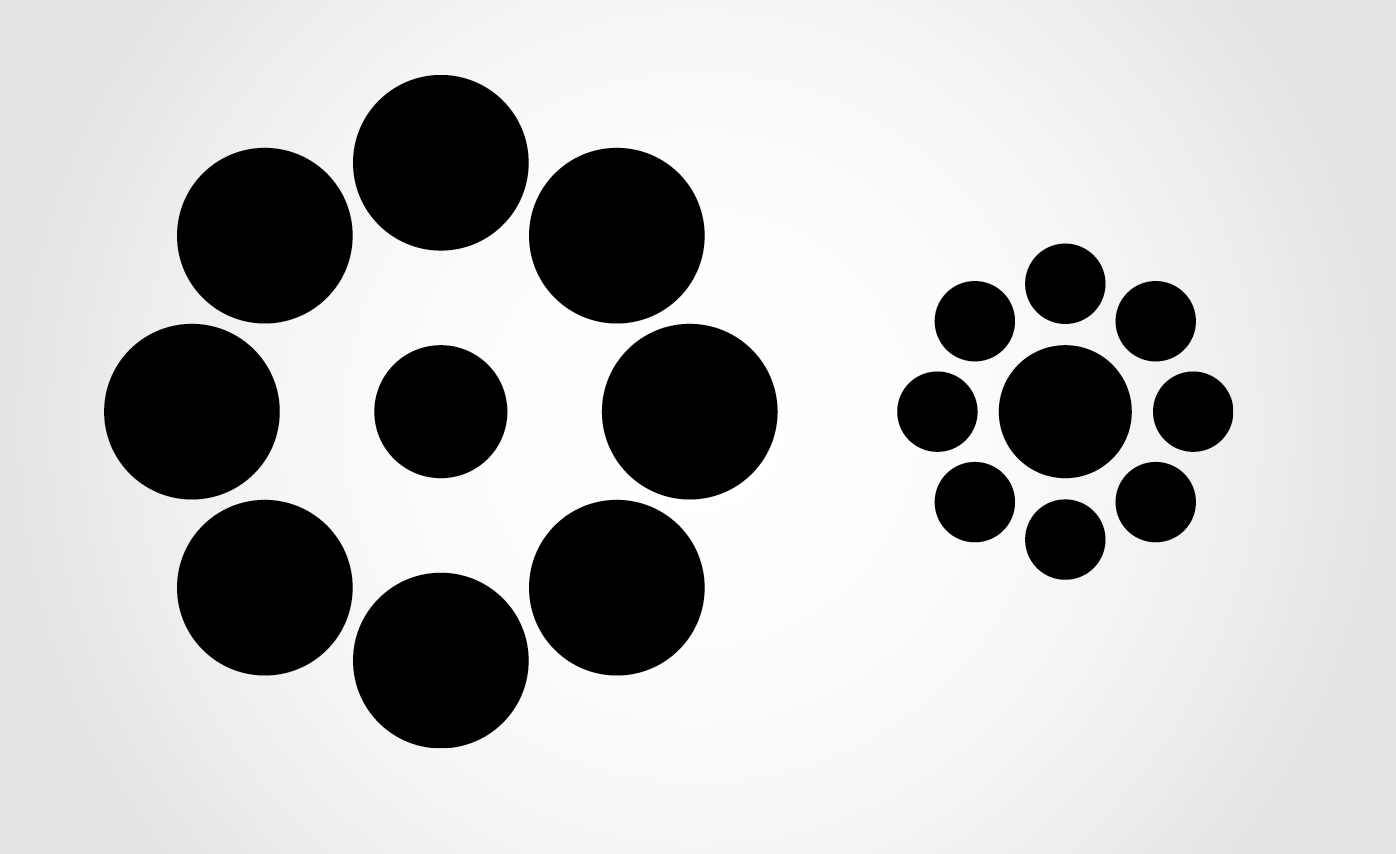
\includegraphics[width=0.55\textwidth]{Figures/Ebbinghaus} 
\decoRule
\caption[Ilusión de Ebbinghaus: Ejemplos]{Ejemplos prototípicos de la Ilusión de Ebbinghaus. Los círculos centrales de las dos figuras mostradas tienen el mismo diámetro, sin embargo, el círculo central de la figura izquierda tiende a percibirse como más pequeño (efecto de subestimación) y el círculo central de la figura derecha suele percibirse como más grande (efecto de sobrestimación) por el contraste que ambos círculos guardan con los círculos que les rodean.}
\label{fig:Ebbinghaus}
\end{figure}

%Factores o variables que han demostrado influir en la intensidad de la ilusión.
La intensidad de la ilusión de Ebbinghaus -qué tanto se aleja el tamaño estimado del tamaño real del círculo central- suele definirse como una función de las siguientes variables \parencite{Massaro1971, Girgus1972, Roberts2005}: 

\begin{itemize}
\item El tamaño de los círculos externos.
\item La distancia entre el círculo central y el halo de círculos externos.
\item El número de círculos externos.
\end{itemize}

%Descripción del procedimiento empleado por Massaro y Anderson para probar la influencia del numero de circulos externos y el tamaño de los mismos en la Ilusión de Ebbinghaus.
La Figura~\ref{fig:Ebb_Var} presenta los resultados obtenidos en un experimento donde se evaluó el efecto de dos de las variables antes mencionadas en la intensidad de la ilusión de Ebbinghaus \parencite{Massaro1971}. En dicho estudio, se construyeron 30 figuras de Ebbinghaus con un diseño factorial de 2x3x5: dos tamaños de círculo central (13 y 17 mm), tres niveles de \textit{'número de círculos externos'} (dos, cuatro y seis) y cinco tamaños diferentes de círculos externos (-8, -4, 0, 4 y 8 mm de diferencia respecto del diámetro del círculo central); la distancia entre el círculo central y los círculos externos se mantuvo constante para todas las figuras. La tarea de los participantes era elegir dentro de un set de 27 círculos diferentes (con diámetros de 8.5 a 21.5 mm en saltos de 0.5 mm), el círculo cuyo diámetro fuera más cercano al círculo central de la figura de Ebbinghaus presentada en cada ensayo. La Figura muestra el diámetro promedio elegido por los participantes como más cercano a los círculos centrales de las figuras de Ebbinghaus construidas (se promediaron los datos obtenidos para los dos tamaños de círculo central usados), a lo largo de los distintos niveles de número de círculos externos (en el eje de las abscisas) y por cada valor de diámetro de los círculos externos (en diferentes líneas). El efecto de las manipulaciones hechas parece claro: 1) Entre más círculos externos se incluyen en las figuras de Ebbinghaus, mayor es la intensidad de la ilusión, como señala la tendencia de las lineas a mostrar distancias cada vez mayores entre el promedio de los valores reales de círculo interno y la estimación hecha por los participantes; 2) la intensidad de la ilusión es mayor mientras mayor sea la diferencia entre el tamaño del círculo central y los círculos externos, como sugiere la distancia vertical entre cada una de las líneas, cuya dirección permite distinguir con claridad entre los efectos de sobreestimación y subestimación.\\

\begin{figure}[th]
\centering
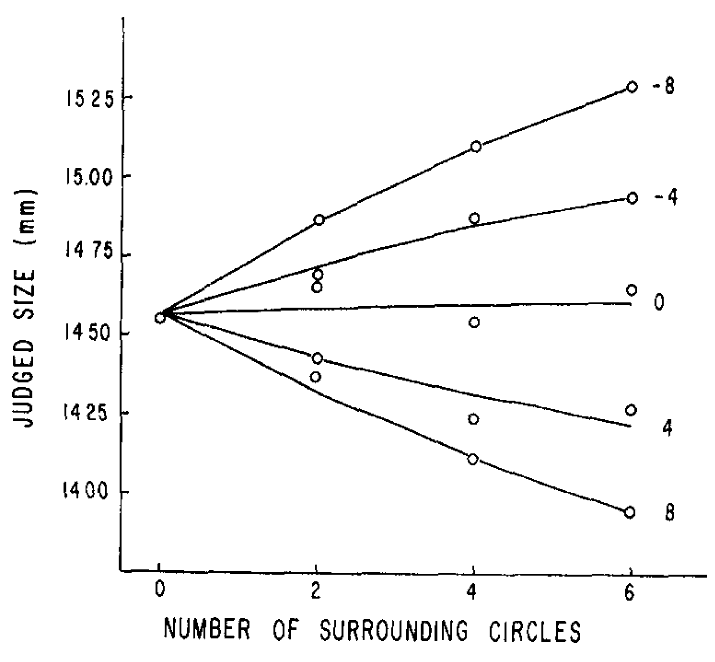
\includegraphics[width=0.55\textwidth]{Figures/Ebb_Variables} 
\decoRule
%\caption[Efecto del Numero y Tamaño de los círculos externos sobre la intensidad de la Ilusión de Ebbinghaus]{Se muestra el efecto que tienen el número de círculos externos incluídos en la ilusión de Ebbinghaus (eje x) sobre los fallos en la estimación del tamaño del círculo central (eje Y); se muestran con líneas diferentes los resultados obtenidos por ilusiones de Ebbinghaus donde los círculos externos diferían en tamaño del círculo central con los valores especificados. La figura fue extraída de la investigación conducida por \parencite{Massaro1971}; Figura 2}
\caption[Efecto del Número y Tamaño de los círculos externos en la intensidad de la Ilusión de Ebbinghaus]{Se presentan los resultados obtenidos en un experimento donde se manipuló el número y tamaño de los círculos externos de figuras de Ebbinghaus para evaluar su efecto sobre la intensidad de la ilusión perceptual evocada. La gráfica muestra el estimado del diámetro del círculo central de las figuras presentadas (promediando los datos obtenidos por todos los participantes y por los dos tamaños de círculo central usados: 13 y 17 mm), a través de los distintos niveles de número de círculos externos evaluados (eje de las abscisas) y por cada uno de los cinco tamaños de círculos externos utilizados (mostrados en líneas separadas). La tendencia de las líneas a alejarse del estimado promedio en ausencia de círculos externos -sin ilusión inducida- sugiere que a mayor número de círculos externos, mayor es la intensidad de la ilusión. La distancia vertical entre las líneas dibujadas parece indicar que la intensidad de la ilusión aumenta mientras mayor sea la diferencia entre el diámetro del círculo central y el de los círculos externos. \parencite{Massaro1971}.}
\label{fig:Ebb_Var}
\end{figure}

%Las condiciones de dificultad estarán determinadas por el número de círculos externos
Tomando en consideración los hallazgos reportados respecto de la influencia que tienen las variables inmersas en las figuras de Ebbinghaus sobre la ilusión perceptual asociada a las mismas \parencite{Massaro1971}, se decidió construir las dos condiciones de discriminabilidad para nuestra tarea de detección perceptual en búsqueda del Efecto Espejo, manipulando el número de círculos externos. Es decir, para que en la tarea de detección propuesta existiera una condición fácil -la \textit{clase A} con una $d'$ grande- se construyeron figuras de Ebbinghaus con \textit{pocos} círculos externos (2 o 3 círculos); y para la condición difícil -la \textit{clase B} con una $d'$ menor- se diseñaron figuras con \textit{muchos} círculos externos (7 u 8 círculos).\\ 

\subsection{Diseño de los Estímulos}

%En el experimento se trabajó con figuras de Ebbinghaus que promovieran efecto de subestimación Y sobrestimación del tamaño. 
En el diseño de las figuras de Ebbinghaus a utilizar en los experimentos propuestos se incluyeron los efectos de sobrestimación y de subestimación. Para ello se manejaron sólo dos tamaños de círculos externos, elegidos arbitrariamente de manera que fueran o más grandes que todos los tamaños de círculo central o más pequeños que la mayoría (5 cm y 1 cm).\\

%No se controló la distancia entre el círculo central y los círculos externos.
En ningún experimento se controló la distancia entre los círculos centrales y el halo de círculos externos. Los círculos externos fueron acomodados de acuerdo a los números de círculos externos considerados como parte de la condición difícil (siete y ocho), distribuyéndolos de manera uniforme y equidistante en torno al círculo central. Estos halos de siete y ocho círculos externos fueron usados como base para la construcción de los estímulos de la condición fácil (con dos o tres círculos externos), eliminando círculos y respetando la ubicación de los restantes. Este procedimiento se realizó para las figuras con efecto de subestimación y sobrestimación. Se procuró que en las figuras con dos círculos externos, estos estuvieran enfrentados en puntos opuestos del círculo central y en las figuras con tres círculos centrales, que rodearan al círculo central en ángulos de ciento veinte grados. La configuración de los halos de círculos externos resultantes permaneció constante para todos los tamaños de círculo central, haciendo que la distancia entre ambos elementos sea distinto para cada valor.\\

%El diámetro de los círculos centrales de las figuras de Ebbinghaus podía ser de 1 a 3 cm, en saltos de 0.5 cm
En ambos experimentos se utilizaron cinco valores para el tamaño de los círculos centrales (de 1 a 3 cm, en saltos de 0.5 cm). Cabe señalar que el diámetro elegido para los círculos externos en las ilusiones de sobrestimación (1 cm) es el mismo que el círculo central más pequeño. Sin embargo, esto no se considera un problema para la presente investigación porque la inclusión de los dos efectos (sobrestimación y subestimación) se hizo con la intención de prevenir la habituación y la fatiga de los participantes a la tarea, proveyendo a la misma de cierto dinamismo. El objetivo principal de la investigación realizada fue comparar el desempeño de los participantes entre las condiciones de discriminabilidad construidas con base en la literatura, y este tipo de figuras \textit{'anómalas'} se presentan de igual manera en ambas condiciones.\\

A continuación, se desarrolla con detalle la construcción de los estímulos y la distinción entre los tipos de ensayo (señal y ruido) aplicadas en cada uno de los dos experimentos llevados a cabo. Las especificaciones respecto al procedimiento y los controles realizados se explican con detalle más adelante.\\

\begin{itemize}
\item Experimento 1 : Circulo de referencia aislado vs Figura de Ebbinghaus.

%Los ensayos de la tarea de detección están compuestos por un círculo aislado constante del lado izquierdo, cuyo tamaño debe ser comparado con el círculo central de una figura de Ebbinghaus en el lado derecho de la pantalla.
En el Experimento 1, en cada ensayo se presentó una figura de Ebbinghaus (en la mitad derecha de la patalla) acompañada de un círculo de referencia aislado (del lado izquierdo) cuyo diámetro permanecía constante a lo largo del experimento ($2$ $cm$). En este experimento, la tarea de los participantes consistió en presionar la tecla \textit{'S'} cuando el círculo central de la figura de Ebbinghaus fuera del mismo tamaño que el círculo de referencia (la \textit{señal}) y la tecla \textit{'N'} cuando no (el \textit{ruido}). Los círculos a comparar se presentaban a la misma altura de la pantalla, 14 cm a la izquierda y 10 cm a la derecha del centro de esta.\\

%Desarrollo del diseño factorial de 5x2x2 utilizado para construir los estímulos del Experimento 1: 5 circulos centrales x 2 tipos de ilusion x 2 niveles de 'numero de circulos externos'
Las figuras de Ebbinghaus utilizadas en el Experimento 1 se diseñaron de acuerdo a un diseño factorial de 5x2x2, (Ver Figura~\ref{fig:Exp_1}). Se utilizaron cinco tamaños de círculo central que, partiendo del tamaño del círculo de referencia (2 cm; la combinación con la señal), se alejaban del mismo en saltos de 0.5 cm en ambas direcciones (i.e. Círculos más pequeños que la referencia, de 1 y 1.5 cm, y círculos más grandes que la referencia, de 2.5 y 3 cm de diámetro). Por cada uno de estos cinco tamaños de círculo central, se construyeron dos tipos de figuras de Ebbinghaus dependientes del tamaño de los círculos externos: grande (5 cm; efecto de subestimación) y pequeño (1 cm; efecto de sobrestimación). Y por último, por cada una de estas 10 combinaciones, se hicieron cuatro figuras diferentes de acuerdo a los niveles de \textit{'número de círculos externos'} propuestos por condición (2 y 3 círculos en la condición fácil; 7 y 8 círculos en la condición difícil). Esto nos deja con un subtotal de 20 figuras diferentes por condición y un total de 40 en todo el experimento.\\
 
%Los estímulos con ruido se presentaron 10 veces durante el experimento. Los estímulos con señal se presentaron con 40 repeticiones. La discrepancia en el número de repeticiones entre ambos tipos de estímulo se hizo para igualar la muesta de ensayos con señal y ensayos con ruido.
El conjunto de figuras de Ebbinghaus resultante contiene una mayor cantidad de estímulos con ruido (32 figuras con ruido; 16 por condición) que con señal (8 figuras con la señal; 4 por condición). Para igualar la cantidad de ensayos con señal y con ruido presentados a los participantes y preveer que la diferencia en su tasa de aparición pudiera sesgar su desempeño hacia la emisión de respuestas negativas, las figuras con señal diseñadas se repitieron un mayor número de veces que las figuras con ruido. Cada una de las 32 figuras de Ebbinghaus con ruido se presentó con diez repeticiones durante el experimento, mientras que las ocho figuras con señal tuvieron cuatro veces más repeticiones (40 en total). De esta forma, el experimento terminó compuesto por 320 ensayos con ruido y 320 ensayos con señal, 160 por cada condición de dificultad.\\

%Las repeticiones de cada figura aparecieron en cinco colores diferentes para prever la fatiga.
Los 640 estímulos contemplados en el Experimento 1 fueron presentados de manera aleatoria. Procurando evitar la fatiga de los participantes, las repeticiones de los estímulos diseñados se mostraron en cinco colores diferentes (Guinda, Anaranjado, Verde, Azul y Púrpura) en cantidades iguales (dos repeticiones de cada color para los estímulos con ruido y ocho para los estímulos con señal).\\

\item Experimento 2 : Figura de Ebbinghaus vs Figura de Ebbinghaus.

%En la tarea de detección, los participantes tenían que comparar el círculo central de dos figuras de Ebbinghaus que aparecían simultáneamente en la pantalla: una con círculos externos grandes (Efecto de subestimación)  y una con círculos externos pequeños (Efecto de sobrestimación).
En el Experimento 2 los participantes tenían que comparar el diámetro del círculo central de dos figuras de Ebbinghaus mostradas simultáneamente en pantalla y, al igual que en el Experimento 1, presionar la tecla \textit{'S'} cuando fueran del mismo tamaño (señal) y la tecla \textit{'N'} cuando no (ruido). Las parejas construidas estaban compuestas por una figura de Ebbinghaus con efecto de subestimación (con círculos externos grandes, de 5 cm de diámetro) y una figura con efecto de sobrestimación (con círculos externos pequeños, de 1 cm de diámetro). Los círculos centrales aparecían en pantalla a la misma altura, 15 cm a la izquierda y 11 cm a la derecha del centro de la pantalla.\\


%Se formaron cinco parejas con la Señal (cinco pares iguales de tamaño de círculo central) y cinco parejas con el ruido (cuatro cuyos círculos centrales diferían en 0.5 cm y una que difería en 1 cm).
La Figura~\ref{fig:Exp_2} ilustra el diseño de las figuras de Ebbinghaus utilizadas en el Experimento 2. A diferencia del Experimento 1, donde uno de los círculos a comparar era constante, en el Experimento 2 se varió el diámetro de los dos círculos a comparar. Para ello se ello se utilizaron los mismos cinco tamaños de círculo central (de 1 a 3 cm en saltos de 0.5 cm) y por lo tanto, con cinco combinaciones posibles para las Parejas-señal. Así mismo, se formaron cinco Parejas-ruido juntando arbitrariamente valores de círculo central que guardasen una diferencia de 0.5 cm entre sí -1 vs 1.5; 1.5 vs 2; 2 vs 2.5 y 2.5 vs 3 cm- con una quinta pareja con una diferencia de 1 cm entre los valores de círculo central intermedios -1.5 cm vs 2.5 cm-. Por cada una de estas 10 parejas, se crearon cuatro variaciones por condición, de acuerdo con las combinaciones posibles de niveles de \textit{'número de círculos externos'} (2 círculos externos a ambos lados, 3 círculos externos a ambos lados, 2 en izquierdo y 3 en derecho, y 3 en izquierdo y 2 en derecho en la condición fácil; 7 círculos externos a ambos lados, 8 círculos externos ambos lados, 7 círculos del lado izquierdo y 8 en el derecho y 8 círculos en el lado izquierdo y 7 en el derecho en la condición difícil). En total, el Experimento 2 estuvo compuesto por 80 parejas diferentes de figuras de Ebbinghaus cuyos círculos centrales debían compararse, 40 con la señal y 40 con el ruido y 20 de cada uno por condición.\\

%Cada pareja diseñada se repitió 8 veces; en 4 colores diferentes y contrabalanceando la ubicación de cada tipo de ilusión. En total, el Experimento 2 estuvo compuesto por 640 ensayos.
Cada una de las 80 parejas diseñadas para el Experimento 2 se presentó 8 veces, en cuatro colores diferentes (púrpura, anaranjado, azul y verde) para prevenir la fatiga de los participantes y contrabalanceando la ubicación de las ilusiones de sobrestimación y subestimación a la derecha o izquierda de la pantalla. Es decir, por cada pareja construida de figuras a comparar se incluyeron ocho ensayos en el experimento: un par de cada uno de los cuatro colores propuestos y dentro de estos, se contrabalanceó la localización de las figuras con efecto de sobrestimación y subestimación. De tal forma que el Experimento 2 estuvo compuesto por un total de 640 ensayos, 320 por cada tipo de ensayo (ruido y señal) y 160 por cada condición.\\ 

\subsection{Materiales}

%Programacion de la tarea
La tarea fue programada y ejecutada en \textbf{PsychoPy v.12}, un paquete de libre acceso diseñado para facilitar la generación de tareas experimentales en psicología y neurociencias con el lenguaje de programación Python.\\

%Detalles sobre la Mac y el espacio utilizado para correr el experimento.
El experimento se corrió en una computadora de escritorio Mac (pantalla de 59.5 x 34 cm), en un cubículo dentro del laboratorio 25 del Edificio D de la Facultad de Psicología de la UNAM. Los participantes se sentaron en una silla fija, situada a 1.10 m de distancia de la pantalla.\\ 


\subsection{Participantes}

%Total de participantes y distribucion entre experimentos.
Un total de cuarenta y un estudiantes de la Facultad de Psicología participaron en uno de los experimentos: veinte en el Experimento 1 y veintiuno en el Experimento 2. Los experimentos se llevaron a cabo de manera simultánea, asignando a los participantes alternadamente a uno de ellos, procurando terminar con una cantidad similar de participantes en cada uno. Los participantes nunca tuvieron conocimiento de que existiera más de un experimento.\\

%Procedencia y generalidades sobre los participantes.
Los participantes eran estudiantes de los primeros cuatro semestres de la licenciatura en Psicología en la Facultad de Psicología de la Universidad Nacional Autónoma de México, con edades entre los 18 y los 21 años. Se incentivó su participación ofreciéndoles a cambio un boleto para la rifa de una tarjeta de regalo con valor de \$300 pesos para utilizarse en la plataforma de su preferencia entre iTunes, Netflix y Amazon. Los participantes tenían visión normal o corregida hacia lo normal.\\ 

%Consentimiento informado.
Previo a su participación en el experimento se solicitó a los participantes que firmaran una carta de consentimiento donde se les informó la duración estimada de la tarea (40 minutos para cualquiera de los experimentos), se reiteraba su participación en una rifa y se les advertía de la fatiga que podrían experimentar durante el procedimiento y que, aunque su participación era voluntaria y podían dimitir en cualquier momento, se les solicitaba encarecidamente que permanecieran hasta el final dado que de lo contrario no se podrían utilizar sus datos.\\

\section{Procedimiento}

%Los experimentos propuestos difieren en el tipo de estímulos a presentar. Sin embargo, la tarea principal y el resto de los detalles del procedimiento permanecen iguales para ambos casos. 
La única diferencia entre los Experimentos 1 y 2 fue el tipo de estímulos presentados a los participantes para su comparación: en un caso se enfrentó el círculo central de una figura de Ebbinghaus contra un círculo de referencia fijo (Experimento 1) y en el otro, se mostraron simultáneamente dos figuras de Ebbinghaus (Experimento 2). Sin embargo, en ambos casos la tarea de detección perceptual es la misma (comparar el diámetro de dos círculos específicamente señalados en la pantalla para determinar si éstos eran -o no- del mismo tamaño), así como el procedimiento y su programación.\\

%La tarea de detección constaba de dos fases: 1) Una tarea de detección binaria (¿Son o no del mismo tamaño?) y 2) Una tarea con escala de confianza (¿Qué tan seguro estás de tu respuesta?)
La tarea de detección planteada se evaluó mediante dos procedimientos diferentes: 1) una pregunta binaria Sí/No y 2) la puntuación de esta respuesta en una escala de confianza con valores del 1 al 3 (1 siendo \textit{'poco seguro'} y 3, \textit{'muy seguro'}), que de acuerdo a su correspondencia con la respuesta dada em la fase binaria se transformaría y registraría en términos de una escala más informativa, con valores del 0 al 6, (0 siendo \textit{'totalmente seguro que no eran iguales'} y 6, \textit{'totalmente seguro que sí lo eran'}).\\

Tras firmar la carta de consentimiento informado, se instaló a cada participante en el espacio asignado para la realización del experimento, donde el monitor mostraba una pantalla de bienvenida que incluía la leyenda \textit{'Presiona la barra espaciadora para comenzar con las instrucciones'}. En el Apendice \ref{App_Inst} se incluyen capturas de pantalla que muestran las instrucciones dadas a los participantes tal y como aparecieron en el experimento. Las instrucciones finalizaban con una pantalla en blanco donde se leía \textit{'Presiona la barra espaciadora para comenzar el experimento'}, dando a los participantes control sobre el momento en que se sintieran listos para comenzar el experimento.\\

El experimento se extendió por 640 ensayos, (uno por cada estímulo construido). A continuación, se detalla la estructura de cada uno de los ensayos:\\

\begin{itemize}
\item Fase 1: Tarea de respuesta Sí/No

Cada ensayo comenzaba con la presentación de los estímulos a comparar, acompañados por un par de leyendas que recordaban a los participantes la pregunta de detección a responder -"¿Los círculos centrales son del mismo tamaño?"- y las teclas que debían presionar para emitir su respuesta -"S = Sí, N = No"-, en la parte superior e inferior de la pantalla, respectivamente. La Figura~\ref{fig:Ejem_YN} presenta un ejemplo de cómo se presentaban los estímulos a comparar durante la fase de respuestas binarias, por cada condición y por cada efecto-ilusión incluído en el Experimento 1.\\

\begin{figure}[th]
\centering
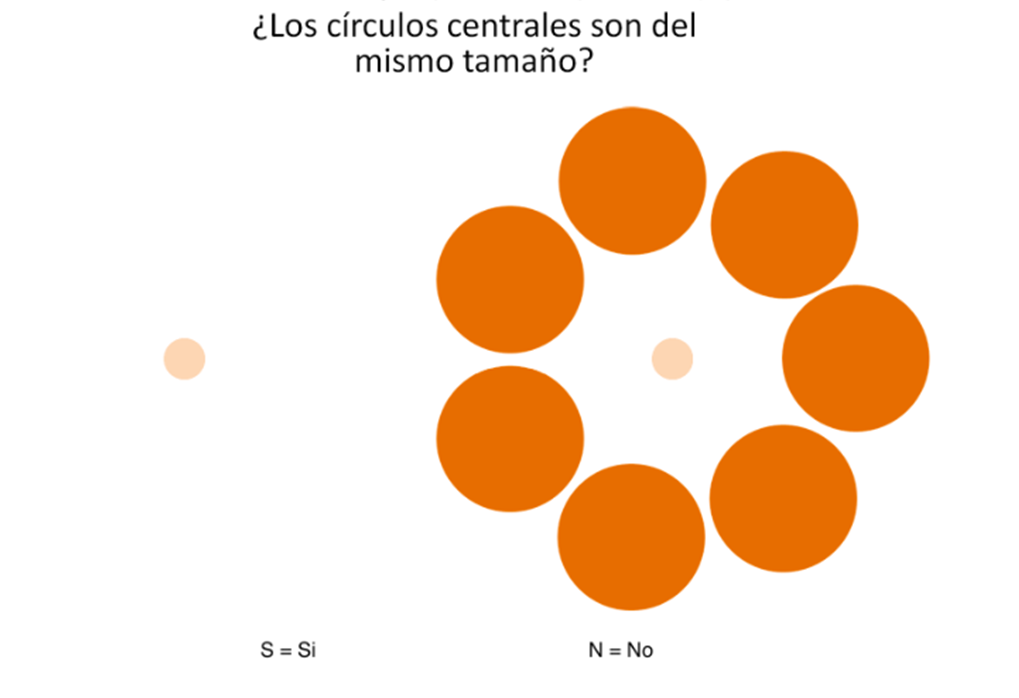
\includegraphics[width=0.60\textwidth]{Figures/Ejemplo_EnsayoYN_1}\\
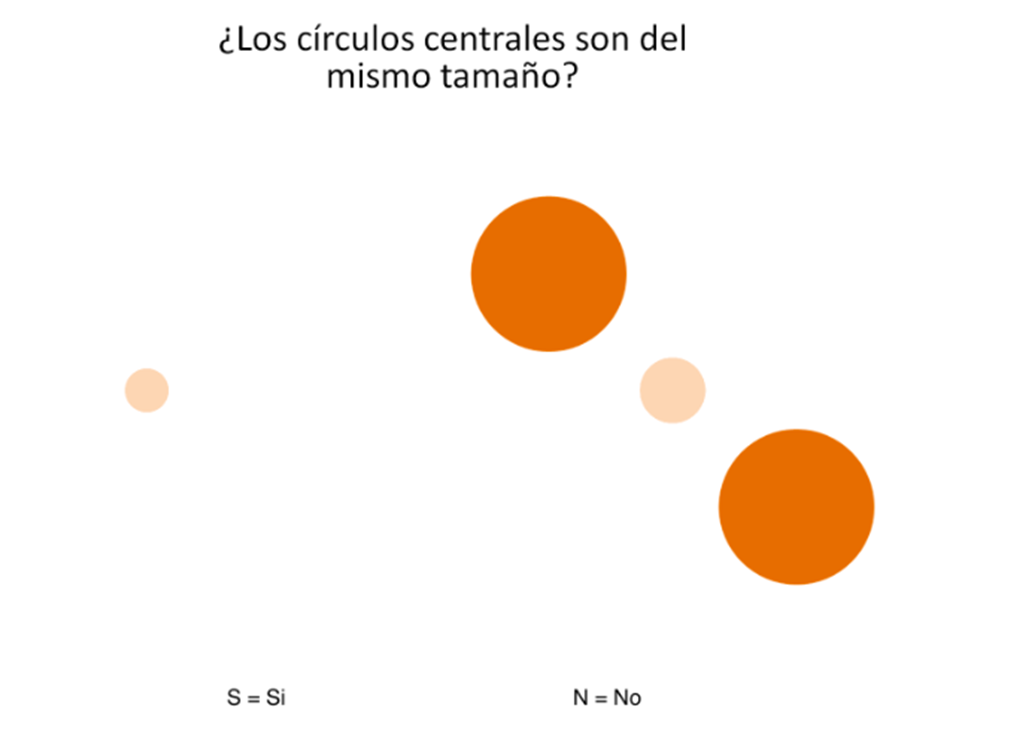
\includegraphics[width=0.60\textwidth]{Figures/Ejemplo_EnsayoYN_2}
%\decoRule
\caption[Presentación de ensayos con tarea de detección binaria]{Se muestra un par de capturas de pantalla ilustrativas de la tarea de detección binaria presentada a los participantes; en el panel superior, se presenta un ensayo de la clase A y en el panel inferior, la clase B.}
\label{fig:Ejem_YN}
\end{figure}

Los estímulos permanecían en pantalla durante 1.5 segundos con independencia de si los participantes habían, o no, emitido una respuesta: Si el participante respondía antes, los estímulos se quedaban en pantalla hasta cumplirse el intervalo, tras el cual se pasaba inmediatamente a la segunda fase del ensayo; si el participante no había respondido, los recordatorios permanecían solos en pantalla hasta que se registrara una respuesta. Esta restricción fue incluida para preveer la posibilidad de que los participantes se habituaran a la ilusión al prolongar su observación.\\

\item Fase 2: Escala de Confianza

%En una segunda fase, los participantes tuvieron que oprimir una tecla del 1 al 3 para indicar qué tan seguros estaban de la respuesta recién emitida.
Una vez registrada la respuesta de los participantes a la tarea Sí/No, se les mostró una segunda pantalla donde se les solicitaba que indicaran qué tan seguros se sentían de la respuesta binaria recién dada, de acuerdo con la escala presentada en pantalla, oprimiendo la tecla \textit{'1'}, \textit{'2'} ó \textit{'3'}, (ver Figura~\ref{fig:Ejem_Esc}). \\

Los puntajes registrados por los paricipantes -\textit{'1'},\textit{'2'} o \textit{'3'}- se tradujeron y registraron en una escala más grande -con valores del 1 al 6- que separa en direcciones opuestas la confianza que se tiene en los juicios de detección posibles, es decir, distingue entre la confianza que se tiene en que el estímulo evaluado contenga sólo ruido ('1 = Muy seguro de que NO son iguales'; \textit{'2'} =  \textit{'Más o menos seguro de que NO son iguales'}; \textit{'3'} = \textit{'Poco seguro de que NO son iguales'}) y la confianza de que se trate de un estímulo con señal (\textit{'4'} = \textit{'Poco seguro de que son iguales'}; \textit{'5'} = \textit{'Más o menos seguro de que son iguales'}; \textit{'6'} = \textit{'Muy seguro de que son iguales'}). La conversión de los puntajes emitidos a la escala de seis elementos se realizó en función a la respuesta binaria recién registrada, de la siguiente forma:

\begin{itemize}
\item En los ensayos en que el participante hubiera respondido \textit{'No'} a la pregunta de detección binaria \textit{'¿Los círculos centrales son del mismo tamaño?'}, la conversión de los puntajes de confianza asignados sería:\\
	\begin{itemize}
	\item 3 siendo \textit{'Estoy muy seguro de mi respuesta'}, se traduciría en \textit{'1'}.\\
	\item 2 siendo \textit{'Estoy más o menos seguro de mi respuesta'}, habría conservado el valor \textit{'2'}.\\
	\item 1 siendo \textot{'Estoy poco seguro de mi respuesta'}, se convertiría en \textit{'3'}.\\
	\end{itemize}
\\
\item En los ensayos donde el participante hubiera respondido \textit{'Sí'} en la primera fase, la transformación de los puntajes asignados habría sido la siguiente:\\
	\begin{itemize}
	\item 1 siendo \textit{'Estoy poco seguro de mi respuesta'}, se transformaría en \textit{'4'}.\\
	\item 2 siendo \textit{'Estoy más o menos seguro de mi respuesta'}, se registraría como \textit{'5'}.\\
	\item 3 siendo \textit{'Estoy muy seguro de mi respuesta'}, se convertiría en \textit{'6'}.\\
	\end{itemize}
\end{itemize}\\

De tal forma que los valores extremos de la escala construida representan una mayor seguridad en las respuestas emitidas en la fase anterior -\textit{'Sí'} o \textit{'No'}- y los valores intermedios, una mayor incertidumbre.\\

Esta forma de obtener la escala de confianza a partir de la yuxtaposición entre las respuestas de los participantes a la tarea binaria y la valoración de su confianza en las mismas, corresponde con el método utilizado en los Experimentos 1 y 2 de una serie de Experimentos donde se reporta evidencia del Efecto Espejo  en Memoria de Reconocimiento \parencite{Glanzer1990}, con el fin de facilitar la tarea de los participantes, evitar su fatiga y garantizar la coherencia entre las respuestas obtenidas en la tarea de bisección y el puntaje asignado en la escala de confianza.\\

\begin{figure}[th]
\centering
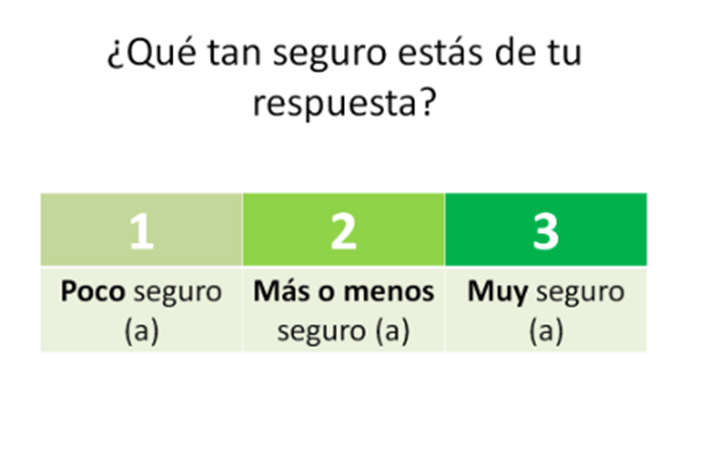
\includegraphics[width=0.65\textwidth]{Figures/Ejemplo_Escala}
%\decoRule
\caption[Presentación de la escala de confianza]{La escala de confianza mostrada a los participantes en la segunda fase de la tarea y  a partir de la cual se les solicitaba evaluar e indicar qué tan seguros se sentían del juicio de detección emitido con su respuesta inmediatamente anterior}
\label{fig:Ejem_Esc}
\end{figure}\\

Una vez registrada la segunda respuesta del participante -el puntaje asignado en la escala de confianza- se daba por terminado el ensayo.\\

\end{itemize}

%Entre cada ensayo, se presentó una pantalla intermedia que solicitaba a los participantes presionar la barra espaciadora para indicar que estaban listos para responder al siguiente ensayo.
Entre cada ensayo se incluyó una pantalla \textit{'de descanso'} que indicaba a los participanes que debían presionar la barra espaciadora para continuar. Estas pantallas \textit{pausa} otorgaban control a los participantes de su avance en el experimento y fueron incluídas para garantizar que estuvieran prestando atención durante la presentación -restringida en el tiempo- de los estímulos a comparar.\\

Al terminar los 640 ensayos, se mostraba una última pantalla donde se presentaba la retroalimentación general del desempeño de cada participante (Total de aciertos y errores cometidos), únicamente con el fin de marcar el \textit{'cierre'} de su participación. En ningún momento se informó a los participantes sobre el propósito de la investigación, ni sobre la existencia de los niveles de dificultad entre los cuales se compararía su ejecución.\\ 

%Se registraron tiempos de respuesta por cada respuesta registrada (Respuesta en la tarea Sí/No; Respuesta en la escala de confianza) y  la duración del experimento completo.
Además de las respuestas dadas por los participantes, se registraron también los tiempos de respuesta a lo largo del experimento (latencias). En el Apéndice \ref{App_Registro} se muestra y desarrolla en detalle cuáles fueron los datos obtenidos y registrados por cada uno de los participantes.\\

\begin{figure}[th]
\centering
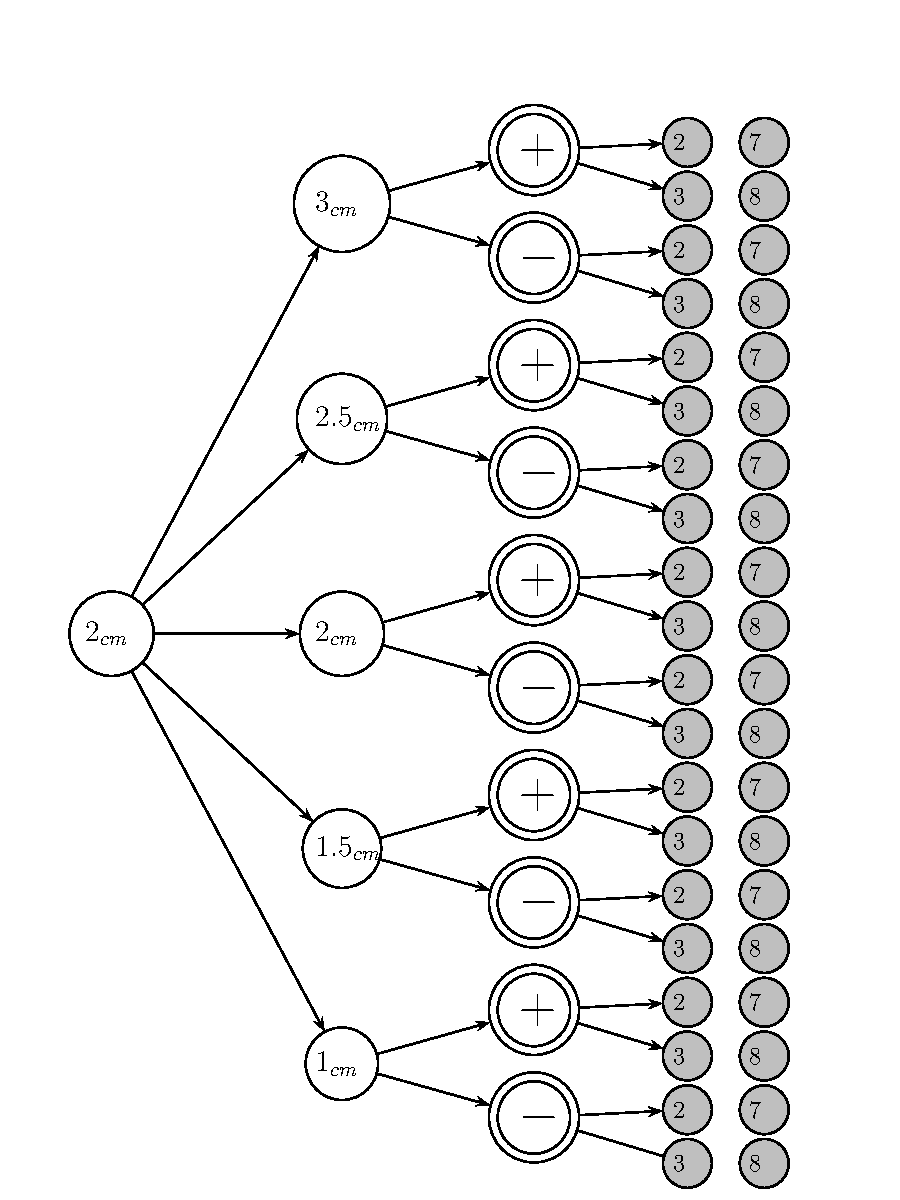
\includegraphics[width=0.9\textwidth]{Figures/Estimulos_Experimento1} 
\decoRule
\caption[Diseño de Estímulos en el Experimento 1]{Diseño factorial 5x2x2 utilizado para construir las figuras de Ebbinghaus presentadas en el Experimento 1, cuyo círculo central debía compararse con un círculo de referencia de $2cm$ de diámetro, (en el lado izquierdo de la figura). El tamaño central del círculo de la figura de Ebbinghaus se presentó en cinco tamaños diferentes, con círculos externos que inducieran efectos de sobrestimación (+) o subestimación (-) y con dos variaciones del \textit{'número de círculos externos'} por clase (2 y 3 círculos externos en la clase A, o 7 y 8 en la clase B). En total, cada clase quedó conformada por 16 estímulos Ruido, (presentados 10 veces en cinco colores diferentes) y cuatro Señales (presentados 40 veces, en cinco colores diferentes), es decir, 320 ensayos por clase y 640 en todo el experimento.}
\label{fig:Exp_1}
\end{figure}

\begin{figure}[th]
\centering
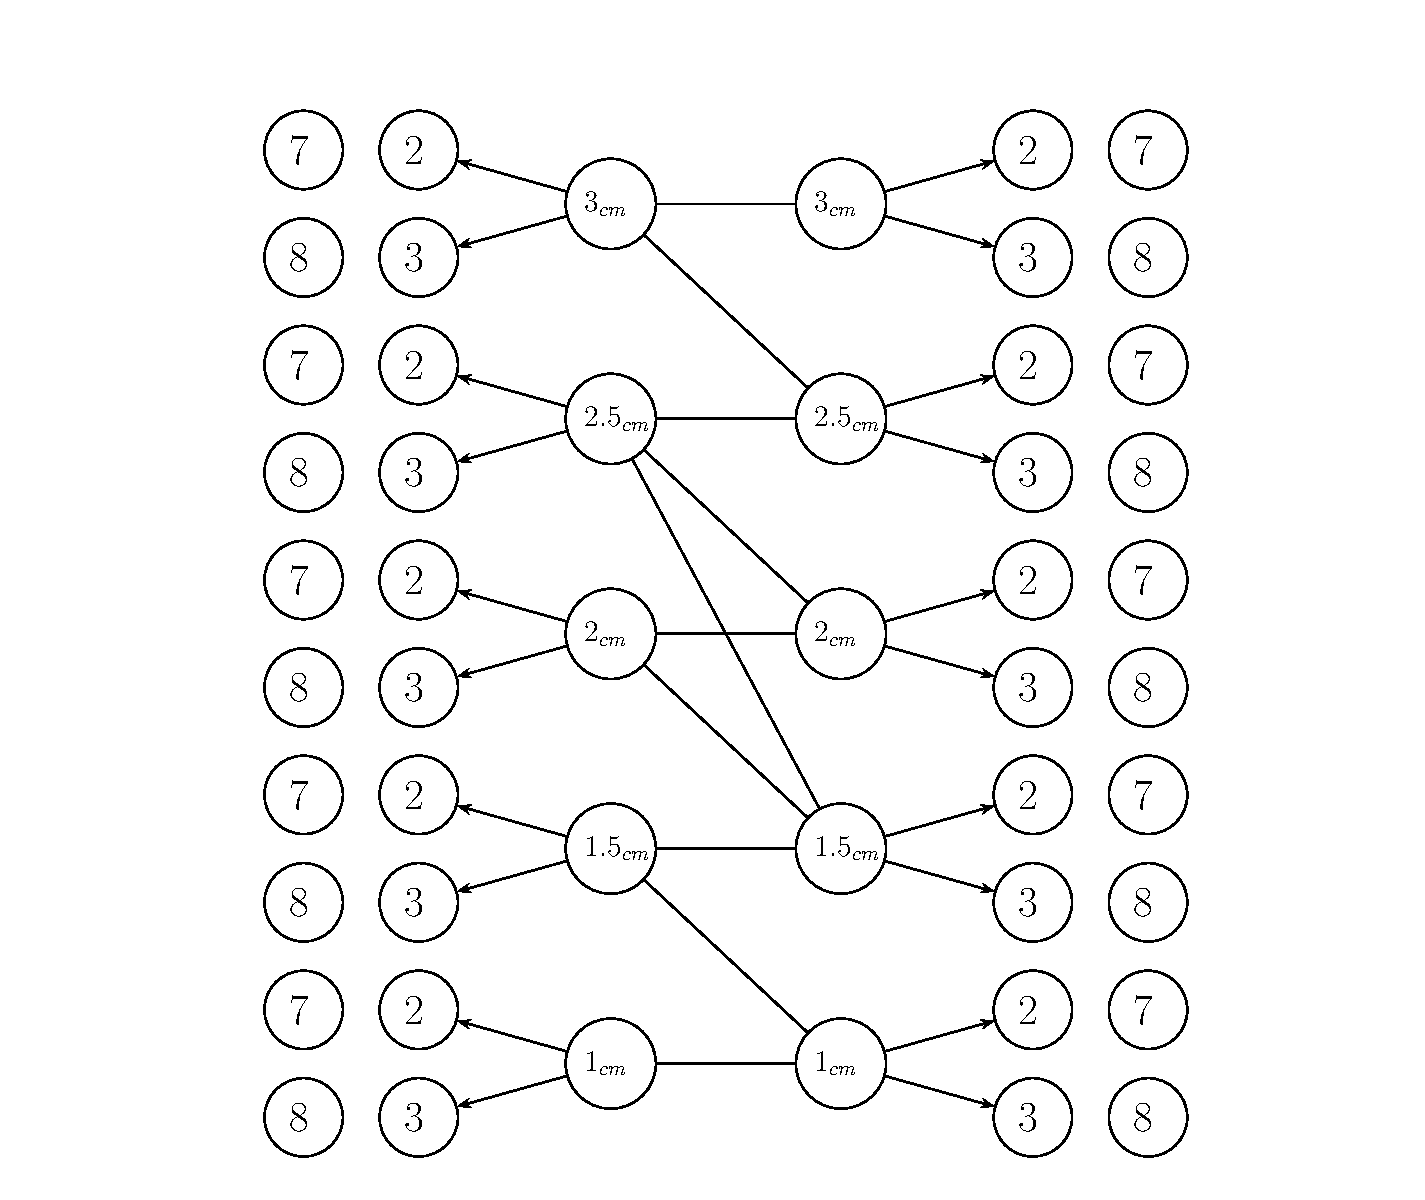
\includegraphics[width=0.95\textwidth]{Figures/Estimulos_Experimento2} 
\decoRule
\caption[Diseño de Estímulos en el Experimento 2]{Diseño de las parejas de figuras de Ebbinghaus mostradas en el Experimento 2, compuestas por una figura con efecto de subestimación y una con efecto de sobrestimación. Con los cinco tamaños distintos de círculo central propuestos se crearon cinco parejas iguales (señales) y cinco parejas arbitrarias desiguales (ruido). Por cada una de las diez parejas se consideró las cuatro combinaciones posibles entre los niveles de círculos externos incluídos en cada condición - 2 vs 2 o 7 vs 7; 3 vs 3 u 8 vs 8; 2 vs 3 o 7 vs 8; 3 vs 2 o 8 vs 7) Cada pareja se repitió ocho veces, contrabalanceando la posición derecha-izquierda de los efectos de sobrestimación y subestimación.}
\label{fig:Exp_2}
\end{figure}
\end{itemize}


 
% Chapter 1

\chapter{Resultados} % Main chapter title
\label{Cap_Res} % For referencing the chapter elsewhere, use \ref{Chapter1} 

\section{Datos recolectados}

%SDatos duros antes del análisis.
Antes de realizar análisis estadísticos para determinar si se encontró -o no- evidencia sólida del Efecto Espejo en nuestros experimentos, los datos recopilados se exploraron de manera exhaustiva, graficando la relación entre la ejecución de los participantes y diferentes variables.\\ 

%Se destaca la implrtancia de revisar los datos antes de someterlos a analisis estadísticos
Graficar los datos antes de someterlos al análisis estadístico, constituye una práctica recomendable en tanto que 1) permite evaluar la pertinencia del diseño experimental a la luz de las respuestas registradas y 2) proporciona un filtro para comprobar que los participantes estuvieran respondiendo de manera congruente y consistente con las tareas presentadas, permitiendo una mayor confianza en las conclusiones que resulten de su análisis.\\

%Presentación de los controles graficados: Atención, El efecto del paso del tiempo y las variables externas en los estímulos. 
A continuación se presentan las distintas gráficas realizadas para explorar tres grandes fuentes de ruido que potencialmente podrían haber influido en el desempeño de los participantes (contaminando los datos obtenidos). Dichas fuentes son:\\

\begin{enumerate}
	\item \textbf{¿Las respuestas se emiten en trenes?} (\textit{Evaluando la atención}).\\

Para evaluar que los participantes estuvieran poniendo atención a las tareas presentadas, se revisaron las respuestas emitidas a lo largo de los ensayos.\\

Durante los experimentos los estímulos con Ruido o Señal de las clases de estímulos diseñadas eran presentados de manera aleatoria, por lo que se esperaría encontrar mucha variabilidad en las respuestas emitidas por los participantes (y que usaran todas las opciones de respuesta). En caso contrario, la persistencia en la emisión de una misma respuesta de manera consecutiva (\textit{trenes de respuesta}), podría sugerir una falta de atención a los etímulos en pantalla y una posible dependencia entre respuestas.\\

	\item \textbf{¿El Aprendizaje o la Fatiga alteran la ejecución de los participantes?}  (\textit{Evaluando cambios en el desempeño a lo largo del tiempo}).\\

Un segundo filtro consistió en la evaluación de los posibles efectos que el paso del tiempo (y el avance entre ensayos) pudo haber tenido sobre el desempeño de los participantes. Por un lado, dado que los experimentos estuvieron compuestos por un amplio número de ensayos -cada uno con un par de tareas de detección-, la \textbf{Fatiga} es un riesgo latente. Por otro lado, dado que la tarea experimental consistió en la presentación de ilusiones ópticas, es posible que la exposición repetida a estas redujera su impacto por efecto de \textbf{Habituación}, mejorando el desempeño de los participantes.\\

	\item \textbf{¿Los participantes tienen alguna preferencia hacia la emisión de ciertas respuestas ante cierto tipo de estímulos?} (\textit{Evaluando el efecto de las variables manipuladas en la construcción de los estímulos}).\\

Finalmente, se evaluó el impacto que las variables manipuladas para diseñar los estímulos pudieran haber tenido sobre 1) la intensidad de la ilusión óptica y 2) la emisión de respuestas de los participantes.\\
\end{enumerate}

Idealmente, el desempeño de los participantes no debería cambiar en función a ninguna de las fuentes de ruido presentadas, y sólo presentar diferir significativamente entre las clases A y B diseñadas.\\












\subsection{Control 1: ¿Los participantes estaban poniendo atención a la tarea al emitir sus respuestas?}

Los experimentos realizados estuvieron compuestos de 640 ensayos, a lo largo de los cuales los participantes tuvieron que 1) decidir si los estímulos presentados cumplían con la condición que se les solicitó detectar y 2) valorar su certidumbre sobre esta primer respuesta y asignarle un puntaje. Dado lo demandante y extenso del procedimiento, la primer preocupación respecto de la validez de los datos obtenidos fue determinar si los participantes habían -o no- respondido a la tarea con atención. Para ello, se revisaron las respuestas emitidas ensayo a ensayo para garantizar todas las opciones de respuesta se hubieran usado y que la variabilidad en la emisión de respuestas correspondiera con la naturaleza aleatoria con que se presentaban los distintos tipos de estímulo.\\

\begin{itemize}
	\item Emisión de respuestas 'Sí/No' a lo largo del experimento.

Primero se graficaron las respuestas emitidas durante la tarea de detección binaria ('Sí, los círculos son iguales' o 'No, los círculos son diferentes'), ensayo a ensayo. Con estos gráficos se buscó descartar la presentación de trenes de respuesta lo suficientemente largos como para sugerir, dada la aleatoriedad con que los estímulos fueron presentados por el programa, una preferencia en el participante a responder a una tecla en particular, con independencia del estímulo a evaluar en pantalla.\\

%Participante representativo: Respuestas 'No' por 80 ensayos
La Figura~\ref{fig:Resp_E2_P1} presenta un ejemplo particularmente ilustrativo de la importancia que tiene revisar los datos antes de realizar el análisis estadístico. El gráfico muestra las respuestas emitidas en la tarea de detección binaria por el Participante 1 del Experimento 2, quien pasó los primeros 80 ensayos del experimento presionando persistentemente la tecla de respuesta 'No'. Este tren de respuesta fue considerado lo suficientemente largo como para cuestionar la atención con que el Participante 1 estuvo respondiendo a la tarea.\\ 

\begin{figure}[th]
\centering
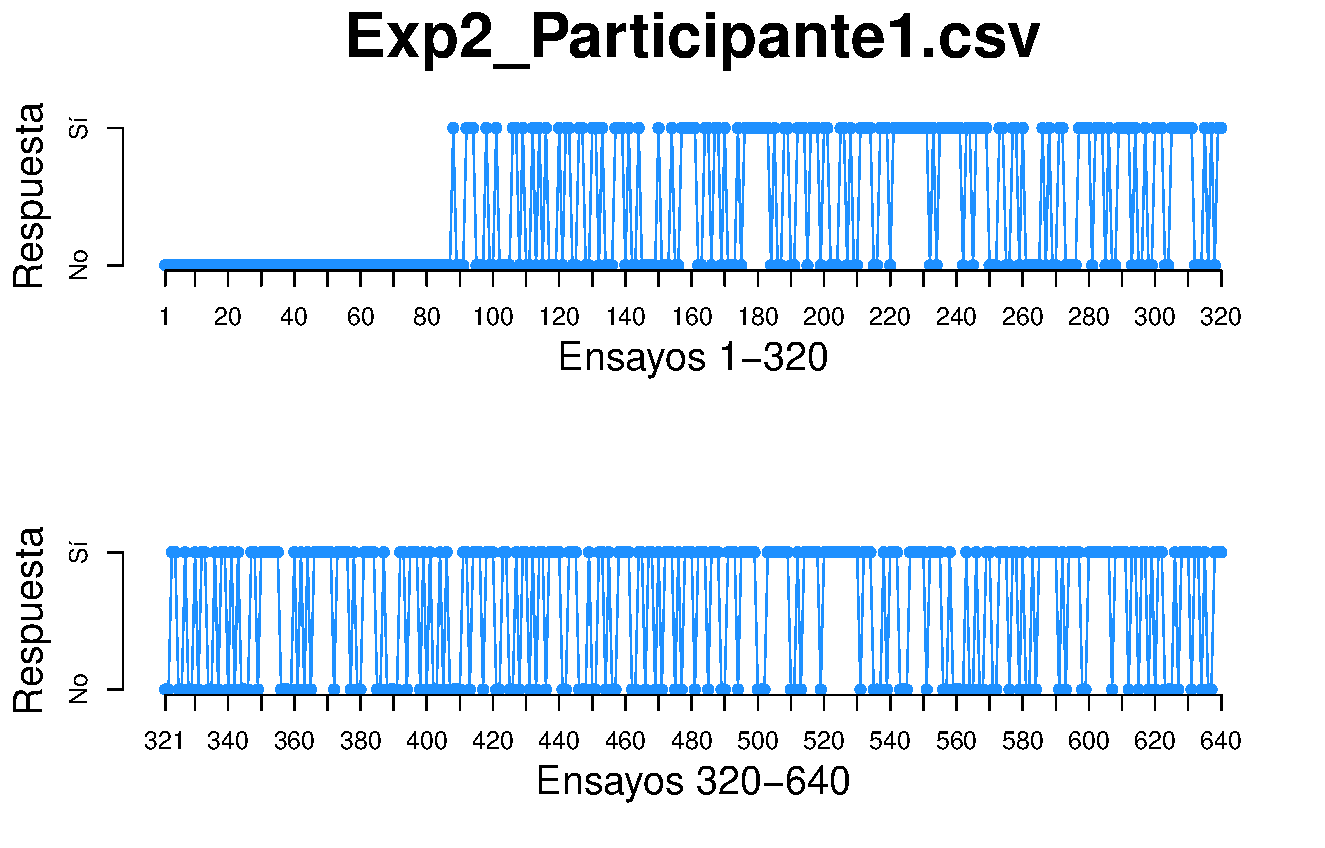
\includegraphics[width=0.80\textwidth]{Figures/Response_Exp2_P1} 
%\decoRule
\caption[Respuesta emitida por ensayo: Ejemplo de participante sesgado]{Respuestas Sí/No emitidas en los 640 ensayos del Experimento 1 por el Participante 1. En la gráfica se aprecia un tren de respuesta, que se extiende a lo largo de 80 ensayos, donde el Participante 1 sólo utilizó una de las opciones de respuesta disponibles.}
\label{fig:Resp_E2_P1}
\end{figure}

%Las gráficas correspondientes al resto de los participantes en los Experimentos 1 y 2, se muestran en las Figuras~\ref{fig:Response_P1} y \ref{fig:Response_E2}, respectivamente.\\

	\item Correlación entre las respuestas 'Sí/No' emitidas y el tipo de estímulo presentado en cada ensayo.

Como paso siguiente, se añadieron indicadores que señalaran las características de los estímulos presentados en cada ensayo -es decir, si se trataba de una Señal o Ruido, o si se trataba de un estímulo de la clase Fácil o Difícil-.\\ 

Retomando el caso del Participante 1 del Experimento 2 presentado en la Figura~\ref{fig:Resp_E2_P1}, la Figura~\ref{fig:BiasResp_E1_P1} permite evaluar la posibilidad de que las respuestas registradas estuvieran relacionadas con los estímulos presentados en pantalla, (por ejemplo, en el improbable -pero posible- caso de que se le hubiera presentado una gran proporción de estímulos con Ruido durante los primeros 80 ensayos del experimento). De acuerdo con esta gráfica, parece ser que el tren de 80 respuestas 'No' consecutivas se mantuvo con independencia del tipo de estímulo presentado. Con base en ello, se decidió eliminar a dicho participante de la muestra a analizar, al encontrarse evidencia suficiente para cuestionar la atención con que respondió a la tarea.\\

\begin{figure}[th]
\centering
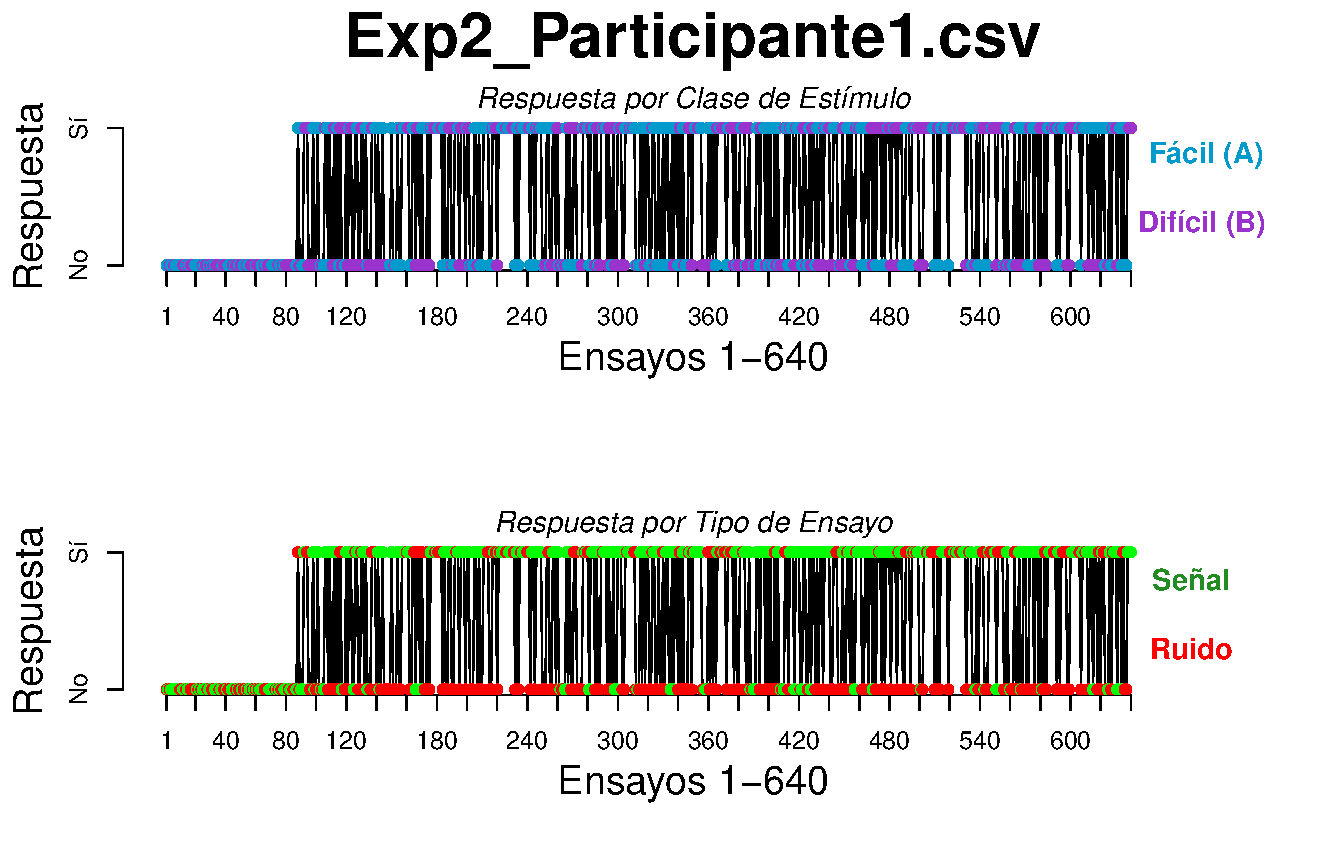
\includegraphics[width=0.80\textwidth]{Figures/BiasResp_Exp2_P1} 
%\decoRule
\caption[Respuesta por Tipo de Estímulo; ejemplo de participante sesgado]{Respuestas registradas por el Participante 1 en cada uno de los 640 ensayos del Experimento 2, indicando con diferentes colores el tipo de estímulo que se le mostraba en cada ocasión. En el panel superior se señala con colores violeta y azul si el estímulo presentado pertenecía a la clase Difícil o Fácil, respectivamente, y en el panel inferior, si se trataba de una Señal o Ruido con los colores verde y rojo, respectivamente.}
\label{fig:BiasResp_E1_P1}
\end{figure}

%Las Figuras~\ref{fig:BiasResp_E1} y () muestran las gráficas correspondientes al resto de los participantes en el Experimento 1 y 2, respectivamente.\\

	\item Asignación de puntajes de confianza, (\textit{'1'},\textit{'2'} ó \textit{'3'}).

En la segunda fase del problema de detección presentado en cada ensayo, los participantes tenían que elegir entre tres opciones de respuesta (teclas 1, 2 y 3) para señalar \textit{cuánta} confianza tenían sobre la respuesta recién emitida (\textit{'poco seguro'}, \textit{'más o menos seguro'} o \textit{'muy seguro'}, respectivamente). Las respuestas fueron registradas por el programa como parte de una Escala mayor (con valores del 1 al 6), que permite diferenciar entre la confianza de haber rechazado correctamente un estímulo con Ruido (e.g. \textit{'1, estoy muy seguro de que los círculos eran diferentes'}) y la confianza de haber identificado correctamente un estímulo con Señal (e.g \textit{'6, estoy muy seguro de que los círculos son iguales'}), asignando los valores intermedios (\textit{3} y \textit{4}) a los puntajes asignados para señalar una confianza baja en la respuesta emitida (e.g. \textit{'3, poco seguro de que los círculos eran diferentes'} y \textit{'4, poco seguro de que los círculos eran iguales'}).\\

Tal y como se hizo con la tarea de detección binaria, se graficaron los puntajes de confianza registrados por los participantes en cada uno de los 640 ensayos que conformaron cada experimento. A manera de ejemplo, la Figura~\ref{fig:Rating_E2_P4} muestra los puntajes emitidos por el Participante 15 del Experimento 2 a lo largo de la tarea. Este participante, de acuerdo con lo que se esperaría encontrar, hizo uso de las tres teclas de respuesta, registradas de acuerdo a su correspondencia con la respuesta dada a la tarea binaria.\\ 
 
\begin{figure}[th]
\centering
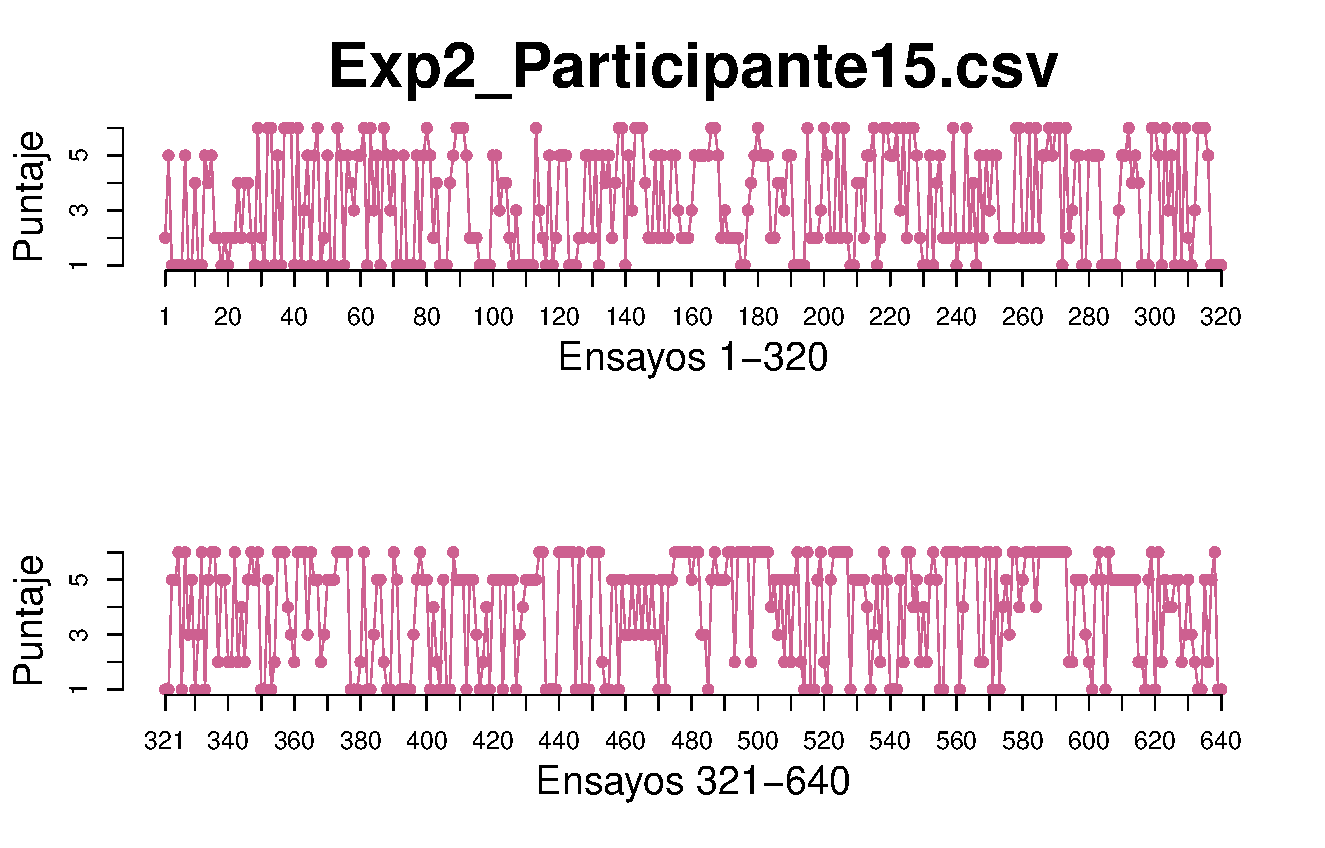
\includegraphics[width=0.80\textwidth]{Figures/Rating_Exp2_P15} 
%\decoRule
\caption[Asignación Puntaje de confianza: Ejemplo]{Puntajes de confianza asignados por el Participante 15 del Experimento 2 a las respuestas emitidas en la tarea binaria en cada uno de los 640 ensayos. El panel superior se muestran los puntajes asignados en los primeros 320 ensayos del experimento; en el panel inferior, los 320 restantes.}
\label{fig:Rating_E2_P4}
\end{figure}

%El registro ensayo a ensayo de los puntajes de confianza asignados por el resto de los participantes en los Experimentos 1 y 2 se muestran en las Figuras~\ref{fig:Rating_E1} y \ref{fig:Rating_E2}, respectivamente.\\

\end{itemize}










\subsection{Control 2: ¿La duración del experimento tuvo un impacto en la ejecución de los participantes?}

La fatiga causada por la extensión del experimento y la posible habituación a la ilusión óptica, fueron dos de las fuentes de ruido externo que se pensó podrían tener un efecto sobre la ejecución de los participantes, mermando la validez de los datos obtenidos. Para preveer su influencia, se incluyeron un par de controles desde el diseño experimental, tales como el agregar una pantalla de espera entre los ensayos que diera oportunidad a los participntes de descansar e indicar cuando se sintieran listos para atender un nuevo par de estímulos, o el restringir el tiempo durante el que se mostraban los estímulos a comparar. El siguiente conjunto de gráficas fueron realizadas para comprobar que ni la Fatiga ni la Habituación hubieran contaminado la ejecuciónde los participantes, esperando que su desempeño no mostrara signos de decaimiento o mejora con el paso de los ensayos.\\ 

\begin{itemize}
	\item Aciertos y errores a lo largo del tiempo

Primero, se graficó la clasificación de las respuestas emitidas por los participantes como acierto o error, en cada ensayo. Con ello se buscó explorar visualmente si hubieron cambios significativos en el desempeño de los participantes conforme adquirían más experiencia en la tarea.\\

La Figura~\ref{fig:Success_E2_P14} muestra como ejemplo el desempeño del Participante 14 durante el Experimento 2. La gráfica superior presenta el registro acumulativo de los aciertos y errores cometidos a lo largo de todo el experimento y en los paneles inferiores se muestra -ensayo a ensayo- si sus respuestas fueron registradas como acierto o error.\\

\begin{figure}[th]
\centering
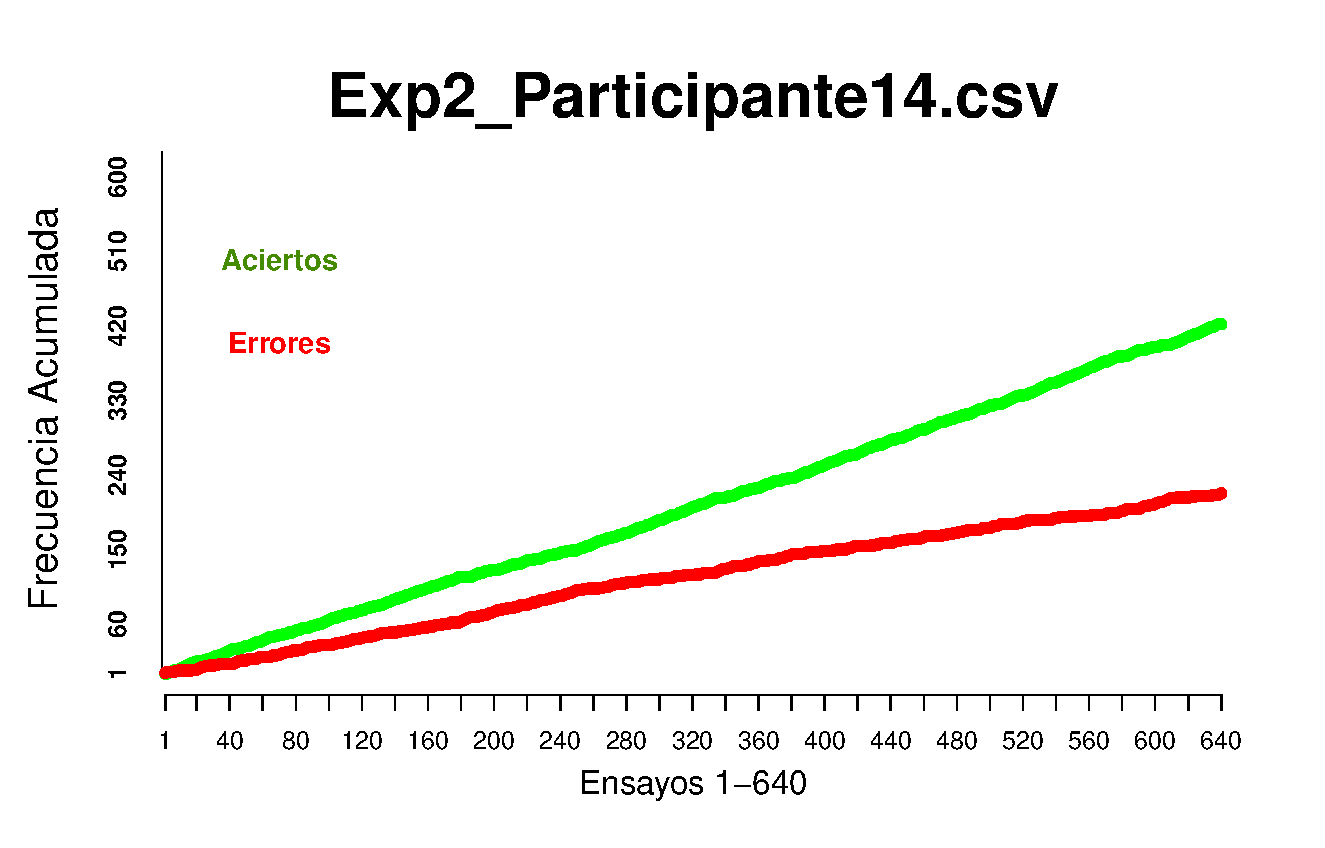
\includegraphics[width=0.60\textwidth]{Figures/SuccessCumulative_Exp2_P14} \\
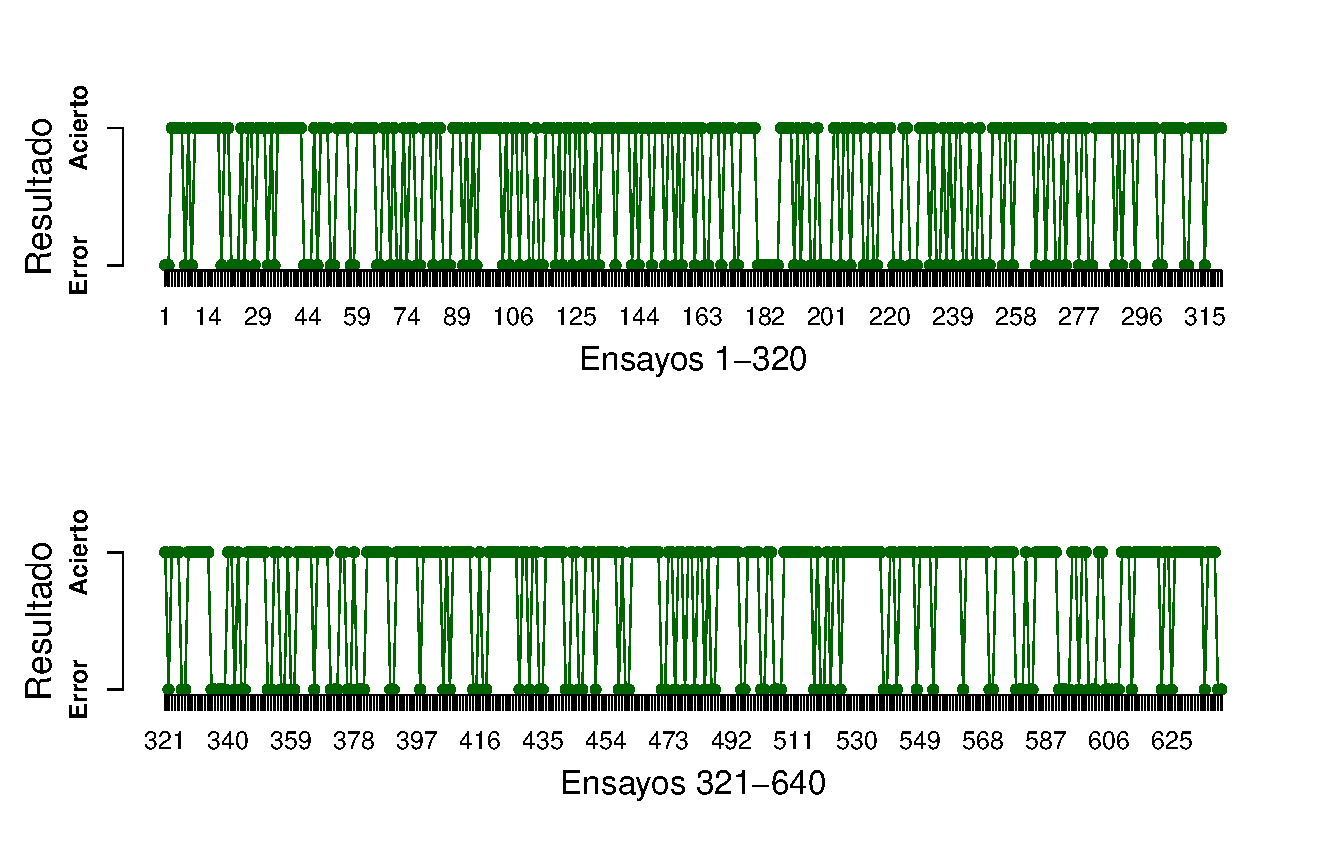
\includegraphics[width=0.80\textwidth]{Figures/Success_Exp2_P14}
%\decoRule
\caption[Aciertos y errores a lo largo del tiempo: Participante ejemplar]{Aciertos y errores cometidos por el Participante 14 del Experimento 2 a lo largo de la tarea. En el panel superior se muestra el registro acumulativo de estos a lo largo del experimento. Los paneles inferiores muestran la clasificación ensayo a ensayo de las respuestas emitidas por el participante como Acierto o Error (el panel intermedio presenta la primera mitad del experimento y el panel inferior, el resto).}
\label{fig:Success_E2_P14}
\end{figure}

%Las Figuras~\ref{fig:Success_E1} y \ref{fig:Success_E2} muestran los aciertos y errores cometidos a lo largo de los experimentos por el resto de los participantes en los Experimentos 1 y 2, respectivamente.\\


	\item Tipos de acierto y error a lo largo del tiempo

Para tener más información sobre los aciertos y errores cometidos, se realizaron gráficas que señalaran qué resultado habían obtenido los participantes en cada ensayo (Hit, Falsa Alarma, Rechazo y Omisión). En la Figura~\ref{fig:Outcome_E2_P14} se vuelven a presentar los datos del Participante 14 del Experimento 2, señalando el tipo de resultado obtenido. El panel superior muestra el registro acumulativo de cada uno de los cuatro posibles resultados a lo largo del experimento y el panel inferior, los resultados obtenido en cada ensayo.\\ 

\begin{figure}[th]
\centering
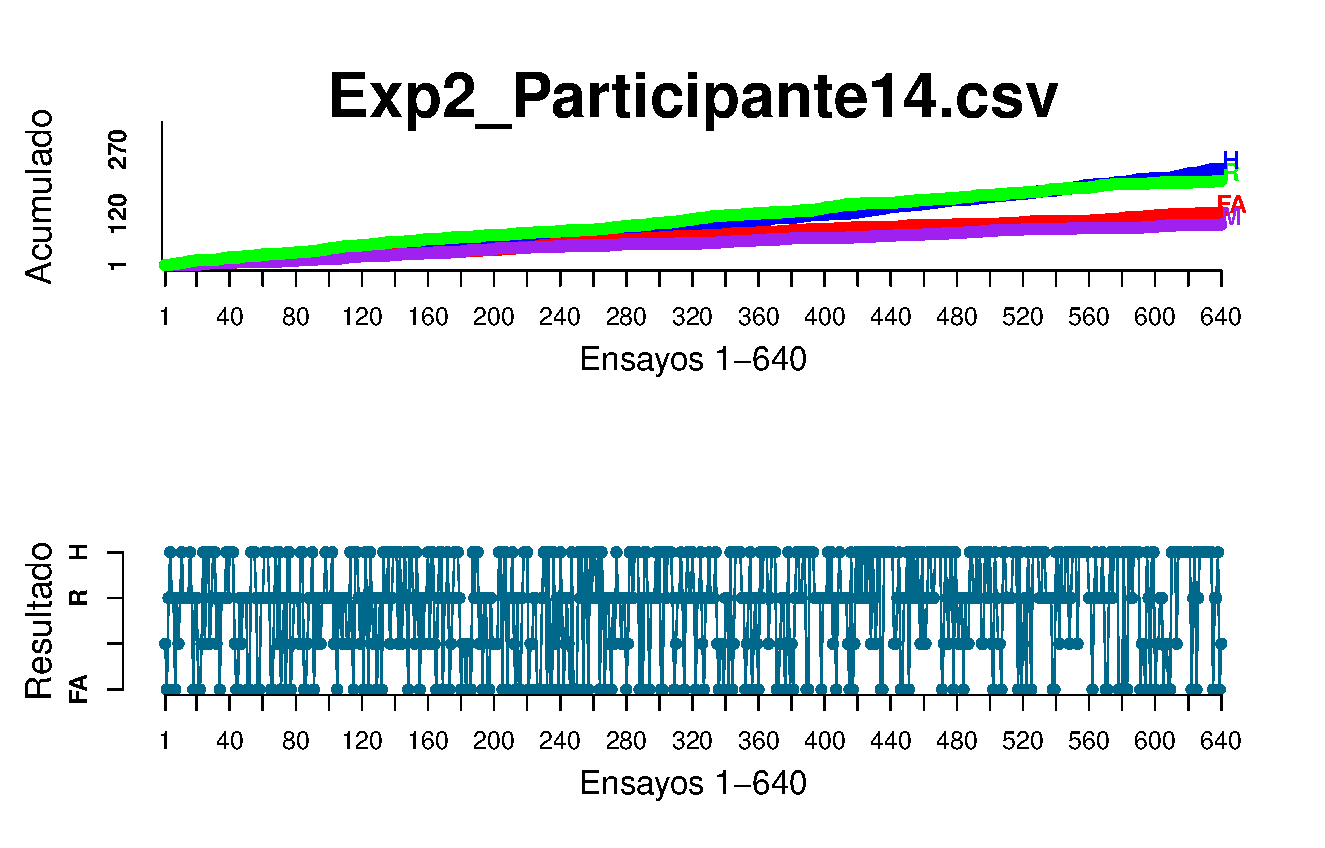
\includegraphics[width=0.80\textwidth]{Figures/Outcome_Exp2_P14}
%\decoRule
\caption[Resultado obtenido a lo largo del tiempo: Ejemplo]{Resultados obtenidos por el Participante 14 del Experimento 2 a lo largo del Experimento. En el panel superior se muestra la frecuencia acumulada de los Hits, Falsas Alarmas, Rechazos y Omisiones obtenidos durante el experimento, mientras que en el panel inferior se presenta el resultado obtenido por cada ensayo.}
\label{fig:Outcome_E2_P14}
\end{figure}


\end{itemize}










\subsection{Control 3: ¿El diseño de los estímulos afectó el desempeño de los participantes?}

Durante la construcción de los estímulos a presentar en los experimentos se manipularon dos variables: 1) El número de círculos externos incluidos en las figuras de Ebbinghaus y 2) el color en que se presentaron las figuras. La primera constituye la variable experimental, y con ella que se buscó definir las dos clases de estímulos entre las que se compararía el desempeño de los participantes. Por otro lado, las variaciones en la segunda variable mencionada fueron incluidas arbitrariamente, en un intento por hacer la tarea menos tediosa y más dinámica, buscando preveer los efectos de fatiga y habituación. Es decir, se esperaba que el desempeño de los participantes variara exclusivamente en función a los cambios en la variable experimental.\\

A continuación se presenta un último conjunto de gráficos, realizados para descartar la posibilidad de que el desempeño de los participantes se hubiera visto influido por el color en que los estímulos fueron presentados.\\

\begin{itemize}
	\item El efecto del color sobre la intensidad de la ilusión.

Una primer forma en que el color de las figuras pudo haber afectado el desempeño de los participantes fue alterando la intensidad de la ilusión de Ebbinghaus. Para evaluar dicha posibilidad, se exploró la posible relación entre el número total de Hits y Falsas Alarmas cometidos y los colores en que aparecían las figuras.\\

\begin{figure}[th]
\centering
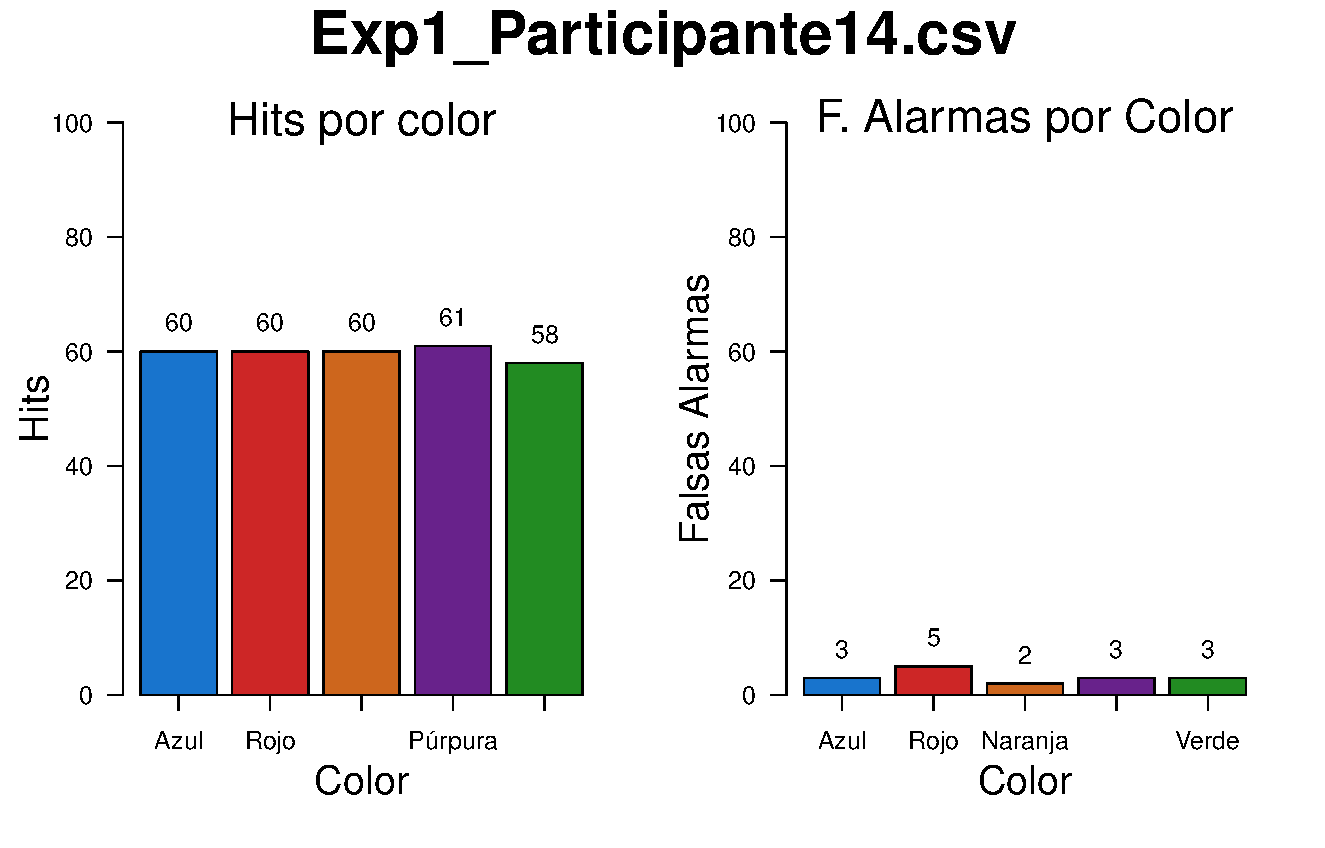
\includegraphics[width=0.85\textwidth]{Figures/Color_Exp1_P14}
%\decoRule
\caption[Hits y Falsas Alarmas por Color; Ejemplo]{Número de Hits (panel izquierdo) y Falsas Alarmas (panel derecho) cometidas por el Participante 14 del Experimento 1 por cada uno de los colores en que se presentaron las figuras. Se omite el número de Omisiones y Rechazos Correctos obtenidos, al tratarse del complemento de las cifras presentadas.}
\label{fig:Color_E1_P14}
\end{figure}

Por ejemplo, la Figura~\ref{fig:Color_E1_P14} muestra la cantidad de Hits y Falsas Alarmas cometidas por el Participante 14 a lo largo del Experimento 1 por cada color empleado en el diseño de las figuras (panel izquierdo y derecho, respectivamente). De acuerdo a lo que se observa, no parece que el color haya tenido un efecto sobre la precisión con que este participante respondía a la tarea.\\


	\item El Efecto del Color sobre la emisión de respuestas en los participantes.

Una segunda forma en que el color de los estímulos pudo haber alterado el desempeño de los participantes, es si estos hubieran tenido un sesgo o preferencia a responder de cierta forma ante alguno de los colores utilizados con independencia del resto de las características de las figuras. Para explorar esta posibilidad, se graficó la relación entre el color de las figuras y la proporción de respuestas afirmativas y negativas emitidas por cada participante. La Figura~\ref{fig:BiasCol_E1_P13} presenta un ejemplo de este tipo de gráficas, donde se muestra la proporción de Respuestas Sí/No emitidas por el Participante 13 del Experimento 1 para cada uno de los diferentes colores en que se presentaron los estímulos. Como se puede ver en la figura, parece ser que este participante mantuvo constante la proporción de respuestas afirmativas y negativas emitidas a lo largo de los distintos colores utilizados, por lo que no parece que el color hubiera tenido un efecto sobre su propensión a responder de manera afirmativa o negativa.\\

\begin{figure}[th]
\centering
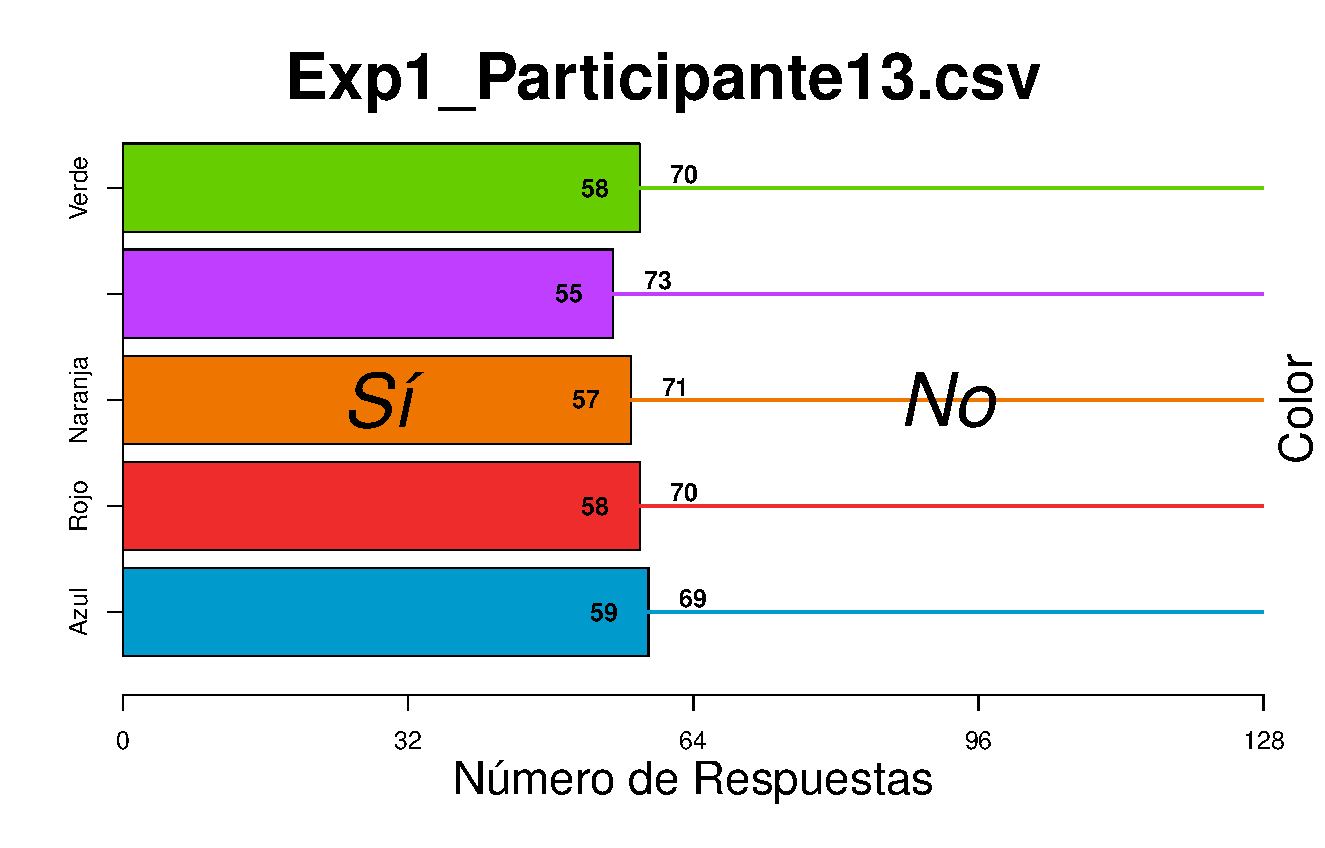
\includegraphics[width=0.80\textwidth]{Figures/BiasColor_Exp1_P13}
%\decoRule
\caption[Proporción de Respuestas Sí/No por color; Ejemplo]{Se muestra la proporción de respuestas afirmativas y negativas emitidas por el Participante 14 del Experimento 1 en función al color en que se presentaron los estímulos.}
\label{fig:BiasCol_E1_P13}
\end{figure}
\end{itemize}

%De cualqueir forma, se presentó siempre un mismo número de figuras por cada color, para cada uno de los estímulos construidos. Es decir, que aún cuando se hubiera encontrado evidencia de variaciones en el desempeño de los participantes en función de los colores utilizados, se esperaría que dicho efecto se distribuyera de manera homogénea entre las dos clases de estímulos entre las cuales se compararía su ejecución.\\

Las gráficas correspondientes al desempeño de cada uno de los participantes en los Experimentos 1 y 2, así como los códigos empleados para su graficación, se pueden consultar en línea en el siguiente repositorio de GitHub: \href{http://github.com/Adrifelcha/MirrorEffect-Adrifelcha}{http://github.com/Adrifelcha/MirrorEffect-Adrifelcha}.\\




































\section{Análisis estadísticos}

En los experimentos realizados, los patrones de respuesta identificados como parte del Efecto Espejo se presentaron en más de tres cuartas partes de los participantes, en al menos uno de los dos protocolos de detección empleados. De los veinte participantes en el Experimento 1, diecisiete ($85\%$) mostraron el patrón de respuesta esperado en la tarea binaria y dieciocho ($90\%$), en la Escala de Confianza. A su vez, en el Experimento 2, dieciocho de los veinte participantes incluidos en la muestra ($90\%$) presentaron los patrones del Efecto Espejo en ambas tareas. Estas proporciones resultan estadísticamente significativas al compararlas contra el azar con una prueba binomial simple (ver Tabla~\ref{Tabla_Binom}).\\

\begin{table}
\caption[Pruebas Binomiales que comparan la proporción de patrones de Efecto Espejo encontrados]{Se presentan los resultados de la comparación entre la proporción de casos con el Efecto Espejo encontrados en cada experimento y el azar ($p=0.5$), de acuerdo con la realización de pruebas binomiales.}
\label{Tabla_Binom}
\centering
\begin{tabular}{l l | c c c}
\toprule
%\tabhead{Groups} & \tabhead{Treatment X} & \tabhead{Treatment Y} \\
\textbf{} & \textbf{Tarea} & \textbf{Proporción} & \textbf{P value}\\
\midrule
Exp 1 & Sí/No & 17/20 & 0.0025 \\
Exp 1 & Escala & 18/20 & 0.0004\\
Exp 2 & Sì/No & 18/20 & 0.0004\\
Exp 2 & Escala & 18/20 & 0.0004\\
\bottomrule
\end{tabular}
\end{table}


Tomando en cuenta que las clases de estímulos a comparar se diseñaron de manera exploratoria y que la tarea de detección planteada se presentó en términos de dos protocolos distintos, el análisis de datos se llevó a cabo en el siguiente orden:\\

\begin{enumerate}
\item \textbf{Verificar que realmente existiera una diferencia entre las clases de estímulos construidas}\\

Dado que las clases de estímulos a comparar fueron construidas con base en la literatura revisada sobre el funcionamiento de la ilusión de Ebbinghaus, se comenzó por evaluar que realmente existienran distintos niveles distintos de discriminabilidad entre éstas y que dicha diferencia se presentara en la dirección esperada. Para ello, se compararon los valores de $d'$ calculados a partir de los subconjuntos de Hits y Falsas Alarmas obtenidos por cada clase, para corroborar que se satisfaciera la siguiente relación:\\

\begin{center}
 $d'(A) > d'(B)$\\
 donde A y B representan las clases de estímulos construidas en función del número de círculos externos contenidos en las figuras: la clase A con \textit{pocos} círculos (2 o 3 círculos) y la clase B con \textit{muchos} círculos (7 u 8).\\
\end{center}

\item \textbf{Comparar las tasas de Hits y Falsas Alarmas entre condiciones.}\\

Una vez corroborada la diferencia entre las clases de estímulos construidas, se evaluaron las diferencias encontradas entre las tasas de Hits y Falsas Alarmas registradas por cada clase de estímulo para comprobar que dicha discrepancia fuera significativa, cumpliendo con el siguiente patrón reportado en estudios de memoria de reconocimiento:\\

\begin{center}
$H(B) < H(A)$\\
$FA(A) < FA(B)$\\
donde $H$ y $FA$ representan las tasas de Hits y Falsas Alarmas obtenidas en cada clase de estímulos a evaluar. Es decir:\\
$FA(A) < FA(B) < H(B) < H(A)$\\
\end{center}

\item \textbf{Comparar el puntaje de confianza promedio asignado a cada tipo de ensayo (con ruido o señal) entre cada clase a comparar}\\

Dado que la clase A es más discriminable que B, esperaríamos que los participantes hubieran reportado un promedio mayor de confianza al responder a los estímulos de la clase A, ($PuntajeCrudo(A) > PuntajeCrudo(B)$). Pero tomando en cuenta que los experimentos fueron programados de manera que los puntajes crudos emitidos por los puntajes (del 1 al 3) fueran transformados en una escala más grande que distinguiera entre la confianza en sus respuestas afirmativas y negativas, la relación entre los promedios de los puntajes transformados debería mostrar el mismo patrón que se reporta en la literatura en memoria:

%Posteriormente, se compararon los puntajes de confianza asignados a cada tipo de ensayo (Señal o Ruido) por cada clase de estímulo (Fácil o Difícil).\\

%Primero, en función de los puntajes de confianza crudos asignados por los participantes -el registro de las teclas de respuesta 1, 2 y 3-, se esperaba encontrar la siguiente relación en función de los niveles de dificultad:

%\begin{center}
%$P(A) > P(B)$\\
%donde $P$ refiere al promedio de los puntajes de confianza asignados a las respuestas emitidas por los participantes durante la tarea binaria, por cada condición de dificultad.\\
%\end{center}

%Después, tomando en cuenta que los experimentos fueron programados de tal manera que los puntajes registrados por los participantes -para indicar qué tan seguros se sentían respecto de la respuesta emitida en ese mismo ensayo a la tarea de detección binomial- fueran \textit{transformados} a valores dentro de una Escala mayor que distingue entre la confianza en las respuestas negativas y la confianza en las respuestas afirmativas, se espera encontrar la misma relación reportada en Memoria de Reconocimiento entre los promedios de los puntajes de confianza asignados por cada tipo y clase de estímulos:\\

\begin{center}
$P(BS) < P(AS)$\\
$P(AN) < P(BN)$\\
donde nuevamente $P$ refiere al promedio de los puntajes de confianza asignados a cada tipo de ensayo por cada clase de estímulo. Es decir:\\
$P(AN) < P(BN) < P(BS) < P(AS)$\\
\end{center}

\item \textbf{Réplica de controles reportados en la literatura.}\\

Además de evaluar las diferencias encontradas en la ejecución de los participantes entre las clases de estímulos construidas, en la literatura del Efecto Espejo también suelen reportarse algunos análisis estadísticos de control para confirmar la solidez del efecto encontrado, (Glanzer y Adams, \citeyear{Glanzer1990}). En el presente trabajo se retomó la revisión de la posible correlación entre los tiempos de respuesta invertidos por los participantes y las clases de estímulos a comparar. De acuerdo con la literatura, descartar esta correlación es importante en tanto que permite descartar que los resultados encontrados sean producto de una diferencia en el tiempo invertido por parte de los participantes al responder a cada clase.\\
\end{enumerate}

Todos los análisis previamente descritos fueron realizados desde dos enfoques distintos:\\

\begin{itemize}
\item Como una réplica de los análisis reportados en la literatura. \textit{(ANOVA's y Pruebas T)}.\\

Tomando en cuenta que el objetivo princial del trabajo de investigación realizado fue evaluar la generalizabilidad de los patrones de respuesta identificados en memoria de reconocimiento como Efecto Espejo en una tarea de detección perceptual, se consideró necesario someter los datos obtenidos a los mismos análisis reportados en la literatura. Para ello, se utilizó como guía un artículo que reporta evidencia del Efecto Espejo en cinco experimentos de memoria de reconocimiento donde se manipulan distintas variables para la definición de las clases A y B, (Glanzer y Adams, \citeyear{Glanzer1990}).\\

\item El desarrollo de modelos Bayesianos para la estimación paramétrica y la evaluación de la evidencia encontrada.\\

La estadística bayesiana es una herramienta flexible para el análisis de datos, que permite formalizar y evaluar las hipótesis que se tiene sobre el funcionamiento de ciertos procesos psicológicos especificando una distribución prior y una función de verosimilitud que describa la relación entre los datos obtenidos y los modelos estadísticos-cognitivos que dan cuenta de los fenómenos psicológicos que subyacen a su generación, (Lee, \citeyear{Lee2011}). En la presente Tesis, además de realizar los análisis estadísticos frecuentistas comúnmente reportados en los estudios en memoria de reconocimiento, se incluyeron desarrollaron modelos y análisis bayesianos para evaluar con mayor detalle la variabilidad contenida en las respuestas emitidas por los participantes.\\
\end{itemize}










\subsection{Evaluación de las diferencias entre las clases de estímulos propuestas}

En los experimentos realizados como parte de la presente tesis, las clases A y B fueron definidas de acuerdo con la literatura que ha explorado el impacto que tienen los distintos elementos que componen las figuras de Ebbinghaus en la intensidad de la ilusión evocada, (Massaro y Anderson, \citeyear{Massaro1971}), de la siguiente forma: \\

\begin{itemize}
\item \underline{Clase A}, (\textit{Fácil}): Figuras de Ebbinghaus compuestas por 2 o 3 círculos externos.\\

\item \underline{Clase B}, (\textit{Difícil}): Figuras de Ebbinghaus con 7 u 8 círculos externos.\\
\end{itemize}

Para evaluar la eficacia del diseño de las clases de estímulos propuestas, comprobando que estas realmente difirieron en términos de qué tan difícil resultó para los participantes discriminar entre los estímulos con Señal y aquellos con Ruido, se compararon los valores de $d'$ estimados para cada una de ellas, de acuerdo con el registro de Hits y Falsas Alarmas obtenidos por todos los participantes en los experimentos realizados.\\

\begin{figure}[th]
\centering
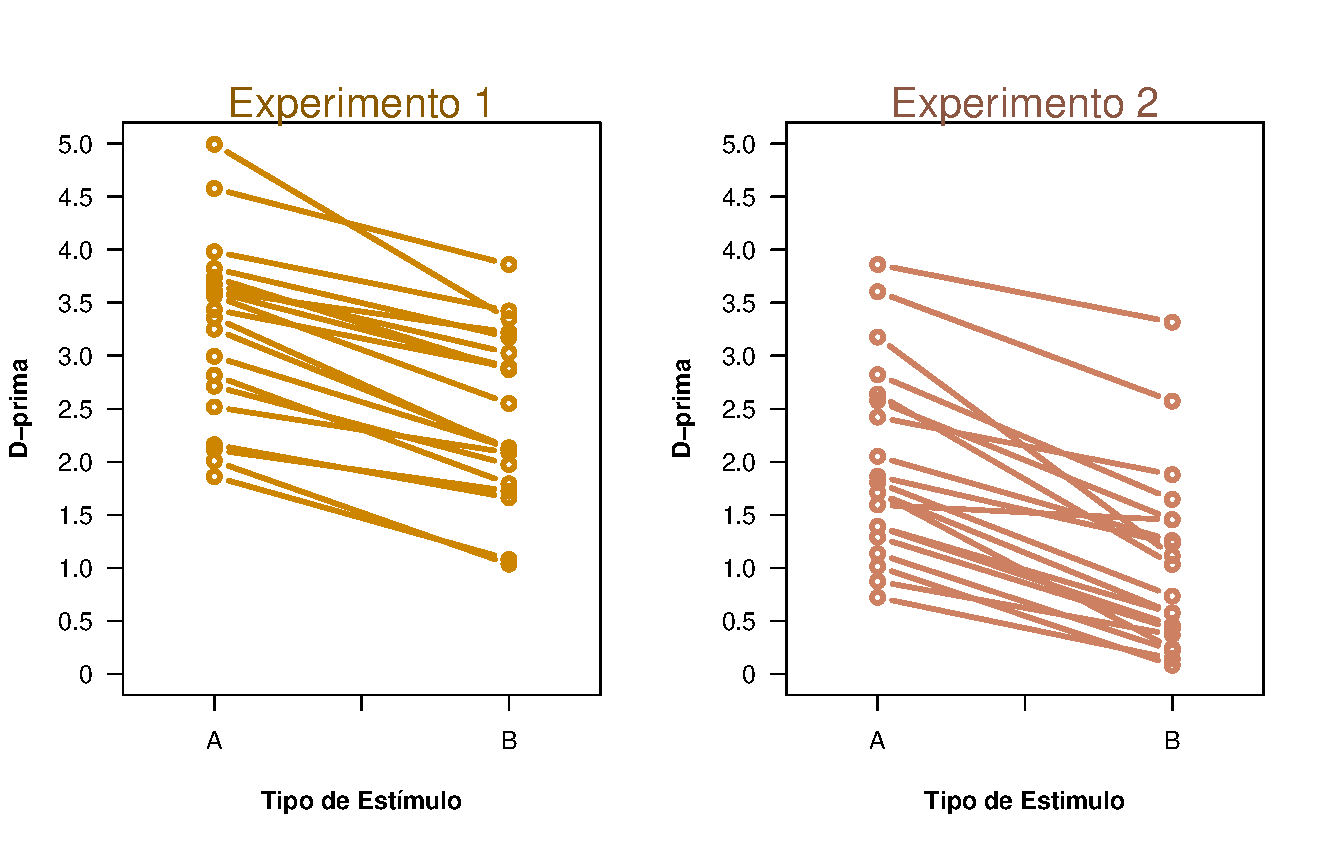
\includegraphics[width=0.90\textwidth]{Figures/Diff_D_E1yE2}
%\decoRule
\caption[Diferencias entre las $d'$ de los niveles de dificultad propuestos]{Por cada uno de los experimentos realizados se muestra la relación entre las $d'$ estimadas de acuerdo a la ejecución de cada participante. En ambos experimentos, se observa una tendencia sistemática a obtener niveles mayores de $d'$ en la clase A (la condición con pocos círculos en las figuras de Ebbinghaus).}
\label{fig:Diff_D}
\end{figure}

La Figura~\ref{fig:Diff_D} presenta de manera gráfica la comparación entre los valores de $d'$ estimados por cada nivel de dificultad de acuerdo con los datos obtenidos en los Experimentos 1 y 2, relacionando con una línea los pares de $d'$ estimados por cada participante ($d'(A) y d'(B)$). De acuerdo con esta figura, parece ser claro que las clases de estímulos propuestas cumplieron su objetivo, en tanto que puede apreciarse consistentemente la misma tendencia entre participantes a presentar valores mayores de $d'$ en la clase A que en la clase B.\\

A continuación se presentan los análisis realizados para determinar si las discrepancias que parecieran ser evidentes en la Figura~\ref{fig:Diff_D}, son estadísticamente significativas.\\

\textbf{Análisis Frecuentista: Prueba T para comparar las medias de $d'$ por nivel de dificultad}\\

Tal y como se reporta en los estudios que reportan evidencia del Efecto Espejo en Memoria de Reconocimiento, se realizó una prueba t para comparar la precisión con que los participantes discriminaron los estímulos Señal y los estímulos Ruido de cada clase de estímulos construida. Para ello, se computaron los valores de $d'$ correspondientes al desempeño de los participantes en cada nivel de dificultad y se comparó la diferencia entre los promedios de los valores obtenidos.\\

La Tabla~\ref{Tabla_t-Dprimas} presenta el promedio de las $d'$ computadas por cada nivel de dificultad en cada uno de los experimentos realizados, la diferencia en estas y un indicador sobre su significancia estadística. Como se puede apreciar, la diferencia entre las medias de $d'$ estimadas es significativa en ambos experimentos.\\

\begin{table}
\caption[Prueba T para evaluar las diferencias entre las medias de $d'$ por nivel de dificultad]{Pruebas t para evaluar las diferencias entre las medias de $d'$ computadas por nivel de dificultad}
\label{Tabla_t-Dprimas}
\centering
\begin{tabular}{l | c c c c}
\toprule
%\tabhead{Groups} & \tabhead{Treatment X} & \tabhead{Treatment Y} \\
\textbf{Experimento} & \textbf{$\mu d'(A)$} & \textbf{$\mu d'(B)$} & \textbf{T}  & \textbf{P value}\\
\midrule
Experimento 1 & 3.240 & 2.448 & -3.0587 & 0.0020 \\
Experimento 2 & 1.981 & 1.038 & -3.4131 & 0.0007 \\
\bottomrule
\end{tabular}
\end{table}


\textbf{Análisis Bayesiano: Modelo jerárquico bayesiano para evaluar las diferencias en $d'$}\\

Partiendo del modelo bayesiano estándar que describe los supuestos realizados por la SDT, (Lee y Wagenmakers, \citeyear{LeeBook}), se desarrolló un modelo jerárquico bayesiano (identificado dentro del presente trabajo como Modelo Delta), que asume que tanto los valores de $d'$, como el sesgo $c$ estimado por cada nivel de dificultad se distribuyen de acuerdo a una distribución normal, de donde se extraen los valores computados por cada participante. Bajo este supuesto, el modelo utiliza las inferencias realizadas sobre los valores de $d'$ y $c$ que subyacen al desempeño de cada sujeto para estimar los parámetros que definen la distribución normal de donde se asume que éstos son extraidos (la media ($\mu$) y la desviación estándar ($\sigma$)). Finalmente, el modelo incorpora un parámetro $\delta$ que computa la diferencias entre las medias de las $d'$ estimadas por concidión.\\

\begin{figure}[th]
\centering
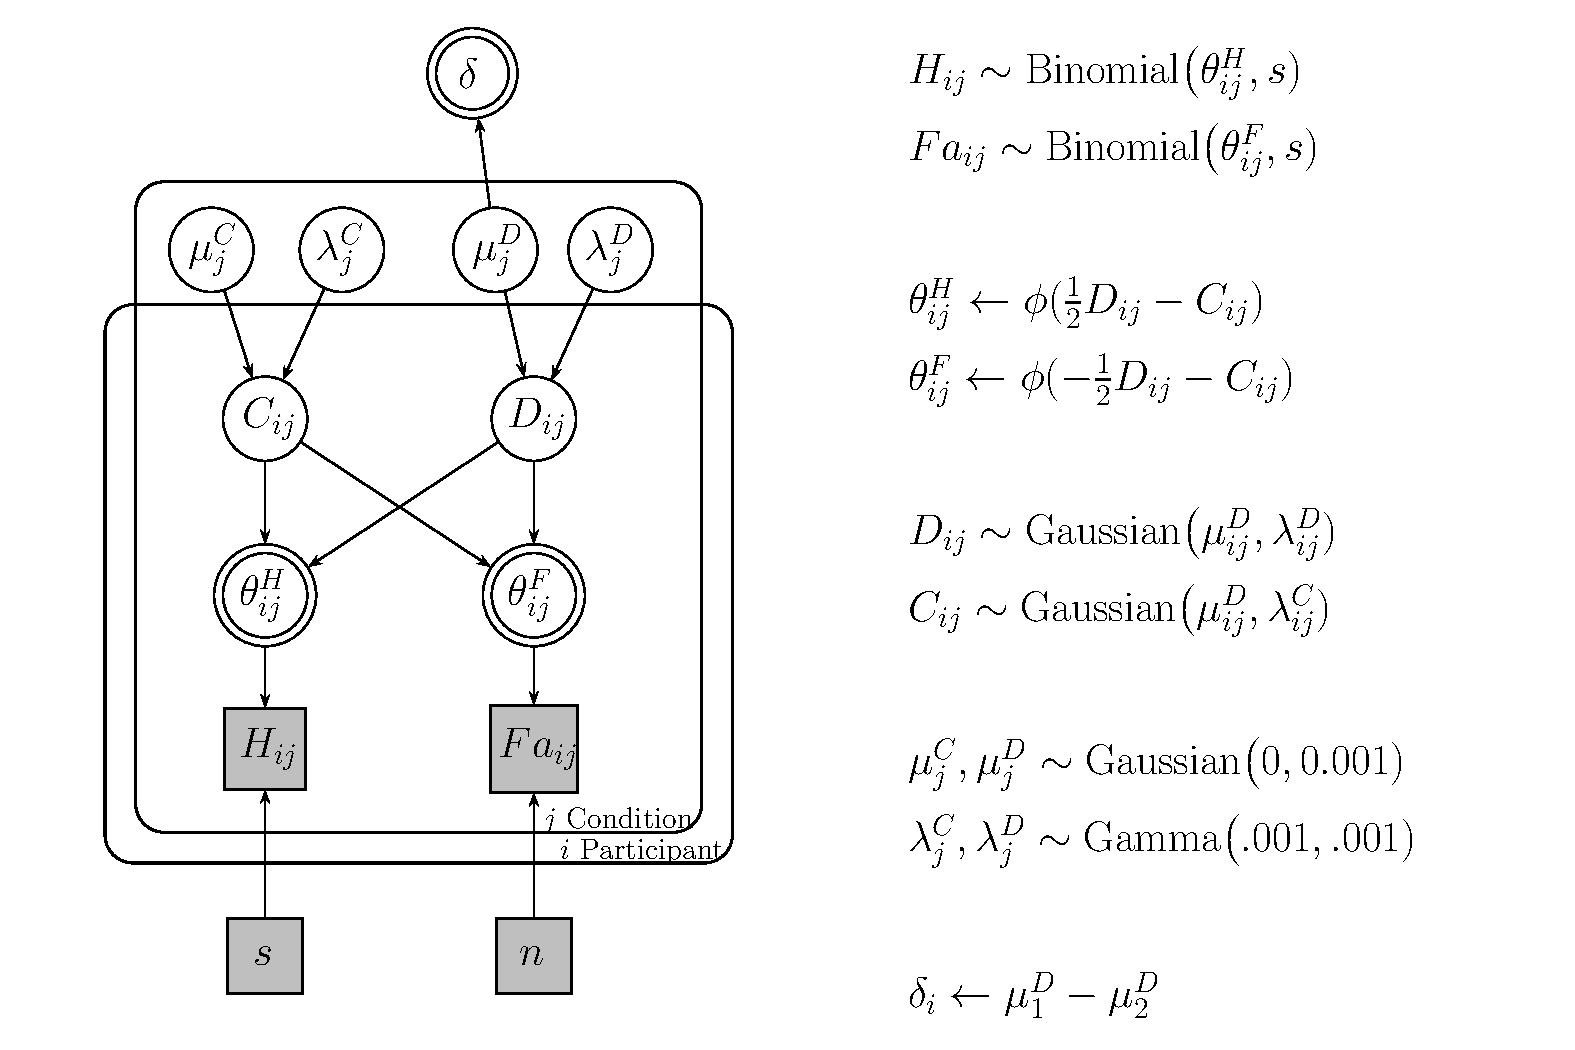
\includegraphics[width=1.1\textwidth]{Figures/Model_Delta_Diff_D}
%\decoRule
\caption[Modelo Delta: Modelo jerárquico bayesiano para revisar las diferencias en $d'$ entre clases de estímulos]{Modelo jerárquico bayesiano que asume que la $d'$ y la medida de sesgo $c$ computada por cada participante en cada clase de estímulo proviene de una distribución normal. El modelo incorpora un parámetro ($\delta$) que estima la diferencia entre las medias de $d'$ estimadas por cada condición. El modelo tiene priors no informativas.}
\label{fig:Mod_Delta}
\end{figure}

La Figura~\ref{fig:Mod_Delta} ilustra las relaciones y parámetros definidos en el modelo desarrollado. A este tipo de representaciones, se les conoce como \textit{Modelos Gráficos} y en el caso del Modelo Delta aquí presentado, se presentan los siguientes elementos:\\

\begin{itemize}
\item \underline{Nodos sombreados que representan los datos.}\\

En los modelos gráficos, los nodos representan las variables que el modelo a representar asume tienen una influencia sobre el proceso cognitivo de interés. Dependiendo cómo estén dibujados, los nodos proporcionan información sobre la naturaleza de dichas variables en torno a tres grandes puntos: 1) la variable adopta valores contínuos (nodo circular) o discretos (nodo cuadrado); 2) el valor de la variable es conocido (nodo sombreado) o necesita ser inferido a partir de los datos (nodo claro), y 3) la variable es probabilística (nodo simple) o está determinada por el valor inferido de otras variables (doble nodo), (Lee y Wagenmakers, \citeyear{LeeBook}).\\

En el caso de nuestros experimentos, los datos registrados de manera directa -a partir de los cuales se desarrolla todo el análisis- son el número de ensayos con Ruido ($n$) y Señal ($s$), y los resultados obtenidos en la tarea: el número total de Hits ($H_ij$) y Falsas Alarmas (($Fa_ij$) cometidos por cada participante ($i$) en cada condición ($j$).\\

\item \underline{Las tasas de Hits y Falsas Alarmas como una probabilidad oculta.}\\ 

Mientras que en la literatura clásica en SDT las tasas registradas de Hits y Falsas Alarmas son interpretadas como reflejo directo del área de las distribuciones de Señal y Ruido que caen por encima del criterio de elección, (Wickens, \citeyear{Wickens1}; Gescheider, \citeyear{Gescheider}; Stainslaw y Todorov, \citeyear{Stainslaw1999}, bajo el marco del modelamiento bayesiano, el total registrado de Hits y Falsas Alarmas ($H_ij$ y $Fa_ij$) se toma una instancia de un conteo de casos específicos encontrados dentro de un conjunto de observaciones ($s$ y $n$, respectivamente) con cierta probabilidad ($\theta^H_{ij}$ y $\theta^F_{ij}$).\\

En otras palabras, el modelo bayesiano propuesto asume que $H_ij$ y $Fa_ij$ representan un \textit{'número de éxitos'} extraídos con una probabilidad oculta de un conjunto definido de observaciones, de acuerdo a una distribución binomial con parámetros $p=$ ($\theta^H_{ij}$ o $\theta^F_{ij}$) y $n=$ ($s$ o $n$). Es decir:\\

\begin{center}
$H_{ij}\sim \mathrm{Binomial}\bigl(\theta^H_{ij}, s)$
y
$F_{ij}\sim \mathrm{Binomial}\bigl(\theta^F_{ij}, n)$\\
\end{center}

\item \underline{Sesgo y Discriminabilidad}\\

De acuerdo con la SDT, la probabilidad que determina las tasas registradas de Hits y Falsas Alarmas ($\theta^H_{ij}$ y $\theta^F_{ij}$) representan el área de las distribuciones de Señal y Ruido que caen por encima de los criterios de elección utilizados por los participantes. Es decir, que dicha probabilidad está definida como la función de densidad acumulada (CDF, por sus siglas en inglés, típicamente representada con el parámetro $\phi$) en una distribución normal estándar para la ubicación de $x$ que corresponde a la diferencia entre $\frac{1}{2}D_{ij}$ (en el caso de los Hits) o $\frac{1}{2}D_{ij}$ (en el caso de las Falsas Alarmas), y la medida de sesgo $C_{ij}$. Es decir:\\

\begin{center}
$\theta^H_{ij}\gets \phi (\frac{1}{2}D_{ij}-C_{ij})$
y
$\theta^F_{ij}\gets \phi (-\frac{1}{2}D_{ij}-C_{ij})$\\
\end{center}

\item \underline{Plato de participantes}\\

En los modelos gráficos bayesianos se utilizan platos para representar lo que en cualquier lenguaje de programación se conoce como un \textit{ciclo for}, (Lee y Wagenmakers, \citeyear{LeeBook}). Es decir, los platos delimitan conjuntos de parámetros cuyo cómputo se realizará tantas veces como casos -o conjuntos de datos- represente el plato. Por ejemplo, un plato $a$ que contiene los parámetros $p_1, p_2... p_n$ indica que el cómputo de estos se realizará por cada caso contenido en $a$.\\

En el caso del modelo desarrollado, el primer plato ($i$ $participantes$) señala que el cómputo de las probabilidades ocultas tras la emisión de cada par de Hits y Falsas Alarmas registrado ($\theta^H_{ij}$ y $\theta^F_{ij}$) y la estimación del valor de los parámetros $D_{ij}$ y $C_{ij}$ que mejor permitan dar cuenta de dichas probabilidades a partir de la CDF de un par de distribuciones normales, se va a repetir y realizar por cada uno de los participantes ($i$) incluidos en el experimento -es decir, por cada par de Hits y Falsas Alarmas recolectado-.\\

No hay necesidad de incluir los parámetros $n$ y $s$, que representan el total de ensayos con Ruido y Señal contenidos en el experimento, ya que estos permanecen constantes para todos los participantes ($i$) y para todas las clases de estímulos ($j$).\\

\item \underline{Estructura jerárquica: Distribuciones que describen los datos individuales}\\

Como ya se mencionó, la cualidad esencial del modelo desarrollado es que asume que los parámetros $D_{j}$ y $C_{j}$ computados por cada sujeto $i$ provienen de distribuciones normales que describen la discriminabilidad ($d'$) y el sesgo en las respuestas ($c$) asociado a cada clase de estímulos $j$. Dichas distribuciones están definidas por los parámetros $\mu^D_{j}$, $\mu^C_{j}$ y $\sigma^D_{j}$, $\sigma^C_{j}$, que el modelo infiere a partir de los datos ($H_ij$ y $Fa_ij$). Es decir:\\

\begin{center}
$D_{ij}\sim \mathrm{Gaussian}\bigl(\mu^D_{j},\lambda^D_{j})$\\
y\\
$C_{ij}\sim \mathrm{Gaussian}\bigl(\mu^C_{j},\lambda^C_{j})$\\
\end{center}

\item \underline{Plato de Condición}\\

Un segundo plato ($j$ $condiciones$) señala que el cómputo de los parámetros que definen las distribuciones normales asociadas al sesgo y la discriminabilidad, se va a realizar de manera independiente para cada clase de estímulo, a partir del par de Hits y Falsas Alarmas registrado para cada uno por cada participante ($plato$ $i$ $participantes$).\\

\item \underline{Parámetro Delta}\\

Finalmente, se incluye un parámetro Delta ($\delta$) que computa directamente la diferencia entre las inferencias realizadas acerca del valor de las medias de $d'$ por cada nivel de dificultad, ($\mu^D_{A}$ y $\mu^D_{B}$). Es decir:\\

\begin{center}
$\delta \gets \mu^D_{A}-\mu^D_{B}$\\
\end{center}

El parámetro $\delta$ está representado con un doble nodo para señalar que es un parámetro determinado por los valores estimados para otras variables ($\mu^D_{A}$ y $\mu^D_{B}$) de manera directa -no probabilística-.\\
\end{itemize} 

En la Figura~\ref{fig:Delta_Joints} se presentan las densidades de probabilidad posterior marginales y conjunta, para las inferencias realizadas en cuanto al valor de las medias de las distribuciones de $d'$ y $c$ por cada condición, en cada uno de los Experimentos llevados a cabo, (Experimento 1 en el panel superior y Experimento 2 en el inferior). En los extremos de cada gráfica se presenta la densidad de probabilidad marginal computada para la media de cada parámetro a lo largo de distintos valores, distinguiendo con colores las clases de estímulos diseñadas (en azul se presenta la clase fácil A y en púrpura, la clase difícil B). El panel central presenta las densidades de probabilidad posterior conjuntas entre distintos pares de valores para $\mu d'$ y $\mu c$. Los colores empleados en estos gráficos serán utilizados recurrentemente durante la presentación de los resultados y su análisis para diferenciar la clases A y B.\\ 

\begin{figure}[th]
\centering
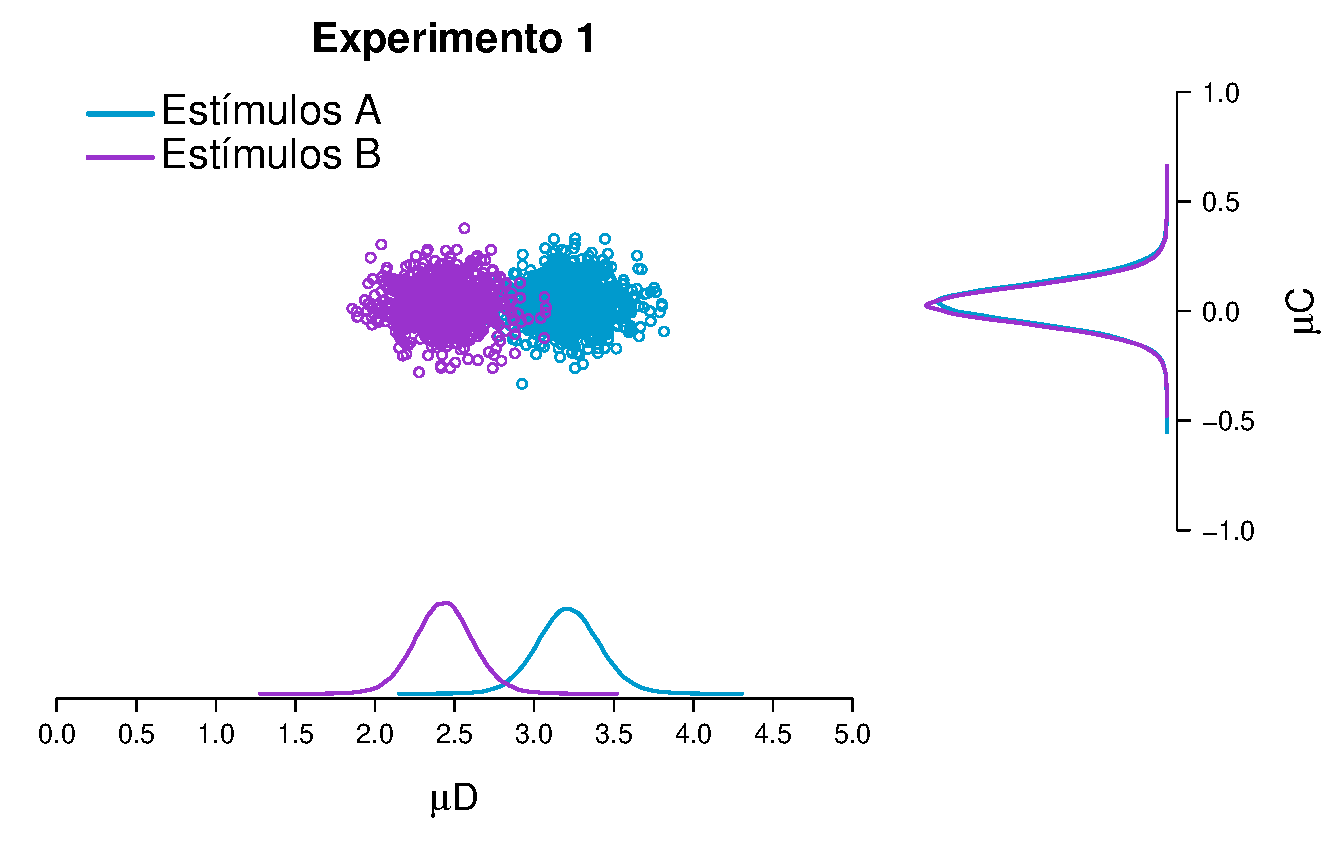
\includegraphics[width=0.7\textwidth]{Figures/MDelta_Joint_E1}\\
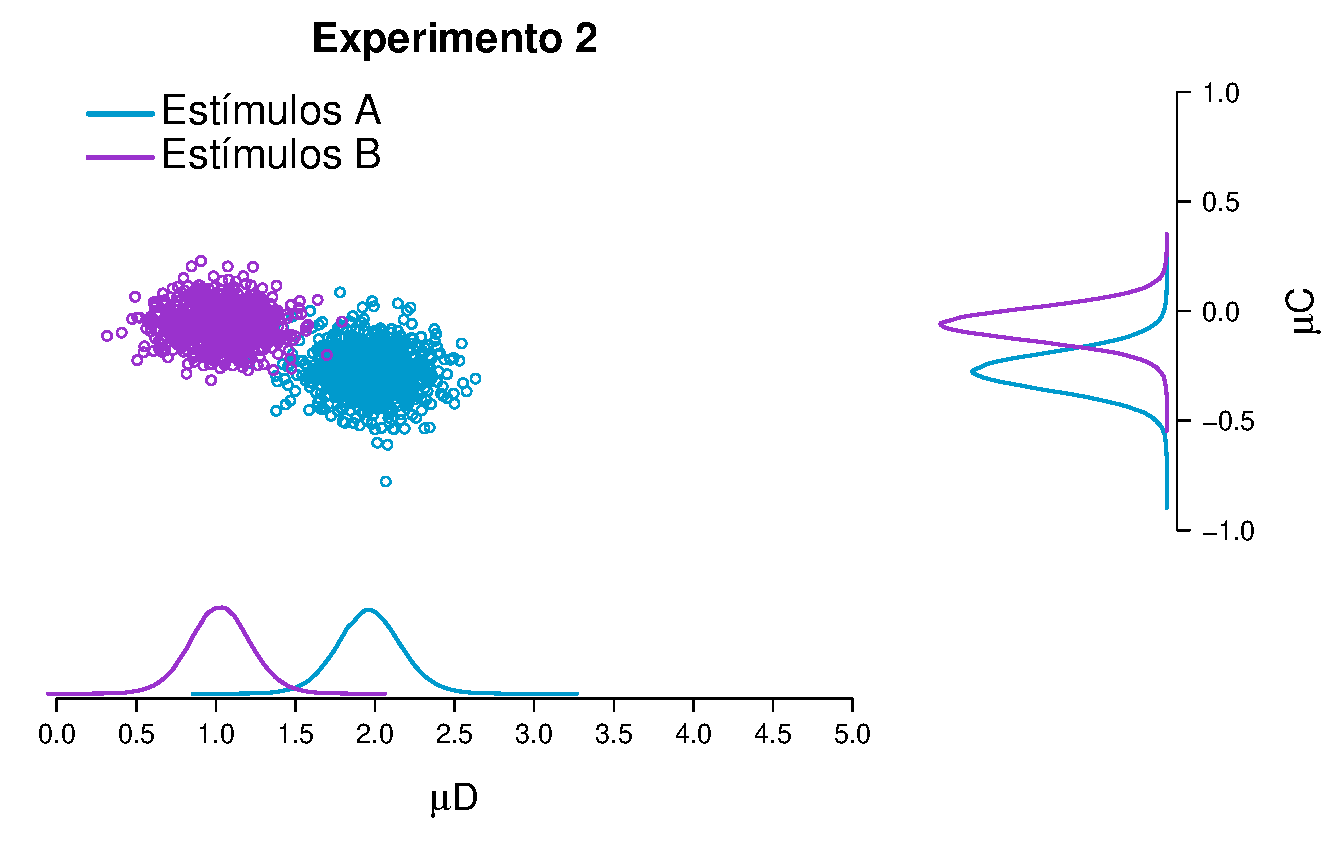
\includegraphics[width=0.7\textwidth]{Figures/MDelta_Joint_E2}\\
%\decoRule
\caption[Modelo Delta: Distribuciones posteriores marginales y conjuntas para $\mu d'$ y $\mu c$ por cada clase de estímulo]{Se presenta la densidad posterior conjunta y marginal computada por el Modelo Delta para las medias de $d'$ y $c$ de cada clase, por cada experimento realizado.}
\label{fig:Delta_Joints}
\end{figure}

De acuerdo con la Figura~\ref{fig:Delta_Joints} parece ser que, en general, los valores estimados por el modelo para las medias de $d'$ en cada clase de estímulo son de hecho diferentes. Esto se puede observar tanto en las distribuciones de densidad marginal trazadas por cada clase de estímulo, que se sobrelapan sobre un rango pequeño de valores y con baja probabilidad, como en la distribución de los puntos trazados por cada pareja de valores inferidos de $d'$ y $c$ por cada clase de estímulo, donde se puede distinguir con facilidad dos aglomeraciones de puntos estimados: las inferencias realizadas para la clase A, que tiende a tener valores más bajos de $\mu d'$ y las inferencias sobre la clase B, con valores $\mu d'$ más altos. La distancia entre los valores de $\mu d'(A)$ y $\mu d'(B)$ estimados es mayor en el Experimento 1, donde sólo se presentó una ilusión de Ebbinghaus por ensayo.\\


Es interesante señalar que, de acuerdo con las inferencias presentadas en la Figura~\ref{fig:Delta_Joints}, los valores estimados para $\mu c$ por cada clase de estímulo se despliegan en un mismo rango de valores, siendo que las densidades posteriores marginales se encuentran completamente sobrelapadas. Más interesante aún es notar que, de acuerdo con las estimaciones del modelo, los participantes en el Experimento 1 no mostraron sesgo alguno al responder a los estímulos de la tarea. Por otro lado, en el Experimento 2 se aprecian diferencias en el sesgo promedio estimado para cada clase de estímulos, siendo que para la clase A presenta un sesgo liberal, mientras que para la clase B se sugiere un sesgo neutro -tal y como se reportó en el Experimento 1-.\\

Para evaluar la variabilidad de los valores de $d'$ y $c$ computados por cada participante para cada clase de estímulo, las Figuras~\ref{fig:Delta_Dprima} y \ref{fig:Delta_Cbias} presentan las densidades de probabilidad posterior computadas por cada par de Hits y Falsas Alarmas registrado en cada una de las clases de estímulos. En estas Figuras se presenta además, con una línea más gruesa, la densidad de probabilidad de los valores estimados para las medias de cada parámetro para las clases A y B.\\

\begin{figure}[th]
\centering
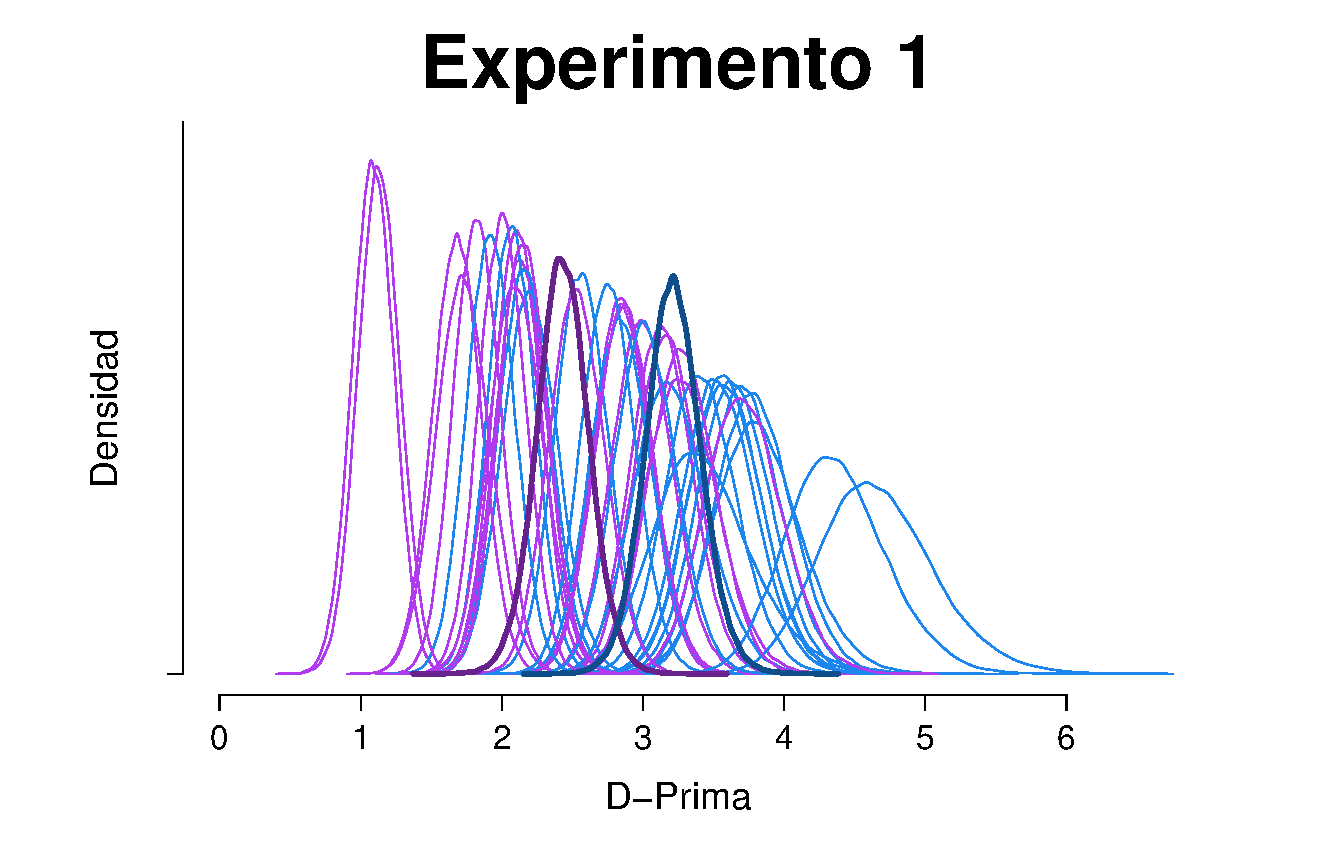
\includegraphics[width=0.6\textwidth]{Figures/MDelta_Dprima_E1}\\
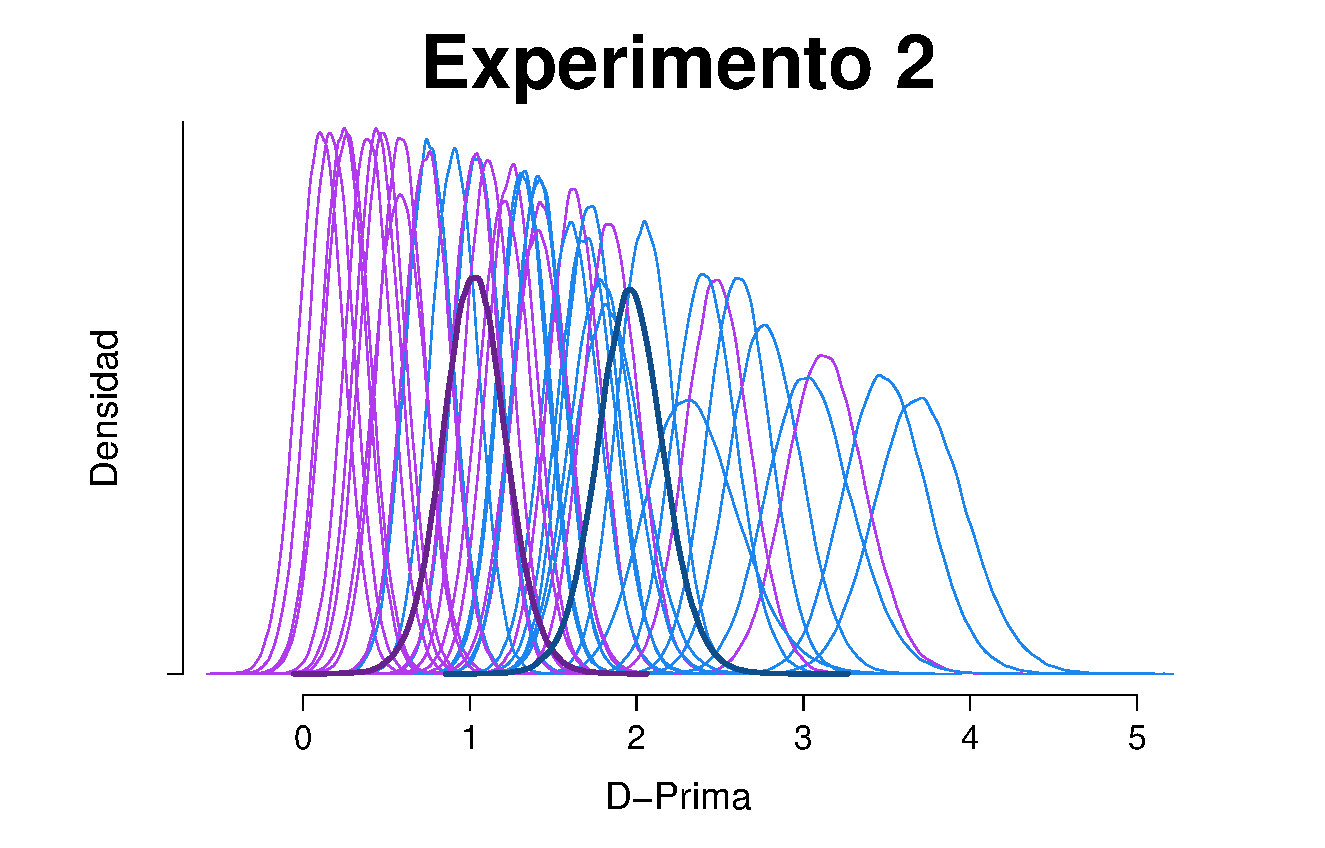
\includegraphics[width=0.6\textwidth]{Figures/MDelta_Dprima_E2}\\
%\decoRule
\caption[Modelo Delta: Densidades posteriores de los valores de $d'$ estimados individualmente y en promedio, por experimento]{Densidades posteriores de los valores de $d'$ y estimados por el Modelo Delta por cada clase de estímulo (azul A, purpura B), individualmente (líneas delgadas) y en promedio (líneas gruesas)}
\label{fig:Delta_Dprima}
\end{figure}

En la Figura~\ref{fig:Delta_Dprima} se presentan las estimaciones realizadas por cada participante acerca del valor de $d'$ que mejor describe su desempeño ante cada clase de estímulo, distinguiendo en paneles distintos los valores estimados en el Experimento 1 (panel superior) y 2 (panel inferior). De acuerdo con las densidades de probabilidad posterior estimadas por cada par de Hits y Falsas Alarmas registrado, puede observarse que en el extremo derecho -que corresponde con valores de $d'$ altos que indican una alta discriminabilidad- se encuentran una mayor cantidad de inferencias realizadas para la clase fácil A, en tanto que en el extremo izquierdo -valores bajos de $d'$ que sugieren una baja discriminabilidad- se concentra una mayor cantidad de distribuciones de densidad correspondientes al cómputo realizado para la clase difícil B. De manera adicional, la figura presenta con líneas más gruesas los valores estimados para las medias de $d'$ en cada condición, permitiendo que su exploración sea realizada a la luz de la variabilidad capturada por las estimaciones individuales.\\

\begin{figure}[th]
\centering
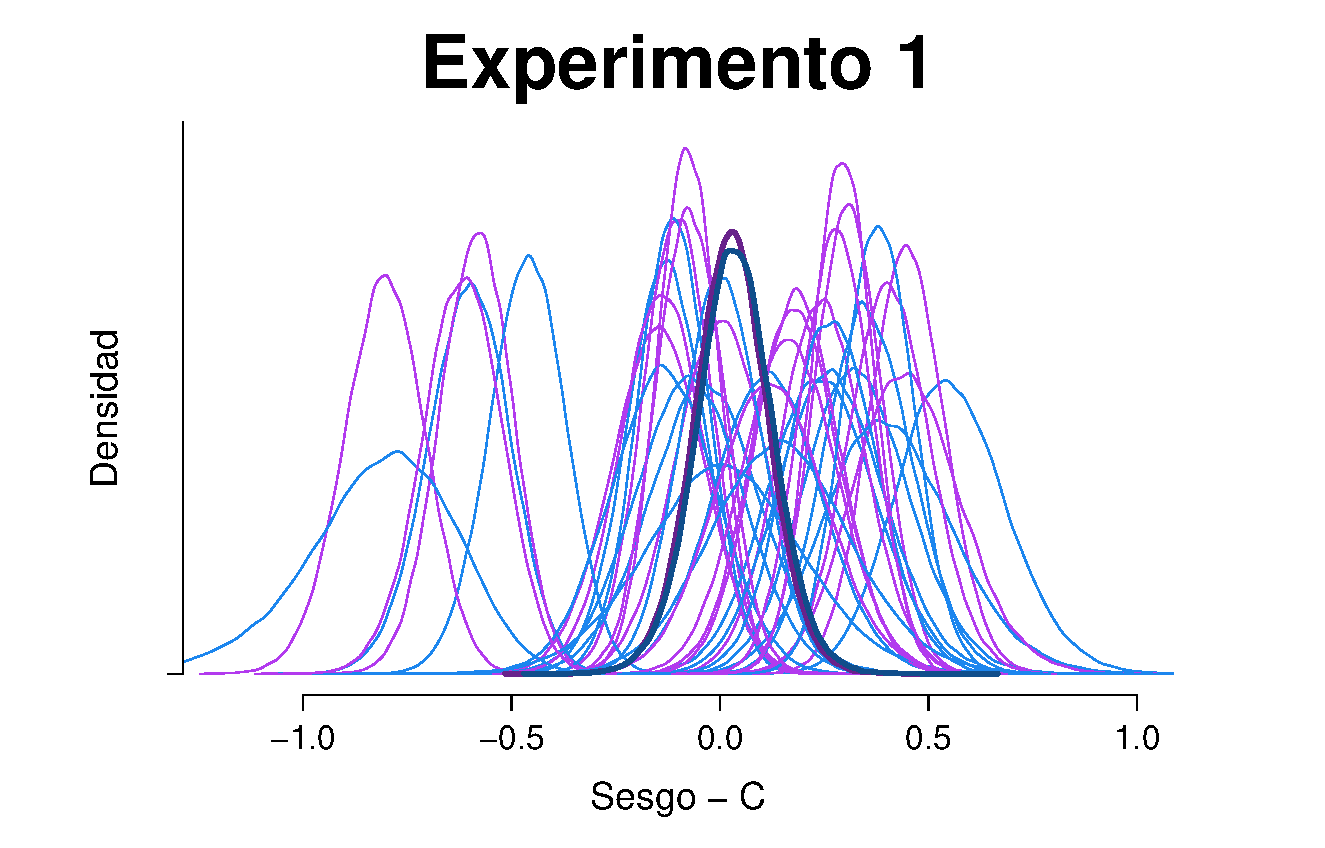
\includegraphics[width=0.6\textwidth]{Figures/MDelta_Cbias_E1}\\
\includegraphics[width=0.6\textwidth]{Figures/MDelta_Cbias_E2}\\
%\decoRule
\caption[Modelo Delta: Densidades posteriores de los valores de $c$ estimados individualmente y en promedio, por experimento]{Densidades posteriores de los valores de $c$ y estimados por el Modelo Delta por cada clase de estímulo (azul A, purpura B), individualmente (líneas delgadas) y en promedio (líneas gruesas)}
\label{fig:Delta_Cbias}
\end{figure}

Por su parte, en cuanto a los valores del parámetro $c$ estimados por cada participante, en la Figura~\ref{fig:Delta_Cbias} se pueden apreciar diferencias en términos de las inferencias realizadas a partir de los datos recopilados en cada experimento. En el Experimento 1, pese a la variabilidad en las estimaciones realizadas, no parece haber ninguna relación entre el tipo de estímulo y los valores de $c$ estimados, tal y como se ilustra con el sobrelape total en que se presentan las densidades de probabilidad posterior estimadas para las medias de ambos grupos. Por otro lado, en el caso del Experimento 2 sí parece haber una ligera diferencia en términos del sesgo con que los participantes responden a cada clase de estímulos, siendo que en general se observan valores de $c$ por debajo de 0 (sesgo liberal) en los estímulos de la clase A, mientras que en la clase B se observa la misma ausencia de sesgo ($c$ cercano a $0$) que en los estímulos presentados en el Experimento 1.\\

Finalmente, la Figura~\ref{fig:Delta} presenta la densidad de probabilidad posterior computada para las diferencias entre las medias de $d'$ computadas por cada condición, que se traducen en distintos valores del parámetro $\delta$. Tal como se puede apreciar en la figura, parece ser que a la luz de los datos registrados en los dos experimentos realizados, es muy poco probable que la diferencia entre las $d'$ asociadas a cada clase de estímulo sea 0. De acuerdo con las gráficas presentadas, los picos más altos de densidad de probabilidad aparecen cerca de 1, lo que sugeriría que la media de las $d'$ asociadas a cada clase de estíimulos difieren alrededor de una unidad de desviación estándar.\\

\begin{figure}[th]
\centering
\includegraphics[width=0.6\textwidth]{Figures/MDelta_DensidadDelta_E1}\\
\includegraphics[width=0.6\textwidth]{Figures/MDelta_DensidadDelta_E2}\\
%\decoRule
\caption[Modelo Delta: Densidad posterior de los valores estimados para el parámetro Delta en cada Experimento]{Densidad posterior computada en cada experimento respecto de los valores de Delta, que refiere a la diferencia entre las medias estimadas de $d'$ por cada clase de estímulos.}
\label{fig:Delta}
\end{figure}

En conjunto, los análisis de datos realizados arrojaron evidencia a favor de la manipulación experimental implementada en el diseño de los estímulos construidos para formar los dos niveles de dificultad a comparar. Se confirmó la existencia de una diferencia significativa en la discriminabilidad ($d'$) asociada a cada clase de estímulos, que además se reportó de acuerdo a lo esperado con base en la literatura revisada para el diseño de los estímulos: las figuras de Ebbinghaus compuestas por un número menor de círculos externos (clase A), tuvieron valores de $d'$ más grandes que las figuras de la clase B, formados por un número mayor de círculos externos.\\

Una vez comprobada la relación $d'(A) > d'(B)$, se prosiguió a evaluar la presentación de los patrones de respuesta identificados como Efecto Espejo en Memoria de Reconocimiento, en los datos obtenidos en el presente trabajo.\\












\subsection{Diferencias en las Tasas de Hits y Falsas Alarmas}

Como se recordará de la revisión presentada en el Capítulo 1 acerca del fenómeno identificado como Efecto Espejo en Memoria de Reconocimiento, la evidencia en favor del mismo se presenta en Tareas de respuesta binaria Sí/No a partir del siguiente patrón de respuestas:\\
 
\begin{center}
$FA(A) < FA(B) < H(B) < H(A)$\\
\end{center}
\begin{center}
donde $FA$ y $H$ señalan las tasas de Hits y Falsas Alarmas observadas durante la tarea en cada clase, (Glanzer y cols., \citeyear{Glanzer1993}).\\
\end{center}

Para evaluar la presentación de dicho patrón en los datos obtenidos en el presente estudio, se comparó el número de Hits y Falsas Alarmas cometidos en cada una de las clases de estímulos construidas por cada participante.\\

Una forma sencilla de explorar dicha relación fue mediante la realización de gráficas de barras que presentaran las diferencias en los resultados obtenidos por los participantes para los distintos tipos de estímulos presentados. Como un caso ejemplar, en la Figura~\ref{fig:MirrorRate_E2_P4} se muestra la frecuencia absoluta de Hits y Falsas Alarmas obtenidas por el Participante 4 en el Experimento 2, por cada clase de estímulos construido, distinguiendo la clase fácil A en color azul y la clase difícil B, en púrpura; presentando el patrón de respuestas identificado como Efecto Espejo. Las gráficas correspondientes al desempeño del resto de los participantes en los Experimentos 1 y 2, pueden consultarse en los Apéndices.\\
\\

\begin{figure}[th]
\centering
\includegraphics[width=0.60\textwidth]{Figures/MirrorRate_Exp2_P4}
%\decoRule
\caption[Diferencias entre Hits y Falsas Alarmas por Condición; Participante ejemplar]{Gráfica de barras que presenta el número de Hits y Falsas Alarmas cometidos por el Participante 4 del Experimento 2 en cada clase de estímulo, (clase fácil A en azul y clase difícil B en púrpura). Los resultados se presentan de acuerdo al órden ascendente entre los resultados reportados en el Efecto Espejo.}
\label{fig:MirrorRate_E2_P4}
\end{figure}


La comparación global entre las tasas de Hits y Falsas Alarmas registradas por cada participante de los Experimentos 1 y 2 en cada tipo de estímulo se presenta en la Figura~\ref{fig:Diff_Rate}. De acuerdo con el patrón de respuestas reportado como parte del Efecto Espejo, se espera observar una pendiente descendente para la comparación de las tasas de Hits registradas por cada condición (paneles izquierdos) y una pendiente ascendente en el registro de tasas de Falsas Alarmas (paneles derechos). Como se puede observar, parece ser que dichas tendencias aparecen en la mayoría de los participantes, presentándose de manera más evidente en los datos registrados en el Experimento 1. Sin embargo, resulta poco claro si las diferencias entre las tasas registradas en una y otra clase de estímulos son lo suficientemente grandes como para considerarse estadísticamente significativas.\\

\begin{figure}[th]
\centering
\includegraphics[width=0.65\textwidth]{Figures/Diff_Rate_E1}\\ 
\includegraphics[width=0.65\textwidth]{Figures/Diff_Rate_E2}\\
%\decoRule
\caption[Diferencias entre las Tasas de Hits y Falsas Alarmas registradas en cada clase de estímulos]{Se presenta la comparación, participante a participante, entre las tasas de Hits y Falsas Alarmas registradas para cada clase de estímulo, (paneles izquierdos y derechos, respectivamente). El panel superior muestra las comparaciones correspondientes al Experimento 1 y el panel inferior, al Experimento 2.}
\label{fig:Diff_Rate}
\end{figure}

A continuación se presentan los análisis realizados para determinar si los Hits y las Falsas Alarmas registrados por cada clase de estímulos son estadísticamente diferentes.\\

\textbf{Análisis Frecuentista: Pruebas T para comparar las tasas de Hits y Falsas Alarmas registradas por cada clase de estímulos}\\

De acuerdo con la literatura, la manera más apropiada de evaluar la significancia estadística del patrón de respuestas reportado como Efecto Espejo en Tareas de respuesta Sí/No, es mediante la realización de dos pruebas-T que evalúen de manera independiente las diferencias entre las medias de las tasas de Hits reportadas por cada clase de estímulo y entre las tasas de Falsas Alarmas, (Glanzer y Adams, \citeyear{Glanzer1990}).\\

%Las pruebas t realizadas para evaluar la significancia estadística de las diferencias encontradas entre los promedios de las tasas computadas, se enfrentan con el problema de que los datos a comparar se encuentran restrigidos dentro de un rango de $0$ a $1$. Más aún, de acuerdo con los supuestos de la SDT sobre el despliegue de las distribuciónes de Ruido y Señal sobre el eje de evidenncia, las tasas de ejecución se presentan dentro de rangos aún más restringidos, siendo que los aciertos (Hits y Rechazos Correctos) caen por arriba del $0.5$, y los errores (Omisiones y Falsas Alarmas), por debajo. Esto representa un problema para la comparación de los resultados encontrados, porque puede darse el caso de que las diferencias entre los datos registrados no sean lo suficientemente grandes como para considerárseles significativas, con independencia de si se presentan de forma consistente en la mayoría de los datos individuales.\\

%Para solucionar el problema del efecto de suelo y techo que podría estar mermando la evaluación de los datos obtenidos como evidencia del impacto de la manipulación experimental sobre el desempeño de los participantes, los datos crudos a comparar suelen transformarse a una nueva Escala, de manera que la distancia entre estos aumente, pero manteniendo la proporción de los mismos intacta. En el caso específico de la literatura que aborda el Efecto Espejo en Memoria de Reconocimiento, se ha optado por implementar una transformación arcoseno de las tasas de respuesta registradas antes de someterlas al análisis estadístico.\\

%De acuerdo con las pruebas t realizadas en el presente estudio para comparar los promedios de las transformaciones arcoseno de las tasas de ejecución registradas por cada clase de estímulo, se encontraron diferencias significativas en la ejecución de los participantes a la tarea Sí/No dependientes de la clase de estímulo a evaluar en ambos experimentos, reportándose diferencias altamente significativas entre las tasas de Hits y diferencias apenas significativas (justo por debajo de $p=0.05$) para las tasas de Falsas Alarmas.\\

Además, para prevenir el efecto de suelo y techo causado por el hecho de que los datos a comparar éstán restringidos dentro de un rango entre $0$ y $1$, en la literatura se recomienda hacer una transformación arcoseno de las tasas registradas de Hits y Falsas Alarmas por cada clase de estímulos, (Glanzer y Adams, \citeyear{Glanzer1990}).\\ 

En la Tabla~\ref{Tabla_t-HitsyFA} se presentan los resultados obtenidos en la prueba-T de muestras independientes realizada para evaluar las diferencias entre las medias de las tasas de Hits y Falsas Alarmas obtenidas entre cada clase de estímulo, por cada Experimento realizado. En la tabla se muestra tanto la media de las tasas crudas registradas, como de su transformación arcoseno.\\

\begin{table}
\caption[Prueba T para evaluar diferencias entre las tasas de ejecución (Hits y F. Alarmas) promedio registradas por cada condición]{Se presentan los resultados de las pruebas t de una muestra realizadas para la comparación del promedios de las transformaciones arcoseno de las tasas registradas por cada clase de estímulos, en los Experimentos 1 y 2.}
\label{Tabla_t-HitsyFA}
\centering
\begin{tabular}{l l | c c c c c c}
\toprule
%\tabhead{Groups} & \tabhead{Treatment X} & \tabhead{Treatment Y} \\
\textbf{} & \textbf{Tasa} & \textbf{$\mu(A)$} & \textbf{$arcsin(\mu(B))$} & \textbf{$\mu(B)$} & \textbf{$arcsin(\mu(B))$} &\textbf{T} & \textbf{P value}\\
\midrule
Exp 1 & Hits & 0.922 & 1.314 & 0.860 & 1.209 & -2.4348 & 0.0098 \\
Exp 1 & FA & 0.08 & 0.247 & 0.143 & 0.353 & 1.872 & 0.0345 \\
Exp 2 & Hits & 0.857 & 1.219 & 0.681 & 0.994 & -3.3595, & 0.0009 \\
Exp 2 & FA & 0.266 & 0.524 & 0.336 & 0.611 & 1.7223 & 0.0468 \\
\bottomrule
\end{tabular}
\end{table}

De acuerdo con los resultados de las pruebas T presentadas en la Tabla~\ref{Tabla_t-HitsyFA}, las diferencias entre el promedio de las transformaciones arcoseno de las tasas de Hits y Falsas Alarmas registradas por cada clase de estímulo, son estadísticamente significativas en ambos experimentos.\\

\textbf{Análisis Bayesiano: Modelo bayesiano desarrollados para comparar las tasas de Hits y Falsas Alarmas entre clases de estímulos}\\

Cuando las mismas pruebas T presentadas en la Tabla~\ref{Tabla_t-HitsyFA} se realizan sin la transformación arcoseno de los datos, las diferencias entre las Tasas de Falsas Alarmas no resultan significativas en ningún experimento ($t=1.6536$, $p=0.0533>0.05$ para el Experimento 1 y $t=1.6577$, $p=0.0534>0.05$, para el Experimento 2). Esta discrepancia entre las conclusiones sugeridas por las pruebas t realizadas puede llegar a generar dudas acerca de su confiabilidad, aún cuando la transformación arcoseno se realiza de manera justificada, como una forma de prevenir el efecto de suelo y techo que pudiera afectar la evaluación de diferencias entre datos que se encuentren en la cercanía de los límites superior e inferior.\\

El desarrollo de un modelo bayesiano para evaluar las diferencias entre los Hits y las Falsas Alarmas registradas por cada clase de estímulo, presenta como ventaja principal que no requiere manipular los datos en forma alguna, en tanto que la estimación paramétrica se hace a partir de inferencias probabilísticas que evalúan qué valores de cada parámetro podrían dar cuenta de los datos registrados en conjunto con el resto de los paràmetros, con mayor probabilidad. Para ello, se desarrolló un modelo bayesiano (identificado en el presente trabajo como Modelo Tau), que incorpora un par de parámetros Tau ($\tau$) que computan las diferencias entre las estimaciones realizadas por cada clase de estímulos ($j$) acerca de las probabilidades ocultas tras la emisión de los Hits y Falsas Alarmas obtenidos por cada participante ($i$).\\ 

En la Figura~\ref{fig:Mod_Tau} se presenta el modelo gráfico correspondiente al Modelo Tau desarrollado para evaluar la evidencia del Efecto Espejo encontrada en los experimentos realizados. El modelo cuenta con los mismos elementos que el Modelo Delta desarrollado para comparar las medias de $d'$ por cada clase de estímulo, con las siguientes excepciones:\\

\begin{itemize}
\item \underline{El modelo Tau \textbf{no} asume una estructura jerárquica}\\

El Modelo Tau evalúa la diferencia entre las probabilidades ocultas tras la emisión de Hits y Falsas Alarmas en las clases A y B, por cada individuo. Este modelo no requiere de una estructura jerárquica porque tiene su énfasis en el cómputo determinista de las diferencias entre dos parámetros (las probabilidades ocultas tras los Hits y Falsas Alarmas de cada clase $\theta^H_{ij}$ y $\theta^F_{ij}$) que son a su vez definidos de manera determinista por la interacción de $D_{ij}$ y $C_{ij}$.\\

\item \underline{Parámetros Tau}\\

De la misma forma en que el Modelo Delta incorporaba un parámetro $\delta$ que computaba las diferencias entre las medias estimadas de $d'$ por cada clase de estímulo, el Modelo Tau recibe su nombre tras la inclusión de un par de parámetros Tau ($\tau^H_{i}$ y $\tau^F_{i}$) que determinan cuál es la diferencia entre las probabilidades ocultas tras la emisión de Hits y Falsas Alarmas por cada clase de estímulos:\\

\begin{center}
$\tau^H_{i}\gets \theta^H_{iA}-\theta^H_{iB}$\\
y\\
$\tau^F_{i}\gets \theta^F_{iB}-\theta^F_{iA}$\\
\end{center}

\end{itemize}

\begin{figure}[th]
\centering
\includegraphics[width=1.1\textwidth]{Figures/Model_Tau_Diff_Tetas}
%\decoRule
\caption[Modelo Tau: Modelo Bayesiano para evaluar las diferencias entre las tasas de Hits y Falsas Alarmas obtenidas por cada clase de estímulos]{Modelo bayesiano desarrollado para evaluar las diferencias entre las probabilidades ocultas tras la emisión de Hits y Falsas Alarmas para cada clase de estímulos}
\label{fig:Mod_Tau}
\end{figure}

En las Figuras~\ref{fig:Tau_Hits} y \ref{fig:Tau_FA} se presentan las inferencias realizadas por el Modelo Tau acerca de las probabilidades ocultas tras la producción de Hits y Falsas Alarmas de cada individuo, por cada clase de estímulos, en los Experimentos 1 y 2. \\

\begin{figure}[th]
\centering
\includegraphics[width=0.6\textwidth]{Figures/MTau_Hits_E1}\\
\includegraphics[width=0.6\textwidth]{Figures/MTau_Hits_E2}\\
%\decoRule
\caption[Modelo Tau: Inferencias individuales acerca de las probabilidades ocultas tras la emisión de Hits por clase de estímulos; Experimentos 1 y 2]{Se presentan las densidades de probabilidad posterior obtenidas individualmente para las probabilidades ocultas tras la emisión de Hits por cada clase de estímulos (clase fácil A en azul y clase difícil B, en púrpura).}
\label{fig:Tau_Hits}
\end{figure}

\begin{figure}[th]
\centering
\includegraphics[width=0.6\textwidth]{Figures/MTau_FA_E1}\\
\includegraphics[width=0.6\textwidth]{Figures/MTau_FA_E2}\\
%\decoRule
\caption[Modelo Delta: Inferencias individuales acerca de las probabilidades ocultas tras la emisión de Falsas Alarmas por clase de estímulos; Experimentos 1 y 2]{Se presentan las estimaciones individuales acerca de las probabilidades ocultas tras la emisión de Falsas Alarmas ante cada clase de estímulo (clase fácil A en azul y clase difícil B en púrpura).}
\label{fig:Tau_FA}
\end{figure}

Finalmente, en la Figura~\ref{fig:Tau} se presentan las densidades de probabilidad posterior para los valores de Tau ($\tau^H_{i}$ en tonalidades verdes y $\tau^F_{i}$ en tonos rojizos) computados por cada individuo en cada Experimento realizado. Cada panel incluído en esta Figura contiene una línea punteada que señala $\tau = 0$,  . Como se puede apreciar en la figura, las densidades de probabilidad estimadas para $\tau^H_{i}$ caen por encima del punto de \textit{'no diferencias'} para la mayoría de los participantes, en tanto que en el caso de las densidades de $\tau^F_{i}$ parece haber una mayor dispersión en el rango de valores estimados por cada participante y una mayor concentración de los mismos cae cerca del punto de \textit{'no diferencias'}.\\

\begin{figure}[th]
\centering
\includegraphics[width=0.6\textwidth]{Figures/MTau_DensidadTau_E1} \& \includegraphics[width=0.6\textwidth]{Figures/MTau_DensidadTau_E2}\\
%\decoRule
\caption[Modelo Tau: Densidades de probabilidad posterior para los valores de los parámetros Tau; Experimentos 1 y 2]{Se presentan las densidades de probabilidad posterior para las inferencias realizadas por el Modelo Tau acerca de las diferencias entre las probabilidades ocultas tras la emisión de Hits (Tau-Hits) y Falsas Alarmas (Tau-Falsas Alarmas) por cada clase de estímulos.}
\label{fig:Tau}
\end{figure}

Los resultados arrojados por el Modelo Tau confirman los hallazgos reportados con las pruebas t: la diferencia en el desempeño de los participantes ante cada clase de estímulos parece clara cuando se trata de comparar los Hits, pero no lo es tanto cuando se evalúan las Falsas Alarmas.\\

En el caso de las pruebas t realizadas para el análisis frecuentista, las tasas de Hits y Falsas Alarmas registradas son interpretadas directamente como un reflejo del área de las distribuciones de Ruido y Señal que caen por encima del criterio de elección (Stainslaw y Todorov, \citeyear{Stainslaw1999}) y la transformación arcoseno de las mismas aparece como un \textit{'mal necesario'} que, aún implicando una manipulación de los datos, compensa el impacto de los efectos de suelo y techo sobre la evaluación de las diferencias entre las tasas registradas (Glanzer y Adams, \citeyear{Glanzer1990}). \\ 

Por su parte, el modelamiento bayesiano de detección de señales permite una mayor flexibilidad en la interpretación de la ejecución de los participantes, pues el número de Hits y Falsas Alarmas son interpretadas como extracciones realizadas bajo la influencia de una probabilidad oculta, (Lee y Wagenmakers, \citeyear{LeeBook}). Por ello, los datos recopilados sobre la ejecución de los participantes no son tratados de manera determinista, sino probabilística, como el número de casos observados en un proceso binomial y no es necesario llevar a cabo ninguna manipulación adicional sobre los mismos para compensar la rigidez de su interpretación.\\

En cuanto al análisis de datos conducido en el presente estudio para evaluar la evidencia del Efecto Espejo encontrada en los experimentos realizados, resaltan diferencias importantes: De acuerdo con la significancia estadística sugerida por las pruebas t realizadas tras la trasnformación arcoseno de los datos, los datos obtenidos en el presente estudio presentan evidencia sólida sobre el Efecto Espejo en tareas de detección perceptual; sin embargo, de acuerdo a las inferencias realizadas a partir de los datos crudos con el modelo bayesiano desarrollado, parece poco claro si el patrón de respuestas identificado como Efecto Espejo se presenta con suficiente claridad y consistencia, sobre todo en términos de la comparación de las Falsas Alarmas.\\

En cualquier caso, con independencia de si los Hits y las Falsas Alarmas registrados por cada clase de estímulo resultan significativamente diferentes o no, resulta claro que el patrón de respuestas del Efecto Espejo (el orden de los resultados obtenidos por cada participante) aparece en una proporción significativa de los participantes, (ver Tabla~\ref{Tabla_Binom}).\\ 















\subsection{Diferencias en la asignación de Puntajes de Confianza}

La evidencia del Efecto Espejo presentada en la tarea con Escala de Confianza se evaluó en función a la prevalencia y significancia del patrón de respuestas identificado en la literatura en Memoria de Reconocimiento:\\
 
\begin{center}
$P(NuevoA) < P(NuevoB) < P(ViejoB) < P(ViejoA)$\\
\end{center}
\begin{center}
donde $P$ es el puntaje promedio asignado a los estímulos Nuevos y Viejos de cada clase de estímulo $A y B$, dentro de una Escala de Confianza donde los valores más altos señalan una mayor confianza en el juicio \textit{'Viejo'} y los valores más bajos, en \textit{'Nuevo'}, (Glanzer y cols., \citeyear{Glanzer1993}).\\
\end{center}

Para evaluar el Efecto Espejo en los datos obtenidos con los Experimentos realizados, se compararon los puntajes de confianza asignados en promedio a los estímulos con Ruido y Señal de cada clase. La Figura~\ref{fig:MirrorRating_E1_P10} presenta una ejemplo de la exploración visual de dicha relación donde se muestra el promedio de los puntajes de confianza asignados por el Participante 10 del Experimento 1 a los estímulos pertenecientes a cada clase A y B. En la figura se puede apreciar que este participante presentó claramente la tendencia identificada en estudios de Memoria de Reconocimiento. Las gráficas correspondientes al desempeño del resto de los participantes en los Experimentos 1 y 2, pueden consultarse en los Apéndices.\\

\begin{figure}[th]
\centering
\includegraphics[width=0.60\textwidth]{Figures/MirrorRating_Exp1_P10}
%\decoRule
\caption[Comparación entre Puntajes de Confianza asignados por Clase; Ejemplo]{Se muestra el promedio de los Puntajes de Confianza asignados por el Participante 10 del Experimento 1 a los estímulos con Señal y Ruido de cada clase.}
\label{fig:MirrorRating_E1_P10}
\end{figure}

La revisión global de los Puntajes de Confianza promedio asignados por cada participante a los estímulos con Señal y Ruido de la clase A o B se presenta en la Figura~\ref{fig:Diff_Ratings}. Una vez más, de acuerdo con el patrón de respuestas identificado con el Efecto Espejo, se espera observar una pendiente descendente para las comparaciones presentadas en los páneles izquierdos y una pendiente ascendente en los derechos. En la figura se puede apreciar que la mayoría de los participantes presentan diferencias entre los Puntajes de Confianza emitidos que coincíden con el Efecto Espejo, sin embargo, resulta difícil determinar mediante la pura exploración visual de los datos si estas son lo suficientemente grandes como para considerarse un patrón significativo.\\

\begin{figure}[th]
\centering
\includegraphics[width=0.65\textwidth]{Figures/Diff_Rating_E1}\\ 
\includegraphics[width=0.65\textwidth]{Figures/Diff_Rating_E2}\\
%\decoRule
\caption[Diferencias entre los Puntajes de Confianza promedio asignados a los estímulos con Señal y Ruido de cada clase]{Se presenta la comparación, participante a participante, entre los puntajes de confianza asignados en promedio a los estímulos con Ruido y Señal por cada clase de estímulos. El panel superior muestra las comparaciones correspondientes al Experimento 1 y el panel inferior, al Experimento 2.}
\label{fig:Diff_Ratings}
\end{figure}

A continuación se presentan los análisis realizados para determinar si los Hits y las Falsas Alarmas registrados por cada clase de estímulos son estadísticamente diferentes.\\

\textbf{Análisis Frecuentista: Pruebas t para comparar la emisión de puntajes de confianza por cada clase de estímulo.}\\

Para evaluar las diferencias encontradas entre los promedios de los Puntajes de Confianza asignados a los estímulos con Señal y Ruido de cada clase se realizaron  dos pruebas-t de muestras independientes, (Glanzer y Adams, \citeyear{Glanzer1990}). Para este análisis no es necesario recurrir a la transformación de los datos a una nueva Escala, puesto que la comparación radica en el promedio de los puntajes asignados.\\

En la Tabla~\ref{Tabla_t-Confidence} se presentan los Puntajes de Confianza promedio asignados a cada clase de estímulos con Señal y Ruido y los resultados obtenidos en las pruebas-t de muestras independientes realizadas para su comparación. De acuerdo con este análisis, las diferencias son signifivativas ($p<0.05$) en ambos Experimentos tanto para los Puntajes emitidos  en los ensayos con Señal como en los ensayos con Ruido. Sin embargo, con excepción de las diferencias observadas en el Experimento 2 en los estímulos con Señal, las diferencias reportadas obtienen valores $p$ apenas por debajo del nivel de significancia estadística estándar ($p=0$.$05$).\\

\begin{table}
\caption[Prueba T para evaluar diferencias en las medias de los puntajes de confianza asigandos entre condiciones]{Se presentan los resultados de las pruebas t de muestras independientes realizadas para comparar el promedio de los puntajes de confianza asignados por los participantes a los estímulos con Ruido y Señal de cada clase de estímulo, en los Experimentos 1 y 2.}
\label{Tabla_t-Confidence}
\centering
\begin{tabular}{l l |  c c c c}
\toprule
%\tabhead{Groups} & \tabhead{Treatment X} & \tabhead{Treatment Y} \\
\textbf{Experimento} & \textbf{Ensayo} & \textbf{$\mu$P(A)} & \textbf{$\mu$P(B)} & \textbf{T} & \textbf{P value}\\
\midrule
Exp 1 & Señal & 5.4453 & 5.2128 & -1.7778, & 0.0418 \\
Exp 1 & Ruido & 1.5428 & 1.8834 & -1.7208 & 0.0472 \\
Exp 2 & Señal & 5.2009 & 4.3618  & -3.5126, & 0.0006 \\
Exp 2 & Ruido & 2.3853 & 2.7578 & -1.7544 & 0.0432 \\
\bottomrule
\end{tabular}
\end{table}

\textbf{Análisis Bayesiano: Prueba t bayesiana para comparar la emisión de puntajes de confianza entre clases de estímulos.}\\

El complemento bayesiano de las pruebas-t frecuentistas ya presentadas se llevó a cabo mediante la realización de su homólogo bayesiano, que ofrece una alternativa a los $p-values$ como criterio estadístico para juzgar la significancia del efecto encontrado, a partir del uso del Factor de Bayes, (Lee, \citeyear{Lee2016}). En otras palabras, mientras que los análisis estadísticos frecuentistas se desarrollan en torno a la Comparación de Hipótesis, utilizando los $p-values$ como un indicador de qué tan probable sería observar los datos evaluados \textit{por puro azar}, el Factor de Bayes funciona a partir de la Comparación de Modelos y señala la razón entre la densidad de probabilidad posterior obtenida con los datos para el punto de \textit{'no diferencias'} y la densidad prior que corresponde con la hipótesis inicial (en otras palabras: \textit{'¿Cuántas veces es más probable que, a la luz de los datos, la diferencia entre las muestras evaluadas sea igual a $0$?'}).\\

La versión bayesiana de las pruebas t de muestras independientes se realizó mediante el uso del Software especializado JASP (Jeffreys's Amazing Statistics Program), diseñado para facilitar la realización de análisis estadísticos frecuentistas y bayesianos a partir de la lectura de archivos CSV, proporcionando tablas y gráficos informativos de manera automatizada.\\

El software JASP permite visualizar los datos ingresados para su análisis mediante la presentación de diversos gráficos descriptivos. Por ejemplo, en la Figura~\ref{fig:JASP_MeanRatings} se presentan un par de gráficos donde se señalan las medias de los Puntajes de Confianza asignados a los estímulos con Ruido y Señal de cada clase, y su dispersión. Esta figura confirma la evidencia presentada por la Figura~\ref{fig:Diff_Ratings}. Los promedios computados por cada clase de estímulos difieren en el sentido esperado de acuerdo al Efecto Espejo, pero la dispersión de los datos registrados presenta un sobrelape importante, cubriendo rangos de valores muy cercanos.\\

\begin{figure}[th]
\centering
\includegraphics[width=0.85\textwidth]{Figures/JASP_MeanRatings}\\ 
%\decoRule
\caption[Dispersión en las Tasas de Hits y Falsas Alarmas registradas en cada clase de estímulos]{Se presentan los promedios y dispersión de los puntajes de confianza asignados a los estímulos con Señal (parte superior) y Ruido (parte inferior) de cada clase de estímulo, en los Experimentos 1 y 2 (paneles izquierdos y derechos, respectivamente). Este gráfico fue generado por el software JASP.}
\label{fig:JASP_MeanRatings}
\end{figure}

En cuanto a los resultados obtenidos tras la realización de las pruebas-t bayesianas, en la Tabla~\ref{Tabla_t-Bayesian} se presentan nuevamente los Puntajes de Confianza promedio asignados por cada clase de estímulo en los ensayos con Señal y Ruido, y el Factor de Bayes computado para cada comparación. Como se puede observar, los Factores de Bayes computados son bastante cercanos para la mayoría de las comparaciones realizadas, con la excepción de los puntajes promedios registrados para las diversas clases de estímulos con Señal.\\

\begin{table}
\caption[Prueba T bayesiana para evaluar diferencias en las medias de los puntajes de confianza asigandos entre condiciones]{Se muestra el Factor de Bayes computado a partir de las diferencias entre los puntajes de confianza asignados a los estímulos con Ruido y Señal de cada clase, de acuerdo con pruebas t bayesianas de muestras independientes.}
\label{Tabla_t-Bayesian}
\centering
\begin{tabular}{l l |  c c c c}
\toprule
%\tabhead{Groups} & \tabhead{Treatment X} & \tabhead{Treatment Y} \\
\textbf{Experimento} & \textbf{Ensayo} & \textbf{$\mu$P(A)} & \textbf{$\mu$P(B)} & \textbf{$BF_{10}$} \\
\midrule
Exp 1 & Signal & 5.445 & 5.213 & 1.989 \\
Exp 1 & Noise & 1.543 & 1.883 & 1.832 \\
Exp 2 & Signal & 5.201 & 4.362  & 54.983 \\
Exp 2 & Noise & 2.385 & 2.758 & 1.923 \\
\bottomrule
\end{tabular}
\end{table}

Una forma más ilustrativa de presentar la información proporcionada por los Factores de Bayes reportados en la Tabla~\ref{Tabla_t-Bayesian} es con los gráficos que se muestran en la Figura~\ref{fig:JASP_Tbayesian}. En esta figura se presentan los resultados obtenidos por las pruebas t Bayesianas en la comparación de los puntajes asignados a los estímulos con Señal (en los cuatro paneles superiores) y los estímulos con Ruido (los cuatro inferiores), para cada uno de los Experimentos realizados. La figura está compuesta por gráficos que presentan la siguiente información:\\

\begin{itemize}
\item \textbf{Comparación entre las densidades Prior y Posterior}, \textit{(Paneles izquierdos).}\\

Las gráficas presentadas en los paneles izquierdos presentan la comparación entre la densidad de la distribución prior (con una línea punteada) especificada con base en la hipótesis inicial (el patrón identificado como Efecto Espejo) y la densidad de probabilidad posterior (con una línea sólida) computada a partir de los datos registrados. En estos gráficos se marca la ubicación $\delta = 0$ porque señala el punto de \textit{'no diferencia'} entre las muestras comparadas; si la distribución posterior tuviera una mayor densidad que la distribución prior en este punto, querría decir que los datos analizados proporcionan más evidencia sobre la homogeneidad entre las muestras comparadas de lo que se estimaba en un inicio. En estas gráficas, $\delta$ recibe el nombre de \textit{tamaño del efecto} (\textit{\textit{Size effect}}) porque por default se asume que las diferencias entre las muestras comparadas con la prueba t son un reflejo del efecto que tuvo la manipulación experimental sobre los datos obtenidos.\\ 

En estas mismas gráficas se incluyen los siguientes indicadores:\\

\begin{itemize}
	\item \textit{El Intervalo de Credibilidad y la Mediana.} En el extremo superior derecho se señalan la mediana y el intervalo de credibilidad que cubre el $95\%$ de los valores estimados de $\delta$, (\textit{$95\%$ CI}).\\

	\item \textit{Factor de Bayes en dos direcciones.} En el extremo superior izquierdo se presenta el Factor de Bayes computado a partir de las posibles definiciones de la razón a estimar: 1) ¿Cuántas veces es más probable la Hipótesis Nula ($H0$) que la Hipótesis Alterna? ($BF_{0+}$); y 2) ¿Qué tantas veces es más probable la Hipótesis Alterna ($H+$) que la Hipótesis Nula? ($BF_{+0}$).\\

	\item \textit{Representación gráfica del Factor de Bayes} En la parte superior, junto a las estimaciones del Factor de Bayes, se presenta una representación gráfica de la proporción de evidencia acumulada en favor de una y otra hipótesis, de acuerdo con el Factor de Bayes de interés ($BF_{+0}$).\\
\end{itemize}

\item \textbf{Evaluación de la robustez de la evidencia presentada}, \textit{(Paneles derechos).}\\

Por su parte, las gráficas presentadas en los páneles derechos permiten interpretar los Factores de Bayes computados en términos de qué tanta evidencia arrojan a favor de alguna de las Hipótesis.\\

\end{itemize}

\begin{figure}[th]
\centering
\includegraphics[width=0.7\textwidth]{Figures/JASP_Tbayesian_Signals}\\ 
\includegraphics[width=0.7\textwidth]{Figures/JASP_Tbayesian_Noise}\\ 
%\decoRule
\caption[Diferencias entre las Tasas de Hits y Falsas Alarmas registradas en cada clase de estímulos]{Se presenta la comparación entre las densidades de probabilidad prior y posterior (paneles izquierdos) en el punto de \textit{no diferencia} ($\delta = 0$) que subyace al cómputo de cada Factor de Bayes, y la evaluación de este (paneles derechos) en términos de la robustez de la evidencia presentada (paneles derechos), para las comparaciones hechas entre los estímulos con Señal (panel superior) y Ruido (panel inferior) por cada experimento. Estos gráficos fueron elaborados con el sofware JASP.}
\label{fig:JASP_Tbayesian}
\end{figure}

Como se puede observar en la Figura~\ref{fig:JASP_Tbayesian}, cuando se comparan las densidades de probabilidad prior y posterior, consistentemente se encuentra que la densidad posterior cae por debajo de la prior en el punto de \textit{no diferencias}. Esto sugiere que en general, a la luz de los datos obtenidos es más probable que el valor de $\delta$ sea diferente de $0$, situando el punto de máxima densidad por encima de este (en el caso de los Estímulos con Señal) o por debajo (Estímulos con Ruido). Sin embargo, de acuerdo con la evaluación de la robustez de los Factores de Bayes, parece ser que la evidencia en favor de la diferencia entre las muestras sólo es sólida para los datos obtenidos acerca de Estímulos con Señal del Experimento 2; el resto de las comparaciones arrojan sólo evidencia Anecdótica.\\















\subsection{Réplica de controles reportados en la literatura}

Finalmente, en el presente trabajo se replicó uno de los análisis de control sugeridos en la literatura para evaluar la \textit{'no-trivialidad'} del Efecto Espejo encontrado en los datos: la revisión de una posible correlación entre el tiempo que los participantes se tomaron en responder las tareas planteadas (RT, \textit{Response Time}) y las clases de estímulos entre las cuales se comparó su desempeño, (Glanzer y Adams, \citeyear{Glanzer1990}). La idea detrás de este análisis es que, de encontrarse una correlación entre RT's y clases de estímulos a comparar, se tendría que descartar el supuesto básico que asume que la única diferencia entre las clases A y B es la precisión con que se detectan las Señales y sugeriría que las diferencias en la ejecución de los participantes se deben simplemente a diferencias en el cuidado con que estos responden a la tarea.\\

En los Experimentos realizados y presentados en la presente Tesis se registraron dos Tiempos de Respuesta por ensayo:\\

\begin{itemize}
\item \textbf{RT1:} \textit{Tiempo de Respuesta a la Tarea Binaria.}  Contabilizado desde la presentación de las figuras de Ebbinghaus en pantalla, hasta la emisión de una respuesta a la tarea Sí/No por el participante, con independencia de si la figura seguía presentándose en pantalla o no.\\

\item \textbf{RT2:} \textit{Tiempo de Respuesta a la Escala de Confianza.} Contabilizado desde la aparición de la Escala de Confianza hasta que el participante hubiera registrado una respuesta.\\
\end{itemize}

Primero, en las Tablas~\ref{Tabla_RT1_AB} y ~\ref{Tabla_RT2_AB} se presentan las pruebas t de muestras independientes realizadas para evaluar las diferencias globales entre los Tiempos de Respuesta registrados en promedio en las tareas presentadas (RT1 y RT2, respectivamente) por cada clase de estímulo, en los Experimentos 1 y 2. De acuerdo con las tablas, no se encontraron diferencias significativas en ninguno de los experimentos.\\

Después, por cada clase de estímulos se evaluaron las diferencias en el Tiempo de Respuesta de los Participantes entre los estímulos con Señal y Ruido.\\

Las Tablas~\ref{Tabla_RT1_A} y ~\ref{Tabla_RT2_A} presentan las pruebas t de muestras independientes realizadas por cada Experimento para comparar los promedios de RT1 y RT2 registrados para los estímulos con Ruido y Señal de la clase A, y en las Tablas~\ref{Tabla_RT1_B} y ~\ref{Tabla_RT2_B} se presentan los resultados correspondientes a las pruebas t realizadas sobre la clase B. De acuerdo con estos resultados, no se encontraron diferencias significativas entre los Tiempos de Respuesta registrados para los estímulos con Ruido y Señal de las clases A y B, en ninguno de los experimentos llevados a cabo.\\



%RT1  A vs B
\begin{table}
\caption[Tiempo de Respuesta a la tarea Sí/No por clase de estímulo]{Prueba t para comparar el Tiempo de Respuesta a la Tarea Sí/No entre clases de estímulos.}
\label{Tabla_RT1_AB}
\centering
\begin{tabular}{l |  c c c c}
\toprule
%\tabhead{Groups} & \tabhead{Treatment X} & \tabhead{Treatment Y} \\
\textbf{Experimento} & \textbf{$\mu$RT(A)} & \textbf{$\mu$RT(B)} & \textbf{T} & \textbf{P value}\\
\midrule
Exp 1 & 1.0462 & 1.1175 & -0.4618 & 0.6468 \\
Exp 2 & 0.7262 & 0.7871 & -0.6315 & 0.5315 \\
\bottomrule
\end{tabular}
\end{table}

%RT2  A vs B
\begin{table}
\caption[Tiempo de Respuesta a la Escala de Confianza por clase de estímulo]{Prueba t para comparar el Tiempo de Respuesta a la Tarea con Escala de Confianza entre clases de estímulos}
\label{Tabla_RT2_AB}
\centering
\begin{tabular}{l |  c c c c}
\toprule
%\tabhead{Groups} & \tabhead{Treatment X} & \tabhead{Treatment Y} \\
\textbf{Experimento} & \textbf{$\mu$RT(A)} & \textbf{$\mu$RT(B)} & \textbf{T} & \textbf{P value}\\
\midrule
Exp 1 & 0.7893 & 0.8341 & -0.3535 & 0.7257 \\
Exp 2 & 0.7636 & 0.7680 & -0.0532 & 0.9578 \\
\bottomrule
\end{tabular}
\end{table}

%RT1  AS vs AN
\begin{table}
\caption[Tiempo de Respuesta a la tarea Sí/No para la clase A (Señal vs Ruido)]{Prueba t para comparar el Tiempo de Respuesta a la Tarea Sí/No entre los estímulos con Señal y Ruido de la clase A}
\label{Tabla_RT1_A}
\centering
\begin{tabular}{l |  c c c c}
\toprule
%\tabhead{Groups} & \tabhead{Treatment X} & \tabhead{Treatment Y} \\
\textbf{Experimento} & \textbf{$\mu$RT(AS)} & \textbf{$\mu$RT(AN)} & \textbf{T} & \textbf{P value}\\
\midrule
Exp 1 & 0.7964 & 0.6573 & -1.4808 & 0.1469 \\
Exp 2 & 1.1025 & 3.7078 & 1 & 0.3299 \\
\bottomrule
\end{tabular}
\end{table}

%RT2  AS vs AN
\begin{table}
\caption[Tiempo de Respuesta a la tarea Sí/No para la clase A (Señal vs Ruido)]{Prueba t para comparar el Tiempo de Respuesta a la Tarea con Escala de Confianza entre los estímulos con Señal y Ruido de la clase A}
\label{Tabla_RT2_A}
\centering
\begin{tabular}{l | c c c c}
\toprule
%\tabhead{Groups} & \tabhead{Treatment X} & \tabhead{Treatment Y} \\
\textbf{Experimento} & \textbf{$\mu$RT(AS)} & \textbf{$\mu$RT(AN)} & \textbf{T} & \textbf{P value}\\
\midrule
Exp 1 & 0.7724 & 0.8019 & 0.2409 & 0.810 \\
Exp 2 & 0.7598 & 0.7676 & 0.0915 & 0.9275  \\
\bottomrule
\end{tabular}
\end{table}


%RT1  BS vs BN
\begin{table}
\caption[Tiempo de Respuesta a la tarea Sí/No para la clase A (Señal vs Ruido)]{Prueba t para comparar el Tiempo de Respuesta a la Tarea Sí/No entre los estímulos con Señal y Ruido de la clase B}
\label{Tabla_RT1_B}
\centering
\begin{tabular}{l |  c c c c}
\toprule
%\tabhead{Groups} & \tabhead{Treatment X} & \tabhead{Treatment Y} \\
\textbf{Experimento} & \textbf{$\mu$RT(BS)} & \textbf{$\mu$RT(BN)} & \textbf{T} & \textbf{P value}\\
\midrule
Exp 1 & 0.8334 & 0.7214 & -0.9483 & 0.3498 \\
Exp 2 & 1.2142 & 1.0203 & -1.2342 & 0.225  \\
\bottomrule
\end{tabular}
\end{table}

%RT2  BS vs BN
\begin{table}
\caption[Tiempo de Respuesta a la tarea Sí/No para la clase A (Señal vs Ruido)]{Prueba t para comparar el Tiempo de Respuesta a la Tarea con Escala de Confianza entre los estímulos con Señal y Ruido de la clase B}
\label{Tabla_RT2_B}
\centering
\begin{tabular}{l |  c c c c}
\toprule
%\tabhead{Groups} & \tabhead{Treatment X} & \tabhead{Treatment Y} \\
\textbf{Experimento} & \textbf{$\mu$RT(BS)} & \textbf{$\mu$RT(BN)} & \textbf{T} & \textbf{P value}\\
\midrule
Exp 1 & 0.8010 & 0.8672 & 0.4916 & 0.625 \\
Exp 2 & 0.7458 & 0.7758 & 0.3576 & 0.7226  \\
\bottomrule
\end{tabular}
\end{table}
 
% Chapter Template

\chapter{Discusión} % Main chapter title

\label{Cap_Disc} % Change X to a consecutive number; for referencing this chapter elsewhere, use \ref{ChapterX}

En el presente trabajo se presentaron los resultados obtenidos en dos experimentos desarrollados como variaciones en la presentación de una misma tarea de detección perceptual (visual), donde se incluyeron dos clases de estímulos A y B construidas con base en una revisión de la literatura en ilusiones ópticas para que representaran dos niveles de discriminabilidad ($d'(A)>d'(B)$) entre los cuales pudiera compararse el desempeño de los participantes. En los experimentos propuestos, los participantes tuvieron que registrar sus respuestas al problema de detección a través de dos protocolos: una tarea binaria "Sí/No" y una tarea con escala de confianza. El diseño experimental propuesto fue elaborado con el propósito de emular la estructura de los estudios en Memoria de Reconocimiento donde se ha reportado evidencia del fenómeno ahora conocido como Efecto Espejo; una regularidad en los patrones de respuesta observados en tareas de reconocimiento con dos clases de estímulos que difieren en la precisión con que sus elementos son reconocidos y que sugiere un orden simétrico en el despliegue de las distribuciones Ruido y Señal de cada clase sobre el eje de la evidencia.\\

Los patrones identificados en la literatura del Efecto Espejo en Memoria de Reconocimiento (el único dominio donde ha sido estudiado) fueron hallados en las tareas perceptuales aquí presentadas, en una proporción significativa contra el azar (entre el $85\%$ y el $90\%$ de los datos analizados).\\

Para validar la pertinencia del análisis de los datos obtenidos en los experimentos realizados como evidencia de la generalizabilidad de Efecto Espejo fuera de la Memoria de Reconocimiento, se realizó un análisis "comprobatorio" que tuvo como objetivo evaluar la eficacia de la manipulación experimental propuesta con base en la literatura para el diseño de las clases de estímulos a comparar. De acuerdo con lo que se esperaba, los estímulos Señal de la clase A propuesta mostraron ser consistentemente más fáciles de detectar respecto del Ruido(A) que los estímulos Señal de la clase B. La robustez de esta afirmación a la luz de los datos fue confirmada tanto mediante la realización de pruebas t de muestras independientes para cada uno de los experimentos realizados, como a partir de la cosntrucción de un modelo bayesiano jerárquico identificado como Modelo Delta, que incorporó al modelo bayesiano estándar de detección de señales una estructura jerárquica sobre los parámetros $d'$ y $c$ y un parámetro determinista encargado de evaluar las diferencias entre las $\mu d'$ estimadas por cada clase de estímulos.\\

Una vez establecida la validez del diseño experimental propuesto como una emulación de las tareas desarrolladas en Memoria de Reconocimiento donde se presenta evidencia del Efecto Espejo, se prosiguió a evaluar la significancia de los patrones de respuesta registrados en los experimentos realizados. El análisis de datos se realizó tanto mediante la replicación de los análisis frecuentistas reportados en la literatura, como mediante la construcción de modelos y la conducción de pruebas estadísticas bayesianas.\\

Primero, en cuanto a la evaluación de las diferencias encontradas entre las tasas de ejecución registradas por cada clase de estímulos, se realizaron un par de pruebas t de muestras independientes por cada Experimento y se desarrolló un modelo bayesiano -identificado como Modelo Tau- que agregó un par de parámetros deterministas $\tau$ al modelo bayesiano estándar, para computar las diferencias entre las tasas de Hits y Falsas Alarmas estimadas. En este primer punto de análisis se pudieron detectar algunas dferencias en la lectura de las conclusiones extraídas a partir de los datos y su robustez derivadas de las discrepancias entre el funcionamiento de los análisis frecuentistas y bayesianos realizados:\\

\begin{enumerate}
\item El análisis frecuentista se desarrolla en torno a la comparación de las tasas de ejecución registradas por los participantes ante cada clase de estímulos, definidas de forma determinsita a partir del número de Hits y Falsas Alarmas obtenidos dentro del total de ensayos con Ruido y Señal.\\

Las pruebas t realizadas para evaluar la significancia estadística de las diferencias encontradas entre los promedios de las tasas computadas, se enfrentan con el problema de que los datos a comparar se encuentran restrigidos dentro de un rango de $0$ a $1$. Más aún, de acuerdo con los supuestos de la SDT sobre el despliegue de las distribuciónes de Ruido y Señal sobre el eje de evidenncia, las tasas de ejecución se presentan dentro de rangos aún más restringidos, siendo que los aciertos (Hits y Rechazos Correctos) caen por arriba del $0.5$, y los errores (Omisiones y Falsas Alarmas), por debajo. Esto representa un problema para la comparación de los resultados encontrados, porque puede darse el caso de que las diferencias entre los datos registrados no sean lo suficientemente grandes como para considerárseles significativas, con independencia de si se presentan de forma consistente en la mayoría de los datos individuales.\\

Para solucionar el problema del efecto de suelo y techo que podría estar mermando la evaluación de los datos obtenidos como evidencia de la impacto de la manipulación experimental sobre el desempeño de los participantes, los datos crudos a comparar suelen transformarse a una nueva escala, de manera que la distancia entre estos aumente, pero manteniendo la proporción de los mismos intacta. En el caso específico de la literatura que aborda el Efecto Espejo en Memoria de Reconocimiento, se ha optado por implementar una transformación arcoseno de las tasas de respuesta registradas antes de someterlas al análisis estadístico.\\

De acuerdo con las pruebas t realizadas en el presente estudio para comparar los promedios de las transformaciones arcoseno de las tasas de ejecución registradas por cada clase de estímulo, se encontraron diferencias significativas en la ejecución de los participantes a la tarea binaria "Sí/No" dependientes de la clase de estímulo a evaluar en ambos experimentos, reportándose diferencias altamente significativas entre las tasas de Hits y diferencias apenas significativas (justo por debajo de $p=0.05$) para las tasas de Falsas Alarmas.\\

\item El modelamiento bayesiano del problema de detección de señales abandona la interpretación determinista de las tasas de ejecución calculadas a partir de los datos registrados como reflejo directo del área de las distribuciones de Ruido y Señal que caen por encima del criterio de elección. En su lugar, asume que dicha CDF debe ser estimada como una probabilidad oculta que permea la observación del total de Hits y Falsas Alarmas por participante.\\

El Modelo Tau presentado en este trabajo parte del modelo bayesiano estándar de detección de señales, que estima el valor de las CDF de las distribuciones de Ruido y Señal que caen por encima del criterio de elección a partrir del número de Hits y Falsas Alarmas observados en cada participante, y añade un par de paráetros $\tau$ que computan las diferencias entre las probabilidades ocultas estimadas tras la emisión de Hits y Falsas Alarmas. Las estimaciones realizadas por el modelo acerca de las diferencias en el desempeño de los participantes para las distintas clases de estímulos (los valores de $\tau$) toman en cuenta la naturaleza probabilística del modelo de detección de señales, al asumir que los datos observados son extracciones de las distribuciones de Señal y Ruido subyacentes a la tarea. Con ello, el análisis de los datos obtenidos a la luz de los resultados arrojados por el Modelo Tau presenta una ventaja considerable sobre el análisis frecuentista, pues al tratar los datos obtenidos como resultado de un proceso probabilístico, escapa del problema de suelo y techo.\\

Los resultados arrojados por el Modelo Tau confirmaron a grandes razgos lo reportado por las pruebas t frecuentistas: la mayoría de las densidades de probabilidad posterior estimadas para los participantes de los experimentos 1 y 2 se sitúan por encima del punto de "no diferencias" ($\tau = 0$). Sin embargo, y especialmente en términos de las diferencias encontradas en la emisión de Falsas Alarmas, dejó en evidencia la dispersión de las estimaciones de las $\tau$ individuales, siendo que estas presentaban valores no muy alejados de $\tau = 0$.\\
\end{enumerate}

La discrepancia en la precisión con que los análisis llevados a cabos permiten evaluar la evidencia del Efecto Espejo encontrada se atribuye a las diferencias entre la aproximación determinista adoptada por los métodos de análisis frecuentistas clásicos y el enfoque probabilístico de los métodos bayesianos. Mientras que las pruebas t frecuentista requieren de la transformación arcoseno de los datos a promediar para su análisis (las tasas de ejecución), el modelo bayesiano toma como materia prima el número total de Hits y Falsas Alarmas obtenido por los participantes y estima a partir de ellos la proporción de las distribuciones de Señal y Ruido que caen por encima del criterio. \\

Posteriormente, se evaluaron las diferencias entre los promedios de los Puntajes de Confianza asignados a los estímulos con Señal y Ruido de cada clase, mediante la realización de pruebas t de muestras independientes, frecuentistas y bayesianas. En ambos casos, se llegó a la conclusión de que los datos analizados proporcionan evidencia sobre las diferencias entre los puntajes registrados en cada clase de estímulo. En las pruebas t frecuentistas, se observaron \textit{p-values} por debajo de $0.05$ para todas las comparaciones realizadas y en las pruebas t bayesinaas, se computaron valores del Factor de Bayes que confirman la acumulación de evidencia a favor de las diferencias en el desempeño de los participantes. Sin embargo, de acuerdo con los estándares establecidos para la identificar la robustez de la información proporcionada por el Factor de Bayes, la evidencia obtenida en los dos Experimentos, en los estímulos con Señal y Ruido es apenas anecdótica (con excepción de las diferencias en los puntajes asignados a los estímulos con señal del Experimento 2, que difieren notablemente).\\

Finalmente, se revisó que no existieran diferencias en el tiempo de respuesta invertido por los participantes en cada una de las clases de estímulos. Dicha evaluación constituye uno de los análisis de control más frecuentemente reportados en los estudios de Memoria de Reconocimiento que presentan evidencia del Efecto Espejo, como una medida para garantizar que las diferencias en el desempeño de los participantes puedan atribuirse a discrepancias en la precisión con que los elementos que componen cada clase de estímulos son reconocidos y no al cuidado con que los participantes emitieron sus respuestas ante cada una. Para ello, se realizaron múltiples pruebas t de muestras independientes que evaluaron las distintas relaciones que pudieron haberse dado entre los tiempos de respuesta y el tipo de etímulos presentados en los experimentos. De acuerdo con dichas pruebas, no se encontraron diferencias significativas en el tiempo que se tomaron los participantes para responder a la tarea binaria o a la tarea con escala de confianza entre clases de estímulos, ni entre los estímulos con señal y ruido contenidos en cada clase.\\ 

Los modelos en Memoria desarrollados a partir del modelo de detección de señales, entienden las tareas de reconocimiento como instancias de un problema de detección de señales, donde los participantes tienen que detectar los estímulos que ya le habían sido presentados con anterioridad, \textit{reconociéndolos}. El Efecto Espejo, como un fenómeno exclusivamente reportado en la literatura de Memoria de Reconocimiento, ha sido abordado en la literatura tanto en términos de la  información que podría añadir a lo que se sabe sobre el funcionamiento de la Memoria de Reconocimiento, como un referente para juzgar la adecuación de los modelos en Memoria derivados de la SDT. La evidencia del Efecto Espejo encontrada en los experimentos realizados sugiere que este constituye una regularidad propia de la aplicación de la SDT en el análisis y comparación del desempeño de los participantes sometidos a un protocolo de detección con dos niveles de $d'$. A la luz de los resultados obtenidos, se enfatiza la importancia de abordar el Efecto Espejo en términos de su interacción con los supuestos planteados por la SDT y las implicaciones que trae consigo en cuanto al estudio del las situaciones de detección de señales como un problema adaptativo, común para todos los organismos como sistemas que buscan optimizar su comportamiento a traves de distintos planteamientos de dichos probleas.\\

El presente trabajo es el primero en explorar la generalizabilidad del Efecto Espejo reportado en Memoria de Reconocimiento a otras áreas dentro de la Psicología Experimental donde la SDT ha sido aplicada, siendo también el primero en presentar evidencia a favor de esta. Las implicaciones de la extensividad del Efecto Espejo a diferentes protocolos, clases de estímulos y fenómenos psicológicos en términos de su incorporación a los supuestos establecidos por la SDT deben ser revisados en investigaciones futuras. Por otro lado, también puede atribuirse al presente trabajo el ser el primero en evaluar la evidencia del Efecto Espejo mediante el uso de metodos bayesianos, con la realización de análisis estadísticos y el desarrollo de modelos. Con ello, se presenta un referente empírico sobre las ventajas que ofrece el uso de herramientas derivadas de la estadística bayesiana, especialmente en el análisis de datos obtendos en tareas donde se asume una estructura probabilística que permea en el desempeño de los participantes, como es el caso de las situaciones de detección tal y como se conciben bajo el marco de la SDT.\\










% Chapter 1

\chapter{Conclusión} % Main chapter title

\label{Cap_Conclusion} % For referencing the chapter elsewhere, use \ref{Chapter1} 

La Teoría de Detección de Señales (SDT) presenta uno de los modelos más sólidos y ampliamente desarrollados en Psicología Experimental, que permite dar cuenta de una amplia gama de situaciones donde los organismos se enfrentan a la tarea de detectar ciertos eventos en su entorno para guiar su comportamiento de manera óptima, en función a las relaciones de contingencia anunciadas. Los supuestos de dicho modelo son lo suficientemente generales para permitir su aplicación al estudio de distintos fenómenos, dentro y fuera de la psicología, funcionando tanto como un modelo estadístico para describir la detección como problema de adaptabilidad, como una herramienta para interpretar la ejecución de sistemas evaluados experimentalmente.\\

En estudios donde el desempeño de los participantes en tareas de memoria de reconocimiento es evaluado con base en la SDT, se ha reportado consistentemente que al comparar su ejecución entre dos clases de estímulos A y B que difieren en la precisión con que sus elementos son reconocidos ($d'(A)$ $>$ $d'(B)$), las respuestas de los participantes sugieren que las distribuciones de Ruido y Señal de las clases A y B se despliegan simétricamente sobre el eje de evidencia, (las distribuciones de la clase A se encuentran en los extremos y las distribuciones de la clase B, en el área intermedia). Los patrones de respuesta relacionados con este fenómeno han sido identificados como Efecto Espejo y sus implicaciones han sido abordadas tanto en términos de su relevancia para el estudio de la memoria como de la validez que pueden tener los modelos de memoria basados en detección de señales.\\

La evidencia del Efecto Espejo ha sido reportada en una gran variedad de estudios donde las clases A y B son construidas a partir de distintas variables y donde se utilizan diferentes protocolos de detección. El presente estudio es el primero en aportar evidencia del Efecto Espejo en tareas de detección perceptual, con un par de experimentos compuestos por una tarea binaria con Escala de Confianza. El análisis de datos se realizó tanto a partir de los análisis frecuentistas reportados usualmente en la literatura, como de un análisis bayesiano sustentado en la construcción de modelos y la realización de pruebas estadísticas bayesianas. Ambas aproximaciones confirman la importancia de este proyecto como evidencia de que el Efecto Espejo puede encontrarse fuera de la memoria de reconocimiento. Sin embargo, el análisis bayesiano permitio una evaluación más precisa de su robustez, (por ejemplo, señalando que las diferencias entre los Puntajes de Confianza asignados durante la tarea con Escala de Confianza son apenas anecdóticas).\\

Los resultados obtenidos en el presente trabajo pueden ser interpretados en dos direcciones. Primero, como evidencia de que el Efecto Espejo no es un fenómeno exclusivo de la memoria de reconocimiento y debe ser abordado como una regularidad en tareas de detección con más de un nivel de $d'$. Segundo, como un referente sobre las ventajas que presenta el análisis de datos bayesiano sobre el análisis frecuentista, en tanto que permite un mejor manejo de la incertidumbre contenida en los datos, algo particularmente útil en situaciones donde se concibe una estructura probabilística tanto en el entorno como en las respuestas de los organismos.\\

%----------------------------------------------------------------------------------------
%	THESIS CONTENT - APPENDICES
%----------------------------------------------------------------------------------------

\appendix % Cue to tell LaTeX that the following "chapters" are Appendices

% Include the appendices of the thesis as separate files from the Appendices folder
% Uncomment the lines as you write the Appendices
\include{Appendices/Felisa_Consentimiento}
% Appendix Template

\chapter{Instrucciones} % Main appendix title

\label{App_Inst} % Change X to a consecutive letter; for referencing this appendix elsewhere, use \ref{AppendixX}

A continuación se presentan una serie de capturas de pantalla donde se presentan las instrucciones proporcionadas a los participantes en los Experimentos realizados.\\

\begin{figure}[th]
\centering
\includegraphics[width=0.95\textwidth]{Figures/Inst_Bienvenido} 
\decoRule
\caption[Pantalla de Bienvenida]{Una vez que los participantes ingresaban al espacio designado para realizar los experimentos, se encontraban con esta pantalla de bienvenida. El tiempo de realización del experimento comenzaba a registrarse a partir de que el participante diese \textit{Enter}.}
\label{fig:csv}
\end{figure}

\begin{figure}[th]
\centering
\includegraphics[width=0.75\textwidth]{Figures/Inst_1} 
\decoRule
\caption[Pantalla de Bienvenida]{La primera pantalla de instrucciones presentaba la tarea de detección central: identificar los ensayos donde dos círculos presentados en pantalla fueran del mismo tamaño.}
\label{fig:csv}
\end{figure}

\begin{figure}[th]
\centering
\includegraphics[width=0.85\textwidth]{Figures/Inst_Ex} 
\decoRule
\caption[Pantalla de Bienvenida]{Posteriormente, se les presentaba un ejemplo sobre cómo se verían los estímulos a comparar durante su participación y cuál es la tarea a la que se esperaba respondieran.}
\label{fig:csv}
\end{figure}

\begin{figure}[th]
\centering
\includegraphics[width=0.75\textwidth]{Figures/Inst_Regla} 
\decoRule
\caption[Pantalla de Bienvenida]{Después, se les indicaba que deberían juzgar cuánta confianza tenían en la respuesta emitida al mostrarse en pantalla la Escala de Confianza.}
\label{fig:csv}
\end{figure}

\begin{figure}[th]
\centering
\includegraphics[width=0.85\textwidth]{Figures/Inst_3} 
\decoRule
\caption[Pantalla de Bienvenida]{Finalmente, se hacían del conocimiento del participante algunas precisiones sobre la forma en que sería evaluada su ejecución, solicitándoles que fueran tan rápidos como pudieran y que hicieran caso omiso del color en que se le presentaban las figuras.}
\label{fig:csv}
\end{figure}

\begin{figure}[th]
\centering
\includegraphics[width=0.75\textwidth]{Figures/Inst_4} 
\decoRule
\caption[Pantalla de Bienvenida]{Por último, antes de dar paso al experimento, se mostraba una vez más a los participantes las instrucciones principales del experimento.}
\label{fig:csv}
\end{figure}

% Appendix Template

\chapter{Registro de respuesta} % Main appendix title

\label{App_Registro} % Change X to a consecutive letter; for referencing this appendix elsewhere, use \ref{AppendixX}

El experimento fue programado de manera tal que los datos obtenidos sobre la ejecución de cada participante se registraran en un archivo en formato CSV, indicando en el título del mismo el número e iniciales del participante y la fecha y el experimento en que participó.\\

\begin{figure}[th]
\centering
\includegraphics[width=0.95\textwidth]{Figures/csv} 
\decoRule
\caption[CSV muestra]{Captura de pantalla de uno de los archivos CSV generados tras la aplicación del experimento. Se ilustra el registro y clasificación de las respuestas emitidas por los participantes en cada ensayo, en función de su correspondencia con el estímulo aleatoriamente mostrado.}
\label{fig:csv}
\end{figure}
\end{itemize}

En la Figura se muestra como ejemplo los primeros seis ensayos registrados en uno de los csv's obtenido tras la realización de nuestro experimento. El csv se fue escribiendo por nuestro programa conforme van avanzando los ensayos, indicándonos cuál de los estímulos diseñados (Estímulo) fue seleccionado aleatoriamente para aparecer en cada ocasión (Ensayo); para señalar el estímulo presentado en cada ensayo se utilizaron números arbitrariamente asignados a cada una de las combinaciones generadas para la elaboración de las figuras de Ebbinghaus (ver~\ref{Cap_Exp}). La respuesta del participante se registra (Respuesta) y se clasifica como Correcta o no (se escribe 'True' o 'False' en la columna 'Correcto') de acuerdo a su correspondencia con el estímulo que apareció en pantalla. A continuación, se presentan dos columnas que van registrando la frecuencia acumulada con que el participante acierta y se equivoca a lo largo del experimento (Aciertos y Errores, respectivamente). Además de indicar si se trata de una respuesta acertada, o no, el programa identifica la respuesta emitida por el participante en función a qué tipo de acierto puede ser (Hit o Rechazo) y a qué tipo de error (Falsa alarma u Omision), llevando un contador para cada uno de estos casos que muestra la frecuencia acumulada con que el participante emite una respuesta de cada tipo (ContadorH, para los Hits; ContadorR, para los Rechazos correctos; ContadorF, para las Falsas Alarmas; ContadorM, para las omisiones). En cuanto a la segunda fase de cada ensayo, se registra el puntaje obtenido al aplicar la conversión previamente detallada al número elegido por el participante a la escala de confianza en su respuesta presentada (Confidence). Por último se muestran los Tiempos de Respuesta registrados por cada ensayo: RTime1, corresponde al tiempo de respuesta transcurrido a partir de la aparición del estímulo en pantalla; RTime1b muestra el tiempo transcurrido desde la desaparición del estímulo en pantalla y la emisión de la respuesta del participante; RTime2 presenta el tiempo de respuesta a la segunda fase de cada ensayo.\\ 


% Appendix Template

\chapter{Datos (Extensión)} % Main appendix title

\label{App_Data} % Change X to a consecutive letter; for referencing this appendix elsewhere, use \ref{AppendixX}

\begin{figure}[th]
\centering
\includegraphics[width=0.30\textwidth]{Figures/Response_Exp1_P1} \includegraphics[width=0.30\textwidth]{Figures/Response_Exp1_P2} \includegraphics[width=0.30\textwidth]{Figures/Response_Exp1_P3}
\includegraphics[width=0.30\textwidth]{Figures/Response_Exp1_P4} \includegraphics[width=0.30\textwidth]{Figures/Response_Exp1_P5} \includegraphics[width=0.30\textwidth]{Figures/Response_Exp1_P6}
\includegraphics[width=0.30\textwidth]{Figures/Response_Exp1_P7} \includegraphics[width=0.30\textwidth]{Figures/Response_Exp1_P8} \includegraphics[width=0.30\textwidth]{Figures/Response_Exp1_P9}
\includegraphics[width=0.30\textwidth]{Figures/Response_Exp1_P10} \includegraphics[width=0.30\textwidth]{Figures/Response_Exp1_P11} \includegraphics[width=0.30\textwidth]{Figures/Response_Exp1_P12}
\includegraphics[width=0.30\textwidth]{Figures/Response_Exp1_P13} \includegraphics[width=0.30\textwidth]{Figures/Response_Exp1_P14} \includegraphics[width=0.30\textwidth]{Figures/Response_Exp1_P15}
\includegraphics[width=0.30\textwidth]{Figures/Response_Exp1_P16} \includegraphics[width=0.30\textwidth]{Figures/Response_Exp1_P17} \includegraphics[width=0.30\textwidth]{Figures/Response_Exp1_P18}
\includegraphics[width=0.30\textwidth]{Figures/Response_Exp1_P19} \includegraphics[width=0.30\textwidth]{Figures/Response_Exp1_P20} 
%\decoRule
\caption[Respuesta binaria registrada ensayo a ensayo; Experimento 1]{Respuestas registradas en cada ensayo por los veinte participantes del Experimento 1, para la tarea de detección binaria.}
\label{fig:Response_E1}
\end{figure}

\begin{figure}[th]
\centering
\includegraphics[width=0.30\textwidth]{Figures/Response_Exp2_P1} \includegraphics[width=0.30\textwidth]{Figures/Response_Exp2_P2} \includegraphics[width=0.30\textwidth]{Figures/Response_Exp2_P3}
\includegraphics[width=0.30\textwidth]{Figures/Response_Exp2_P4} \includegraphics[width=0.30\textwidth]{Figures/Response_Exp2_P5} \includegraphics[width=0.30\textwidth]{Figures/Response_Exp2_P6}
\includegraphics[width=0.30\textwidth]{Figures/Response_Exp2_P7} \includegraphics[width=0.30\textwidth]{Figures/Response_Exp2_P8} \includegraphics[width=0.30\textwidth]{Figures/Response_Exp2_P9}
\includegraphics[width=0.30\textwidth]{Figures/Response_Exp2_P10} \includegraphics[width=0.30\textwidth]{Figures/Response_Exp2_P11} \includegraphics[width=0.30\textwidth]{Figures/Response_Exp2_P12}
\includegraphics[width=0.30\textwidth]{Figures/Response_Exp2_P13} \includegraphics[width=0.30\textwidth]{Figures/Response_Exp2_P14} \includegraphics[width=0.30\textwidth]{Figures/Response_Exp2_P15}
\includegraphics[width=0.30\textwidth]{Figures/Response_Exp2_P16} \includegraphics[width=0.30\textwidth]{Figures/Response_Exp2_P17} \includegraphics[width=0.30\textwidth]{Figures/Response_Exp2_P18}
\includegraphics[width=0.30\textwidth]{Figures/Response_Exp2_P19} \includegraphics[width=0.30\textwidth]{Figures/Response_Exp2_P20} \includegraphics[width=0.30\textwidth]{Figures/Response_Exp2_P21} 
%\decoRule
\caption[Respuesta binaria registrada ensayo a ensayo; Experimento 2]{Respuestas registradas por ensayo en la tarea de detección binaria por cada uno de los veintiun participantes del Experimento 2.}
\label{fig:Response_E2}
\end{figure}

\begin{figure}[th]
\centering
\includegraphics[width=0.30\textwidth]{Figures/BiasResp_Exp1_P1} \includegraphics[width=0.30\textwidth]{Figures/BiasResp_Exp1_P2} \includegraphics[width=0.30\textwidth]{Figures/BiasResp_Exp1_P3}
\includegraphics[width=0.30\textwidth]{Figures/BiasResp_Exp1_P4} \includegraphics[width=0.30\textwidth]{Figures/BiasResp_Exp1_P5} \includegraphics[width=0.30\textwidth]{Figures/BiasResp_Exp1_P6}
\includegraphics[width=0.30\textwidth]{Figures/BiasResp_Exp1_P7} \includegraphics[width=0.30\textwidth]{Figures/BiasResp_Exp1_P8} \includegraphics[width=0.30\textwidth]{Figures/BiasResp_Exp1_P9}
\includegraphics[width=0.30\textwidth]{Figures/BiasResp_Exp1_P10} \includegraphics[width=0.30\textwidth]{Figures/BiasResp_Exp1_P11} \includegraphics[width=0.30\textwidth]{Figures/BiasResp_Exp1_P12}
\includegraphics[width=0.30\textwidth]{Figures/BiasResp_Exp1_P13} \includegraphics[width=0.30\textwidth]{Figures/BiasResp_Exp1_P14} \includegraphics[width=0.30\textwidth]{Figures/BiasResp_Exp1_P15}
\includegraphics[width=0.30\textwidth]{Figures/BiasResp_Exp1_P16} \includegraphics[width=0.30\textwidth]{Figures/BiasResp_Exp1_P17} \includegraphics[width=0.30\textwidth]{Figures/BiasResp_Exp1_P18}
\includegraphics[width=0.30\textwidth]{Figures/BiasResp_Exp1_P19} \includegraphics[width=0.30\textwidth]{Figures/BiasResp_Exp1_P20} 
%\decoRule
\caption[Respuesta binaria registrada ensayo a ensayo con indicadores de las características de los estímulos presentados; Experimento 1]{Respuesta registrada en cada ensayo para la tarea de detección binaria, por los veinte participantes del Experimento 1. Por cada participante se muestran dos gráficas que señalan con colores diferentes el tipo de estímulo presente en cada ensayo: En la parte superior, se señala si los estímulos eran de la condición fácil o difícil (con colores azul y violeta, respectivamente) y en la parte inferior, se distinguen los ensayos con señal y ruido presentándolos en color verde y rojo, respectivamente.}
\label{fig:BiasResp_E1}
\end{figure}

\begin{figure}[th]
\centering
\includegraphics[width=0.30\textwidth]{Figures/BiasResp_Exp2_P1} \includegraphics[width=0.30\textwidth]{Figures/BiasResp_Exp2_P2} \includegraphics[width=0.30\textwidth]{Figures/BiasResp_Exp2_P3}
\includegraphics[width=0.30\textwidth]{Figures/BiasResp_Exp2_P4} \includegraphics[width=0.30\textwidth]{Figures/BiasResp_Exp2_P5} \includegraphics[width=0.30\textwidth]{Figures/BiasResp_Exp2_P6}
\includegraphics[width=0.30\textwidth]{Figures/BiasResp_Exp2_P7} \includegraphics[width=0.30\textwidth]{Figures/BiasResp_Exp2_P8} \includegraphics[width=0.30\textwidth]{Figures/BiasResp_Exp2_P9}
\includegraphics[width=0.30\textwidth]{Figures/BiasResp_Exp2_P10} \includegraphics[width=0.30\textwidth]{Figures/BiasResp_Exp2_P11} \includegraphics[width=0.30\textwidth]{Figures/BiasResp_Exp2_P12}
\includegraphics[width=0.30\textwidth]{Figures/BiasResp_Exp2_P13} \includegraphics[width=0.30\textwidth]{Figures/BiasResp_Exp2_P14} \includegraphics[width=0.30\textwidth]{Figures/BiasResp_Exp2_P15}
\includegraphics[width=0.30\textwidth]{Figures/BiasResp_Exp2_P16} \includegraphics[width=0.30\textwidth]{Figures/BiasResp_Exp2_P17} \includegraphics[width=0.30\textwidth]{Figures/BiasResp_Exp2_P18}
\includegraphics[width=0.30\textwidth]{Figures/BiasResp_Exp2_P19} \includegraphics[width=0.30\textwidth]{Figures/BiasResp_Exp2_P20} \includegraphics[width=0.30\textwidth]{Figures/BiasResp_Exp2_P21}
%\decoRule
\caption[Respuesta binaria registrada ensayo a ensayo con indicadores de las características de los estímulos presentados; Experimento 2]{Respuesta registrada por ensayo en la tarea de detección binaria por los veintiun participantes del Experimento 2. Por cada participante se muestran dos gráficas que señalan con colores diferentes el tipo de estímulo evaluado en cada ensayo: En la parte superior, se señala la condición de dificultad (azul para fácil y violeta para difícil) y en la parte inferior, el tipo de ensayo (las señales en verde y en rojo los ensayos con ruido).}
\label{fig:BiasResp_E2}
\end{figure}

\begin{figure}[th]
\centering
\includegraphics[width=0.30\textwidth]{Figures/Rating_Exp1_P1} \includegraphics[width=0.30\textwidth]{Figures/Rating_Exp1_P2} \includegraphics[width=0.30\textwidth]{Figures/Rating_Exp1_P3}
\includegraphics[width=0.30\textwidth]{Figures/Rating_Exp1_P4} \includegraphics[width=0.30\textwidth]{Figures/Rating_Exp1_P5} \includegraphics[width=0.30\textwidth]{Figures/Rating_Exp1_P6}
\includegraphics[width=0.30\textwidth]{Figures/Rating_Exp1_P7} \includegraphics[width=0.30\textwidth]{Figures/Rating_Exp1_P8} \includegraphics[width=0.30\textwidth]{Figures/Rating_Exp1_P9}
\includegraphics[width=0.30\textwidth]{Figures/Rating_Exp1_P10} \includegraphics[width=0.30\textwidth]{Figures/Rating_Exp1_P11} \includegraphics[width=0.30\textwidth]{Figures/Rating_Exp1_P12}
\includegraphics[width=0.30\textwidth]{Figures/Rating_Exp1_P13} \includegraphics[width=0.30\textwidth]{Figures/Rating_Exp1_P14} \includegraphics[width=0.30\textwidth]{Figures/Rating_Exp1_P15}
\includegraphics[width=0.30\textwidth]{Figures/Rating_Exp1_P16} \includegraphics[width=0.30\textwidth]{Figures/Rating_Exp1_P17} \includegraphics[width=0.30\textwidth]{Figures/Rating_Exp1_P18}
\includegraphics[width=0.30\textwidth]{Figures/Rating_Exp1_P19} \includegraphics[width=0.30\textwidth]{Figures/Rating_Exp1_P20} 
%\decoRule
\caption[Puntajes de Confianza asignados ensayo a ensayo; Experimento 1]{Puntaje de confianza asignado a las respuestas binarias emitidas ensayo a ensayo por cada participante del Experimento 1. Se despliegan las elecciones de cada participante un panel superior e inferior, que presentan los primeros y los últimos 320 ensayos del experimento, respectivamente.}
\label{fig:Rating_E1}
\end{figure}

\begin{figure}[th]
\centering
\includegraphics[width=0.30\textwidth]{Figures/Rating_Exp2_P1} \includegraphics[width=0.30\textwidth]{Figures/Rating_Exp2_P2} \includegraphics[width=0.30\textwidth]{Figures/Rating_Exp2_P3}
\includegraphics[width=0.30\textwidth]{Figures/Rating_Exp2_P4} \includegraphics[width=0.30\textwidth]{Figures/Rating_Exp2_P5} \includegraphics[width=0.30\textwidth]{Figures/Rating_Exp2_P6}
\includegraphics[width=0.30\textwidth]{Figures/Rating_Exp2_P7} \includegraphics[width=0.30\textwidth]{Figures/Rating_Exp2_P8} \includegraphics[width=0.30\textwidth]{Figures/Rating_Exp2_P9}
\includegraphics[width=0.30\textwidth]{Figures/Rating_Exp2_P10} \includegraphics[width=0.30\textwidth]{Figures/Rating_Exp2_P11} \includegraphics[width=0.30\textwidth]{Figures/Rating_Exp2_P12}
\includegraphics[width=0.30\textwidth]{Figures/Rating_Exp2_P13} \includegraphics[width=0.30\textwidth]{Figures/Rating_Exp2_P14} \includegraphics[width=0.30\textwidth]{Figures/Rating_Exp2_P15}
\includegraphics[width=0.30\textwidth]{Figures/Rating_Exp2_P16} \includegraphics[width=0.30\textwidth]{Figures/Rating_Exp2_P17} \includegraphics[width=0.30\textwidth]{Figures/Rating_Exp2_P18}
\includegraphics[width=0.30\textwidth]{Figures/Rating_Exp2_P19} \includegraphics[width=0.30\textwidth]{Figures/Rating_Exp2_P20} \includegraphics[width=0.30\textwidth]{Figures/Rating_Exp2_P21}
%\decoRule
\caption[Puntajes de Confianza asignados ensayo a ensayo; Experimento 2]{Puntaje de confianza asignado a las respuestas binarias emitidas ensayo a ensayo por cada participante del Experimento 1. Se despliegan las elecciones de cada participante un panel superior e inferior, que presentan los primeros y los últimos 320 ensayos del experimento, respectivamente.}
\label{fig:Rating_E2}
\end{figure}











\begin{figure}[th]
\centering
\includegraphics[width=0.30\textwidth]{Figures/Success_Exp1_P1} \includegraphics[width=0.30\textwidth]{Figures/Success_Exp1_P2} \includegraphics[width=0.30\textwidth]{Figures/Success_Exp1_P3}
\includegraphics[width=0.30\textwidth]{Figures/Success_Exp1_P4} \includegraphics[width=0.30\textwidth]{Figures/Success_Exp1_P5} \includegraphics[width=0.30\textwidth]{Figures/Success_Exp1_P6}
\includegraphics[width=0.30\textwidth]{Figures/Success_Exp1_P7} \includegraphics[width=0.30\textwidth]{Figures/Success_Exp1_P8} \includegraphics[width=0.30\textwidth]{Figures/Success_Exp1_P9}
\includegraphics[width=0.30\textwidth]{Figures/Success_Exp1_P10} \includegraphics[width=0.30\textwidth]{Figures/Success_Exp1_P11} \includegraphics[width=0.30\textwidth]{Figures/Success_Exp1_P12}
\includegraphics[width=0.30\textwidth]{Figures/Success_Exp1_P13} \includegraphics[width=0.30\textwidth]{Figures/Success_Exp1_P14} \includegraphics[width=0.30\textwidth]{Figures/Success_Exp1_P15}
\includegraphics[width=0.30\textwidth]{Figures/Success_Exp1_P16} \includegraphics[width=0.30\textwidth]{Figures/Success_Exp1_P17} \includegraphics[width=0.30\textwidth]{Figures/Success_Exp1_P18}
\includegraphics[width=0.30\textwidth]{Figures/Success_Exp1_P19} \includegraphics[width=0.30\textwidth]{Figures/Success_Exp1_P20} 
%\decoRule
\caption[Aciertos y Errores a lo largo del tiempo; Experimento 1]{Aciertos y errores cometidos por los veinte participantes del Experimento 1. Por cada participante se muestra el registro acumulativo de los aciertos y errores registrados a lo largo del tiempo (panel superior) y los aciertos o errores cometidos en cada ensayo durante la primera y segunda mitad del experimento (paneles intermedio e inferior, respectivamente).}
\label{fig:Success_E1}
\end{figure}

\begin{figure}[th]
\centering
\includegraphics[width=0.30\textwidth]{Figures/Success_Exp2_P1} \includegraphics[width=0.30\textwidth]{Figures/Success_Exp2_P2} \includegraphics[width=0.30\textwidth]{Figures/Success_Exp2_P3}
\includegraphics[width=0.30\textwidth]{Figures/Success_Exp2_P4} \includegraphics[width=0.30\textwidth]{Figures/Success_Exp2_P5} \includegraphics[width=0.30\textwidth]{Figures/Success_Exp2_P6}
\includegraphics[width=0.30\textwidth]{Figures/Success_Exp2_P7} \includegraphics[width=0.30\textwidth]{Figures/Success_Exp2_P8} \includegraphics[width=0.30\textwidth]{Figures/Success_Exp2_P9}
\includegraphics[width=0.30\textwidth]{Figures/Success_Exp2_P10} \includegraphics[width=0.30\textwidth]{Figures/Success_Exp2_P11} \includegraphics[width=0.30\textwidth]{Figures/Success_Exp2_P12}
\includegraphics[width=0.30\textwidth]{Figures/Success_Exp2_P13} \includegraphics[width=0.30\textwidth]{Figures/Success_Exp2_P14} \includegraphics[width=0.30\textwidth]{Figures/Success_Exp2_P15}
\includegraphics[width=0.30\textwidth]{Figures/Success_Exp2_P16} \includegraphics[width=0.30\textwidth]{Figures/Success_Exp2_P17} \includegraphics[width=0.30\textwidth]{Figures/Success_Exp2_P18}
\includegraphics[width=0.30\textwidth]{Figures/Success_Exp2_P19} \includegraphics[width=0.30\textwidth]{Figures/Success_Exp2_P20} \includegraphics[width=0.30\textwidth]{Figures/Success_Exp2_P21} 
%\decoRule
\caption[Aciertos y Errores a lo largo del tiempo; Experimento 2]{Aciertos y errores cometidos en el Experimento 2 por cada uno de sus veintiun participantes. Se muestran los registros acumulativos de los aciertos y errores a lo largo del tiempo (panel superior) y la identificación como acierto o error de las respuestas dadas en cada ensayo durante la primera y la segunda mitad de la tarea (paneles intermedio e inferior, respectivamente), por cada participante.}
\label{fig:Success_E2}
\end{figure}

\begin{figure}[th]
\centering
\includegraphics[width=0.30\textwidth]{Figures/Outcome_Exp1_P1} \includegraphics[width=0.30\textwidth]{Figures/Outcome_Exp1_P2} \includegraphics[width=0.30\textwidth]{Figures/Outcome_Exp1_P3}
\includegraphics[width=0.30\textwidth]{Figures/Outcome_Exp1_P4} \includegraphics[width=0.30\textwidth]{Figures/Outcome_Exp1_P5} \includegraphics[width=0.30\textwidth]{Figures/Outcome_Exp1_P6}
\includegraphics[width=0.30\textwidth]{Figures/Outcome_Exp1_P7} \includegraphics[width=0.30\textwidth]{Figures/Outcome_Exp1_P8} \includegraphics[width=0.30\textwidth]{Figures/Outcome_Exp1_P9}
\includegraphics[width=0.30\textwidth]{Figures/Outcome_Exp1_P10} \includegraphics[width=0.30\textwidth]{Figures/Outcome_Exp1_P11} \includegraphics[width=0.30\textwidth]{Figures/Outcome_Exp1_P12}
\includegraphics[width=0.30\textwidth]{Figures/Outcome_Exp1_P13} \includegraphics[width=0.30\textwidth]{Figures/Outcome_Exp1_P14} \includegraphics[width=0.30\textwidth]{Figures/Outcome_Exp1_P15}
\includegraphics[width=0.30\textwidth]{Figures/Outcome_Exp1_P16} \includegraphics[width=0.30\textwidth]{Figures/Outcome_Exp1_P17} \includegraphics[width=0.30\textwidth]{Figures/Outcome_Exp1_P18}
\includegraphics[width=0.30\textwidth]{Figures/Outcome_Exp1_P19} \includegraphics[width=0.30\textwidth]{Figures/Outcome_Exp1_P20} 
%\decoRule
\caption[Resultados obtenidos por ensayo; Experimento 1]{Clasificación de los aciertos y errores cometidos por cada participante en el Experimento 1 de acuerdo con la TDS (Hits y rechazos correctos; falsas alarmas y omisiones). Por cada participante se muestran los registros acumulativos de cada tipo de resultado a lo largo del experimento (panel superior) y la clasificación de la respuesta dada por los participantes en cada ensayo (panel inferior).}
\label{fig:Outcome_E1}
\end{figure}

\begin{figure}[th]
\centering
\includegraphics[width=0.30\textwidth]{Figures/Outcome_Exp2_P1} \includegraphics[width=0.30\textwidth]{Figures/Outcome_Exp2_P2} \includegraphics[width=0.30\textwidth]{Figures/Outcome_Exp2_P3}
\includegraphics[width=0.30\textwidth]{Figures/Outcome_Exp2_P4} \includegraphics[width=0.30\textwidth]{Figures/Outcome_Exp2_P5} \includegraphics[width=0.30\textwidth]{Figures/Outcome_Exp2_P6}
\includegraphics[width=0.30\textwidth]{Figures/Outcome_Exp2_P7} \includegraphics[width=0.30\textwidth]{Figures/Outcome_Exp2_P8} \includegraphics[width=0.30\textwidth]{Figures/Outcome_Exp2_P9}
\includegraphics[width=0.30\textwidth]{Figures/Outcome_Exp2_P10} \includegraphics[width=0.30\textwidth]{Figures/Outcome_Exp2_P11} \includegraphics[width=0.30\textwidth]{Figures/Outcome_Exp2_P12}
\includegraphics[width=0.30\textwidth]{Figures/Outcome_Exp2_P13} \includegraphics[width=0.30\textwidth]{Figures/Outcome_Exp2_P14} \includegraphics[width=0.30\textwidth]{Figures/Outcome_Exp2_P15}
\includegraphics[width=0.30\textwidth]{Figures/Outcome_Exp2_P16} \includegraphics[width=0.30\textwidth]{Figures/Outcome_Exp2_P17} \includegraphics[width=0.30\textwidth]{Figures/Outcome_Exp2_P18}
\includegraphics[width=0.30\textwidth]{Figures/Outcome_Exp2_P19} \includegraphics[width=0.30\textwidth]{Figures/Outcome_Exp2_P20} \includegraphics[width=0.30\textwidth]{Figures/Outcome_Exp2_P21} 
%\decoRule
\caption[Resultados obtenidos por ensayo; Experimento 2]{Clasificación de los aciertos y errores cometidos por los participantes del Experimento 2 de acuerdo con la teoría (Hits y rechazos correctos; falsas alarmas y omisiones). Se muestra el registro acumulativo de cada clasificación (panel superior) y el tipo de resultado obtenido en cada ensayo (panel inferior), por cada participante.}
\label{fig:Outcome_E2}
\end{figure}











\begin{figure}[th]
\centering
\includegraphics[width=0.30\textwidth]{Figures/Color_Exp1_P1} \includegraphics[width=0.30\textwidth]{Figures/Color_Exp1_P2} \includegraphics[width=0.30\textwidth]{Figures/Color_Exp1_P3}
\includegraphics[width=0.30\textwidth]{Figures/Color_Exp1_P4} \includegraphics[width=0.30\textwidth]{Figures/Color_Exp1_P5} \includegraphics[width=0.30\textwidth]{Figures/Color_Exp1_P6}
\includegraphics[width=0.30\textwidth]{Figures/Color_Exp1_P7} \includegraphics[width=0.30\textwidth]{Figures/Color_Exp1_P8} \includegraphics[width=0.30\textwidth]{Figures/Color_Exp1_P9}
\includegraphics[width=0.30\textwidth]{Figures/Color_Exp1_P10} \includegraphics[width=0.30\textwidth]{Figures/Color_Exp1_P11} \includegraphics[width=0.30\textwidth]{Figures/Color_Exp1_P12}
\includegraphics[width=0.30\textwidth]{Figures/Color_Exp1_P13} \includegraphics[width=0.30\textwidth]{Figures/Color_Exp1_P14} \includegraphics[width=0.30\textwidth]{Figures/Color_Exp1_P15}
\includegraphics[width=0.30\textwidth]{Figures/Color_Exp1_P16} \includegraphics[width=0.30\textwidth]{Figures/Color_Exp1_P17} \includegraphics[width=0.30\textwidth]{Figures/Color_Exp1_P18}
\includegraphics[width=0.30\textwidth]{Figures/Color_Exp1_P19} \includegraphics[width=0.30\textwidth]{Figures/Color_Exp1_P20} 
%\decoRule
\caption[Hits y Falsas Alarmas obtenidos por Color; Experimento 1]{Se muestra la relación entre la frecuencia absoluta de Hits y Falsas Alarmas cometidos por cada uno de los veite participantes del Experimento 1, y el color en que se presentaron los estímulos}
\label{fig:Color_E1}
\end{figure}

\begin{figure}[th]
\centering
\includegraphics[width=0.30\textwidth]{Figures/Color_Exp2_P1} \includegraphics[width=0.30\textwidth]{Figures/Color_Exp2_P2} \includegraphics[width=0.30\textwidth]{Figures/Color_Exp2_P3}
\includegraphics[width=0.30\textwidth]{Figures/Color_Exp2_P4} \includegraphics[width=0.30\textwidth]{Figures/Color_Exp2_P5} \includegraphics[width=0.30\textwidth]{Figures/Color_Exp2_P6}
\includegraphics[width=0.30\textwidth]{Figures/Color_Exp2_P7} \includegraphics[width=0.30\textwidth]{Figures/Color_Exp2_P8} \includegraphics[width=0.30\textwidth]{Figures/Color_Exp2_P9}
\includegraphics[width=0.30\textwidth]{Figures/Color_Exp2_P10} \includegraphics[width=0.30\textwidth]{Figures/Color_Exp2_P11} \includegraphics[width=0.30\textwidth]{Figures/Color_Exp2_P12}
\includegraphics[width=0.30\textwidth]{Figures/Color_Exp2_P13} \includegraphics[width=0.30\textwidth]{Figures/Color_Exp2_P14} \includegraphics[width=0.30\textwidth]{Figures/Color_Exp2_P15}
\includegraphics[width=0.30\textwidth]{Figures/Color_Exp2_P16} \includegraphics[width=0.30\textwidth]{Figures/Color_Exp2_P17} \includegraphics[width=0.30\textwidth]{Figures/Color_Exp2_P18}
\includegraphics[width=0.30\textwidth]{Figures/Color_Exp2_P19} \includegraphics[width=0.30\textwidth]{Figures/Color_Exp2_P20} \includegraphics[width=0.30\textwidth]{Figures/Color_Exp2_P21} 
%\decoRule
\caption[Hits y Falsas Alarmas obtenidos por Color; Experimento 2]{Por cada uno de los veintiun participantes del Experimento 2, se muestra el número total de Hits y Falsas Alarmas obtenidos en relación a los distintos colores utilizados en la construcción de los estímulos}
\label{fig:Color_E2}
\end{figure}

\begin{figure}[th]
\centering
\includegraphics[width=0.30\textwidth]{Figures/BiasColor_Exp1_P1} \includegraphics[width=0.30\textwidth]{Figures/BiasColor_Exp1_P2} \includegraphics[width=0.30\textwidth]{Figures/BiasColor_Exp1_P3}
\includegraphics[width=0.30\textwidth]{Figures/BiasColor_Exp1_P4} \includegraphics[width=0.30\textwidth]{Figures/BiasColor_Exp1_P5} \includegraphics[width=0.30\textwidth]{Figures/BiasColor_Exp1_P6}
\includegraphics[width=0.30\textwidth]{Figures/BiasColor_Exp1_P7} \includegraphics[width=0.30\textwidth]{Figures/BiasColor_Exp1_P8} \includegraphics[width=0.30\textwidth]{Figures/BiasColor_Exp1_P9}
\includegraphics[width=0.30\textwidth]{Figures/BiasColor_Exp1_P10} \includegraphics[width=0.30\textwidth]{Figures/BiasColor_Exp1_P11} \includegraphics[width=0.30\textwidth]{Figures/BiasColor_Exp1_P12}
\includegraphics[width=0.30\textwidth]{Figures/BiasColor_Exp1_P13} \includegraphics[width=0.30\textwidth]{Figures/BiasColor_Exp1_P14} \includegraphics[width=0.30\textwidth]{Figures/BiasColor_Exp1_P15}
\includegraphics[width=0.30\textwidth]{Figures/BiasColor_Exp1_P16} \includegraphics[width=0.30\textwidth]{Figures/BiasColor_Exp1_P17} \includegraphics[width=0.30\textwidth]{Figures/BiasColor_Exp1_P18}
\includegraphics[width=0.30\textwidth]{Figures/BiasColor_Exp1_P19} \includegraphics[width=0.30\textwidth]{Figures/BiasColor_Exp1_P20} 
%\decoRule
\caption[Proporción de Respuestas Sí/No por Color; Experimento 1]{Se muestra la proporción de Respuestas 'Sí'/'No' emitidas en la tarea de detección binaria por cada color en que aparecieron los estímulos, para los veinte participantes del Experimento 1.}
\label{fig:BiasCol_E1}
\end{figure}

\begin{figure}[th]
\centering
\includegraphics[width=0.30\textwidth]{Figures/BiasColor_Exp2_P1} \includegraphics[width=0.30\textwidth]{Figures/BiasColor_Exp2_P2} \includegraphics[width=0.30\textwidth]{Figures/BiasColor_Exp2_P3}
\includegraphics[width=0.30\textwidth]{Figures/BiasColor_Exp2_P4} \includegraphics[width=0.30\textwidth]{Figures/BiasColor_Exp2_P5} \includegraphics[width=0.30\textwidth]{Figures/BiasColor_Exp2_P6}
\includegraphics[width=0.30\textwidth]{Figures/BiasColor_Exp2_P7} \includegraphics[width=0.30\textwidth]{Figures/BiasColor_Exp2_P8} \includegraphics[width=0.30\textwidth]{Figures/BiasColor_Exp2_P9}
\includegraphics[width=0.30\textwidth]{Figures/BiasColor_Exp2_P10} \includegraphics[width=0.30\textwidth]{Figures/BiasColor_Exp2_P11} \includegraphics[width=0.30\textwidth]{Figures/BiasColor_Exp2_P12}
\includegraphics[width=0.30\textwidth]{Figures/BiasColor_Exp2_P13} \includegraphics[width=0.30\textwidth]{Figures/BiasColor_Exp2_P14} \includegraphics[width=0.30\textwidth]{Figures/BiasColor_Exp2_P15}
\includegraphics[width=0.30\textwidth]{Figures/BiasColor_Exp2_P16} \includegraphics[width=0.30\textwidth]{Figures/BiasColor_Exp2_P17} \includegraphics[width=0.30\textwidth]{Figures/BiasColor_Exp2_P18}
\includegraphics[width=0.30\textwidth]{Figures/BiasColor_Exp2_P19} \includegraphics[width=0.30\textwidth]{Figures/BiasColor_Exp2_P20} \includegraphics[width=0.30\textwidth]{Figures/BiasColor_Exp2_P21} 
%\decoRule
\caption[Proporción de Respuestas Sí/No por Color; Experimento 2]{Por cada uno de los veintiun participantes del Experimento 2, se muestra la proporción de Respuestas 'Sí'/'No' de acuerdo al color en que los estímulos fueron construidos, durante la tarea de detección binaria.}
\label{fig:BiasColor_E2}
\end{figure}







\begin{figure}[th]
\centering
\includegraphics[width=0.30\textwidth]{Figures/MirrorRate_Exp1_P1} \includegraphics[width=0.30\textwidth]{Figures/MirrorRate_Exp1_P2} \includegraphics[width=0.30\textwidth]{Figures/MirrorRate_Exp1_P3}
\includegraphics[width=0.30\textwidth]{Figures/MirrorRate_Exp1_P4} \includegraphics[width=0.30\textwidth]{Figures/MirrorRate_Exp1_P5} \includegraphics[width=0.30\textwidth]{Figures/MirrorRate_Exp1_P6}
\includegraphics[width=0.30\textwidth]{Figures/MirrorRate_Exp1_P7} \includegraphics[width=0.30\textwidth]{Figures/MirrorRate_Exp1_P8} \includegraphics[width=0.30\textwidth]{Figures/MirrorRate_Exp1_P9}
\includegraphics[width=0.30\textwidth]{Figures/MirrorRate_Exp1_P10} \includegraphics[width=0.30\textwidth]{Figures/MirrorRate_Exp1_P11} \includegraphics[width=0.30\textwidth]{Figures/MirrorRate_Exp1_P12}
\includegraphics[width=0.30\textwidth]{Figures/MirrorRate_Exp1_P13} \includegraphics[width=0.30\textwidth]{Figures/MirrorRate_Exp1_P14} \includegraphics[width=0.30\textwidth]{Figures/MirrorRate_Exp1_P15}
\includegraphics[width=0.30\textwidth]{Figures/MirrorRate_Exp1_P16} \includegraphics[width=0.30\textwidth]{Figures/MirrorRate_Exp1_P17} \includegraphics[width=0.30\textwidth]{Figures/MirrorRate_Exp1_P18}
\includegraphics[width=0.30\textwidth]{Figures/MirrorRate_Exp1_P19} \includegraphics[width=0.30\textwidth]{Figures/MirrorRate_Exp1_P20} 
%\decoRule
\caption[Hits y Falsas Alarmas entre condiciones; Experimento 1]{Evaluación preliminar de la presencia del Efecto Espejo en la tarea de detección binaria. Se muestra la frecuencia absoluta de Hits y Falsas Alarmas cometidas por cada participante del Experimento 1, a lo largo de las dos condiciones de dificultad.}
\label{fig:MRate_E1}
\end{figure}

\begin{figure}[th]
\centering
\includegraphics[width=0.30\textwidth]{Figures/MirrorRate_Exp2_P1} \includegraphics[width=0.30\textwidth]{Figures/MirrorRate_Exp2_P2} \includegraphics[width=0.30\textwidth]{Figures/MirrorRate_Exp2_P3}
\includegraphics[width=0.30\textwidth]{Figures/MirrorRate_Exp2_P4} \includegraphics[width=0.30\textwidth]{Figures/MirrorRate_Exp2_P5} \includegraphics[width=0.30\textwidth]{Figures/MirrorRate_Exp2_P6}
\includegraphics[width=0.30\textwidth]{Figures/MirrorRate_Exp2_P7} \includegraphics[width=0.30\textwidth]{Figures/MirrorRate_Exp2_P8} \includegraphics[width=0.30\textwidth]{Figures/MirrorRate_Exp2_P9}
\includegraphics[width=0.30\textwidth]{Figures/MirrorRate_Exp2_P10} \includegraphics[width=0.30\textwidth]{Figures/MirrorRate_Exp2_P11} \includegraphics[width=0.30\textwidth]{Figures/MirrorRate_Exp2_P12}
\includegraphics[width=0.30\textwidth]{Figures/MirrorRate_Exp2_P13} \includegraphics[width=0.30\textwidth]{Figures/MirrorRate_Exp2_P14} \includegraphics[width=0.30\textwidth]{Figures/MirrorRate_Exp2_P15}
\includegraphics[width=0.30\textwidth]{Figures/MirrorRate_Exp2_P16} \includegraphics[width=0.30\textwidth]{Figures/MirrorRate_Exp2_P17} \includegraphics[width=0.30\textwidth]{Figures/MirrorRate_Exp2_P18}
\includegraphics[width=0.30\textwidth]{Figures/MirrorRate_Exp2_P19} \includegraphics[width=0.30\textwidth]{Figures/MirrorRate_Exp2_P20} \includegraphics[width=0.30\textwidth]{Figures/MirrorRate_Exp2_P21} 
%\decoRule
\caption[Hits y Falsas Alarmas entre condiciones; Experimento 2]{Evaluación preliminar del Efecto Espejo en la tarea de detección binaria, entre los veintiun participantes del Experimento 1. Se presentan las frecuencias absolutas de Hits y Falsas Alarmas a través de las condiciones de dificultad propuestas.}
\label{fig:MRate_E2}
\end{figure}

\begin{figure}[th]
\centering
\includegraphics[width=0.30\textwidth]{Figures/MirrorRating_Exp1_P1} \includegraphics[width=0.30\textwidth]{Figures/MirrorRating_Exp1_P2} \includegraphics[width=0.30\textwidth]{Figures/MirrorRating_Exp1_P3}
\includegraphics[width=0.30\textwidth]{Figures/MirrorRating_Exp1_P4} \includegraphics[width=0.30\textwidth]{Figures/MirrorRating_Exp1_P5} \includegraphics[width=0.30\textwidth]{Figures/MirrorRating_Exp1_P6}
\includegraphics[width=0.30\textwidth]{Figures/MirrorRating_Exp1_P7} \includegraphics[width=0.30\textwidth]{Figures/MirrorRating_Exp1_P8} \includegraphics[width=0.30\textwidth]{Figures/MirrorRating_Exp1_P9}
\includegraphics[width=0.30\textwidth]{Figures/MirrorRating_Exp1_P10} \includegraphics[width=0.30\textwidth]{Figures/MirrorRating_Exp1_P11} \includegraphics[width=0.30\textwidth]{Figures/MirrorRating_Exp1_P12}
\includegraphics[width=0.30\textwidth]{Figures/MirrorRating_Exp1_P13} \includegraphics[width=0.30\textwidth]{Figures/MirrorRating_Exp1_P14} \includegraphics[width=0.30\textwidth]{Figures/MirrorRating_Exp1_P15}
\includegraphics[width=0.30\textwidth]{Figures/MirrorRating_Exp1_P16} \includegraphics[width=0.30\textwidth]{Figures/MirrorRating_Exp1_P17} \includegraphics[width=0.30\textwidth]{Figures/MirrorRating_Exp1_P18}
\includegraphics[width=0.30\textwidth]{Figures/MirrorRating_Exp1_P19} \includegraphics[width=0.30\textwidth]{Figures/MirrorRating_Exp1_P20} 
%\decoRule
\caption[Puntaje de confianza promedio por tipo de estímulo (A-B) y tipo de ensayo (S-N); Experimento 1]{Evaluación preliminar de la presencia del Efecto Espejo en la Escala de Confianza, de acuerdo con los datos obtenidos de los veinte participantes del Experimento 1. Se muestra la relación entre el tipo de estímulo (Fácil o Difícil) y el tipo de ensayo (Señal o Ruido) en la asignación de puntajes de confianza, (se presentan promedios)}
\label{fig:MERating_E1}
\end{figure}

\begin{figure}[th]
\centering
\includegraphics[width=0.30\textwidth]{Figures/MirrorRating_Exp2_P1} \includegraphics[width=0.30\textwidth]{Figures/MirrorRating_Exp2_P2} \includegraphics[width=0.30\textwidth]{Figures/MirrorRating_Exp2_P3}
\includegraphics[width=0.30\textwidth]{Figures/MirrorRating_Exp2_P4} \includegraphics[width=0.30\textwidth]{Figures/MirrorRating_Exp2_P5} \includegraphics[width=0.30\textwidth]{Figures/MirrorRating_Exp2_P6}
\includegraphics[width=0.30\textwidth]{Figures/MirrorRating_Exp2_P7} \includegraphics[width=0.30\textwidth]{Figures/MirrorRating_Exp2_P8} \includegraphics[width=0.30\textwidth]{Figures/MirrorRating_Exp2_P9}
\includegraphics[width=0.30\textwidth]{Figures/MirrorRating_Exp2_P10} \includegraphics[width=0.30\textwidth]{Figures/MirrorRating_Exp2_P11} \includegraphics[width=0.30\textwidth]{Figures/MirrorRating_Exp2_P12}
\includegraphics[width=0.30\textwidth]{Figures/MirrorRating_Exp2_P13} \includegraphics[width=0.30\textwidth]{Figures/MirrorRating_Exp2_P14} \includegraphics[width=0.30\textwidth]{Figures/MirrorRating_Exp2_P15}
\includegraphics[width=0.30\textwidth]{Figures/MirrorRating_Exp2_P16} \includegraphics[width=0.30\textwidth]{Figures/MirrorRating_Exp2_P17} \includegraphics[width=0.30\textwidth]{Figures/MirrorRating_Exp2_P18}
\includegraphics[width=0.30\textwidth]{Figures/MirrorRating_Exp2_P19} \includegraphics[width=0.30\textwidth]{Figures/MirrorRating_Exp2_P20} \includegraphics[width=0.30\textwidth]{Figures/MirrorRating_Exp2_P21} 
%\decoRule
\caption[Puntaje de confianza promedio por tipo de estímulo (A-B) y tipo de ensayo (S-N); Experimento 2]{Evaluación preliminar del Efecto Espejo en los datos obtenidos de los veintiun participantes del Experimento 2 ante la Escala de Confianza. Se muestra el promedio del puntaje asignado a los estímulos pertenecientes a cada condición (Fácil o Difícil), por cada tipo de ensayo (Señal o Ruido)}
\label{fig:MERating_E2}
\end{figure}





%\include{Appendices/AppendixB}
%\include{Appendices/AppendixC}

%----------------------------------------------------------------------------------------
%	BIBLIOGRAPHY
%----------------------------------------------------------------------------------------

\printbibliography[heading=bibintoc]
%\include{Bib_Adrifelcha.bib}

%\bibliography{Bib_Adrifelcha}
%----------------------------------------------------------------------------------------

\end{document}  
